% !TeX encoding = UTF-8
% !TeX program = xelatex
% !TeX spellcheck = en_US

\documentclass[degree=master, degree-type=professional]{sysuthesis}
  % 学位 degree:
  %   doctor | master
  % 学位类型 degree-type
  %   academic(默认值) | professional


% 论文基本配置,加载宏包等全局配置
% !TeX root = ./main.tex

% 论文基本信息配置

\sysusetup{
  %******************************
  % 注意:
  %   1. 配置里面不要出现空行
  %   2. 不需要的配置信息可以删除
  %   3. 建议先阅读文档中所有关于选项的说明
  %******************************
  %
  %output = print,
  %
  output = electronic,
  %
  % 标题
  %   可使用“\\”命令手动控制换行
  %
%   title  = {基于神经辐射场的快速新视图合成研究},
%   title*  = {Neural Radiance Fields for Fast View Synthesis},
% 
  title  = {基于神经辐射场的快速新视图合成系统的设计与实现},
  title*  = {Design and Implementation of a Fast Novel View Synthesis System Based on Neural Radiance Fields},
  %
  % 学位
  % 硕士 或 博士
  degree-name  = {硕士},
  %
  % 培养单位
  %   填写所属院系的全名
  %
  department = {计算机学院},
  %
  % 工程硕士的名称应为 "工程硕士 [专业名称]"
  discipline  = {工程 (计算机技术)},
  %
  % 姓名
  author  = {},
  %
  % 指导教师
  supervisor  = {},
  supervisor-title  = {},
  %
  % 答辩委员会成员
  committee-chair = {},
  committee-member1 = {},
  committee-member2 = {},
  committee-member3 = {},
  committee-member4 = {},
  committee-member5 = {},
  % 日期
  %   使用 ISO 格式;默认为当前时间
  %
  % date = {2020-12-01},
  %
  %
  % 密级: 公开
  secret-level = {公开},
  % secret-year  = {10},
  %
  % 
  series-id = {},
}

% 载入所需的宏包

% 可以使用 nomencl 生成符号和缩略语说明
% \usepackage{nomencl}
% \makenomenclature

% 表格加脚注
\usepackage{threeparttable}

% 表格中支持跨行
\usepackage{multirow}

% 固定图片或表格
\usepackage{float}

% 固定宽度的表格。放在 hyperref 之前的话,tabularx 里的 footnote 显示不出来。
% \usepackage{tabularx}

% 跨页表格
% \usepackage{longtable}

% 量和单位
\usepackage{siunitx}

% 定理类环境宏包
\usepackage{amsthm}
% 也可以使用 ntheorem
% \usepackage[amsmath,thmmarks,hyperref]{ntheorem}

% 参考文献使用 BibTeX + natbib 宏包
% 顺序编码制
\usepackage[sort]{natbib}
\bibliographystyle{sysuthesis-numeric}

% 著者-出版年制
% \usepackage{natbib}
% \bibliographystyle{sysuthesis-author-year}

% 本科生参考文献的著录格式
% \usepackage[sort]{natbib}
% \bibliographystyle{sysuthesis-bachelor}

% 参考文献使用 BibLaTeX 宏包
% \usepackage[backend=biber,style=sysuthesis-numeric]{biblatex}
% \usepackage[backend=biber,style=sysuthesis-author-year]{biblatex}
% \usepackage[backend=biber,style=apa]{biblatex}
% \usepackage[backend=biber,style=mla-new]{biblatex}
% 声明 BibLaTeX 的数据库
% \addbibresource{ref/refs.bib}

% 定义所有的图片文件在 figures 子目录下
\graphicspath{{figures/}}

% 数学命令
\newcommand\dif{\mathop{}\!\mathrm{d}}  % 微分符号

% hyperref 宏包在最后调用
\usepackage{hyperref}



\begin{document}

\makecover
% 封面
\maketitle

% 声明
% % 声明页
\statementpage

\frontmatter
% !TeX root = ../main.tex

% 中英文摘要和关键字

\begin{abstract}\label{abstract}
新视图合成作为计算机视觉与计算机图形学交叉领域的任务,一直是工业界和学术界研究的经典问题。新视图合成任务是通过给定的单张或者一系列的相机拍摄的三维场景的图像,来合成新视角下的高质量的图像。在很多领域,例如增强现实、虚拟现实、3D 游戏、街景地图等,用户都有想从任意视角下快速观测到三维场景的需求。此外,一个典型的应用场景是自由视点视频,用户可以通过交互控制视点并可以从任意 3D 位置生成动态场景的新视图,在这种情形下渲染速度的快慢直接影响到用户体验。因此,可以在任意视角下快速合成新视图的系统具有的重要的应用意义。但目前的新视图合成领域存在着以下的问题:1) 目前市场上还没有直接可应用的面向快速新视图合成的交互系统;2) 现有的新视图合成模型,计算时间成本较高,难以完成 PC 端的交互需求。本文正是为解决上述需求构建了一个基于神经辐射场的快速新视图合成系统。

最近,基于 NeRF 的神经渲染方法在新视图合成任务上表现十分惊艳,是目前最佳的方法。
%NeRF 的渲染方法是通过在相机光线采样大量点并送入神经网络中预测出一组颜色和体密度,最后使用经典的体绘制技术对上述颜色和体密度进行近似积分计算出 2D 图像上对应像素的颜色。由于场景中空的地方对计算颜色的积分运算没有贡献,因此如何获取表面附近的高贡献采样点是一难点。具体地,NeRF 为了获取高贡献的采样点,使用了 coarse 和 fine 两个神经网络,利用 coarse 网络对均匀采样的粗采样点所预测的体密度和颜色去估计体密度随深度变化的分布,并利用此分布再进行细采样并将细采样点送入到 fine 网络。
为了获取对渲染图象贡献高的采样点,NeRF 使用了分层采样的方法,通过 coarse 网络的输出估计采样点贡献的大致分布,基于此分布获得较好的采样点送入 fine 网络得到颜色和体密度,最终使用经典体绘制的方法进行数值积分计算出 2D 图像上对应像素的颜色。
由于真实场景中自由空间和被遮挡区域对渲染图像没有贡献,因此如何快速获取表面附近的高贡献采样点是一难点。
但是,由于大量的采样点需要经过上述两个网络,这使得新视图的渲染过程耗费较长的时间,难以满足本文系统的需求,因此需要对测试时间进行优化,本文正是要通过改进 NeRF 的采样方式来减少一个网络的开销从而解决渲染速度过慢的问题。

值得注意的是,NeRF 具有类似于 PointNet 的逐点网络结构,以 justlookup 为代表的研究工作已经证明了对逐点网络可以去构建查询表来加速网络的前向传播并通过对近似特征再学习的策略来维持模型精度不损失。针对上述问题,本文将 NeRF 技术和查询表技术进行有机融合,设计并实现了基于神经辐射场的快速新视图合成系统。具体地,本文的主要工作与贡献如下:1) 使用预训练的 NeRF 网络,构建出一个可以表征在物体内外的查询表,该查询表可以直接为空间内任意一点提供 NeRF 网络中间层的特征,这加快了神经网络的正向传播速度。
2) 在缓存了上述查询表的基础上,本文改进了 NeRF 的采样过程,通过查询表找到光线上离物体表面最近的内点,使得 NeRF 可以仅在此点附近进行采样,从而不必再使用两个网络,这显著加速了 NeRF,同时这正是本文的核心贡献。3) 本文设计并实现了基于 NeRF 的快速新视图合成的系统,完成了相应的 PC 端的应用,并对该系统进行了详细的需求分析以及架构设计,最后将本文的方法实现并部署到了 PC 端,经过详细地测试,本文方法在合成场景和真实场景下的渲染速度对 NeRF 分别加速3.2倍和3.4倍,该系统满足实际应用需求。 


% 学术论文版本

% 新视图合成作为计算机视觉与计算机图形学交叉领域的任务,一直是学术界研究的经典问题。新视图合成任务是通过给定的单张或者一系列的相机拍摄的三维场景的图像,来合成高保真的新视角下的图像,这在实际生活中有着很强的应用意义。近年来,尤其是2020年以来,基于神经辐射场 (Neural Radiance Fields, NeRF) 的方法在新视图合成这一领域取得了许多突破性的进展。NeRF 为了学习到一个高质量三维场景所对应的神经辐射场,在对光线采样的过程中需要使用两个神经网络,分别是粗网络和细网络,利用粗网络的采样点所预测的体密度和颜色去估计体密度随深度变化的分布,并利用此分布再进行细采样并将细采样点送入到细网络,训练过程要求优化上述两个网络,这使得新视图的渲染过程耗费较长的时间。此外,NeRF具有类似于PointNet, PointNet++等工作逐点网络结构,并使用了较多的全连接层,这同样也增加了合成新视图的开销,以justlookup为代表的研究工作已经证明了对逐点网络可以去构建查询表来加速网络的前向传播并通过对近似特征再学习的策略来维持模型精度不损失。

% 针对上述问题,本文根据 NeRF 的特性提出了基于神经辐射场进行加速合成新视图的框架, 将其命名为 F-NeRF,通过 NeRF 预测的体密度有效地提取到物体的几何结构,这一方面辅助了获取物体表面附近的对计算颜色有高贡献的采样点,另一方面减少了一个网络的开销,同时也简化了网络,这在一定程度上加快了 NeRF。具体地,本文的主要工作与贡献如下:1) 本文基于 NeRF 预训练的网络预测的体密度信息构建出一个查询表结构,该查询表预存的是物体内部的点及其相应的特征(假设负值体密度对颜色的计算无贡献,定义为物体外),根据该表可以判断任意三维坐标是否位于物体内部,此外它还简化了 NeRF 的网络结构,加快了合成新视图的过程。
% 2) 通过查询表对粗网络均匀采样点进行查询,找到光线上离物体表面最近的内点,以此点为基准在左右两侧进行二次均匀采样并送入到粗网络,这样可以在推理过程中不必再使用细网络。3) 为了补偿 1) 中关于负值体密度为物体表面外这一强假设带来的精度损失,对 F-NeRF 进行微调(再学习)。4) 本文设计并实现了基于 NeRF 的快速新视图合成的系统,将本文的方法用于实际的基于移动端三维传感器的新视图合成的场景中。

% 本文在公开的合成数据集和真实数据集上做了大量对比验证实验。首先,在公开合成数据集 Synthetic-NeRF 上,与 NeRF 相比,我们提出的 F-NeRF 方法平均渲染一张图像快 2.2 倍,此外,质量方面,PSNR平均上升 \SI{0.28}{dB}, SSIM 平均上升 0.002 ,LPIPS 平均增大 0.011 。 其次,在公开的真实数据集 LLFF-NeRF 上,F-NeRF 平均推理一张图像比 NeRF 快 2.4 倍,同时在 PSNR,SSIM,LPIPS 上分别上升 \SI{0.37}{dB},上升 0.025 ,下降 0.024。

% 综上所述,本文提出的 F-NeRF 可以在几乎不损失精度的情况下对 NeRF 的渲染过程进行加速,为体绘制类似的工作提供了新的采样思路。



% 工程论文版本

%新视图合成作为计算机视觉与计算机图形学交叉领域的任务,一直是工业界和学术界研究的经典问题。新视图合成任务是通过给定的单张或者一系列的相机拍摄的三维场景的图像,来合成新视角下的高质量的图像。在很多领域,例如增强现实、虚拟现实、3D 游戏、街景地图等,用户都有想从任意视角下快速观测到三维场景的需求。此外,一个典型的应用场景是自由视点视频,用户可以通过交互控制视点并可以从任意 3D 位置生成动态场景的新视图,在这种情形下渲染速度的快慢直接影响到用户体验。因此,可以在任意视角下快速合成新视图的系统具有的重要的应用意义。但目前的新视图合成领域存在着以下的问题:1) 目前市场上还没有直接可应用的面向快速新视图合成的交互系统;2) 现有的新视图合成模型,计算时间成本较高,难以完成 PC 端的交互需求。本文正是根据该领域的上述问题构建了一个基于神经辐射场的快速新视图合成系统。
%
%最近,基于 NeRF 的神经渲染方法在新视图合成任务上表现十分惊艳,是目前最佳的方法。但是,由于同时优化两个深度神经网络,并且需要对空间进行大量采样,NeRF 的时间开销比较大,因此需要在时间上对其进行优化,这也是本文要解决的问题
%
%值得注意的是,NeRF 具有类似于 PointNet 的逐点网络结构,以justlookup为代表的研究工作已经证明了对逐点网络可以去构建查询表来加速网络的前向传播并通过对近似特征再学习的策略来维持模型精度不损失。针对上述问题,本文将 NeRF 技术和查询表技术进行有机融合,设计并实现了基于神经辐射场的快速新视图合成系统。具体地,本文的主要工作与贡献如下:1) 使用预训练的 NeRF 网络,构建出一个包含几何信息的查询表,简化了 NeRF 的网络结构,加快了合成新视图的过程。
%2) 使用缓存的查询表改进了 NeRF 的采样过程,减少了一个网络的开销,显著加速了 NeRF。3) 本文设计并实现了基于 NeRF 的快速新视图合成的系统,完成了相应的 PC 端的应用,并对该系统进行了详细的需求分析以及架构设计,最后将本文的方法实现并部署到了 PC 端,经过详细地测试,本文方法在真实场景下的渲染速度比 NeRF 快2.4倍,该系统满足实际应用需求。 

  % 关键词用“英文逗号”分隔,输出时会自动处理为正确的分隔符
  \sysusetup{
    keywords = {神经辐射场, 新视图合成, 神经渲染, 缓存, 查询表},
  }
\end{abstract}

\begin{abstract*}
Novel view synthesis, a cross-field task between computer vision and computer graphics, has always been a classic problem in  industry and academia. Novel view synthesis is to synthesize high-quality images from a new view through one or more given images of a 3D scene captured by a camera. In many fields, such as Augmented Reality, Virtual Reality, 3D games, Street View Maps, etc., users have the demand to quickly observe 3D scenes from any view. In addition, a typical application scenario is Free Viewpoint Video, in which users can interactively control the viewpoint and generate a novel view of the dynamic scene from any 3D position. In this case, the rendering speed directly affects the Quality of Experience. Therefore, the system that can quickly synthesize any novel views has important application significance. However, the current novel view synthesis has the following problems: 1) there is no directly applicable interactive system for fast novel view synthesis on the market; 2) the existing novel view synthesis models have high computational time cost, and it is difficult to meet the interaction requirements of PC. In this paper, we construct a fast novel view synthesis system based on neural radiance fields to meet the above requirements.

Recently, the NeRF-based neural rendering method performs amazingly on the task of novel view synthesis, and it is currently the best method.  
In order to obtain the high-contribution sampling points to the rendered image, NeRF uses the hierarchical volume sampling, estimates the approximate distribution of the contribution of the sampling points through the output of the coarse network, obtains the better sampling points based on this distribution, and then sends them to the fine network to get the color and volume density. 
Because the free space and the occluded regions in the real scene do not contribute to the rendered image, it is a difficult problem to obtain high-contribution sampling points quickly near the surface.
Finally, NeRF uses the classical volume rendering to perform numerical integration to calculate the color of the corresponding pixel on the 2D image. However, since plenty of sampling points need to pass through the above two networks, it takes a long time to render the novel view which is difficult to meet the requirements of the system in this paper. And therefore, we ought to optimize the test time. In this paper, we aim to reduce the overhead of one network by improving the sampling method of NeRF to solve the problem of slow rendering speed.

It is worth noting that NeRF has a point-wise network structure similar to PointNet. Research work represented by justlookup has proved that lookup tables can be built for a point-wise network to accelerate the forward propagation of the network and maintain the accuracy of the model through the strategy of relearning approximate features. For the above problems, we organically integrate NeRF technology and lookup table technology to design and implement a fast novel view synthesis system based on neural radiance fields. Specifically, our main work and contributions are as follows: 1) Using the pre-trained NeRF network, we construct a lookup table that can be characterized inside and outside the object. The lookup table can directly provide the feature map of the NeRF network middle layer at any point in the space, which speeds up the forward propagation speed of the neural network. 2) On the basis of caching the above lookup table, we improve the sampling process of NeRF. The inner point closest to the surface of the object on the light is found through the lookup table, so that NeRF can just sample near this point, eliminating the need to use two networks which significantly accelerates NeRF. And meantime this is the core contribution of this paper. 3) In this paper, we design and implement a fast novel view synthesis system based on NeRF, and complete the corresponding PC application, and then perform a detailed requirements analysis and architecture design for the system. At last, the method in this paper is implemented and deployed to the PC. After detailed testing, the rendering speed of this method in synthetic scenes and real scenes accelerates NeRF by 3.2 times and 3.4 times, respectively, and the system meets actual application requirements.


%New view synthesis, a task in the cross-field of computer vision and computer graphics, has always been a classic problem in academic research. Novel view synthesis is to synthesize high fidelity images from a new view through one or more given images of a 3D scene captured by a camera, which has great application significance in real life. In recent years, especially since 2020, methods based on Neural Radiance Fields (NeRF) have made many breakthroughs in the field of novel view synthesis. In order to learn the neural radiance fields of a high-quality three-dimensional scene, NeRF needs to use two neural networks during sampling on a camera ray, namely the coarse network and the fine network. NeRF utilizes the volume density and color predicted by the sampling points of the coarse network to estimate the distribution of volume density with depth, and feeds fine points sampled by the distribution to the fine network. The above two networks are both optimized, which makes the rendering process of new views take a long time. In addition, NeRF has a point-wise network similar to PointNet or PointNet++, and plenty of fully connected layers are applied on the network , which also increases the cost of novel view synthesis. Research work represented by justlookup has proved that lookup tables can be built for a 
%point-wise network to accelerate the forward propagation of the network and maintain the accuracy of the model through the strategy of relearning approximate features.
%
%For the above problems, we propose a framework for accelerating novel view synthesis based on the neural radiance fields based on the characteristics of NeRF, and name it F-NeRF. The volume density predicted by NeRF can effectively extract the geometry of the object. On the one hand, it helps to obtain the sampling points near the surface of the object that make great contributions to the calculation of the color. On the other hand, it reduces the overhead of one network, and also simplifies the network, thus speeding up the process of synthesizing novel views. Specifically, our main work and contributions are as follows: 1) we construct a lookup table based on the volume density predicted by the network pre-trained by NeRF. The lookup table stores the points inside the object and their corresponding features (Assuming that the negative volume density does not contribute to the color, it is defined as outside the object). According to the lookup table, we know whether any three-dimensional coordinates are inside the object or not. Besides, it also simplifies the NeRF network and speeds up the process of synthesizing new views. 2) Query the uniform sampling points of the coarse network through the lookup table to find the inner point closest to the surface of the object on the camera ray, and reference this point to perform uniform sampling on the left and right sides again and send them to the coarse network, in this way it is not necessary to use the fine network in the inference time. 3) In order to compensate the loss of accuracy caused by the strong assumption that the negative volume density is outside the surface of the object in 1), fine-tuning (retraining) of F-NeRF is carried out. 4) we design and make a fast novel view synthesis system based on NeRF, and apply the methods in this paper to the real scene of novel view synthesis based on mobile 3D sensors.
%
%Extensive experiments on the synthetic-NeRF data set and the real-sense data set. First of all, on the synthetic data set Synthetic-NeRF, our proposed F-NeRF method renders an image 2.2 times faster than NeRF on average. Furthermore, in terms of quality, PSNR is increased by \SI{0.28}{dB} on average, and SSIM increase by 0.002 on average, and LPIPS on average increase by 0.011. At last, on the real data set LLFF-NeRF, the infer time of an image under our proposed F-NeRF is 2.4 times faster than that of NeRF on average, while the PSNR, SSIM, and LPIPS are increased by 0.97 dB and 0.025, and decreased by 0.084 respectively.
%
%Overall, our proposed F-NeRF can accelerate the NeRF rendering process with almost no loss of accuracy, and provide a new sampling idea for similar work in volume rendering.

  % Use comma as seperator when inputting
  \sysusetup{
    keywords* = {Neural Radiance Fields, Novel View Synthesis, Volume Rendering, Caching, Lookup Tables},
  }
\end{abstract*}


% 目录
\tableofcontents

% 插图和附表清单
% \listoffiguresandtables  % 插图和附表清单
% \listoffigures           % 插图清单
% \listoftables            % 附表清单

% 符号对照表
%% !TeX root = ../main.tex

\begin{denotation}[3cm]
  \item[] {\fangsong (请按照字母顺序(A-Z)排序)}
   \item[CNN] 卷积神经网络 (Convolutional Neural Networks)
   \item[DBN] 深度置信网络 (Deep Brief Network)
   \item[DL] 深度学习 (Deep Learning)
   \item[DNN] 深度神经网络 (Deep Neural Network)
   \item[GAN] 对抗生成网络 (Generative Adversarial Networks)
   \item[IBR]  基于图像的渲染 (Image-based Rendering)
   \item[LPIPS] 感知相似度 (Learned Perceptual Image Patch Similarity)
   \item[MLP] 多层感知机 (Multilayer Perceptron)
   \item[NeRF] 神经辐射场 (Neural Radiance Fields)
   \item[PSNR] 峰值信噪比 (Peak Signal to Noise Ratio)
   \item[RNN] 循环神经网络 (Recurrent Neural Network)
   \item[SDF] 符号距离函数 (Signed Distance Function)
   \item[SSIM] 结构相似性指标 (Structural Similarity Index Measure)
%  \item[AUC] ROC曲线下面积 (Area under the ROC Curve)
%  \item[BFS] 广度优先搜索 (Breadth-first search)
%  \item[CNN] 卷积神经网络 (Convolutional neural network)
%  \item[DFS] 深度优先搜索 (Depth-first search)
%  \item[ROC] 接收者操作特征曲线 (Receiver operating characteristic curve)
%  \item[SNP] 单核苷酸多态性 (Single-nucleotide polymorphism)
\end{denotation}



% 也可以使用 nomencl 宏包,需要在导言区
% \usepackage{nomencl}
% \makenomenclature

% 在这里输出符号说明
% \printnomenclature[3cm]

% 在正文中的任意为都可以标题
% \nomenclature{PI}{聚酰亚胺}
% \nomenclature{MPI}{聚酰亚胺模型化合物,N-苯基邻苯酰亚胺}
% \nomenclature{PBI}{聚苯并咪唑}
% \nomenclature{MPBI}{聚苯并咪唑模型化合物,N-苯基苯并咪唑}
% \nomenclature{PY}{聚吡咙}
% \nomenclature{PMDA-BDA}{均苯四酸二酐与联苯四胺合成的聚吡咙薄膜}
% \nomenclature{MPY}{聚吡咙模型化合物}
% \nomenclature{As-PPT}{聚苯基不对称三嗪}
% \nomenclature{MAsPPT}{聚苯基不对称三嗪单模型化合物,3,5,6-三苯基-1,2,4-三嗪}
% \nomenclature{DMAsPPT}{聚苯基不对称三嗪双模型化合物(水解实验模型化合物)}
% \nomenclature{S-PPT}{聚苯基对称三嗪}
% \nomenclature{MSPPT}{聚苯基对称三嗪模型化合物,2,4,6-三苯基-1,3,5-三嗪}
% \nomenclature{PPQ}{聚苯基喹噁啉}
% \nomenclature{MPPQ}{聚苯基喹噁啉模型化合物,3,4-二苯基苯并二嗪}
% \nomenclature{HMPI}{聚酰亚胺模型化合物的质子化产物}
% \nomenclature{HMPY}{聚吡咙模型化合物的质子化产物}
% \nomenclature{HMPBI}{聚苯并咪唑模型化合物的质子化产物}
% \nomenclature{HMAsPPT}{聚苯基不对称三嗪模型化合物的质子化产物}
% \nomenclature{HMSPPT}{聚苯基对称三嗪模型化合物的质子化产物}
% \nomenclature{HMPPQ}{聚苯基喹噁啉模型化合物的质子化产物}
% \nomenclature{PDT}{热分解温度}
% \nomenclature{HPLC}{高效液相色谱 (High Performance Liquid Chromatography)}
% \nomenclature{HPCE}{高效毛细管电泳色谱 (High Performance Capillary lectrophoresis)}
% \nomenclature{LC-MS}{液相色谱-质谱联用 (Liquid chromatography-Mass Spectrum)}
% \nomenclature{TIC}{总离子浓度 (Total Ion Content)}
% \nomenclature{\textit{ab initio}}{基于第一原理的量子化学计算方法,常称从头算法}
% \nomenclature{DFT}{密度泛函理论 (Density Functional Theory)}
% \nomenclature{$E_a$}{化学反应的活化能 (Activation Energy)}
% \nomenclature{ZPE}{零点振动能 (Zero Vibration Energy)}
% \nomenclature{PES}{势能面 (Potential Energy Surface)}
% \nomenclature{TS}{过渡态 (Transition State)}
% \nomenclature{TST}{过渡态理论 (Transition State Theory)}
% \nomenclature{$\increment G^\neq$}{活化自由能(Activation Free Energy)}
% \nomenclature{$\kappa$}{传输系数 (Transmission Coefficient)}
% \nomenclature{IRC}{内禀反应坐标 (Intrinsic Reaction Coordinates)}
% \nomenclature{$\nu_i$}{虚频 (Imaginary Frequency)}
% \nomenclature{ONIOM}{分层算法 (Our own N-layered Integrated molecular Orbital and molecular Mechanics)}
% \nomenclature{SCF}{自洽场 (Self-Consistent Field)}
% \nomenclature{SCRF}{自洽反应场 (Self-Consistent Reaction Field)}


\cleardoublepage

% 正文部分
\mainmatter
% !TeX root = ../main.tex

\chapter{绪论}

本章作为绪论主要介绍了神经辐射场中新视图合成加速问题的背景与意义,分析了目前相关技术与算法的发展现状以及相关系统存在的问题,阐述了解决该问题的必要性,然后总结了本文的主要工作与贡献,最后概述了本文的章节结构。

\section{研究背景与意义}
近年来,随着深度学习与计算机视觉的飞速发展,人类的生活愈来愈趋向智能化。在以前,人们必须通过行万里路来了解这个世界,但是现在,可以通过全景地图几乎全方位地去观察一个未知的地方,甚至是通过虚拟现实,增强现实等形式沉浸式地以任意的角度呈现出场景或者物体。新视图合成技术可以支持以上应用场景,可以通过已有的图像去合成新视角下的图像。

新视图合成任务\cite{chen1993view}作为计算机视觉和计算机图形学的交叉领域任务,有着极其广阔的应用前景,一直是学术界和工业界的热门研究问题。新视图合成任务具体是,通过给定的已知视角下观测到的图像,去合成新视角下的图像。图~\ref{fig:FreeViewSynthesis} 给出了新视图合成任务的示意图。

\begin{figure}[tbhp]
    \centering
    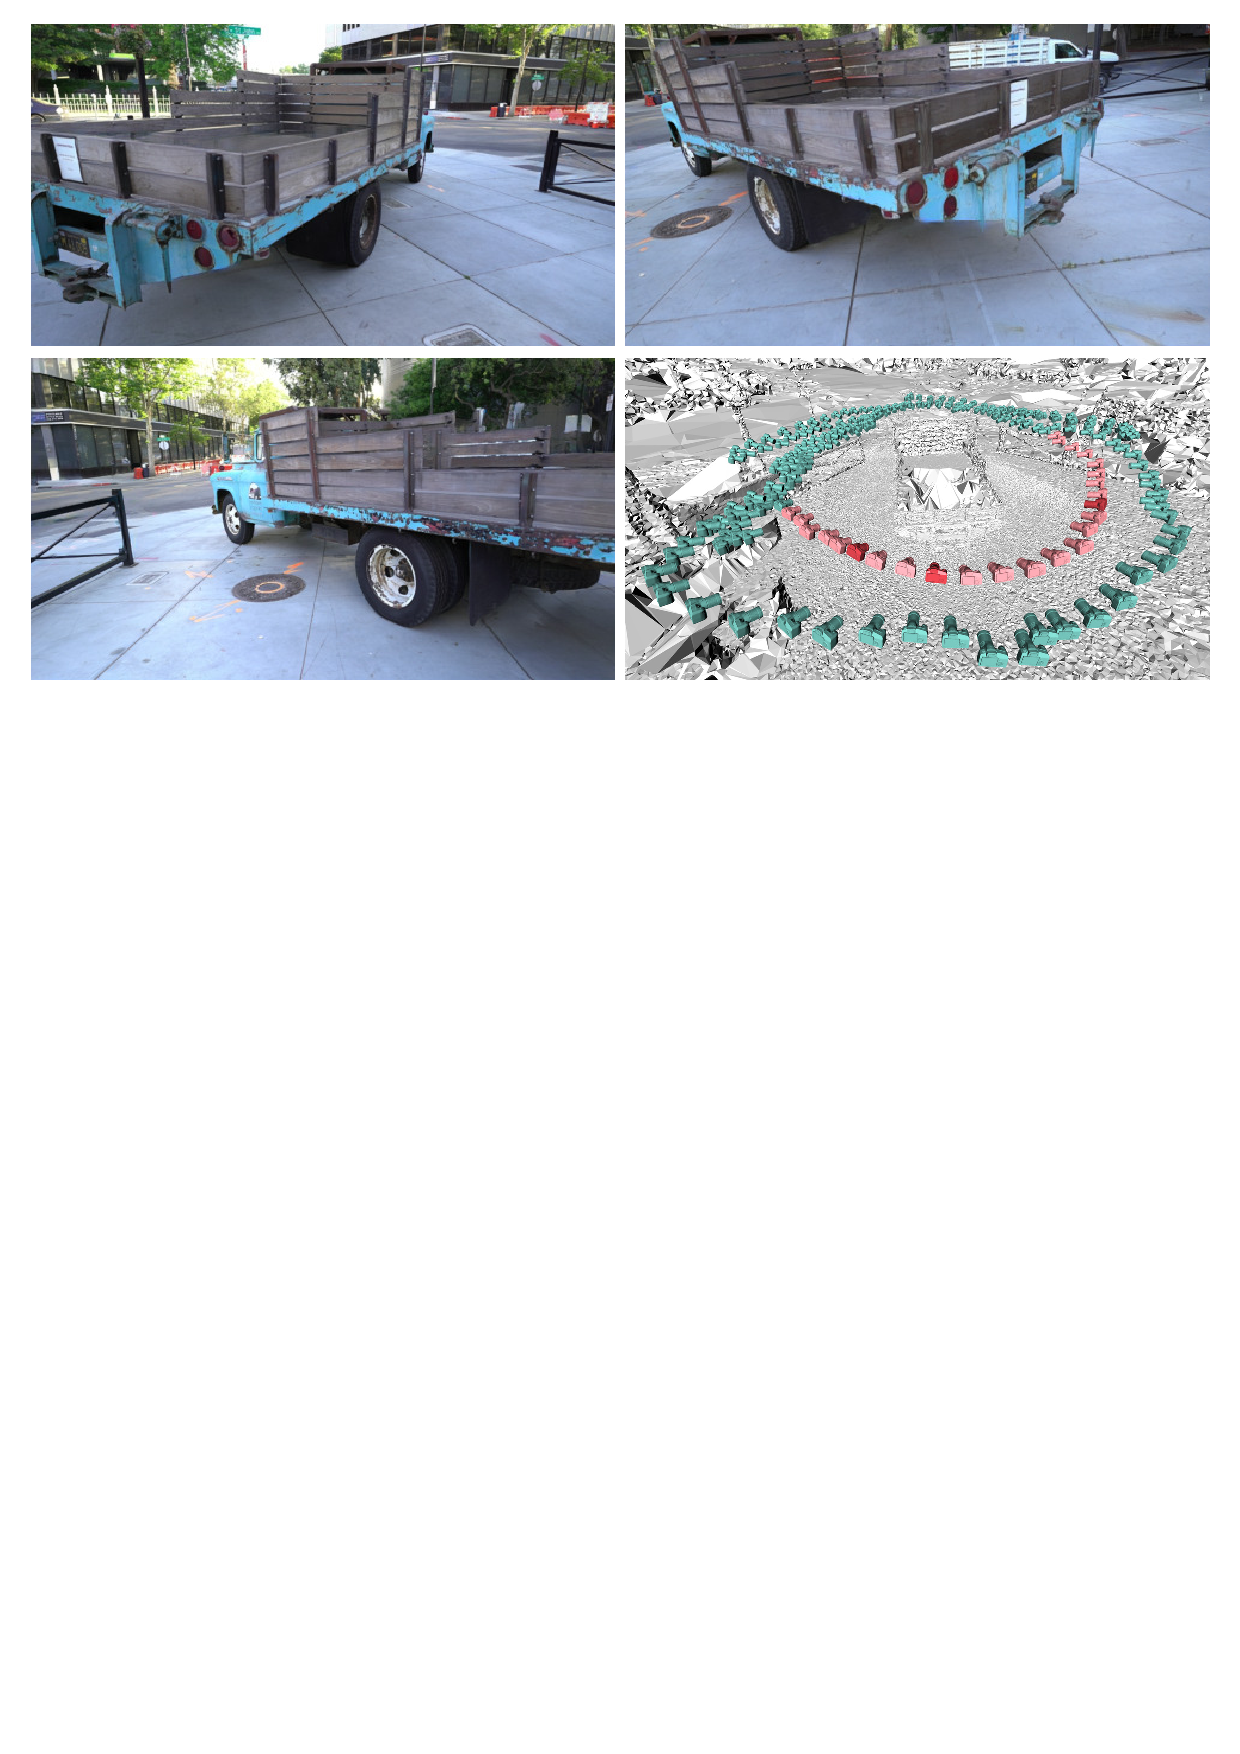
\includegraphics[width=0.95\textwidth]{figures/FreeViewSynthesis.pdf}
    \caption{新视图合成的示意图\cite{riegler2020free}。前三张图是合成的新视图,最后一张图阐明了绿色相机位姿下的图像作为输入,推理红色相机位姿的新视图。}
    \label{fig:FreeViewSynthesis}
\end{figure}
\newpage

根据前期调研,新视图合成技术有着广泛的应用前景,市场需求庞大,急需可快速合成高质量新视图的系统。而在实际应用中,限于应用需求和经济成本等因素的考量,市场上的大多产品仍存在着许多问题,比如无法在任意角度合成高质量图像,另外渲染新视图的时间过长,这些都严重影响了用户体验。而本身,三维场景具有一定复杂性,市面上的很多软件在渲染之前需要进行复杂的三维建模,这很考验硬件的算力和内存。这些都增加了系统的实现难度。

具体地,现有的系统中存在以下一些问题:1) 当前市场上的三维渲染的软件难以根据稀疏视图,在任意视角下渲染出高质量的新视图;
2) 目前的三维渲染系统大都需要根据深度信息进行三维建模,这需要使用 RGBD 相机,对硬件设备要求较高;
3) 目前市场上还没有直接可应用的面向快速新视图合成的交互系统;4) 现有的新视图合成模型需要在空间内进行大量采样,计算时间成本较高,难以完成 PC 端的快速交互需求。

如果想要把新视图合成技术很好地应用在虚拟现实等技术上,那么必须能够在任意视角下合成几乎与真实场景相同的图像。这在合成场景下是可能实现的,但是在真实场景中,无法获得准确的相机位姿、光照条件难以建模等问题都限制了更好的体验,新视图合成仍面临着许多挑战。

% 主要挑战是通过给定稀疏的观测图像来推断场景的三维几何结构,以及对场景中遮挡和看不见的地方进行修补。在经典计算机视觉中,基于图像的渲染 (Image-based Rendering, IBR\cite{debevec1998efficient,kee2013exposing}) 方法通常依赖于基于优化的多视图立体 (Multi-View Stereo, MVS) 方法,以将重构场景的几何形状并将观测转到新视图的坐标系中。然而,如果只有少量观测图像可用,场景包含依赖视图的影响或者新视角下大部分没有被观测的图像覆盖到,那么 IBR 可能失效会导致出现鬼影或者空洞等效果。最近,随着深度学习的发展,基于深度学习的神经渲染方法\cite{tewari2020state}被提出,旨在合成更高质量的新视图。2020年,Mildenhall等人\cite{mildenhall2020nerf}提出了基于神经辐射场 (Neural Radiance Fields, NeRF) 的方法去合成新视图,这使得神经渲染一度成为最优秀的新视图合成方法。NeRF 基于给定的稀疏图像,仅使用较为简单的全连接网络去隐式表达场景信息,最后使用体绘制的方法合成新视图。NeRF 是目前新视图合成任务中的渲染效果最佳的方法,但是由于使用体绘制进行渲染,要求必须在空间内进行大规模采样,这一方面会带来巨大的时间开销,另一方面采样点的位置的准确性将决定了神经辐射场拟合的准确性。



经典的基于图像的渲染 (Image-based Rendering, IBR\cite{kee2013exposing}) 方法可以完成以上任务,IBR 通常依赖于基于优化的多视图立体 (Multi-View Stereo, MVS) 方法,以此重构场景的几何结构。然而,如果只有少量观测图像可用,场景包含依赖视图的影响或者新视角下大部分没有被观测的图像覆盖到,那么 IBR 可能失效会导致出现鬼影或者空洞等效果。此外该方法需要对三维场景进行精细的三维重建,这会带来极大的计算开销,因此传统的基于图像的渲染方法难以应用到实际场景中。随着深度学习的发展,基于深度学习的神经渲染方法开始在新视图合成任务上展现出其惊人的渲染效果。
2020年,Mildenhall等人\cite{mildenhall2020nerf}提出了基于神经辐射场 (Neural Radiance Fields, NeRF) 的方法去合成新视图,这使得神经渲染一度成为最优秀的新视图合成方法。NeRF 基于给定的稀疏图像,仅使用较为简单的全连接网络去隐式表达场景信息,最后使用体绘制的方法合成新视图。如果有一个系统能够使用基于 NeRF 的方法快速渲染出高质量的新视图,那么将极大地提升用户体验。因此,在这样的需求下,本文致力于将具有最佳渲染效果的 NeRF 技术设计并实现成完整的新视图合成系统,并在不损失精度的情况下对其渲染过程进行加速。

NeRF 是目前新视图合成任务中的渲染效果最佳的方法,但是由于使用体绘制进行渲染,要求必须在空间内进行大规模采样,这一方面会带来巨大的时间开销,另一方面采样点的位置的准确性将决定了神经辐射场拟合的准确性。

本文主要关注的是渲染时间长这一问题。NeRF 为了获取对渲染图象贡献较高的采样点,同时优化两个神经网络,使用 coarse 网络的输出去估计采样点的分布情况,然后基于此分布进行二次采样并通过 fine 网络预测的颜色和体密度进行数值积分计算出 2D 图像对应像素的 RGB 值,这带来了极大的时间开销。同时为了拟合更准确的神经辐射场,NeRF 使用了较深的神经网络,这也增加了推理新视图过程的时间成本。以上正是本文需要加速的地方。

在这样的背景下,本文研究了基于神经辐射场的新视图合成的相关技术,认为基于深度学习的神经渲染方法存在着提升空间,并对现有方法 NeRF 进行了优化,设计并训练了可以快速合成高质量新视图的神经渲染模型。渲染效果受数据集的影响,一般来说合成场景下质量会相对好些,因为真实场景下问题比较多,比如相机标定不严格、相机位姿估计不准,照片畸变严重,光照条件难以建模等等。

最终,本文结合 NeRF 的技术以及查询表缓存加速的相关技术实现了快速合成新视图的神经辐射场渲染具体方法,并设计和实现了一个快速新视图合成的系统,完成了 PC 客户端的相关应用。与现有产品相比,该系统可以基于给定的稀疏图像,快速渲染出任意新视角下的图像,提供几乎和 NeRF 质量相同的新视图。

本课题来自于PixTalks公司的实际应用需求。

\section{国内外研究现状}
% \subsection{新视图合成相关系统应用现状}
% 为了了解新视图合成相关系统的现状,本文对相关产品进行了调研。目前市面上暂无直接具有新视图合成功能的系统或软件,都是将新视图合成技术嵌入到系统或软件的内部。    

\subsection{基于图像的神经渲染方法研究现状}
在计算机图形和计算机视觉中,基于图像的渲染方法通常是依靠场景的一组二维图像来生成三维模型,然后渲染该场景的一些新视图。一般基于图像的渲染 (Image-based Rendering, IBR) 方法根据是否使用几何信息分成两类。几何信息用于将图像内容从捕获的图像重新投影到新的目标图像域。在目标图像域中,源图像的投影被混合以合成最终图像。这种简化的过程仅能为具有精确几何结构且具有捕获足够多视图的物体提供较为准确的结果。但是,由于依赖于视图的影响,以及不完善的几何信息或太少的源图像,可能会出现诸如重影,模糊,孔洞或接缝之类的伪影。

\begin{figure}[tbhp]
    \centering
    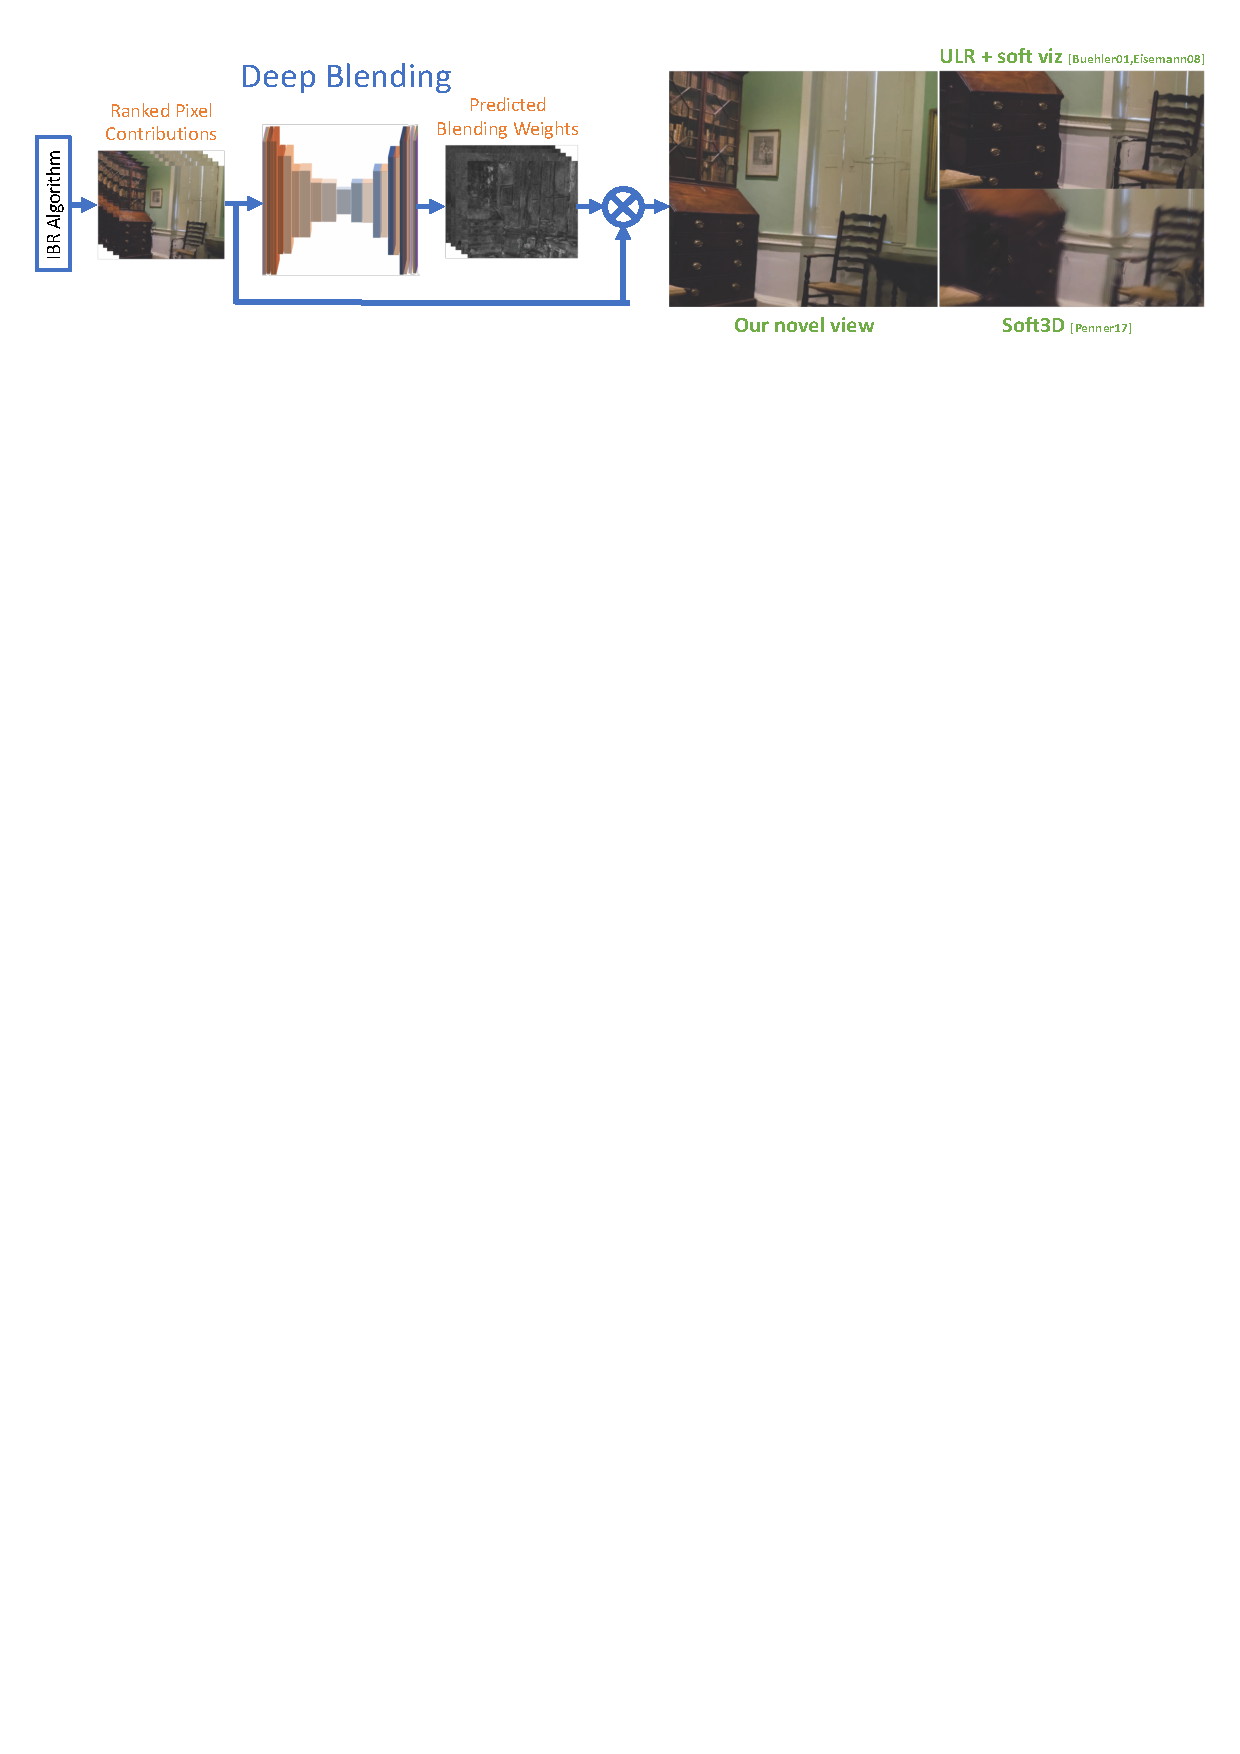
\includegraphics[width=0.95\textwidth]{figures/deepblending.pdf}
    \caption{DeepBlending\cite{hedman2018deep} 的框架结构,渲染效果较其他方法减少了伪影。}
    \label{fig:deepblending}
\end{figure}

为了解决上述问题,将经典的基于图像渲染的方法与现如今最火的深度学习网络的结合成基于 IBR 的神经渲染方法,这极大地提升了 IBR 的渲染效果。DeepBlending\cite{hedman2018deep}提出了一种广义网络来预测投影源图像的混合权重,以便在目标图像空间进行合成。DeepBlending 在室内场景中显示了惊人的效果,比经典的 IBR 方法具有更少的混合伪影,具体见图~\ref{fig:deepblending}。事实上,DeepBlending 是将 COLMAP\cite{schonberger2016structure} 和商用软件 Reality Capture 进行了结合,以此获取更为精细的几何结构信息。COLMAP 基于块匹配的多视图几何算法进行稠密重建,这能够非常好地重建场景中的细节,但是与此同时在纹理信息缺失的地方也会出现空洞。Reality Capture 的结果相对完整,但是对于场景级别的区域重建的较差。因此,上述两种方法是互补的,将它们进行结合可以获得非较为准确的几何模型信息,DeepBlending 就是使用上述几何信息,借助神经网络来学习如何将不一致的观测图像信息进行混合,最终确实获得了非常惊艳的效果。但是,该方法过于依赖 COLMAP 三维重建出的几何信息,当几何信息较少时渲染质量会严重下降并伴随伪影。此外,精细的三维重建会带来非常大的计算开销,这在实际中难以使用。因此这种经典的基于 IBR 的方法无法满足本系统的速度和质量需求。

%其他方法如 NPBG\cite{aliev2019neural} 和 NPCR\cite{dai2020neural} 使用比 mesh 更容易获得的点云作为三维代理几何体。由于点云自身的稀疏性特征,很可能会出现不应该观测到的点出现在新视角下,这是著名的 bleeding 现象。为了解决 bleeding 现象问题,NPBG 使用多分辨率的方式,将不同分辨率的特征图输入到后端网络中。不过,多分辨率的策略虽然解决了 bleeding 的问题,但是得到了相对模糊的渲染结果。	

\subsection{基于 NeRF 的新视图合成研究现状}
类似 DeepSDF\cite{park2019deepsdf},NeRF\cite{mildenhall2020nerf}借助深度学习的隐式表达方法,将三维几何场景中的光照和几何信息隐式表达在神经网络参数中,最后利用立体渲染的方法进行渲染。NeRF 算是基于图像的神经渲染方法中最具代表的工作了。NeRF 本身不需要任何的显式的几何信息,仅使用真实场景的 RGB 图像作为监督信号,使用深度神经网络自动推理相关几何以及光照信息。NeRF 凭借着其网络简单,渲染效果惊艳的特性,备受学术界和工业界的关注。自从 NeRF 的出现,基于神经辐射场的新视图合成相关工作开始大量涌现。

NeRF++\cite{zhang2020nerf++} 首次指出 NeRF 具有形状光线的歧义性问题,即 NeRF 在一个场景下训练好的网络,其对应的空间表示可能是错的,但是仍能在训练集上渲染出正确的结果。

%\begin{figure}[tbhp]
%    \centering
%    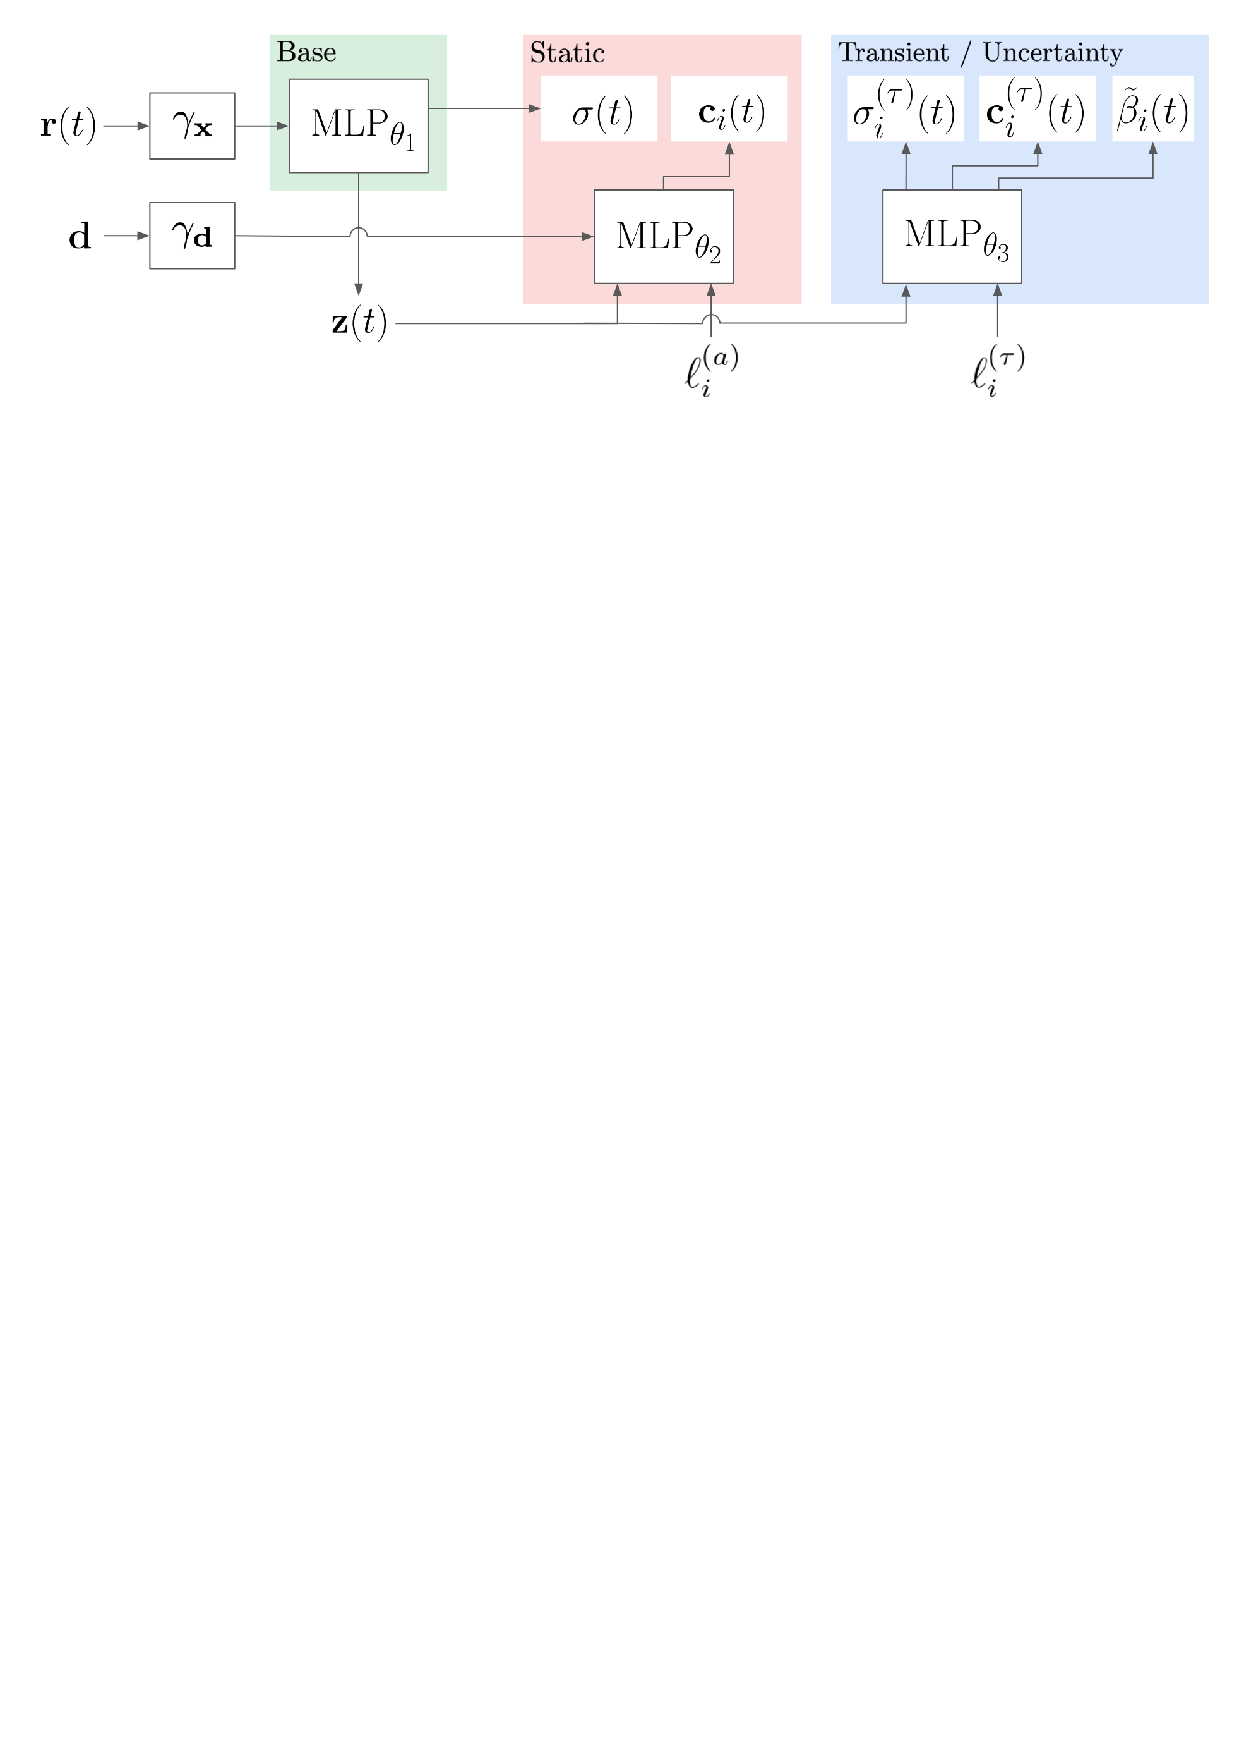
\includegraphics[width=0.95\textwidth]{figures/NeRF-W.pdf}
%    \caption{NeRF-W\cite{martin2020nerf}的网络框架示意图}
%    \label{fig:nerf-w}
%\end{figure}
%
%之后 NeRF-W\cite{martin2020nerf} (NeRF in the Wild) 对 NeRF 进行了另一种补充改进。由于 NeRF 假设输入的图像是由静态场景生成的图像,每张图所表示的场景具有相同的光照条件和几何结构,这在实际中是很难保证的。对于这个问题,如图~\ref{fig:nerf-w}所示,NeRF-W 给每张图片都预先编码了两个固定向量,分别是 $l_i^{\left(a\right)}, l_i^{\left(\tau\right)}$。其中,$l_i^{\left(a\right)}$ 是用来学习当前的光照条件,而 $l_i^{\left(\tau\right)}$ 是用来学习当前图像是否有动态物体遮挡,将这两个embedding 输入网络会输出一个不确定度。以上的做法让 NeRF-W 在真实场景下能够表现地更加鲁棒,在光照条件变化以及动态的场景下都取得了非常好的效果。

Yen-Chen等人\cite{yen2020inerf}基于位姿估计方法给 NeRF 提供了新的改进思路,推出了新工作 iNeRF。NeRF 在处理真是数据集的时候,位姿是通过COLMAP\cite{schonberger2016structure}进行计算的,然而这并不能获得绝对精准的位姿,也即送入网络的采样点是不准确的,那么也无法准确拟合真是场景的神经辐射场。如图~\ref{fig:inerf} 所示的是 iNeRF 的网络框架,注意到,颜色的均方误差对坐标是可微的,而坐标对相机位姿也是可微的,因此,可以在训练神经辐射场的同时对位姿进行优化,具体是采用神经网络的反向传播算法进行优化的。此外,为了更有效地优化位姿,iNeRF 使用了 ROI 采样方式,即对感兴趣的区域进行采样优化,这样能显著缓解直接采样一张图片带来的内存开销大的问题。iNeRF 通过位姿矫正,最终在真实场景下显著提升了 NeRF 的渲染质量。不过,由于训练时每一张图都要单独优化位姿,而渲染时相机位姿仍然是不准确的,因此本系统暂不考虑位姿的问题。

\begin{figure}[tbhp]
    \centering
    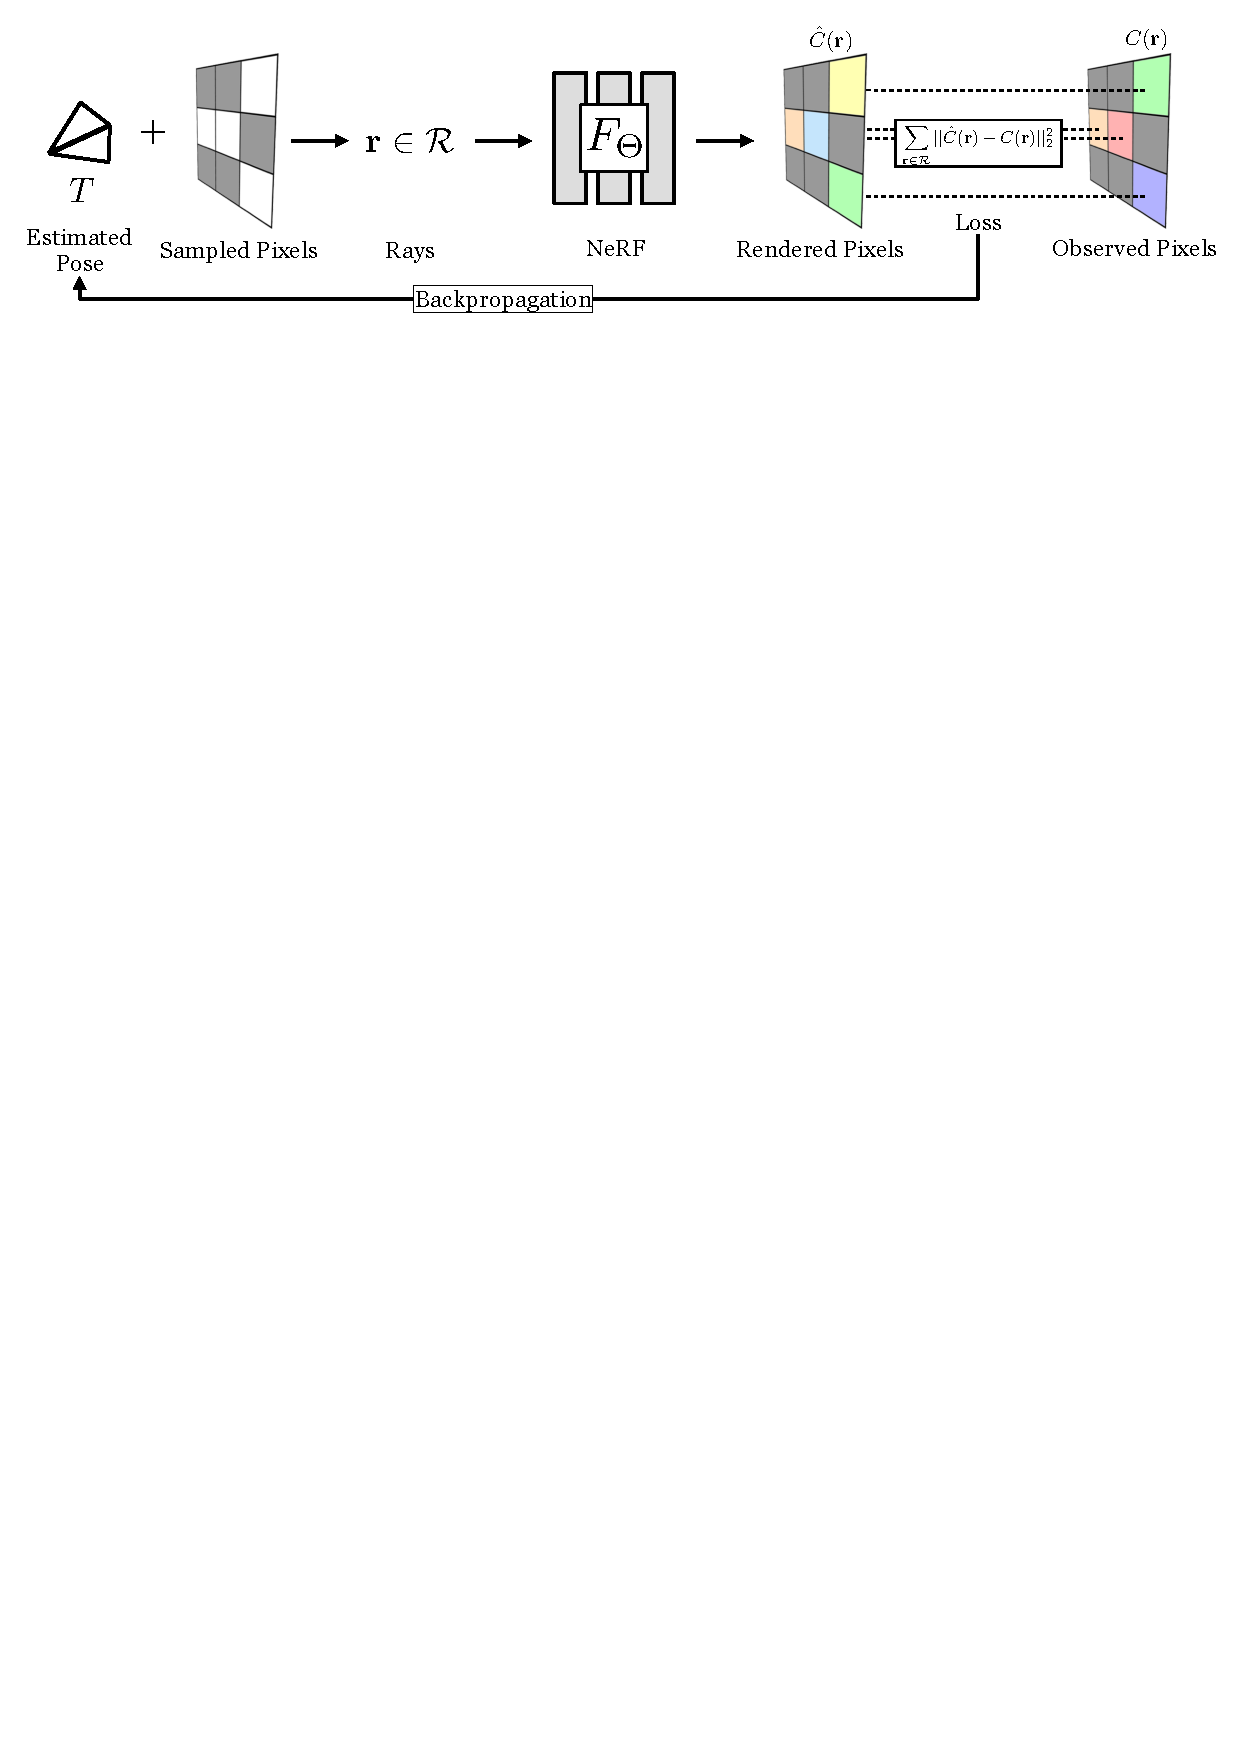
\includegraphics[width=0.95\textwidth]{figures/iNeRF.pdf}
    \caption{iNeRF\cite{yen2020inerf}的网络框架示意图}
    \label{fig:inerf}
\end{figure}

上述方法都还是基于多层感知机 (MLP, Multilayer Perceptron) 训练的。下面介绍一些对 NeRF 网络上进行的一些改进的工作。PixelNeRF\cite{yu2020pixelnerf} 使用卷积神经网络 (Convolutional Neural Networks, CNN) 提取的特征,仅需要少量图片作为输入就可以合成新视角下的图像,并有一定的泛化能力。GRF\cite{trevithick2020grf}使用 CNN 提取包含光线属性的特征,并使用 attention 机制将采样点在不同视角下的特征进行聚合,极大地提升了渲染质量。GRAF\cite{schwarz2020graf} 使用对抗生成网络 (Generative Adversarial Networks, GAN) 对 NeRF 进行改进,使之具有较强的泛化能力。但是,以上这些基于网络的改进方法都使得网络变得过于复杂,有些违背 NeRF 网络简洁的初衷,会使得训练和渲染的时间过长,这不能满足用户对于快速合成新视图的需求,几乎无法应用到实际的系统中。

\begin{figure}[htb]
	\centering
	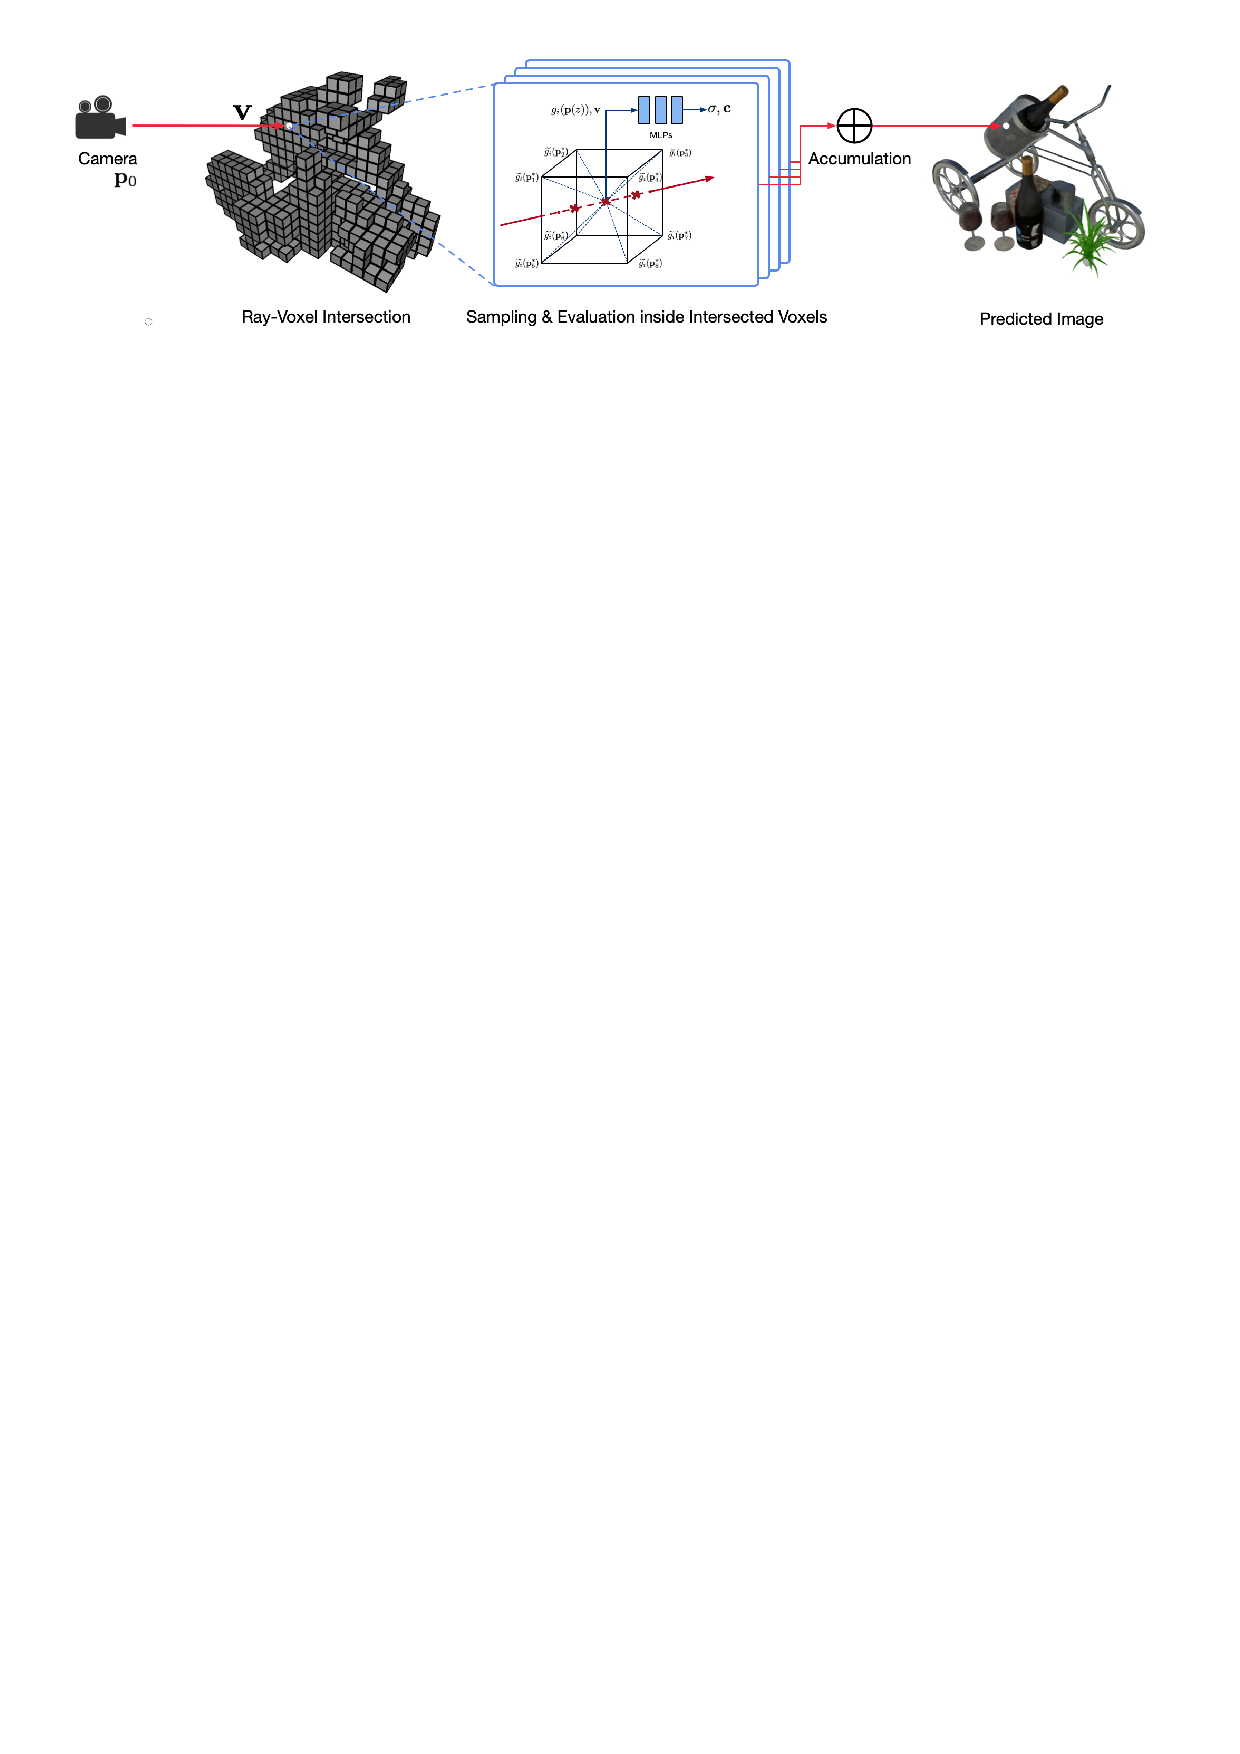
\includegraphics[width=0.95\textwidth]{figures/NSVF.pdf}
	\caption{NSVF\cite{liu2020neural}的网络框架示意图}
	\label{fig:nsvf}
\end{figure}

下面介绍一些基于 NeRF 的加速方法。由于 NeRF 需要在相机光线上进行大量的采样,这些采样点都要经过网络,而 NeRF 自身又使用了两个网络进行训练,因此 NeRF 的渲染是很慢的。如图~\ref{fig:nsvf},为了给 NeRF 加速,NSVF\cite{liu2020neural} 首先提出将空间划分为若干体素,使用自我裁剪的方法去掉体密度较小的体素,渲染的时候只需找到相机光线第一个穿过的体素,根据该体素八个顶点对应的特征进行插值编码并送入下游 MLP 预测出颜色和体密度,这避免了大量的采样计算,显著加速了新视图合成的过程。但是,NSVF 仅适用于简单的三维物体,在复杂的真实场景下渲染新视图的质量较差,甚至会出现鬼影,因此并不适合在本系统上使用。Lindell等人\cite{lindell2020autoint}提出了一种利用自动积分来进行渲染加速的方法 AutoInt。AutoInt 是通过隐式网络学习到闭式解求积分,从而取代了 NeRF 的数值积分,最终能为 NeRF 渲染过程加速10倍。不过,就 PSNR 来看,AutoInt 在合成数据集 Synthetic-NeRF 上平均比 NeRF 低\SI{5.4}{dB},这是一种重视加速但牺牲了很多质量的方法,并没有真正做到在不失精度的情况下对渲染进行加速。上述介绍的加速方法未能保证不损失精度情况下对 NeRF 进行加速,不符合本系统的需求,因此本文最终依旧使用最经典应用场景最丰富的 NeRF 技术并对其进行无精度损失的加速,最终完成整个快速新视图合成系统的构建。

\section{本文的主要工作与贡献}
% 基于神经辐射场的快速新视图合成系统的设计与实现中存在以下一些问题:1) 当前市场上的三维渲染的软件难以根据稀疏视图,在任意视角下渲染出高质量的新视图;
% 2) 目前的三维渲染系统大都需要根据深度信息进行三维建模,这需要使用 RGBD 相机,对硬件设备要求较高;
% 3) 目前市场上还没有直接可应用的面向快速新视图合成的交互系统;4) 现有的新视图合成模型需要在空间内进行大量采样,计算时间成本较高,难以完成 PC 端的交互需求。

本文将 NeRF 技术和查询表技术进行有机融合,设计并实现了基于神经辐射场的快速新视图合成系统。本文根据 NeRF 的特性提出了基于神经辐射场进行加速合成新视图的框架, 将其命名为 F-NeRF,通过 NeRF 预测的体密度有效地提取到物体的几何结构并缓存到查询表中,这一方面辅助了获取物体表面附近的对计算颜色有高贡献的采样点,另一方面减少了一个网络的开销,同时也简化了网络,这显著加速了渲染的过程。最后,本文将这 F-NeRF 这一方法有效地部署到 PC 端,将其实现成可交互的系统。

具体地,本文的主要工作与贡献如下:
\begin{enumerate}
    \item [1)] 本文基于 NeRF 预训练的网络预测的体密度信息构建出一个可以表征在物体内外的查询表结构,这一方面直接减少了查询表的尺寸,另一方面该查询表可以直接为空间内任意一点提供 NeRF 网络中间层的特征,这加快了神经网络的正向传播速度。
    \item [2)] 在缓存了上述查询表的基础上,本文改进了 NeRF 的采样过程,通过查询表找到光线上离物体表面最近的内点,使得 NeRF 可以仅在此点附近进行采样,从而不必再使用两个网络,这显著加速了 NeRF,同时这正是本文的核心贡献。
    \item [3)] 为了补偿查询表分辨率不够带来的精度损失,本文对 F-NeRF 进行再训练,将渲染质量提升到原 NeRF 的水平。
    \item [4)] 本文在公开的数据集上做了大量对比验证实验。在公开合成数据集 Synthetic-NeRF 和真实场景数据集 LLFF-NeRF 上,与 NeRF 相比,我们提出的 F-NeRF 方法分别加速 3.2 倍和 3.4倍。 
    \item [5)] 本文设计并实现了基于 NeRF 的快速新视图合成的系统,完成了相应的 PC 端的应用,并对该系统进行了详细的需求分析以及架构设计,最后将本文的方法实现并部署到了 PC 端,经过详细地测试,该系统满足实际应用需求。
\end{enumerate}

%1) 使用预训练的 NeRF 网络,构建出一个可以表征在物体内外的查询表,该查询表可以直接为空间内任意一点提供 NeRF 网络中间层的特征,这加快了神经网络的正向传播速度。
%2) 在缓存了上述查询表的基础上,本文改进了 NeRF 的采样过程,通过查询表找到光线上离物体表面最近的内点,使得 NeRF 可以仅在此点附近进行采样,从而不必再使用两个网络,这显著加速了 NeRF,同时这正是本文的核心贡献。3) 本文设计并实现了基于 NeRF 的快速新视图合成的系统,完成了相应的 PC 端的应用,并对该系统进行了详细的需求分析以及架构设计,最后将本文的方法实现并部署到了 PC 端,经过详细地测试,本文方法在合成场景和真实场景下的渲染速度对 NeRF 分别加速3.2倍和3.4倍,该系统满足实际应用需求。


\section{本文的章节安排}

第一章是绪论,主要阐述了本文研究工作的背景与意义,指出了本文研究问题的难点,并介绍了本文的主要研究工作和贡献,对国内外相关工作的研究现状的充分调研与分析,最后对本文的组织架构进行安排。

第二章是相关理论和技术,主要介绍了基于神经辐射场的快速新视图合成系统应用的核心技术和算法。

第三章是本文的主要工作,主要介绍了本文方法的问题定义,本文方法的预备工作,然后详述了我们改进的基于神经辐射场的新视图合成加速方法。

第四章是本文的实验部分。主要阐述了实验的基本设置,包含开发环境、数据集等等,其次介绍了实验实现的具体细节以及相关评测指标。最后通过大量对比实验来验证本文提出的方法的有效性,同时对一些实验结果进行分析和讨论。

第五章是系统设计与实现,主要介绍了将本文提出的 F-NeRF 方法应用到系统上的具体实现与架构设计。详细阐述了本系统的需求分析,包含主要用例分析,以及具体的系统架构设计,最后介绍了将本系统的模型移植到 C++ 代码上的方法。

第六章是系统的部署与展示,主要介绍了本文系统的开发与运行环境,对经典的测试用例进行了详尽的步骤说明,根据用例步骤完成了功能测试。从测试结果看,系统各项功能均能正常运行,合成新视图速度快且质量高。

第七章为总结和展望部分。总结了本文的主要工作和贡献,并指出工作中的不足之处。提出在未来研究过程中的可能的研究方向,并对可继续完善的方面进行展望。
% \begin{enumerate}
%     \item 主体部分包括引言 (前言),国内外文献综述,正文, 结语,参考文献。要求图表清晰,叙述流畅,章节有序,层次 分明。\\
%     引言 (前言)部分内容主要为本研究课题的学术背景及理论与实际意义;本研究课题的来源及主要研究内容;建立研究的线索与思路。

%     \item 文中的图、表、公式等,一律用阿拉伯数字按章顺序编号。如图 1-1、图2-2, 表 1-1、表 2-1,公式 (1-1) 等。图序及图名置于图的下方,居中排列;表序及表名置于表的上方,居中排列。详见第\ref{figures_tables}章的说明。

%     \item 参考文献
%     \begin{enumerate}
%         \item 参考文献为论文中所有引文、引用观点以及对论文有重要影响和启发的文献;
%         \item 参考文献按在论文中出现的先后依次排序;个别学科若通用该学科惯用的排序规范,可以例外;
%         \item 参考文献内容一般排列在论文末尾 (论文篇幅较大且引用文献较多的,可在每章末尾注出),序码与论文加注处对应;
%         \item 参考文献标注格式: 使用国标GB/T 7714-2015标准, 建议使用工具自动控制引文格式, 
%         以保证格式规范。
%         该\LaTeX{}模板已经对引文格式做了配置,
%         用户需要将所需参考文献的信息存在 \texttt{bib} 格式的文件\texttt{ref/refs.bib}中, 
%         通过 \verb|\cite{}|命令在恰当位置引用 (详见第\ref{citations}章的说明)。
%         \texttt{bib}文件可从文献管理工具导出或自己用 \texttt{JabRef} 等软件编辑。
%     \end{enumerate}

%     \item 注释:可以用 “脚注”或 “文后注”来标注引用著作中的一些观点和案例,但全文标注方式应统一。
% \end{enumerate}


\cleardoublepage
% !TeX root = ../main.tex

\chapter{相关技术和理论概述}\label{equations}
本文主要研究的内容是神经辐射场在新视图合成上的加速,因此本章首先主要介绍神经三维形状表示法,新视图合成和基于图像的渲染方法。随着深度学习的发展,当今效果最佳的新视图合成算法都是基于深度学习的,因此接下来会概述深度学习的原理和发展状况,并重要介绍基于深度学习的神经辐射场的立体渲染方法。最后介绍一下查询表的概念,以及查询表在逐点网络上的加速应用,为本文方法的展开做好铺垫。

\section{神经三维形状表示法}
三维物体的形状表示有多种方法,传统的基于数据驱动的三维学习表示方法可以总体上分为三类:基于点,基于网格,基于体素的方法。此外,还有最新的基于深度学习的三维形状表示方法,下面对以上四种表示方法分别进行阐述。

\subsection{基于点的表示方法} 
基于点的方法一般指的是点云(如~\ref{fig:stanfordRabbit}所示的第一个)这种表示,点云是指空间中一组点的集合,每一个点都包含 X,Y,Z 三个坐标。它是一种轻量级的三维表示方式,与匹配许多传感器(例如雷达,深度相机)提供的原始数据非常匹配,因此非常适合应用在三维学习技术上。例如 PointNet\cite{qi2017pointnet,qi2017pointnet++} 这篇非常经典的点云工作,使用最大池化操作来提取全局特征,之后这项技术被广泛用作点生成网络\cite{yang2017foldingnet,achlioptas2018learning}的编码器。此后点云学习方面又涌入了大量的 PointNet 风格的相关工作。然而,点云这种表示方法有着很明确的限制,它们不适用于描述拓扑结构,同时也不适合用以生成紧致的表面。

\subsection{基于网格的表示方法}
许多方法使用预定义模板的网格,它们表征了一系列相似形状的物体,例如可变形的人体部位,其中一些模型\cite{2017Deformable}展示了高保真的形状生成结果。其他的最近工作\cite{baque2018geodesic}使用多边形立方体映射\cite{tarini2004polycube}对形状进行优化。虽然模板网格的使用很方便,并且自然地提供了三维对应,但它只能对具有固定网格拓扑的形状进行建模。其他基于网格的方法使用已有的\cite{sinha2016deep,maron2017convolutional}或者学习的\cite{groueix2018papier,ben2018multi}参数化技术通过二维平面来描述三维曲面。这种表示的质量取决于参数化算法,这些算法通常对输入网格质量和切割策略非常敏感。为了解决这个问题,最近的数据驱动方法\cite{yang2017foldingnet}学习深度网络的参数化任务。然而,他们报告说需要多个平面来描述复杂的拓扑,但是生成的曲面片没有缝合,即生成的形状没有闭合。为了生成闭合网格,可以使用球体参数化\cite{groueix2018papier,ben2018multi},但生成的形状仅限于拓扑球体。其他与网格学习相关的工作建议对网格\cite{defferrard2016convolutional,verma2018feastnet}或一般图\cite{bruna2013spectral}使用新的卷积和池化运算。网格表示三维物体的直观感受如~\ref{fig:stanfordRabbit}所示。

\subsection{基于体素的表示方法}
在三维计算机图形学上,体素代表了三维空间中规则格点所对应的值。与二维位图中的像素一样,体素本身通常不使用其值显式编码其位置(即坐标)。取而代之的是,渲染系统根据其相对于其他体素的位置(即其在构成单个体积图像的数据结构中的位置)来推断体素的位置。体素算是像素由二维空间直接推广到三维空间,有着不少共性。基于体素的学习方法中最直接的变体就是占据栅格。但是由于计算和内存开销呈三次方的增长趋势,因此当前的方法只能处理较低分辨率的情况。因此,基于体素的方法\cite{20153D,Choy20163D}无法保留精细的形状细节,由如~\ref{fig:stanfordRabbit}所示的第三个图就能明确这一点,此外,体素在视觉上显示与高保真度形状有显著差异,因为渲染时法线不平滑。基于八叉树\cite{Tatarchenko2017Octree,riegler2017octnet,hane2017hierarchical}的方法一定程度上减轻了稠密体素方法的计算和内存限制,但是提升后的分辨率依然没有产生很好的视觉响应。

\begin{figure}[t]
  \centering
  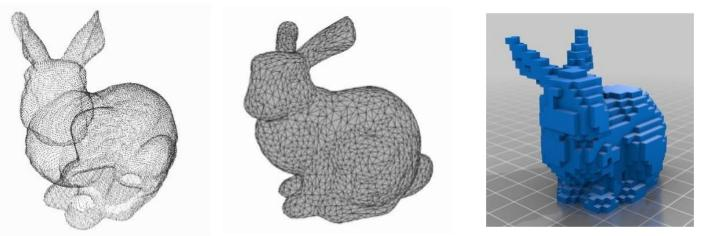
\includegraphics[width=0.9\linewidth]{stanfordRabbit.jpg}
  \caption{三种传统的三维表示方式(点云,网格,体素)}
  \label{fig:stanfordRabbit}
\end{figure}

\subsection{基于深度学习的表示方法}
计算机视觉中最近一个有前景的方向是用多层感知机 MLP 的权值编码对象和场景,MLP 直接从三维空间位置映射到形状的隐式表示,例如该位置的有符号距离\cite{curless1996volumetric},如图~\ref{fig:sdf}所示是有符号距离函数 (Signed Distance Fuction, SDF)在三维表示上的应用。然而,这些方法到目前为止还无法再现具有复杂几何体的真实场景,其保真度与使用离散表示(如三角形网格或体素网格)表示场景的技术相同。

最近的工作通过优化将 xyz 坐标映射到 SDF 函数\cite{jiang2020local,park2019deepsdf,chabra2020deep}或占据域\cite{genova2020local,mescheder2019occupancy}的深度网络,研究了连续三维形状作为水平集的这种隐式表示。然而,这些模型受到三维几何体 ground truth 的需求的限制,这些几何体通常是从合成的三维形状数据集(例如如 ShapeNet\cite{chang2015shapenet} )获得的。随后的工作通过构造可微的渲染函数,使得神经隐式形状表示仅使用 2D 图像进行优化,从而放宽了对三维形状 ground truth 的要求。Niemeyer 等人\cite{niemeyer2020differentiable}将曲面表示为 3D 占据场,并使用数值方法找到每条光线的曲面交点,然后使用隐式微分计算精确导数。每个光线相交位置都作为神经 3D 纹理场的输入,该纹理场预测该点的颜色。Sitzmann 等人\cite{sitzmann2019scene}使用了一种不太直接的神经 3D 表示法,只需在每个连续的 3D 坐标上输出一个特征向量和 RGB 颜色,并提出了一种可微绘制函数,该函数由一个沿每条射线行进的递归神经网络组成,以确定曲面的位置。

\begin{figure}[t]
  \centering
  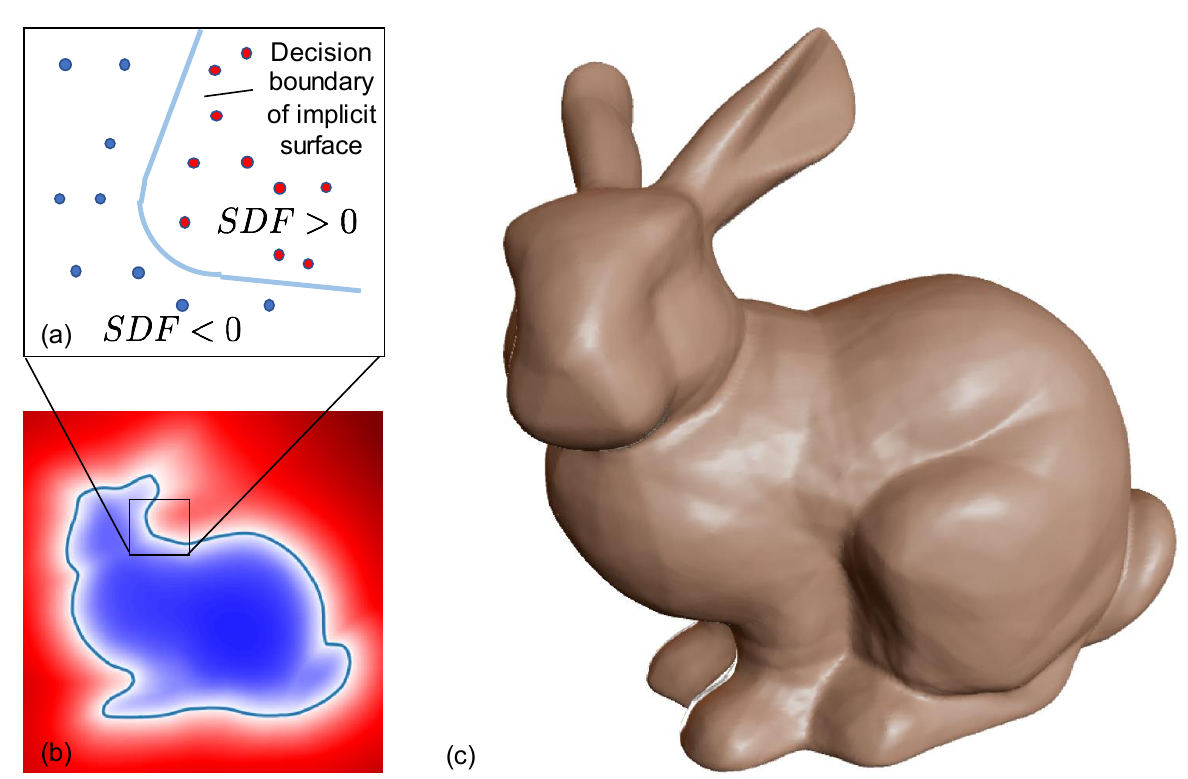
\includegraphics[width=0.8\linewidth]{sdf.png}
  \caption{SDF 函数表示法应用于斯坦福兔子,图片来自于 DeepSDF\cite{park2019deepsdf}}
  \label{fig:sdf}
\end{figure}

\section{新视图合成和基于图像的渲染}
新视图合成在计算机视觉与计算机图形学这样的交叉领域上是一个长期的问题。所谓新视图合成指的是给定一系列(或者单张)已知相机位姿的视图,由这些视图合成出未知位姿的视图。新视图合成的过程如图~\ref{fig:novelviewsynthesis}所示。对于给定稀疏视角采样的新视角合成问题,计算机视觉和图形学社区在从观测到的图像中预测传统几何表示的问题上取得了很多进展。一类流行的方法是使用具有要么漫反射\cite{Waechter2014Let}的,要么依赖视角\cite{debevec1996modeling, wood2000surface}的外观的那些 mesh-based(基于网格) 的场景表示。可微分的光栅化器\cite{loper2014opendr,chen2019learning,genova2018unsupervised,liu2019soft}或路径跟踪器\cite{li2018differentiable,nimier2019mitsuba}可以直接通过使用梯度下降法来优化再现一组输入图像的网格表示。然而,基于图像重投影的网格梯度下降的优化是十分困难的,可能是由于局部极小值或 loss 的调整不佳所致。此外,这种策略\cite{li2018differentiable}要求在优化之前提供具有固定拓扑的模板网格作为初始化,这通常对于不受约束的真实场景是不可用的。

另一类方法使用体积表示法来解决从一组输入 RGB 图像中进行高质量逼真的视图合成的任务。体积表示法是能够真实地表达复杂的形状和物体,非常适合基于梯度的优化,比基于网格的方法产生的视觉干扰更少。早期的体积方法\cite{kutulakos2000theory,szeliski1998stereo}使用观察到的图像直接为体素网格着色。最近,几种方法\cite{flynn2019deepview,mildenhall2019local,srinivasan2019pushing,zhou2018stereo}使用了多个场景的大型数据集来训练深层网络,这些深层网络从一组输入图像中预测采样的体积表示,然后使用其中一种 alpha 合成\cite{porter1984compositing}或沿光线学习的合成,以在测试时渲染新视图。其他工作需要针对每个特定场景优化了卷积神经网络和采样体素网格的组合网络,这样 CNN 可以补偿来自低分辨率体素网格\cite{sitzmann2019deepvoxels}的离散化伪像或允许预测的体素网格根据输入时间或动画控制而变化。尽管这些体积化的技术在新视图合成中取得了令人印象深刻的效果,但是由于它们是离散采样的,它们在时间和空间上的复杂性从根本上限制了它们缩放到高分辨率图像的能力,渲染高分辨率的图像需要 3D 空间的更精细的采样。NeRF 通过在全连接的深度神经网络的参数范围内编码连续的体积来规避此问题,这不仅比以前的体积方法产生了更高质量的渲染,而且只需要这些采样体积表示的存储成本的一小部分。

\begin{figure}[t]
  \centering
  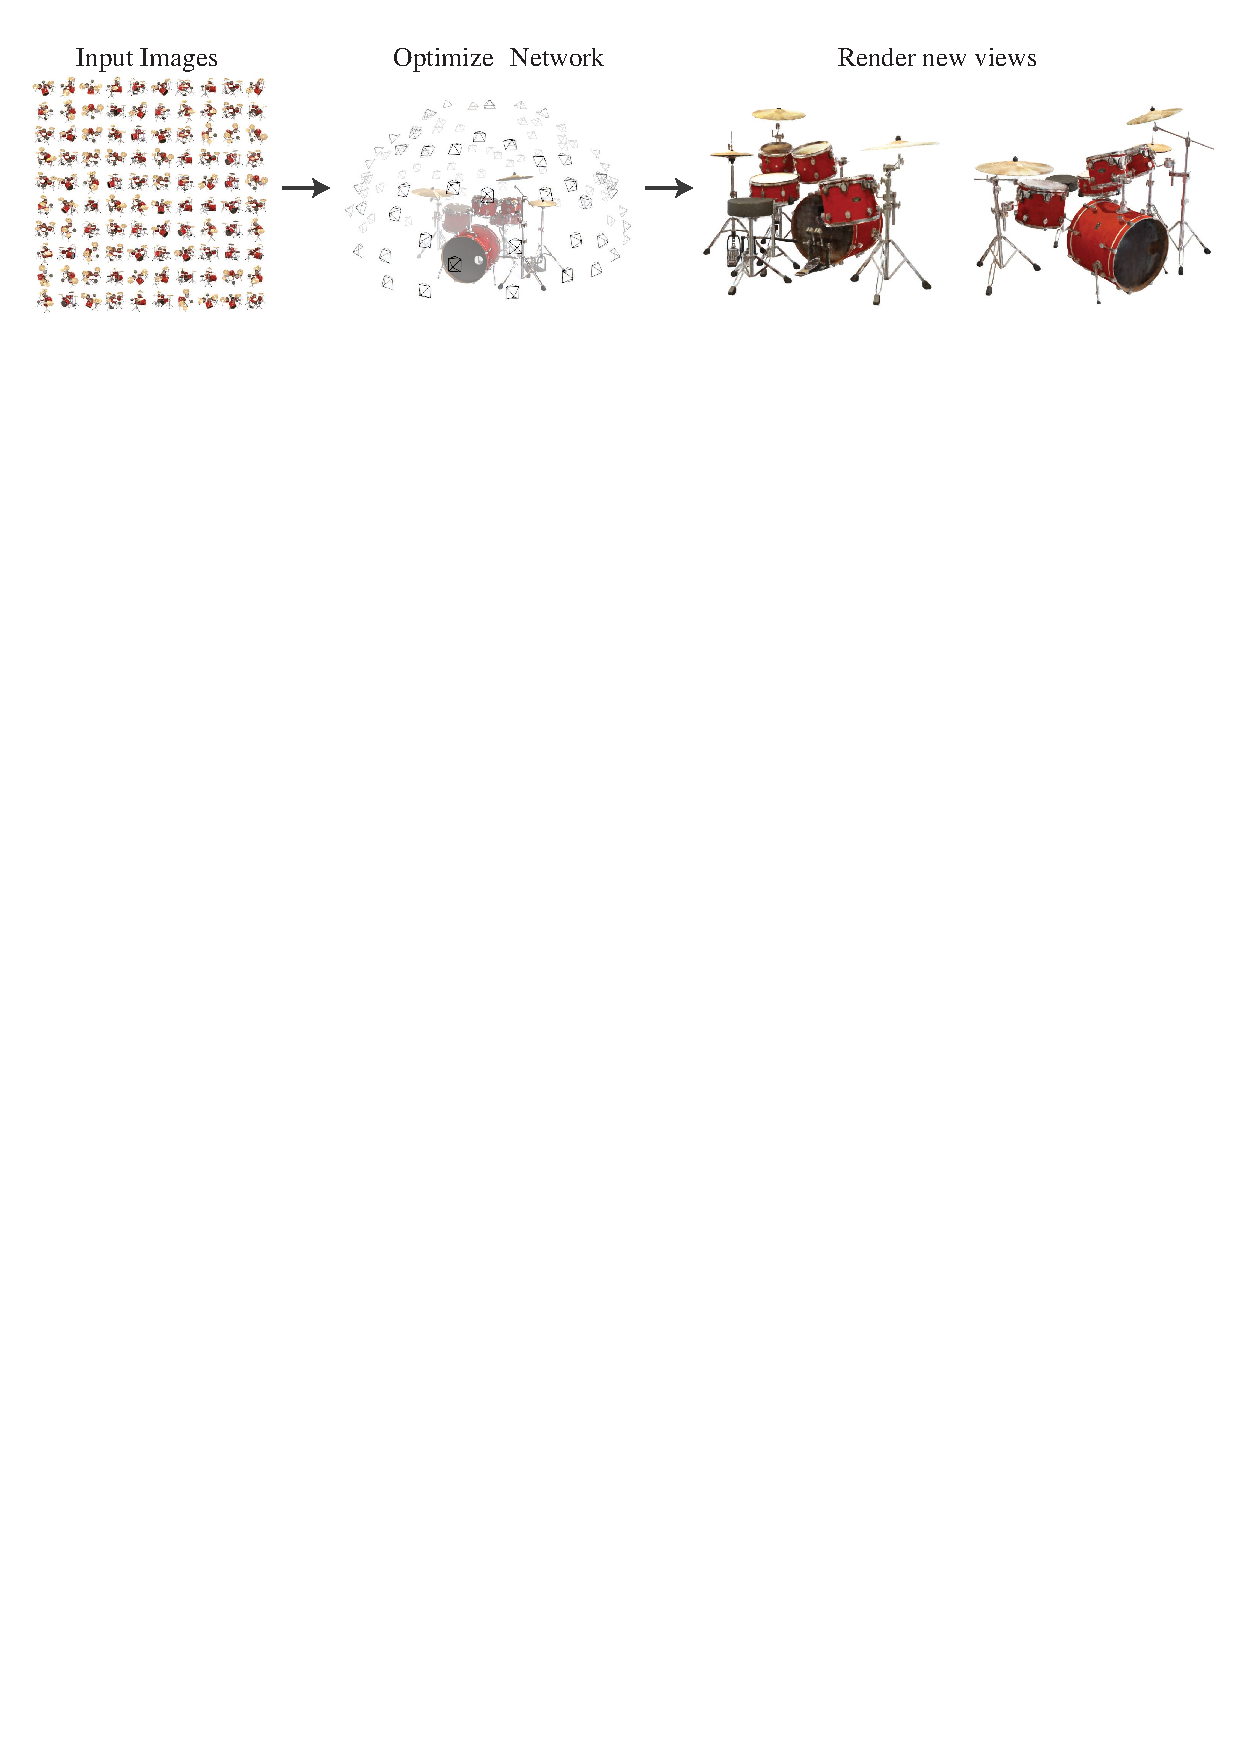
\includegraphics[width=0.95\linewidth]{figures/drums.pdf}
  \caption{新视角合成的过程\cite{mildenhall2020nerf}}
  \label{fig:novelviewsynthesis}
\end{figure}

\section{深度学习发展概述}
深度学习 (Deep Learning, DL) 是机器学习的一个分支,是一种以人工神经网络(如图~\ref{fig:neuralNetwork})为架构进行表征学习的方式。深度学习有着非常悠久的历史,最早可以追溯到20世纪40年代\cite{goodfellow2016deep}。学习可以是有监督的、无监督的,也可以是半监督的。

深度学习发展到现在,得益于 GPU 性能的巨大提升,已有诸如深度神经网络 (Deep Neural Network, DNN) ,深度置信网络\cite{hinton2009deep} (Deep Brief Network, DBN) ,循环神经网络\cite{rumelhart1986learning} (Recurrent Neural Network,RNN) ,卷积神经网络\cite{lecun1995convolutional} (Convolutional Neural Networks, CNN) 等深度学习框架被应用于计算机视觉、语音识别、自然语言处理、音频识别和生物信息学上。

由于本文主要涉及计算机视觉和计算机图形学的知识,因此接下来两小节会介绍这些领域最常用的两个网络架构,卷积神经网络和残差网络 Resnet 。

\begin{figure}[t]
  \centering
  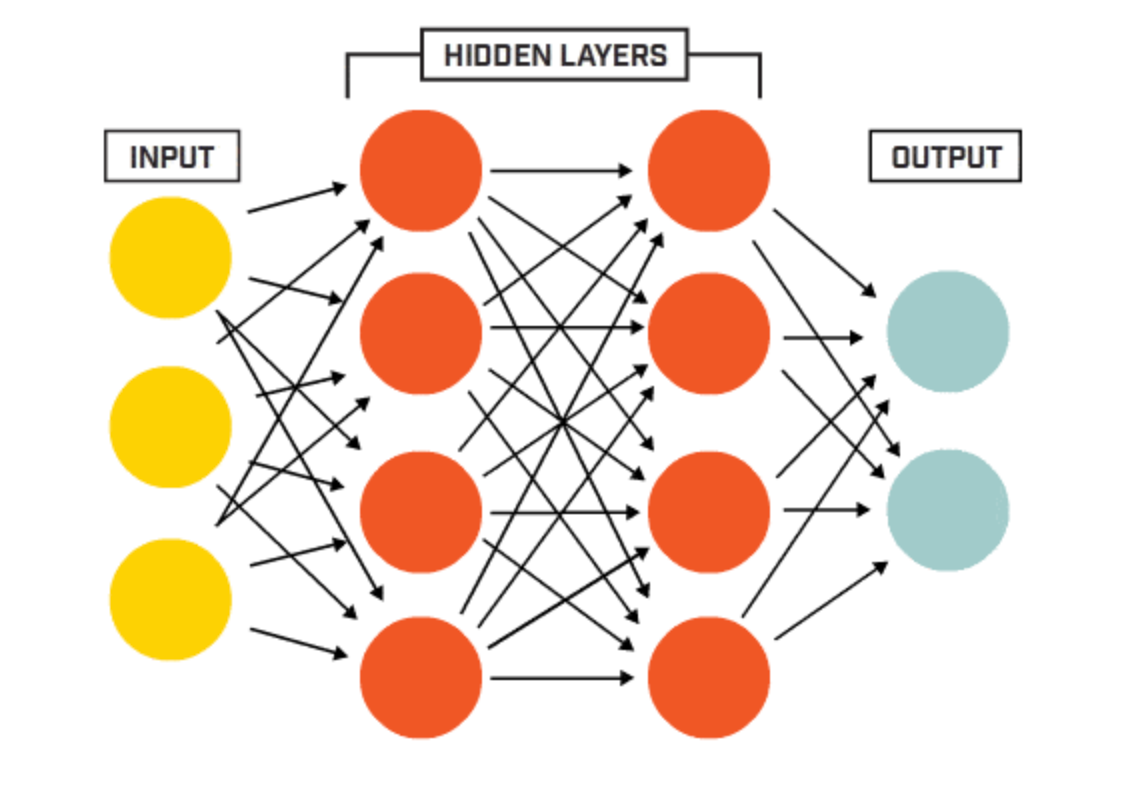
\includegraphics[width=0.9\linewidth]{figures/fc.png}
  \caption{神经网络示意图}
  \label{fig:neuralNetwork}
\end{figure}

\subsection{卷积神经网络}
要具体阐述卷积神经网络,就不得不先提到 MLP ,如图~\ref{fig:neuralNetwork},主要由输入层,隐藏层和输出层三个模块。除了输入层和输出层,隐藏层经常采用 sigmoid 和 tanh 作为激活函数,这里激活函数的作用是为了增加网络非线性拟合能力,若是没有激活函数,即使是使用多层网络进行训练,实际上只相当于一层,只能进行线性拟合,没有很大的作用。不过上述两种激活函数在输入太小或者太大的时候会造成梯度接近于0,这使得梯度更新十分缓慢甚至可能消失,网络从而无法训练下去。与 tanh 相比,sigmoid 还有个非常不利于学习的问题,那就是 sigmoid 函数的值域是$[0,1]$,也因此输出的均值不会为0,这非常不利于下一层的学习。为了解决上述问题,Glorot 等人\cite{glorot2011deep}提出了 ReLU 函数,解决了在输入为正数时梯度消失的问题,此外由于计算比 sigmoid 和 tanh 简单,前向传播和反向传播也都相应更快。

对于正向传播,$l$层的输出和$l-1$层的关系始终可以由下列公式来表达,而与网络深度无关。
\begin{equation}
    a^{l} = \sigma(z^{l}) = \sigma(f(a^{l-1})),
\end{equation}
其中$z^l = f(a^{l-1})$,$f$表示第$l$层网络对应的映射函数,$a^{l-1}$表示前一层的输出(也是第$l$层的输入,$\sigma$表示激活函数)。而反向传播则可用链式法则来进行每一层的求导,计算出梯度。

但是对于图像这种数据来说,全连接网络有着很大的问题,一方面,比如即便是$256 \times 256 \times 3$这样的小图像也需要数十万的参数,这么多参数会使得网络的训练难以进行下去;另一方面,图像数据不像其他任务中的数据,图像本身具有一定的高级语义,为了更好处理地处理像图像这样的二维数据,卷积神经网络应运而生。CNN是一种前馈神经网络,由一个或多个卷积层和顶端的全连接层(对应经典的神经网络)组成,同时也包括共享参数和池化层。这一结构使得卷积神经网络能够利用输入数据的二维结构。这一模型也可以使用反向传播算法\cite{rumelhart1986learning}进行训练。相比较其他深度、前馈神经网络,卷积神经网络需要考量的参数更少,使之成为一种颇具吸引力的深度学习结构。

\begin{enumerate}
    \item 卷积层 \\
    卷积层的功能实际上是对输入进行特征提取。卷积层一般会包含多个神经元,或者叫做卷积核,组成卷积核的每一个元素都会包含一个权重和一个偏移量 (Bias Vector)。卷积核在工作的时候会有规则的扫过输入的特征,对卷积核大小范围内的特征做矩阵乘法并求和,最后再叠加上偏移量。
    
    对一张二维图像$X$,卷积层的输出可表示为
    \begin{equation}
        y_{ij} = \sum_{u=1}^{m}\sum_{v=1}^{n}w_{uv} * x_{i-u+1,j-v+1},
    \end{equation}
    其中$x$表示输入图像$X\in{R^{M\times N}}$的一个像素大小,$w$是卷积核$W \in R^{m\times n}$的参数,一般地$m << M$,$n << N$。
    二维卷积的示意图如图~\ref{fig:2dconv}
    \begin{figure}[htbp]
        \centering
        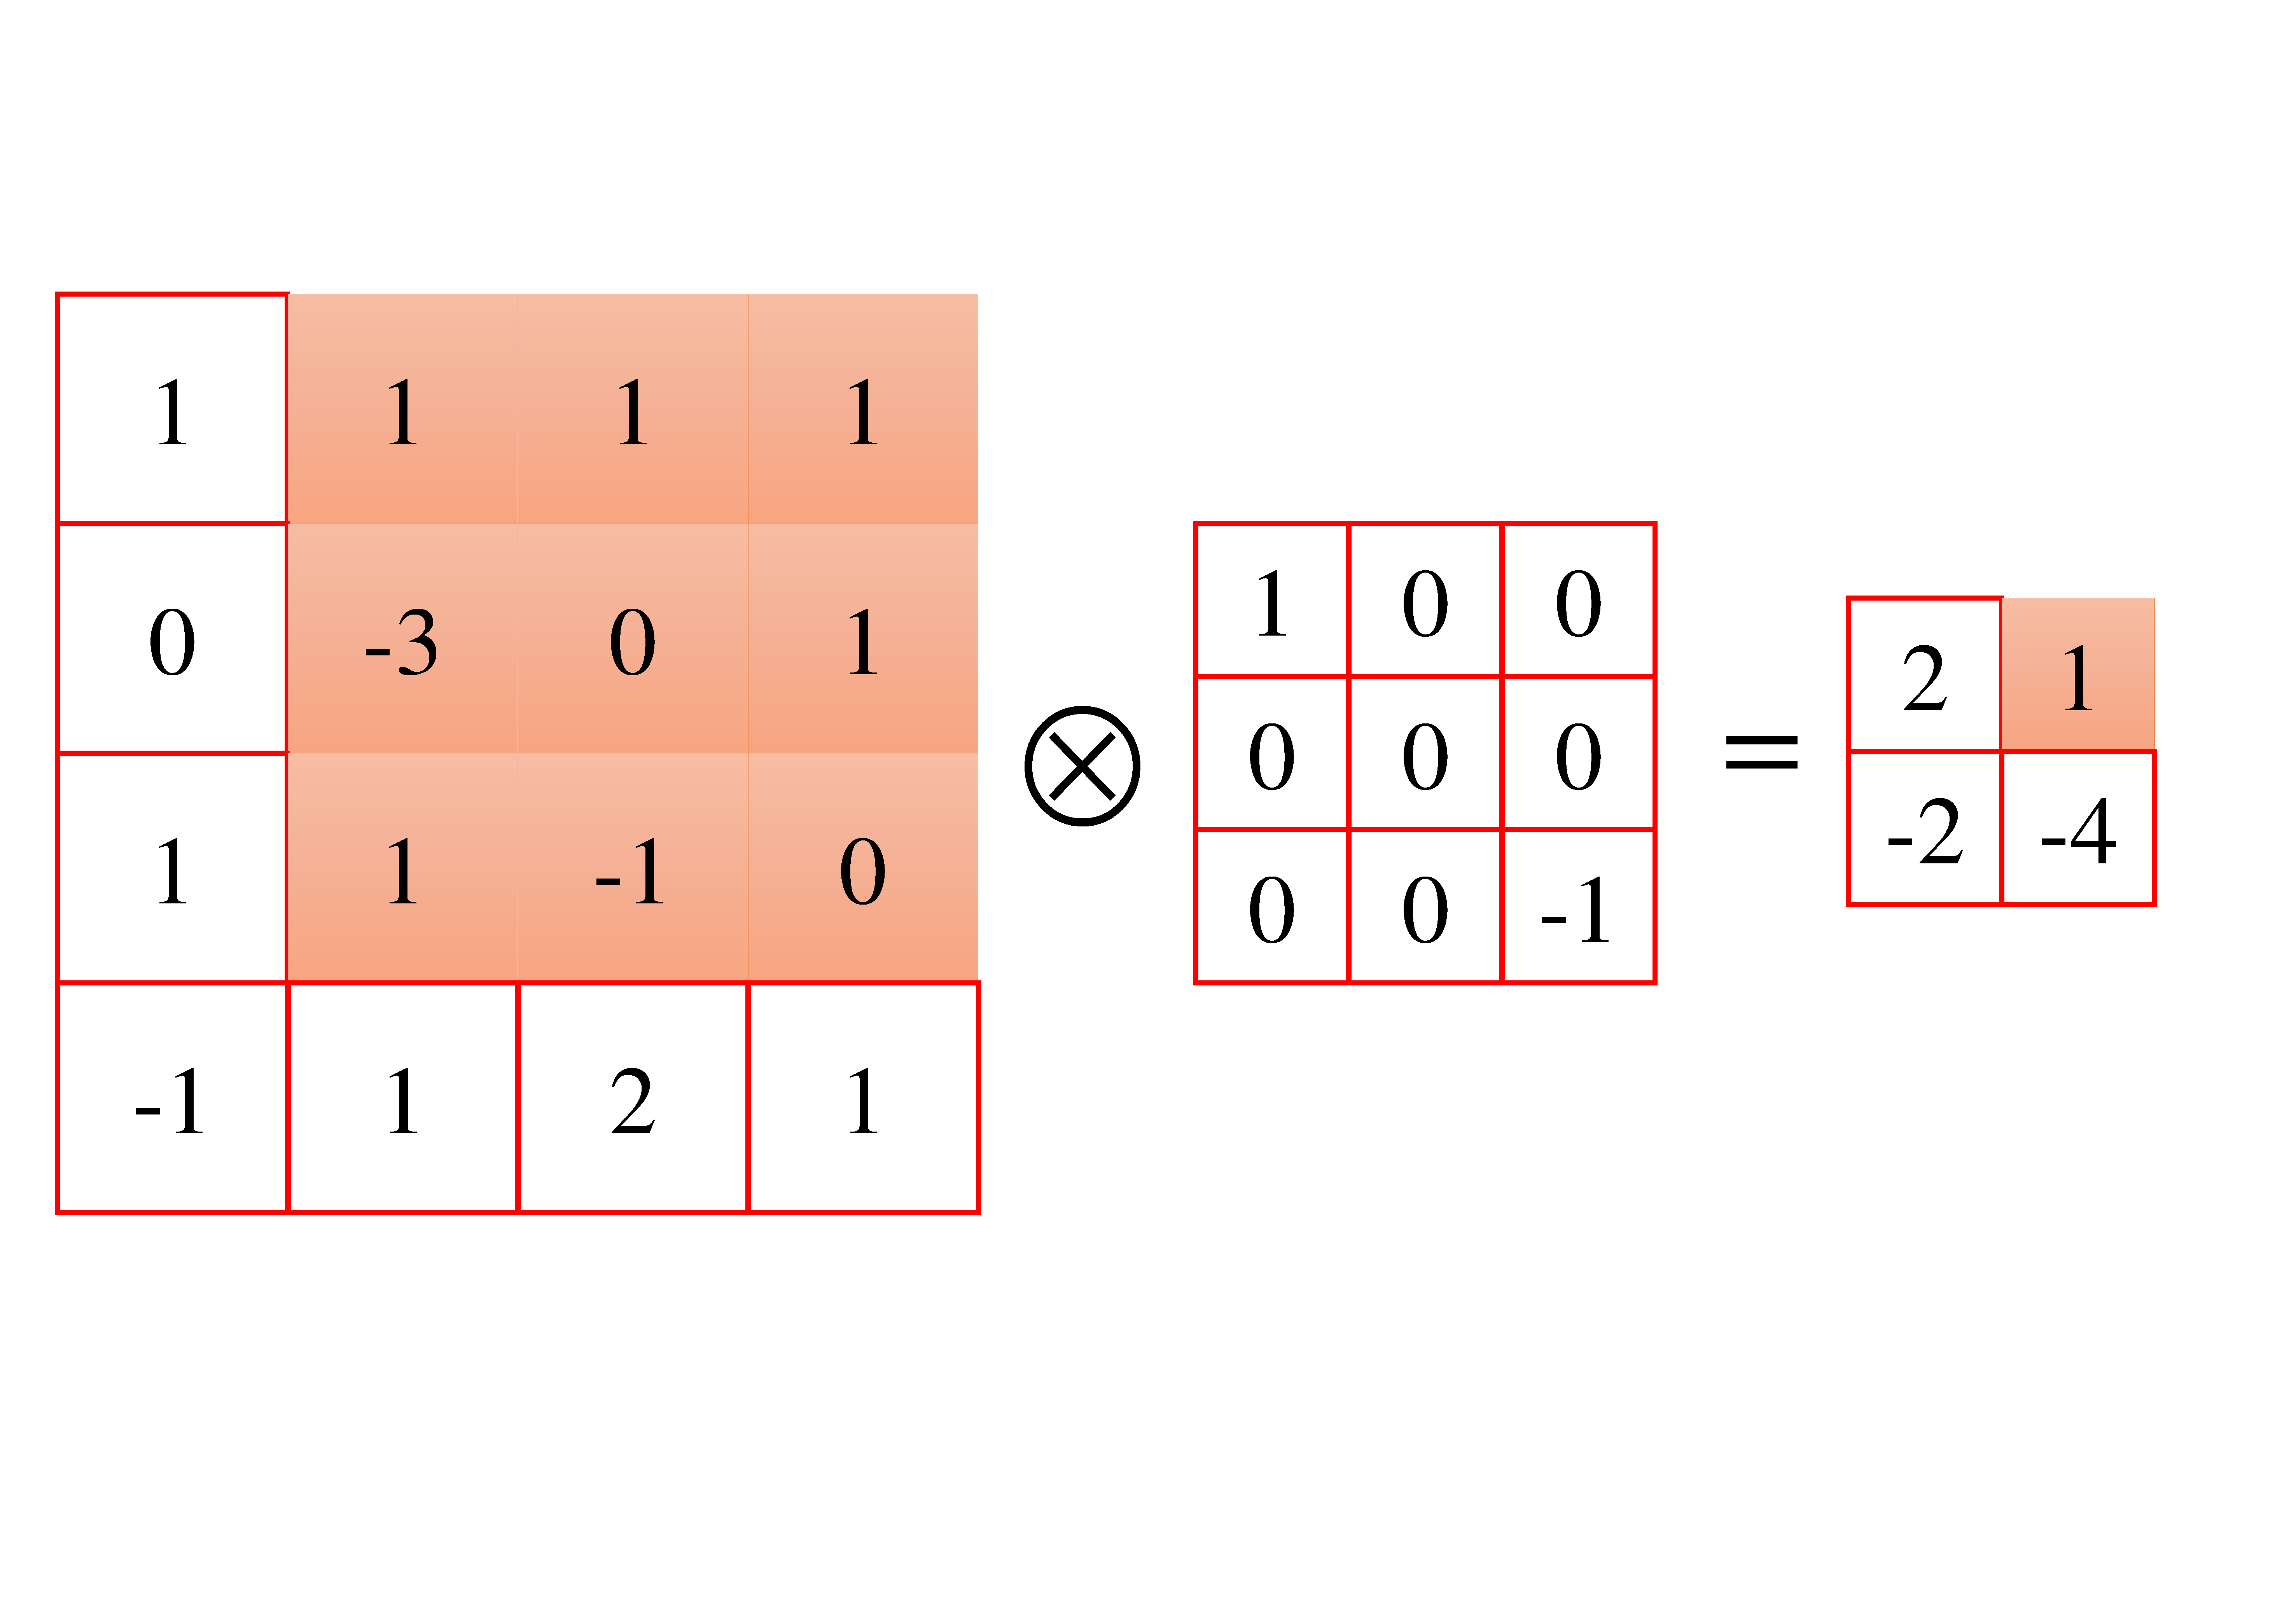
\includegraphics[width=0.7\linewidth]{figures/2dconv.pdf}
        \caption{二维卷积过程}
        \label{fig:2dconv}
    \end{figure}
    \item 池化层 \\
    池化层可以理解为下采样,减少输出特征的尺寸,能扩大感受野还能减少参数。最大池化和平均池化是最常见的两种方法。一般卷积层后会配合一个池化层,能进一步提取到有效的特征,保留主要特征并减少参数。
    \item 全连接层 \\
    无论说是一般的深度学习网络还是 CNN 这样稍微复杂的网络,全连接层都是关键所在。对于 MLP 这样的网络,那么就只有全连接层,可见全连接层的重要性。而对于卷积神经网络而言,全连接层就是将卷积层和池化层提取到的特征整合并输出预测结果。
\end{enumerate}

卷积层的提出极大地促进了计算机视觉领域的发展,AlexNet\cite{2012ImageNet} (5层卷积层、3层全连接层)在2012年的ImageNet视觉识别挑战赛中斩获冠军,可见CNN对于图像这样高级语义任务的巨大能力。此后,VGG\cite{simonyan2014very} 网络改进了 AlexNet 的网络,使得整个网络更深(19层),这使他成为了2014年 ImageNet 挑战赛的第一名。随着 VGG 的提出,人们开始倾向把网络加深,期望获得更好的识别效果。但实际上随着网络的逐渐加深,更深的网络难以训练,出现了因网络太深导致模型退化的问题,这是由于层数越深,训练误差越大,这与深度神经网络的初衷是背道而驰的,也不符合神经网络拟合任意复杂函数的理论。

但是众所周知的是,深度神经网络并没有消失在人们的视野里,这是由于残差网络 Resnet 的出现,这会在下一节进行具体介绍。
\subsection{残差网络 Resnet}
Kaiming He 等人借鉴了 Highway Network\cite{srivastava2015highway} 的跨层连接思想,并提出了赫赫有名的残差网络 Resnet\cite{he2016deep} ,较好地解决了当神经网络极深时模型失效无法训练的问题,并且在当时的 ImageNet 大赛上获得了第一名的好成绩。本文使用的神经辐射场的网络是基于残差模块设计的,因此接下来详细介绍残差网络的设计想法。

如图~\ref{fig:resnet}所示,经典的残差网络由多个残差模块组成,因此可以根据需求自行设计网络的深度。残差网络核心思想是使用了 shortcut 这一操作,即将输入传到输出作为输出的一部分,用公式表达就是$H(x) = F(x) + x$,当$H(x) = x$时为恒等映射,这里的$F(x)$就是需要学习的残差。这样的设计原理是,当深度学习网络极深的时候,由于训练误差较大,无法提取出更抽象的特征,那么此时有了这样的残差结构,就可以学习到一个恒等映射,至少还能保留前面提取出的特征。虽然学习一个恒等映射不是非常容易,不过由于 shortcut 这一操作使得只需让残差往0的方向去学习即可,这样也同时有效避免了梯度消失的问题。resnet 的出现是具有划时代的意义的,它解决了极深的神经网络难以训练的问题,通过有效地学习到恒等映射来保证当网络越来越深的时候所导致的模型退化性能衰退的情况。

本文的基础网络架构就是引入了 skip connection(或者是上述的 shortcut )的操作来将输入的特征往网络深处传送,以此来训练出一个高质量的深度学习网络,这样才能学习到细粒度的连续的神经辐射场。
,
\begin{figure}[t]
    \centering
    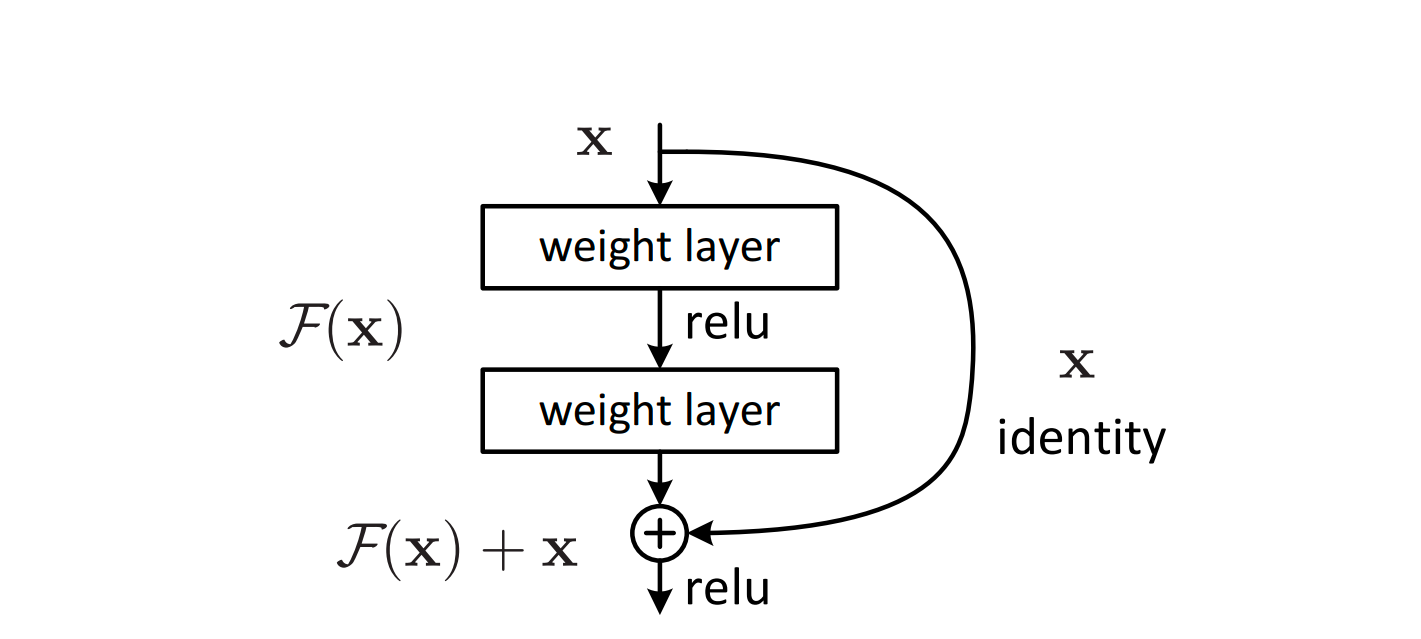
\includegraphics[width=0.7\linewidth]{figures/resnet.jpg}
    \caption{典型的残差结构}
    \label{fig:resnet}
\end{figure}

\section{查询表的加速方法}
在计算机科学中,查询表 (Lookup Table) 一般是一种简单的数组结构,通过简单的数组索引操作替代一些复杂的计算。一般来说,查询表的加速是很可观的,因为直接从内存中提取到相关数据往往要比复杂的计算快很多。

%一个经典的例子就是三角函数表。每次计算所需的正弦值在一些应用中可能会慢得无法忍受,为了避免这种情况,应用程序可以在刚开始的一段时间计算一定数量的角度的正弦值,譬如计算每个整数角度的正弦值,在后面的程序需要正弦值的时候,使用查找表从内存中提取临近角度的正弦值而不是使用数学公式进行计算。
一个典型的应用场景是自然对数表,在一些应用中,直接计算自然对数值是难以接受的,为了解决这一问题,可以提前将一些常用值的自然对数缓存在查询表中,在计算未知的对数值的时候,可以通过直接查询临近值的对数值而避免了复杂的数学计算,这大大加快了计算效率。

%一些折衷的方法是同时使用查找表和插值这样需要少许计算量的方法,这种方法对于两个预计算的值之间的部分能够提供更高的精度,这样稍微地增加了计算量但是大幅度地提高了应用程序所需的精度。根据预先计算的数值,这种方法在保持同样精度的前提下也减小了查找表的尺寸。

在一些细粒度的任务中,往往需要获得较高精度的查询结果,这时候就需要进行一些折衷,比如在使用查询表的同时结合插值的方法,通过略微增加计算量的方式增加了精度,同时也一定程度减少了查询表的尺寸。

%在图像处理中,查找表将索引号与输出值创建联系。颜色表作为一种普通的 LUT 是用来确定特定图像中每一像素所要显示的颜色和强度。

%另外需要注意的一个问题是,尽管查找表经常效率很高,但是如果所替换的计算相当简单的话就会得不偿失,这不仅仅因为从内存中提取结果需要更多的时间,而且因为它增大了所需的内存并且破坏了高速缓存。如果查找表太大,那么几乎每次访问查找表都会导致高速缓存缺失,这在处理器速度超过内存速度的时候愈发成为一个问题。
值得注意的是,虽然查询表的加速效率一般很高,但是通过查询表替换的计算方式过于简单,那么可能会出现从内存中提取数值的速度低于直接计算的速度,这样就得不偿失。

查询表实质是一种通过空间换时间的方式,但是实际应用中内存是有限的,因此必须要考虑查询表尺寸的问题。

%如何构建查找表有两个基本的约束条件,一个是可用内存的数量;不能构建一个超过能用内存空间的表格,尽管可以构建一个以查找速度为代价的基于磁盘的查找表。另外一个约束条件是初始计算查找表的时间——尽管这项工作不需要经常做,但是如果耗费的时间不可接受,那么也不适合使用查找表。

如图\ref{fig:justlookup}所示,以 justlookup\cite{lin2019justlookup} 为代表的工作拓宽了查询表的使用,justlookup 已经证明了对逐点网络可以去构建查询表来加速网络的前向传播并通过对近似特征再学习的策略来维持模型精度不损失,这一思想也可以应用到本文的模型加速上,通过查询表缓存网络参数,以此替换掉一些全连接层,这样可以少经过一些网络而直接通过查询表查询到中间层网络特征,从而加速前向传播。查询表技术在本文的具体应用详见下一章。

\begin{figure}[t]
    \centering
    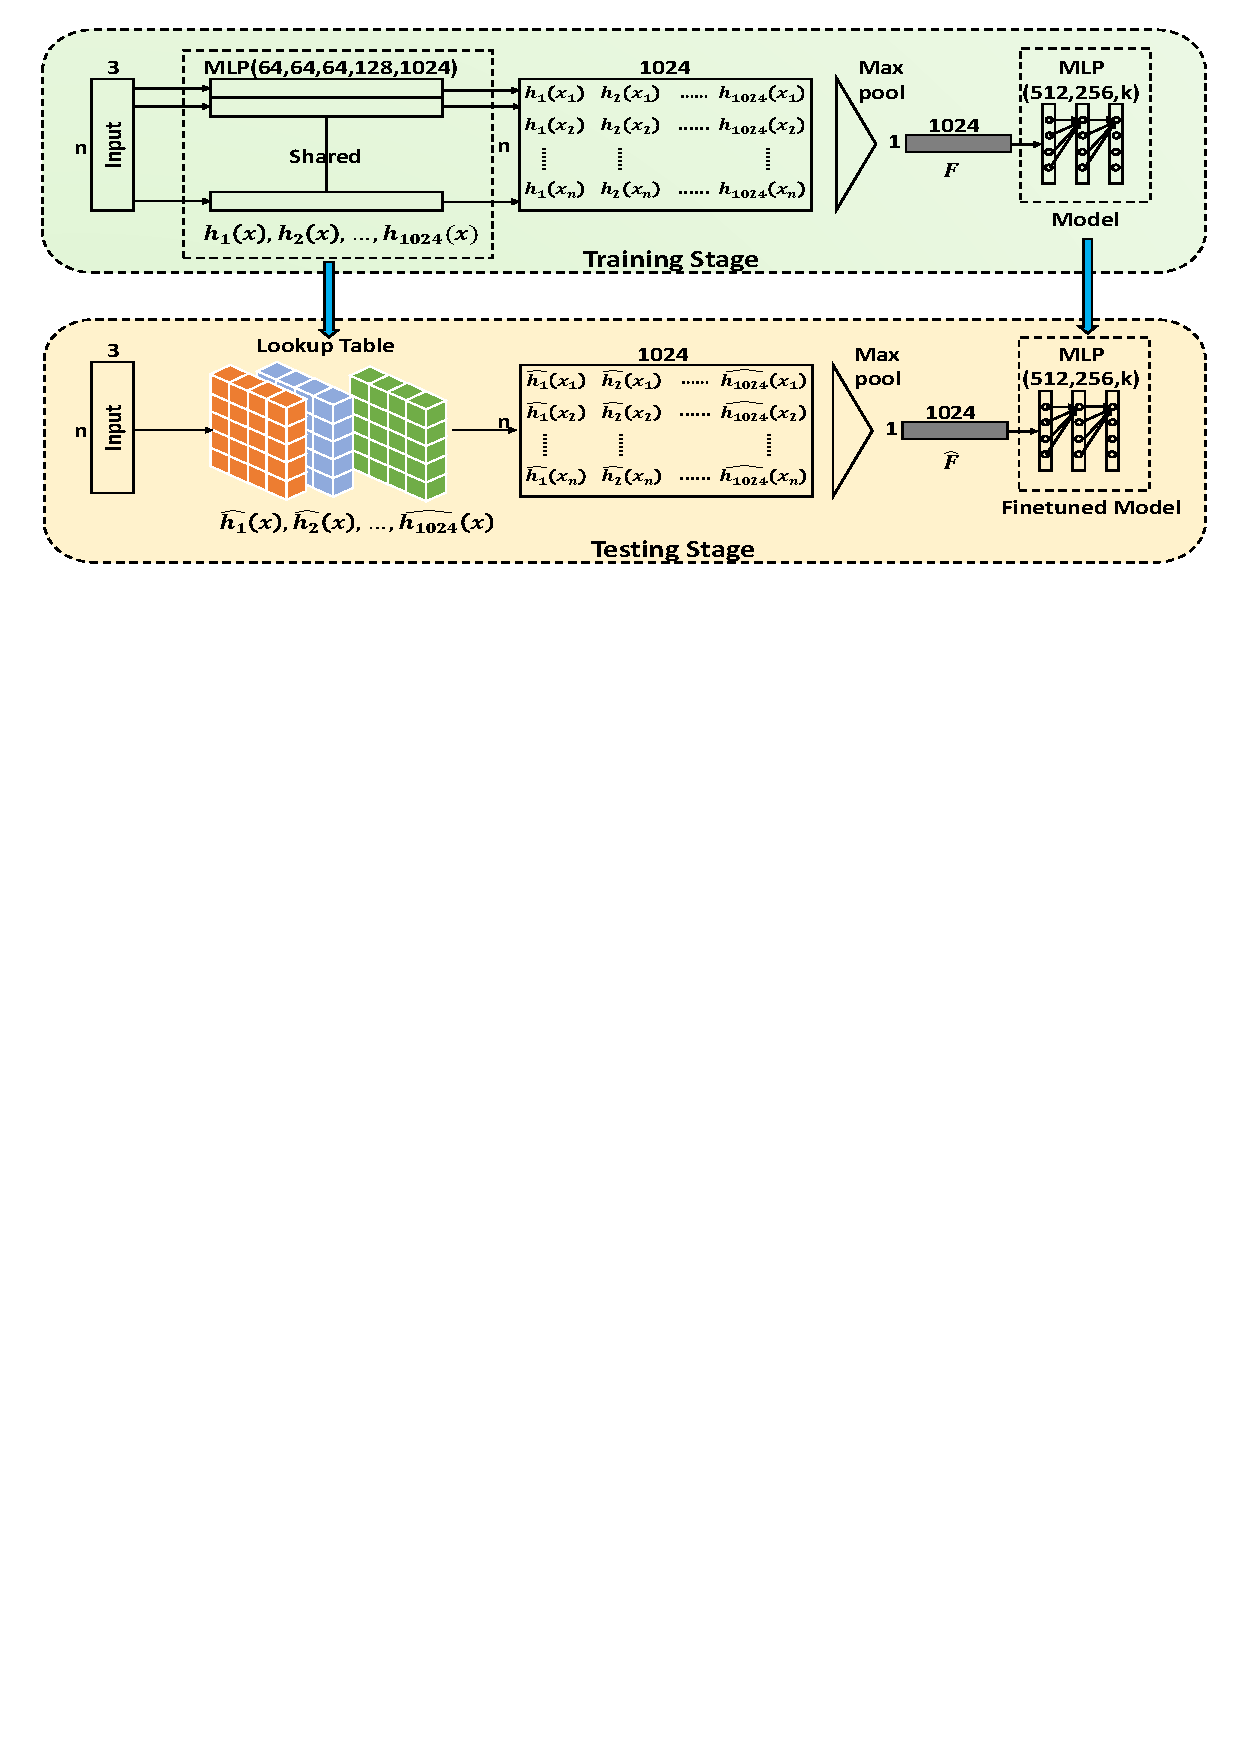
\includegraphics[width=0.9\linewidth]{figures/justlookup.pdf}
    \caption{查询表在逐点网络上的应用\cite{lin2019justlookup}}
    \label{fig:justlookup}
\end{figure}


\section{本章小结}
本章介绍了与本文研究技术相关的一些技术以及理论,包含用于描述 3D 形状的一些表示方法,以及与本文任务最相关的新视图合成和基于图像的渲染,还有关于深度学习的一些基础概念,这些都构成了本文方法的基础。最后介绍了关于查询表的加速方法,以及将其应用到含有逐点网络的前向传播上的经典方法,这一思路也成为了本文方法的根基,将在下一章节详细阐述本文的方法。

\cleardoublepage
% !TeX root = ../main.tex

\chapter{本文提出的方法}\label{citations}
上一章对本文研究相关的神经辐射场应用于新视图合成的相关原理和技术进行了概述。本文的研究始终围绕着“基于神经辐射场的新视图合成加速”这一框架展开。本章主要详细介绍本文的方法论部分,包含问题的定义,NeRF 的相关预备理论,以及本文提出的对 NeRF 加速的具体方法,最后是对本章的总结。

\section{问题定义}
本节将简要阐述本文所研究的问题定义。
首先本文的研究目标是基于移动端三维传感器采集的物体的不同视角的图像,快速渲染推理出新视角下的图像。要达到上述目标需要解决NeRF网络中如下的几个问题:
\begin{enumerate}
    \item 由于新视图合成是细粒度的渲染问题,NeRF 为了获取对渲染图象贡献较高的采样点,在训练和推理的过程中使用 coarse 网络和 fine 网络,通过 coarse 网络的输出来估计体密度随深度的变化分布,然后基于此分布进行二次采样并通过 fine 网络预测的颜色和体密度进行数值积分计算出 2D 图像对应像素的 RGB 值,这样两个网络的前向传播带来的开销是比较大的。
    \item NeRF 使用了深度学习网络,网络中较多的全连接层,尤其是该网络本质上是逐点网络,这对加速渲染过程来说也是能够优化的部分。
\end{enumerate}

\section{新视图合成的神经辐射场表示}
新视图合成的目的是基于已有的视角的图像,推理未知视角下的图像,现有的基于神经辐射场的体绘制方法已经可以合成较高质量的新视角图像。本节详细介绍神经辐射场 NeRF 的主要方法,包含神经辐射场的场景表示,基于神经辐射场的立体渲染,神经辐射场的优化三部分,由 NeRF 的方法论给本文提供一定的问题来源和理论支撑。

\begin{figure}[htbp]
    \centering
    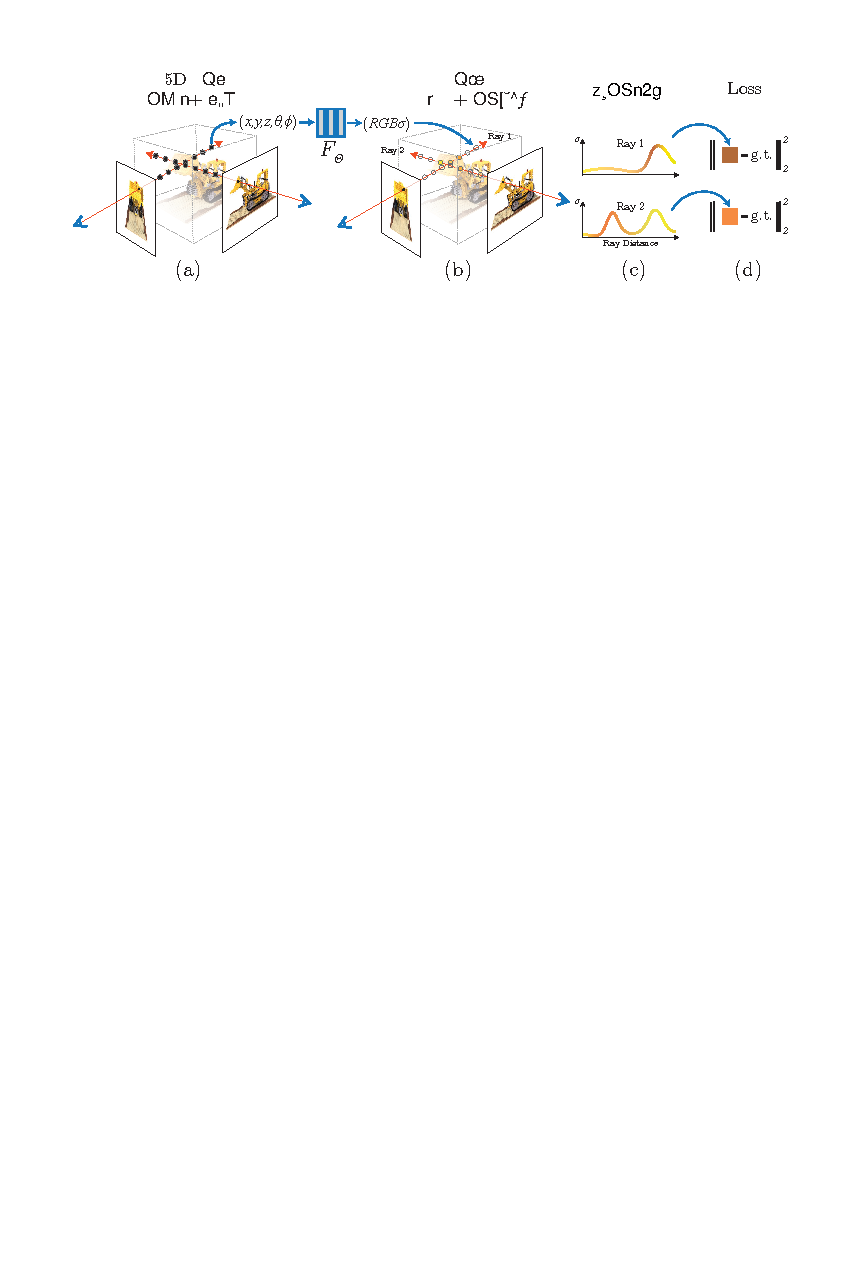
\includegraphics[width=0.95\linewidth]{figures/nerf_io.pdf}
    \caption{神经辐射场的场景表示和可微的渲染过程概况\cite{mildenhall2020nerf}。(a) 沿着相机光线采样 5D 坐标(位置和观测方向);(b) 将 (a) 中位置馈入 MLP 以生成颜色和体密度;(c) 将 (b) 中的这些输出使用立体渲染的方法合成相应的图像;(d) 此渲染过程是可微的,因此可以通过最小化合成的和 ground truth 观测图像之间的残差来优化场景表示}
    \label{fig:nerf_io}
\end{figure}

\subsection{神经辐射场的场景表示}
NeRF 的整体框架是使用 5D 的向量值函数来表示连续的场景,其中,输入是一个 3D 坐标$\displaystyle \symbf{x} = \left(x, y, z \right)$ 和 2D 的视角方向 $\displaystyle \left(\theta, \phi \right)$,输出是NeRF 的整体框架是使用 5D 的向量值函数来表示连续的场景,其中,输入是一个 3D 坐标$\displaystyle \symbf{x} = \left(x, y, z \right)$ 和 2D 的视角方向 $\displaystyle \left(\theta, \phi \right)$,输出是发出的颜色$\displaystyle \symbf{c} = \left(r, g, b \right)$和体密度$\displaystyle \sigma$。实际上,方向被表示为三维直角坐标系中的单位向量$\displaystyle \symbf{d}$。NeRF 通过 MLP 网络$\displaystyle F_{\Theta} : \left(\symbf{x}, \symbf{d} \right) \Rightarrow \left(\symbf{c}, \sigma \right)$ 来估计这个连续的 5D 场景表示,并优化网络权重 $\displaystyle \Theta$ ,建立起 5D 坐标到相应的体密度以及方向发出颜色的映射。

\subsection{基于神经辐射场的立体渲染}
NeRF 的 5D 神经辐射场将场景表示为空间内任意一点的体密度和定向发出的辐射,并且使用经典体积渲染的原理来渲染穿过场景的任何光线的颜色。体积密度$\displaystyle \sigma \left(\symbf{x} \right)$可以解释为一条光线在$\displaystyle \symbf{x}$的位置处终止于无穷小粒子的概率。相机光线$\displaystyle \symbf{r}\left(t \right) = \symbf{o} + t \symbf{d}$在近远界限分别为$\displaystyle t_n$和$\displaystyle t_f$时所对应的颜色的期望为:
\begin{equation}
    C \left(\symbf{r} \right) = \int_{t_n}^{t_f}T\left(t\right)\sigma\left(\symbf{r}\left(t\right)\right)\symbf{c}\left(\symbf{r}\left(t\right), \symbf{d}\right)dt, 
    \mbox{其中}T\left(t\right) = \exp \left(-\int_{t_n}^{t}\sigma\left(\symbf{r}\left(s\right)\right)ds\right).
\end{equation}
$\displaystyle T\left(t\right)$表示沿光线从$t_n$到$t$的累积透射率,即$t_n$到$t$光线没有碰到任何粒子的概率。从连续的神经辐射场中渲染一个视角需要估计通过所需虚拟相机的每个像素跟踪的相机射线的积分$\displaystyle C\left(\symbf{r}\right)$。

计算机是无法计算连续积分的,因此需要用到数值估计,利用求面积法来估计连续积分。 确定性求面积通常用于渲染离散体素网格,将有效地限制所表示的分辨率,因为 MLP 仅在固定的离散位置上查询。 相反,NeRF 使用分层抽样方法对$\displaystyle \left[t_n, t_f\right]$放入$N$个均匀分布的容器中,然后从每个容器中随机抽取一个样本:
\begin{equation}
    t_i \sim \mathcal{U} \left[t_n + \frac{i - 1}{N}\left(t_f - t_n\right), t_n + \frac{i}{N}\left(t_f - t_n\right) \right].
    \label{eq:uniform}
\end{equation}
虽然使用的是离散的样本集去估计积分,但是分层采样使的能表示连续的场景,这是因为它使的 MLP 在优化过程中在连续的位置进行评估。 最终是通过这些样本来估计$C(r)$。
\begin{equation}
    \hat{C}\left(\symbf{r}\right)=\sum_{i=1}^{N}T_i\left(1-\exp\left(-\sigma_i\delta_i\right)\right)\symbf{c}_i, \mbox{其中}T_i=\exp\left(-\sum_{j=1}^{i-1}\sigma_j\delta_j \right),
    \label{eq:getcolor}
\end{equation}
$\displaystyle \delta_i = t_{i + 1} - t_i$是相邻两个采样点的距离。这个函数对于计算$\displaystyle \hat{C}\left(\symbf{r}\right)$的一组$\displaystyle \left(\symbf{c}_i, \sigma_i\right)$值是可微的,使用 alpha 值 $\displaystyle \alpha_i = 1 - \exp \left(-\sigma_i\delta_i\right)$ 来简化成传统的 alpha 合成。 

\subsection{神经辐射场的优化}
上一节描述了将场景建模为神经辐射场并从该表示渲染新视图所必需的核心组件。 但是,NeRF注意到这些组件不足以实现更高质量。NeRF介绍了两项改进,以此表示高分辨率的复杂场景。 第一种是输入坐标的位置编码,可帮助MLP表示高频函数,第二种是分层采样过程,可让有效地采样此高频表示。

\subsubsection{位置编码}
尽管理论上神经网络可以拟合任何函数,但是 NeRF 发现直接向网络$\displaystyle F_{\Theta}$中输入$\displaystyle xyz\theta\phi$会使的渲染效果不是非常好,在颜色和几何的高频变化上表现的非常差。这与 Rahaman 等人\cite{rahaman2019spectral}最近的工作是一致的,该工作表明深度网络倾向于学习低频函数。他们还表明,在将输入传递到网络之前,使用高频函数将输入映射到更高维度的空间可以更好地拟合包含高频变化的数据。

在神经场景表示的背景下利用上述发现,把$\displaystyle F_{\Theta}$重构成一个由两个函数组成的复合函数$\displaystyle F_{\Theta} = F_{\Theta}^{\prime} \circ \gamma$,一个是学习的,另一个则是已知的,这能够明显地提升质量表现。$\displaystyle \gamma$建立了$\displaystyle \mathbb{R}$到更高维空间$\displaystyle \mathbb{R}^{2L}$的映射,$\displaystyle F_{\Theta}^{\prime}$仍是一个常规的 MLP。正式使用的编码函数如下:
\begin{equation}
    \gamma\left(p\right) = \left(\sin\left(2^{0}\pi p\right), \cos\left(2^{0}\pi p\right), \cdots, \sin\left(2^{L - 1}\pi p\right), \cos\left(2^{L - 1}\pi p\right)\right).
\end{equation}
$\displaystyle \gamma\left(\cdot\right)$函数被应用在$\displaystyle \symbf{x}$视角方向的单位向量$\displaystyle \symbf{d}$的每一个坐标值。

\subsubsection{分层体积采样}
接下来介绍一下 NeRF 中最核心的部分,分层体积采样。密集地评估沿着每条相机光线的$N$个查询点的神经辐射场网络的渲染策略效率低下:自由空间和对渲染图像无贡献的遮挡区域仍会被重复采样。 NeRF 从体绘制中的早期工作\cite{levoy1990efficient}中汲取灵感,并提出一种分层表示,通过按比例分配样本到最终渲染的预期效果来提高渲染效率。

NeRF 同时优化两个神经网络:一个是 coarse 网络,另一个是 fine 网络。首先使用分层采样采集一组有$N_c$个位置的样本,在这些位置使用公式~\ref{eq:uniform}和公式~\ref{eq:getcolor}来评估 coarse 网络。基于这个 coarse 网络的输出,就可以沿着每条光线对点进行更准确的采样,其中样本偏向体积的相关部分。为此,首先将~\ref{eq:getcolor}中的 coarse 网络$\displaystyle \hat{C}_{c} \left(\symbf{r}\right)$的alpha合成颜色重写为沿射线的所有采样颜色$\displaystyle c_i$的加权和:
\begin{equation}
    \hat{C}_{c}\left(\symbf{r}\right) = \sum_{i=1}^{N_c}w_{i}c_{i}, w_{i} = T_{i}\left(1 - \exp \left(-\sigma_{i}\delta_{i}\right)\right).
    \label{eq:weight}
\end{equation}
将上述权重进行归一化$\displaystyle \hat{w}_{i} = \frac{w_i}{\sum_{j=1}^{N_c}w_j}$可以生成一个沿着相机光线分段常数的概率密度函数。我们使用逆变换采样从该分布中采样第二组$\displaystyle N_f$个位置,最终使用公式~\ref{eq:getcolor}来计算最终沿着光线渲染的颜色,但是是使用所有$\displaystyle N_c + N_f$个采样点。

由于优化的是两个网络,因此整个 NeRF 的 loss 可以表示为:
\begin{equation}
    \mathcal{L} = \sum_{\symbf{r}\in \mathcal{R}}\left[\left\|\hat{C}_{c}\left(\symbf{r}\right) - C\left(\symbf{r}\right)\right\|_{2}^{2} + \left\|\hat{C}_{f}\left(\symbf{r}\right) - C\left(\symbf{r}\right)\right\|_{2}^{2} \right].
    \label{eq:nerf_loss}
\end{equation}
这个也是本文的动机 (motivation),通过构思,优化采样结构,使之可以减少训练一个网络,这是本文最核心的地方。

\section{基于神经辐射场的新视图合成加速方法}\label{method}
针对 NeRF 采用分层抽样这一做法,即同时优化 coarse 网络和 fine 网络,通过 coarse 网络的输出去估计公式~\ref{eq:weight}中的权重$\displaystyle w_i$的分布情况,生成一个分段常数的概率密度函数,这在 NeRF 中证明是能显著提升渲染质量的。但也正是由于增加了一个网络,那么在网络前向传播这一部分的开销增加了一倍,这在实际应用中是难以接受的。为此,我们将此问题看作是一个领域知识的优化的问题。我们的目标是无论是训练还是在测试过程中,只使用一个网络,这样理论上渲染一张新视图的时间会缩短一半。但是,在 NeRF 中证明了单纯地去减少一个网络势必会降低新视图渲染的质量,因此我们必须采取一定的方式去补偿减少一个网络带来的质量下降。接下来我们首先会介绍本文提出的一个最基本的加速优化模型;然后详细介绍该模型中的核心部分查询表的构建,其中包含网络架构和如何建立起索引的;

\subsection{模型综述}
本小节将详细介绍本文提出模型的设计方法和细节。
\begin{figure}[t]
    \centering
    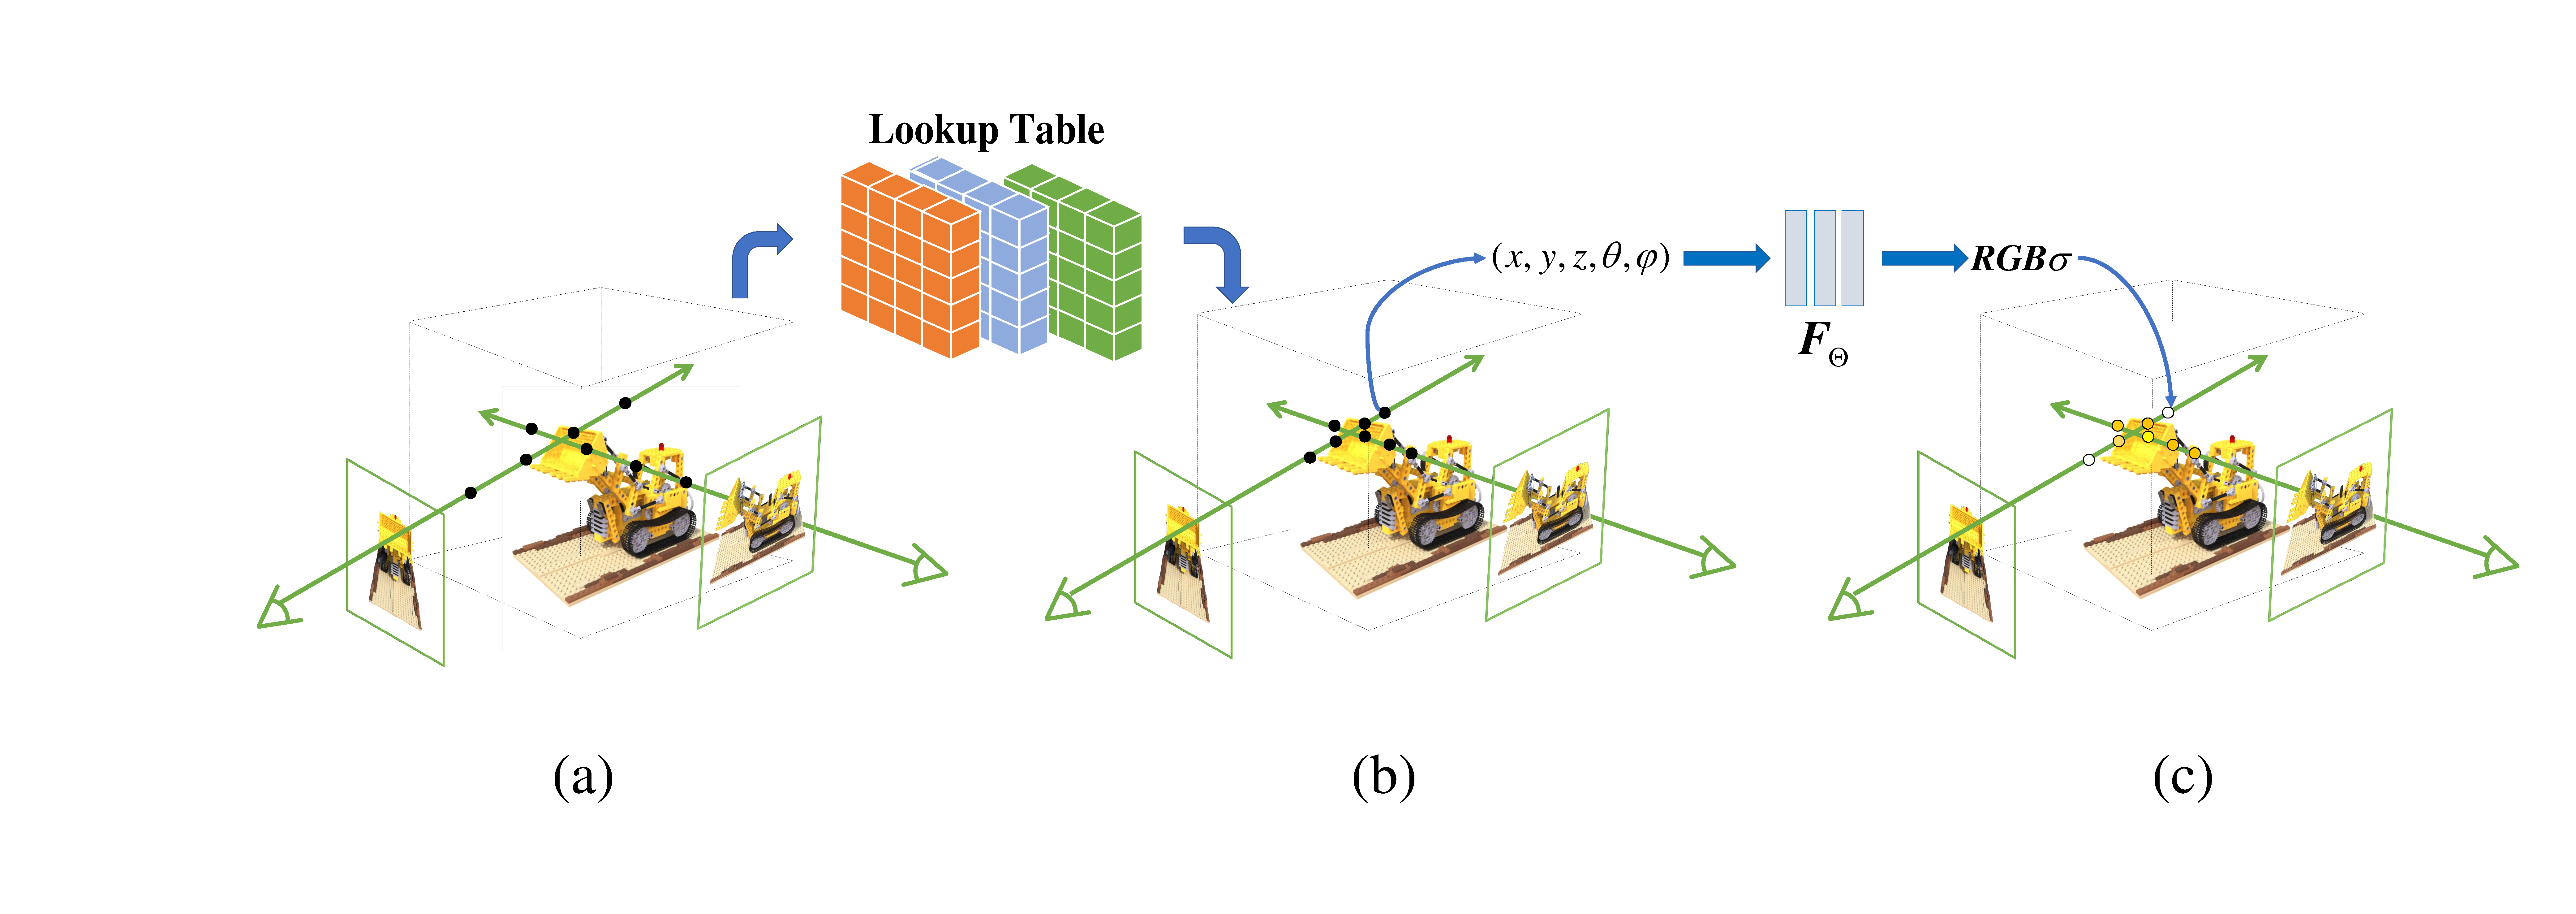
\includegraphics[width=0.95\textwidth, height=0.25\textheight]{figures/fnerf.pdf}
    \caption{神经辐射场的新视图合成的加速框架。(a) 沿着相机光线采样 5D 坐标(位置和观测方向);(b) 通过缓存的特征查询表找到采样点中距离表面最近的点,并在此点附近进行二次采样将 (c) 将 (b) 中位置和方向馈入 MLP 以生成颜色和体密度}
    \label{fig:fnerf}
\end{figure}
如图~\ref{fig:fnerf}所示,本文提出了基于神经辐射场的快速合成新视图的框架,为 NeRF 的推理过程进行提速。本文的框架一共包含三个步骤,第一步是网络裁剪,第二步是提取查询表,第三步是优化采样过程。

对于网络裁剪来说,由于 NeRF 是使用了 coarse 网络和 fine 网络来进行分层采样,为了操作方便,本文是去掉了 fine 网络,仅保留 coarse 网络,这显然会降低渲染的质量水平,因此还需要后面两个步骤的操作。对于提取查询表的过程,这里先简单理解为建立了一个立方体网格,将格点坐标输入到 NeRF 预训练好的网络中,根据体密度为正值这一条件筛选出合格的点的坐标,真正存的是网络中间层的特征,查询表表征物体的近似表面,具体的查询表的构建详见下一小节。对于第三步,我们实现采样值的优化是通过查询表完成的,过程的概况为首先将粗采样的采样点(均匀采样完成的)馈入查询表中,若发现光线上所有点均不在查询表内则忽略该条光线,下面是有交集的情况,沿着光线的方向找到相机光线上第一个在查询表内的点,以此点为中心,适当的区间长度进行二次均匀采样,这些采样点即最终的采样点,位于物体表面附近,对渲染贡献较大。之后将采样点馈入 NeRF 原有的网络框架中输出颜色和体密度,通过积分计算出像素的 RGB 值可以和 ground truth 计算出 loss 并反向传播优化整个网络,最后我们就获得了一个能快速合成新视图的网络框架。

\subsection{查询表的构建}
\begin{figure}[t]
    \centering
    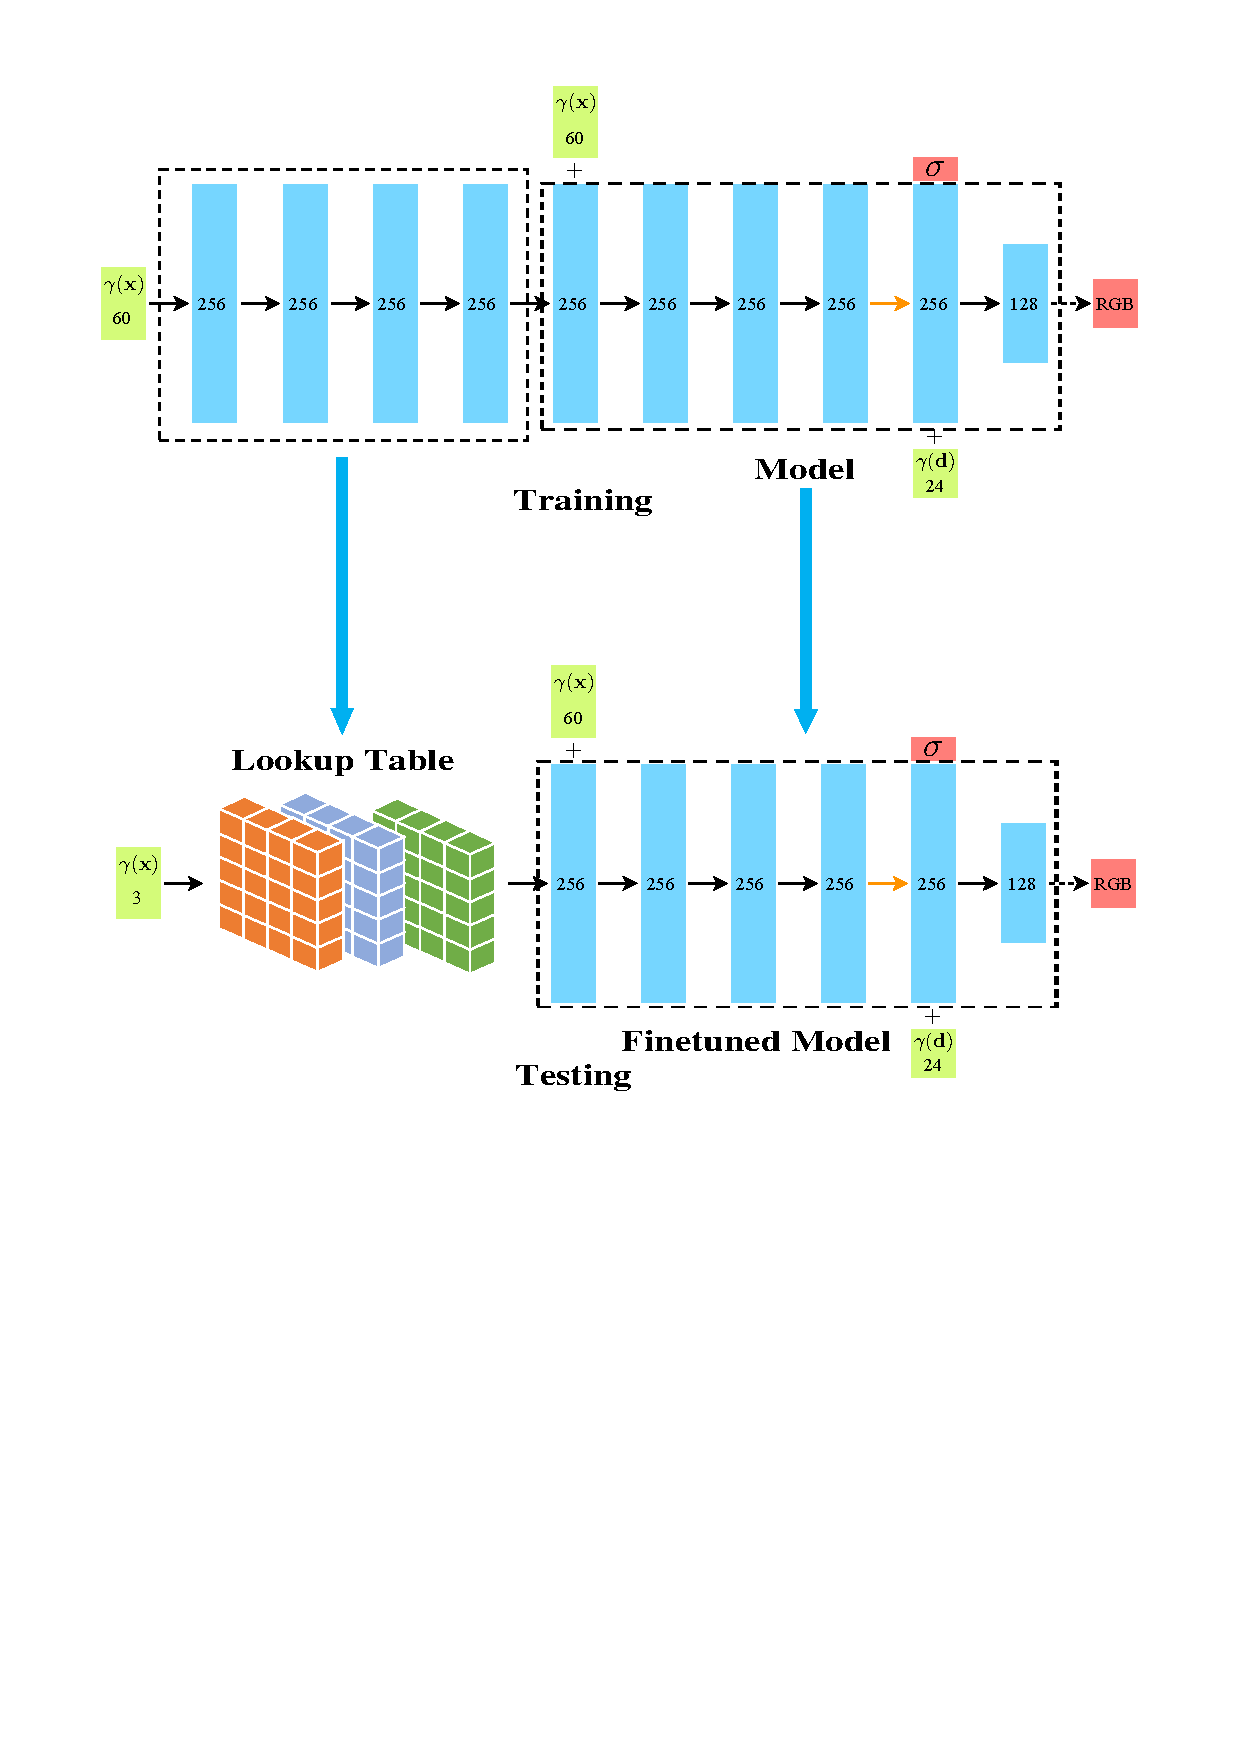
\includegraphics[width=0.95\textwidth]{figures/lookuptable.pdf}
    \caption{查询表的构建以及类似justlookup\cite{lin2019justlookup}的架构,通过缓存网络特征来进行加速,并通过重新训练的方法对近似的特征进行学习。}
    \label{fig:lookuptable}
\end{figure}

本节将详细介绍前一节中查询表的构建,主要介绍查询表的数据类型,获得方式,索引方法,以及如何压缩 NeRF 的网络。

如图~\ref{fig:lookuptable}所示,本文主要的构建方法是首先给采样点训练一个逐点网络,即使用 NeRF 的原网络进行预训练,将网络的前四层全连接层提取出来,我们可以得到一个逐点函数$\mathcal{G}$,类似justlookup\cite{lin2019justlookup},我们使用查询表技术并利用数组索引的方法能够快速地获得近似的函数$\hat{\mathcal{G}}$。

详细地,由前面的理论可知,我们可以用相机光线$\symbf{r}\left(t\right) = \symbf{o} + t \symbf{d}, t \in \left[t_n, t_f\right]$表示一组采样点的集合,为了使用方便,事先对光线的坐标范围进行尺度缩放,使的
$\forall t \in  \left[t_n, t_f\right], \symbf{r}\left(t\right) \in \left[-1, 1\right]^3$。

先忽略位置编码函数$\gamma\left(\cdot\right)$的影响,假设逐点网络输入的是三维坐标点,那么我们可以将上述的映射$\mathcal{G}$表示为$\mathcal{G}: \mathbb{R}^3 \Rightarrow \mathbb{R}^l$, 其中$l$在是第四层全连接网络输出变量的个数,在本文中$l = 256$。更具体地,$\mathcal{G}$是由四层 MLP 实现的,每一层的输出的数目分别是256,256,256,256。

为了学习$\mathcal{G}$,我们利用原网络剩下的部分记为 Model 。使用公式~\ref{eq:nerf_loss}中的均方误差联合优化这个端到端的网络,最终得到三元函数$\mathcal{G}$。一旦我们获得了$\mathcal{G}$,我们就可以通过构建一个查询表来获得近似的函数$\hat{\mathcal{G}}$。

显然,我们现在的最重要的一步是为$\mathcal{G}$构建查询表。为了方便,我们还是假设输入被缩放到一个固定大小的立方体$\mathcal{V}$里,其中$\mathcal{V} = \left[-1, 1\right]^3$。接着将$\mathcal{V}$分成规则的$M^3$个相等的体素块。那么每一个体素的边长则为$\Delta = \frac{2}{M}$。
% 那么因此立方体$\mathcal{V}$则被分成了:
% \begin{equation}
%     \mathcal{V} = \bigcup_{i,j,k}\left[i\Delta, \left(i + 1\right)\Delta\right] \times \left[j\Delta, \left(j + 1\right)\Delta\right] \times \left[k\Delta, \left(k + 1\right)\Delta\right], \mbox{其中} \left(i, j, k\right) \in \left[0, M\right]^3.
% \end{equation}

区别于justlookup\cite{lin2019justlookup},我们并没有采取$T\left[i\right]\left[j\right]\left[k\right] = \mathcal{G}\left(i\Delta, j\Delta, k\Delta\right), \left(i, j, k\right) \in \left[0, M\right]^3$,即存下所有格点所对应的特征,这样在 NeRF 这样细粒度的渲染工作中几乎是不可取的。实际中,我们需要使用 float32 的数据类型去存储,那么总内存开销就会达到$32M^{3}l bits$,以$l = 256, M = 256$为例,则需要$\SI{16}{GB}$的内存,随着查询表的边长$M$增加,内存是以三次方的速度在增长,这在实际操作中是不可行的。

\begin{figure}[b]
    \centering
    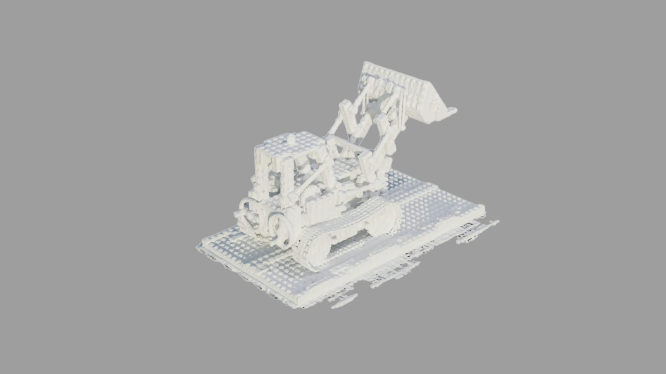
\includegraphics[width=0.95\textwidth]{figures/legomesh_gray_complete.png}
    \caption{使用 NeRF 网络(体密度 $> 0$)提取出的乐高的网格结构}
    \label{fig:lego_mesh}
\end{figure}

为此,我们必须采取相应的措施去压缩查询表。受 DeepSDF \cite{park2019deepsdf}的启发,在 DeepSDF 这篇工作中,可以通过输出的 SDF 值,利用 marching cubes 算法\cite{lorensen1987marching}重建物体的几何结构,类似地,我们知道 SDF 的物理含义是某一三维坐标点到物体表面的最短距离,负值表示在物体内部,正值表示在物体外部,零值则是物体表面;那么,NeRF 输出的体密度信息也有着相似的性质,体密度的物理含义是相机光线终止于某一点的概率,那么同样地,体密度为零值也可以表征物体的表面, 图~\ref{fig:lego_mesh}就是用 NeRF 模型提出乐高玩具的 mesh 结构。根据公式~\ref{eq:weight}可以看出当体密度为负值时权重$w_i$是负值是没有意义的,这也与 NeRF 的处理方式相同,NeRF 在体密度输出的时候使用了 ReLU 函数,因此我们可以认为负值的体密度对渲染的贡献可以忽略。那么结合上一节,如果我们可以将采样点约束在物体表面附近,那么将能获得更好的渲染效果,这可以补偿减少一个网络带来的质量下降的问题。

基于以上的分析,我们假设正值的体密度表征物体的内部,接下来就可以对原查询表进行压缩。我们的目标是只存$\mathcal{V}$中输出的体密度大于零的格点,这样可以大大减少内存的开销。

具体地,我们记从三维坐标点到输出体密度这一部分网络对应的函数为$\mathcal{Q}$,此时压缩后的查询表为:
\begin{equation}
    T_{shrinked} = \left\{
    \mathcal{G}\left(i\Delta, j\Delta, k\Delta\right) | \mathcal{Q}\left(i\Delta, j\Delta, k\Delta \right)  > 0, \left(i, j, k\right) \in \left[0, M\right]^3 
    \right\}.
\end{equation}
至此,我们获得了最终的查询表,由于此查询表是不规则的,或者可以认为是稀疏矩阵,因此索引此查询表也跟常规的方法不同,接下来将详细介绍经过压缩后的查询表的索引。

对于$ T_{shrinked}$ 的存的每一个格点$\left(i\Delta, j\Delta, j\Delta\right)$, 我们必须将每一个常规索引$\left(i, j, k\right)$ encode 到一个唯一值 code ,换句话说,我们的目标是使的$\mathcal{V}$中的任何一个格点对应的code都是不重样的。为此,我们可以使用以下的函数:
\begin{equation}
    \mathcal{E}\left(i, j, k\right) = i + j\cdot M + k\cdot M * M, \left(i, j, k\right) \in \left[0, M\right]^3,
\end{equation}

这个对索引的编码操作可以使得将$\mathcal{V}$中的所有格点都区分开。

接下来,我们将建立一个 code 到 $T_{shrinked}$的查询表$\mathcal{H}$,。具体的建立方式为,
\begin{enumerate}
    \item[a)] 首先建一个大小$size = M + M^2 + M^3$的查询表$\mathcal{H}$,使之能装下$\mathcal{V}$中所有格点;
    \item[b)] 按照$T_{shrinked}$对应的所有点的顺序,假设其中一个点对应的常规索引为$\left(i, j, k\right)$,该点在$T_{shrinked}$的位置为$index$对其使用 encode 操作得到$code = \mathcal{E}\left(i, j, k\right)$;
    \item[c)] 之后填充查询表$\mathcal{H}$,具体做法是$\mathcal{H}[code] = index$。
\end{enumerate}
严谨来说,非$T_{shrinked}$的点在索引时,其$code$ 可能会超过$T_{shrinked}$的索引范围,因此,我们必须处理此问题。具体做法是,在$T_{shrinked}$的最后面加一个哨兵,即增加一个$l$维的全零的向量,假设目前$T_{shrinked}$存了$S$个点对应的特征。而$\mathcal{H}$在初始化的时候,初始值都设置为$S-1$,即当$\left(i, j, k\right)$不在查询范围内时,其$code$可以通过$\mathcal{H}$映射到$S-1$,那么将获取$T_{shrinked}\left[S-1\right]$的值,从而得到一个鲁棒的索引过程。

至此,我们可以总结整个索引的过程。给定一个空间直角坐标系的三维坐标点$\left(x, y, z\right)$,首先通过下面式子计算其常规索引:
\begin{equation}
    \left(i, j, k\right) = \left(\left \lfloor \frac{x + 1}{\Delta} \right \rfloor, \left \lfloor \frac{y + 1}{\Delta} \right \rfloor, \left \lfloor \frac{z + 1}{\Delta} \right \rfloor\right),
\end{equation}

有了常规索引后,需要对其进行 encode ,得到 $code = \mathcal{E}\left(i, j, k\right)$,之后通过 $\mathcal{H}$ 查询到 $code$ 对应的在$T_{shrinked}$中的索引,则整个查询过程为:
\begin{equation}
    T\left[i \right]\left[j \right]\left[k \right] = T_{shrinked} \left[\mathcal{H}\left[\mathcal{E}\left(i, j, k\right) \right] \right].
\end{equation}

最终,如果我们提前缓存了$T$,则可以使用$T\left[i \right]\left[j \right]\left[k \right]$的值去估计$\hat{\mathcal{G}}\left(x, y, z\right)$,因此$\hat{\mathcal{G}}$的将是非常快的,它的开销只取决于访问内存的时间。

显然,我们直接将$\hat{\mathcal{G}}$馈入到经过训练的模型 $Model$中会使渲染效果下降的,因为$\hat{\mathcal{G}}$并不完全正确
等于$\mathcal{G}$,$\hat{\mathcal{G}}$仅仅是$\mathcal{G}$的一个近似。因此为了保持渲染质量不下降,我们在构建了查询表$T$后,需要基于$\hat{\mathcal{G}}$对$Model$进行再学习(或着叫微调),这一操作能显著提升渲染质量,在$M = 200$的时候甚至可以达到和原始 NeRF 质量相当的性能。图~\ref{fig:lookuptable}表征了$\mathcal{G}$是如何由我们的方法实现的。

\subsection{查询表与本文方法的结合}
我们在上一小节详尽地叙述了查询表的创建过程,包含是如何用查询表的构建,索引,压缩,还有通过近似$\mathcal{G}$来进行加速,通过再学习将损失的质量调回原 NeRF 水平。接下来,本节将详细介绍查询表的第二重加速功能:将查询表应用于 NeRF 的采样过程。

如果只是使用查询表去近似$\mathcal{G}$,那么这并没有完全展现出本文最核心的方法。实际上,在上一小节中,我们不止做了这么多工作。我们都知道,在查询表的构建过程中,本文是对查询表进行了压缩的操作,这表面上只是为了减少查询表内存开销,事实上我们还应用了 NeRF 体密度的特性。

由于我们是使用的体密度$\sigma > 0$这一阈值条件对$\mathcal{V}$中格点进行筛选,仅在$T_{shrinked}$中保留其体密度为正值的点所对应的特征(即$l$维向量),并且我们还在$T_{shrinked}$的最后放置了哨兵来表征没有查询到相应点的特征。

因此,我们可以合理地使用$\mathcal{H}$和$T_{shrinked}$这两个查询表对输入的点进行判断,显然如果可查询到,则该点在物体内部,否则不在物体内部。具体地,由于设置了哨兵,我们实际可以只使用索引转换查询表$\mathcal{H}$。对于任意的常规索引$\left(i, j, k\right) \in \left[-1, 1\right]^3$,计算$\mathcal{H}\left[\mathcal{E}\left(i, j, k\right)\right]$的查询结果,若结果为$S - 1$,则原世界坐标$\left(x, y, z\right)$则不在物体(场景)的内部,若结果不为$S - 1$,则在物体内部。

\begin{figure}[t]
    \centering
    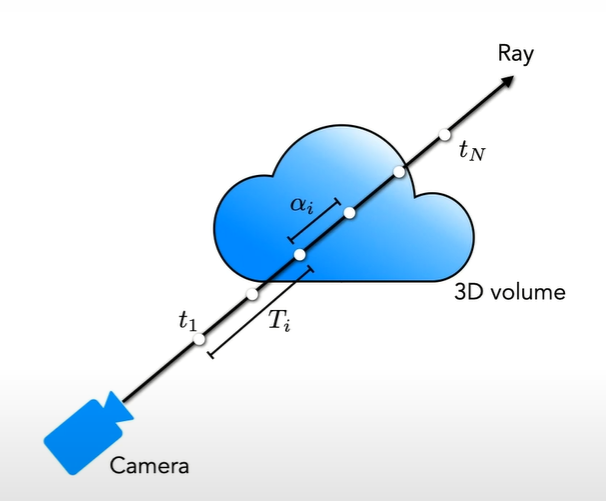
\includegraphics[width=0.95\textwidth]{figures/cloud.jpg}
    \caption{体绘制的采样示意图}
    \label{fig:cloud}
\end{figure}

有了以上的理论基础,接下来将详尽阐述是如何利用查询表进行采样优化以及加速的。

针对前面两节的概述,我们知道,NeRF 是采用分层抽样的方法,即同时优化 coarse 网络和 fine 网络,通过 coarse 网络的输出去估计公式~\ref{eq:weight}中的权重$\displaystyle w_i$的分布(概率密度函数),这是通过增加网络来提高渲染质量的方法。但同时也很显然,使用两个网络,那么时间开销会增加一倍。

为了加速 NeRF ,我们的目标是去掉一个网络,仅使用一个网络来进行优化和渲染,但是这势必会使的渲染质量下降。考虑到 NeRF 使用两个网络是为了优化采样点的选择,这一点启发了我们,如果使用上述的查询表将采样点约束到物体表面附近,那么渲染质量会比仅使用一个网络显著提升,通过实验证明本文的方法可以在几乎不损失渲染质量的情况下对 NeRF 的推理过程进行加速。下面是查询表是如何和本文方法进行融合的。

如图~\ref{fig:cloud}所示的是体绘制的采样示意图。假设相机光线为$\symbf{r}\left(t\right) = \symbf{o} + t \symbf{d}$,并在$\left[t_n, t_f\right]$的范围内均匀采样$N$个点,深度记为$t_{1}, t_{2}, \cdots, t_{N}$,这些深度是递增的,对应的点的世界坐标为$\symbf{r}\left(t_{1}\right), \symbf{r}\left(t_{2}\right), \cdots, \symbf{r}\left(t_{N}\right)$。分别计算这些点的常规索引,以及编码之后的 code,通过这些 code 去查询$\mathcal{H}$,得到一个长度为$N$的向量$vector$。之后按顺序对$vector$的每一个坐标值进行判断,若值均为$S - 1$,则说明该光线与物体没有交点,则采样点不需要优化,若存在值不为$S - 1$的,则说明光线和物体有交点,记第一个交点对应的深度值为$t_{mid}, mid \in \left\{1, 2, \cdots, N\right\}$。在有交点的情况下,我们需要重新设定采样区间长度为$L$,则新的采样区间为$\left[t_{mid} - L / 2, t_{mid} + L / 2\right]$,此区间能表征物体的表面附近,我们需要在此区间内重新均匀采样$N$个点,${t\prime}_{1}, {t\prime}_{2}, \cdots, {t\prime}_{N}$,然后就可以将$\symbf{r}\left(t\prime_{1}\right), \symbf{r}\left(t\prime_{2}\right), \cdots, \symbf{r}\left(t\prime_{N}\right)$这些采样点送入网络进行训练,最终实验证明使用了改进的采样方式,在我们减少一个网络的时候,可以保证渲染质量几乎不下降。

最终,我们通过缓存一个查询表,成功地在不损失精度的情况下减少了一个网络的开销,对渲染过程进行了加速,那么因此,本文方法对应的 loss 函数变为:
\begin{equation}
    \mathcal{L} = \sum_{\symbf{r}\in \mathcal{R}}\left[\left\|\hat{C}\left(\symbf{r}\right) - C\left(\symbf{r}\right)\right\|_{2}^{2} \right].
    \label{eq:nerf_loss}
\end{equation}

\section{本章小结}
本章首先介绍了本文所研究的问题定义。接着介绍了新视图合成任务中的神经辐射场表示方法,然后在此基础上详细地介绍了本文基于问题而提出的方法论,包含模型网络结构,查询表技术的引入与查询表的构建,以及如何把查询表应用到本文的方法中。

综上,本文借助查询表技术替换了一部分网络(逐点网络)参数,使得查询可以直接从内存(或缓存)中获取中间层的特征,这可以显著加速渲染过程;为了减少查询表的内存开销,同时也是为了与本文方法进行融合,我们对查询表进行了压缩的操作,具体是使用体密度$\sigma > 0$这一阈值条件去筛选位于物体内部的格点;本文的核心方法是减少 NeRF 的原始的两个网络的结构,我们仅采用一个网络进行训练和渲染,为了保证质量不下降,使用查询表判断原始采样点并第一个在物体内的点,并在此附近进行重新的均匀采样,可以补偿只用一个网络带来的质量下降;当然,最关键的一点是,将上述方法结合在一起时,由于查询表替换网络这一部分是用的近似特征,因此为了保证质量不下降,必须进行近似特征再学习。最终,通过本文的方法可以实现在几乎不损失精度的情形下对 NeRF 合成新视图进行加速。

\cleardoublepage

\cleardoublepage
% !TeX root = ../main.tex

\chapter{实验部分}\label{equations}
为了验证本文提出的加速 NeRF 的方法的有效性,本章将详尽地描述所做的相关的验证性和解释性实验,首先将本文提出的方法命名为 F-NeRF。首先将介绍实验的基本设置,包含使用的深度学习框架、开发语言、训练集和测试集,其次给出 F-NeRF 在合成新视图这样任务上的基本效果,然后详尽地描述 F-NeRF 的预训练过程,训练过程,相关参数配置,接着描述 F-NeRF 在合成数据集 Synthetic-NeRF 和真实场景数据集 LLFF-NeRF 上的实验效果以及分析。最后根据实验效果给出实验结论并进行总结。
\section{实验基本设置}\label{experiment-set}
首先先介绍下本文实验的基本设置,包含开发环境和实验所需的数据集。
\subsection{开发环境}
现如今的深度学习框架有很多,包含Caffe、Tensorflow和Pytorch等。Caffe是基于 C++ 语言开发出的深度学习框架,当然也提供 python 的接口,核心是使用 C++ 开发的,也因此更高效,适合工业界开发,但它缺少灵活性和拓展性,环境配置复杂。Tensorflow 是目前应用最广泛的深度学习框架,由谷歌公司开发与维护,具有十分成熟的社区与工具,已经广泛地被应用到企业中了。Pytorch 是相对较新的深度学习框架,由 Facebook 开发与维护的,以代码简洁上手容易,容易实现并行等优点进入到开发者的视野中,现在越来越受到学术界和工业界的青睐。由于查询表使用 Pytorch 实现更为简便,所以本文使用 Pytorch 来实现神经辐射场的所有结构。使用其他框架也可以完全复现本文的方法。本文基于 Ubuntu 18.04操作系统进行开发,开发语言为 python 3.6。使用的 GPU 是一张显存为12GB的 NVIDIA Titan X。 
\subsection{数据集} \label{Dataset}
在整个新视图合成的实验中,本文使用的都是广泛使用的公开的数据集,包含合成数据集 Synthetic-NeRF 和真实世界数据集 LLFF-NeRF。下面将大致介绍下这两种数据集。
\begin{enumerate}
    \item[1)] Synthetic-NeRF 数据集:这个合成数据集是 NeRF 生成并使用的,包含由 blender 渲染的八个物体,每一张图都是$800 \times 800$的分辨率。本文为了加速训练的过程,实验中实际使用的是下采样到$400 \times 400$分辨率的图像。对于每一个物体,有100个视角作为训练集,200个新视角作为测试集。Synthetic 数据集的优点是,它拥有绝对准的相机位姿,这能够排除受位姿影响而带来的质量的下降。如图~\ref{fig:Chairs} 是该数据集的示意图。
    \item[2)] LLFF-NeRF 数据集:这个真实数据集包含八个前向场景的图像,其中五个来自于 LLFF\cite{mildenhall2019local},三个来自于 NeRF。每个场景包含20到62张图,其中$1/8$用作测试。所有的图像都有着$1008 \times 756$的高分辨率。本文为了加速训练的过程,实验中实际使用的是下采样到$504 \times 378$分辨率的图像。如图~\ref{fig:T-Rex} 是该数据集的示意图。
\end{enumerate}

\begin{figure}[thbp]
    \centering
    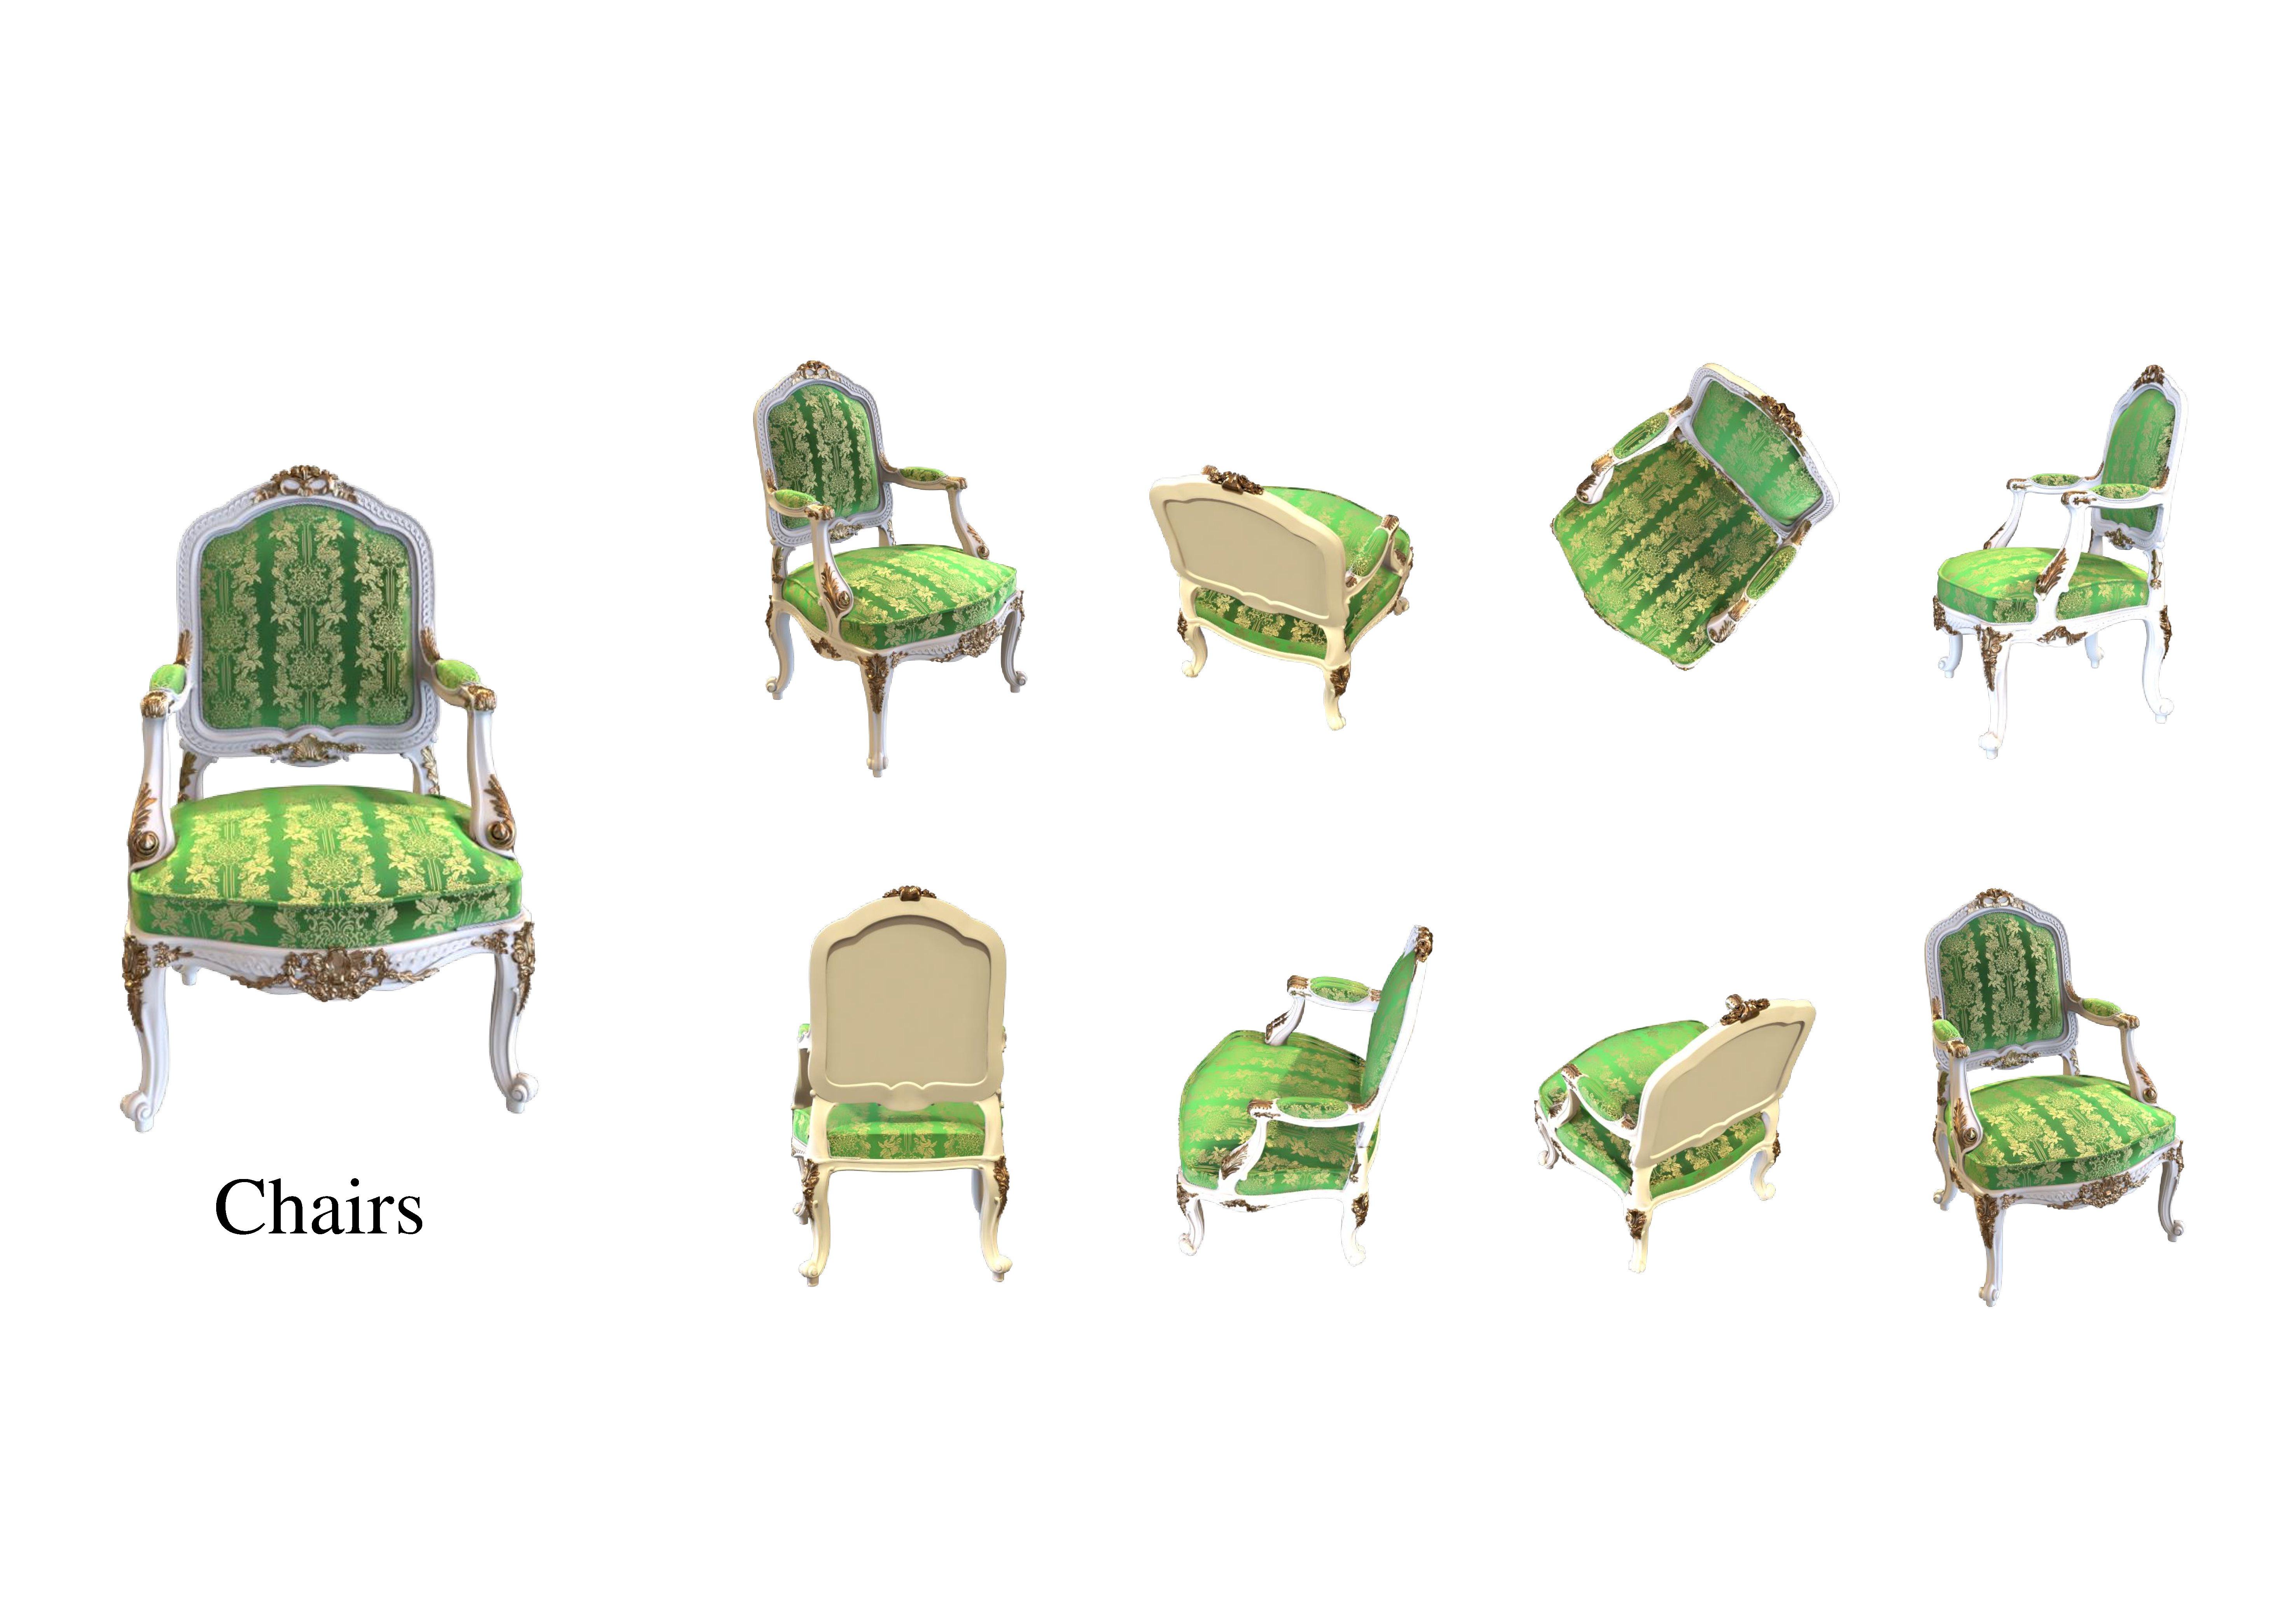
\includegraphics[width=0.95\textwidth]{figures/Chairs.pdf}
    \caption{Synthetic-NeRF 数据集示意图,第一行是部分训练集,第二行是部分测试集}
    \label{fig:Chairs}
\end{figure}

\begin{figure}[thbp]
    \centering
    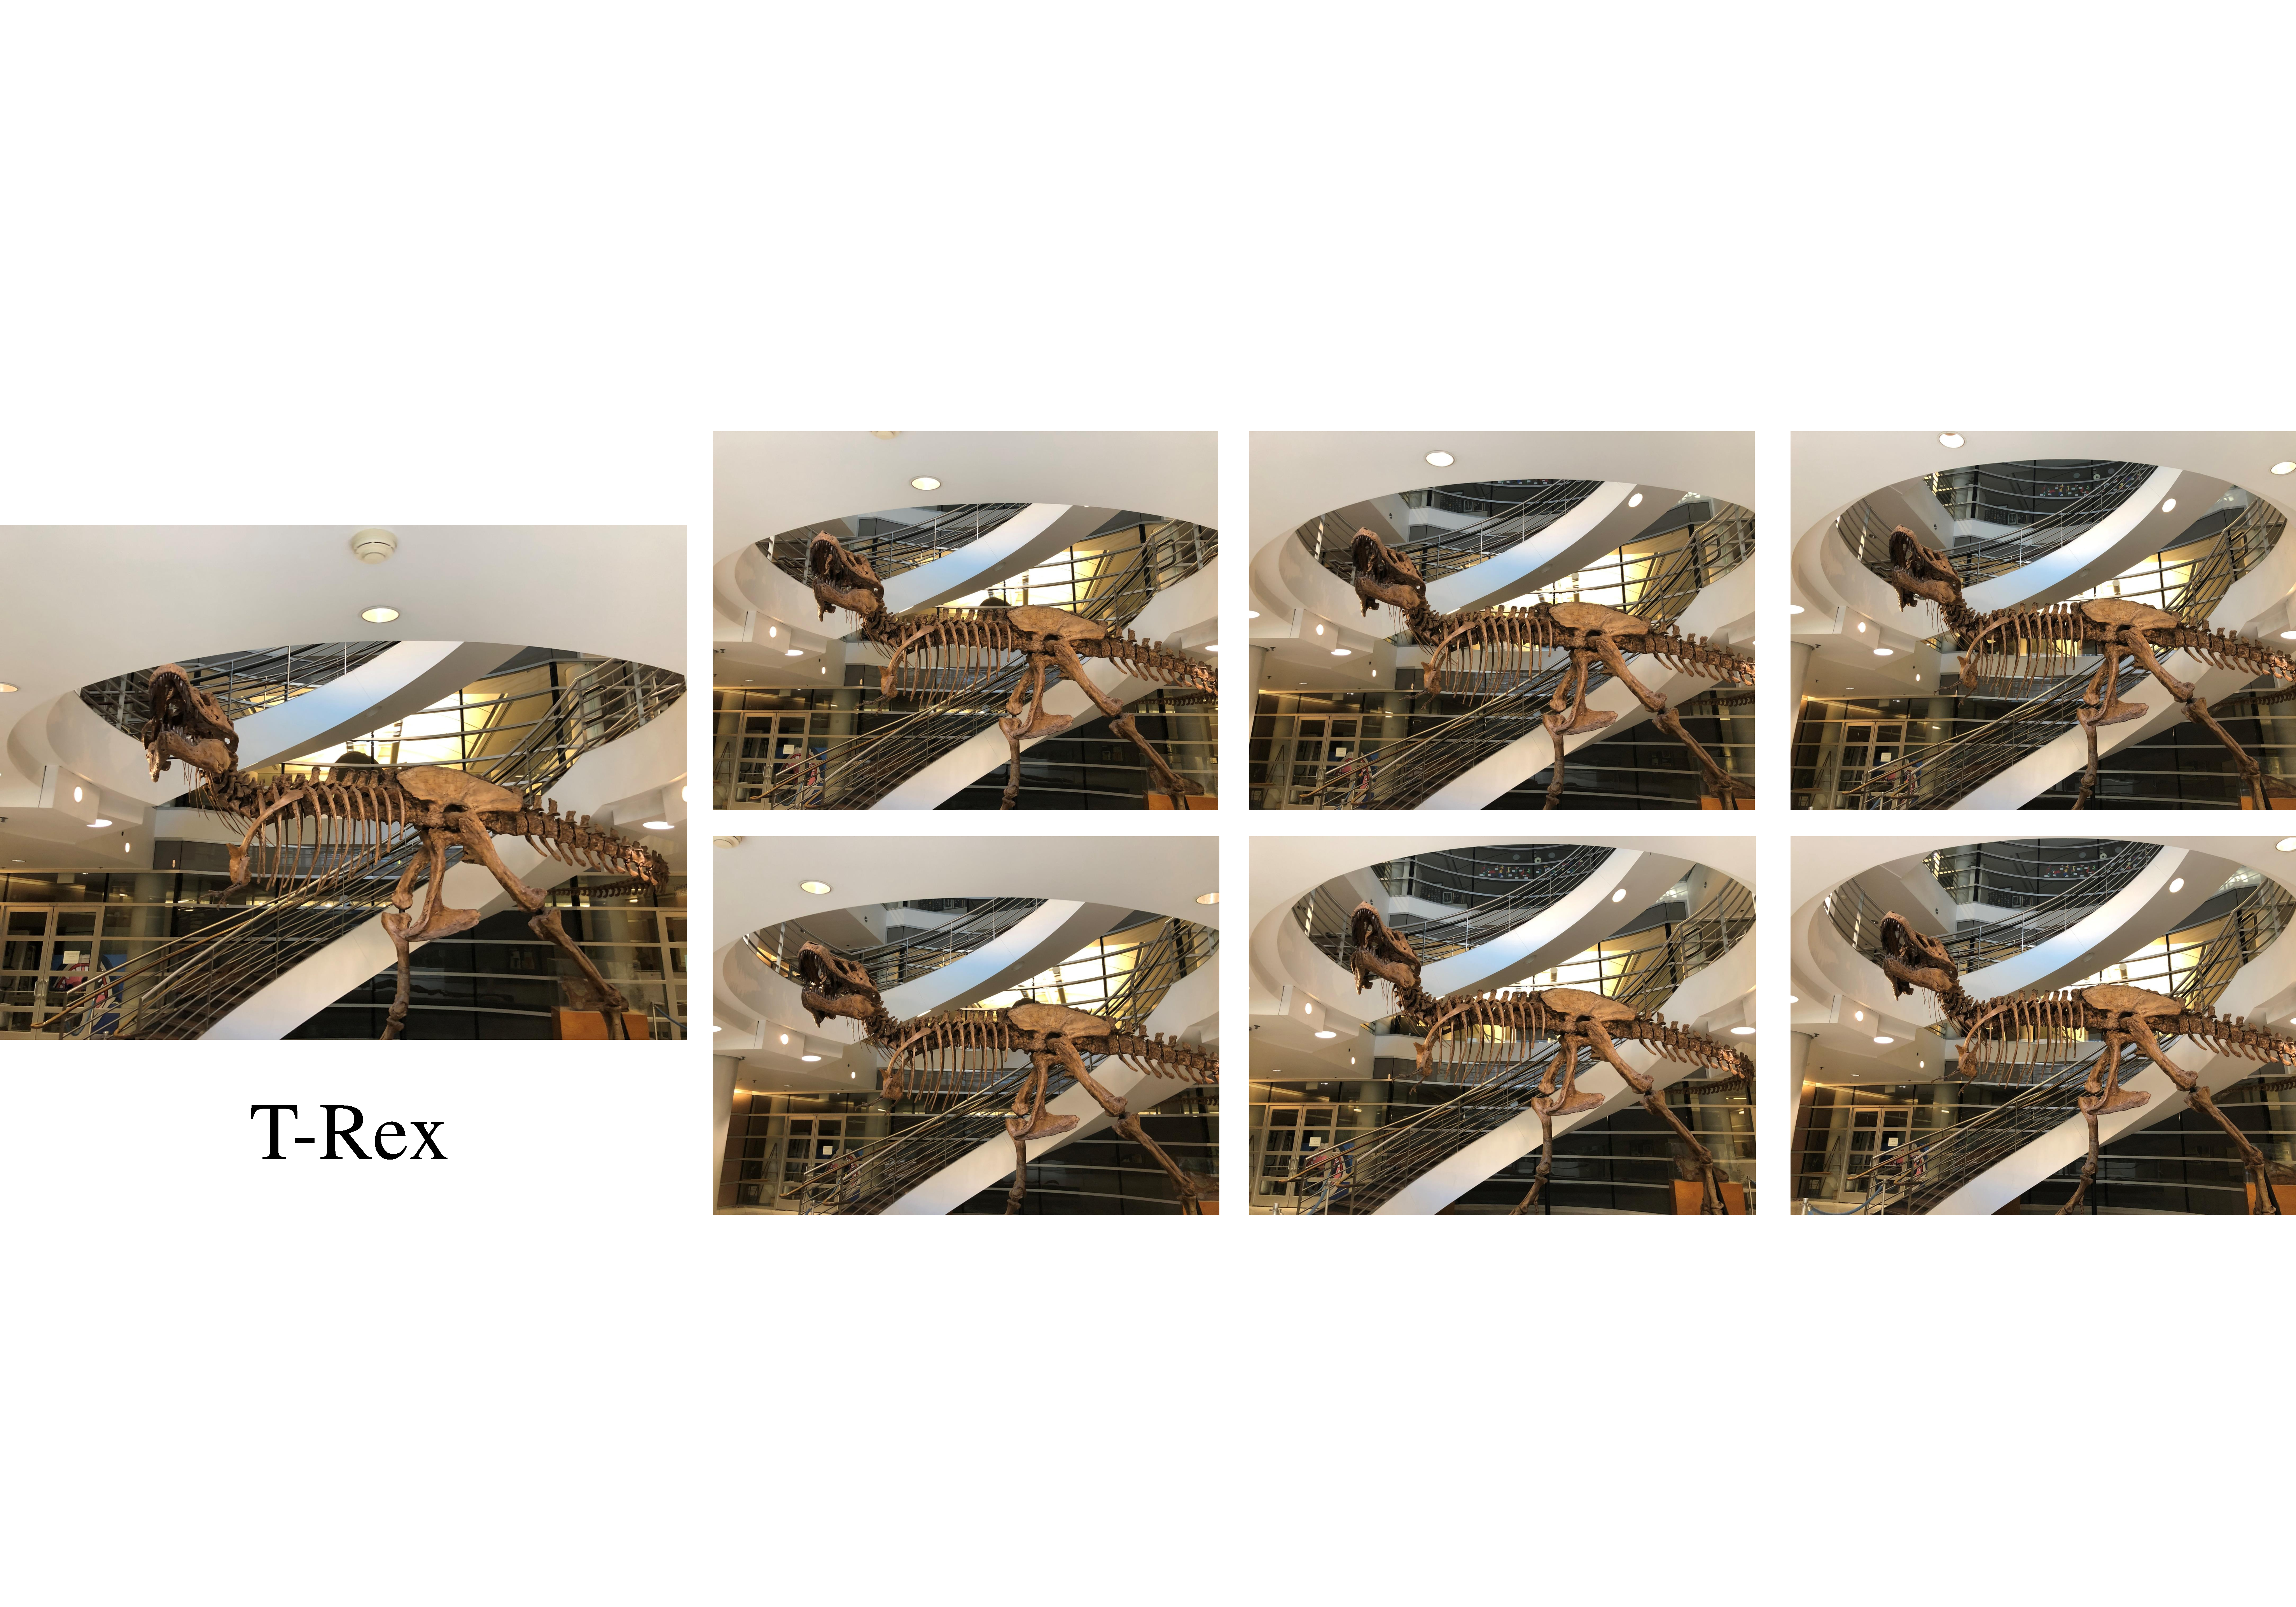
\includegraphics[width=0.95\textwidth]{figures/T-Rex.pdf}
    \caption{LLFF-NeRF 数据集示意图,第一行是部分训练集,第二行是部分测试集}
    \label{fig:T-Rex}
\end{figure}
\newpage

\section{实现细节}\label{details}
本文提出的F-NeRF架构具体见~\ref{method} 节。本文的加速模块是缓存了一张查询表,查询表的位置信息反映了物体的近似几何结构,具体缓存的是第四层全连接层输出的特征。

为了得到缓存所需的查询表,首先需要基于 NeRF 网络进行预训练,具体参数为,每个 batch 使用1024条光线,相应地,每条光线上的采样点数目为$N_c = 64$(coarse 网络),$N_f = 128$ (fine 网络)。同样地,使用 Adam 优化器\cite{kingma2014adam},在学习的过程中,学习率从$5 \times 10^{-4}$指数衰减到$5 \times 10^{-5}$(其他的 Adam 超参数使用的是默认值,$\beta_{1} = 0.9$,$\beta_{2} = 0.999$,$\epsilon = 10^{-7}$)。在合成数据集上,对每个物体的训练过程在本文的设备上大概要训练100000 epoch(大约12小时)。真实数据集上,对每个场景的训练大概200000到300000 epoch 会收敛(1到2天)。

得到了预训练的 NeRF 模型后,接下来就可以训练本文的模型 F-NeRF。首先要通过 NeRF 网络缓存一张特征查询表$T$,这个过程大概需要半分钟。为了保证质量几乎不下降,由于本文提出的 F-NeRF 模型只使用了一个网络,那么再使用 coarse 网络的64个采样点就不足以从查询表中探测到物体表面,因此,为了权衡速度与质量,F-NeRF 使用了$N = 128$个采样点,这显然仍然少于$N_c + N_f = 192$。在另一个加速的部分,F-NeRF 使用缓存的$T$替换网络的前四层全连接层,这样在测试的过程中就可以直接从缓存中获取特征,这大大减少了时间开销。以上加速模块的引入显然会导致质量的下降,第一点,去掉了一个 coarse 网络,减少了采样点,第二点,使用了缓存的特征查询表的近似特征,因此,为了保证质量不下降,必须对 F-NeRF 网络进行再训练,两个数据集大约训练100000 epoch 网络可以收敛,将近4小时。

在测试时,本文的方法和 NeRF 一样都需要一组相机参数作为输入,作用于输出图像的每个像素发出的光线上。沿着每条相机光线生成的大量采样点按照 NeRF 的理论进行积分。然而 F-NeRF 能够使用缓存的特征查询表对单网络的采样点进行优化。为了提升性能,本文对将第一次的均匀采样点送入到缓存的查询表中进行查询(使用的是最近邻的插值方式),由于查询表表征的是物体的几何结构表面,因此沿着光线找到第一个击中物体表面的点(或缓存命中),以此为中心在适当范围内进行二次均匀采样,之后将新采样点送入网络,第一步加速完成。为了进一步提升效率,F-NeRF 借助了 justlookup \cite{lin2019justlookup}的思想,查询表缓存的是原 NeRF 网络前四层输出的特征,采样点可以直接通过最近邻内插法在查询表内查询相应的特征,而减少了网络的正向传播层数,这大大加快了渲染的速度。本文的未压缩前的查询表对应的分辨率大小为$200^3$,这是实验硬件设备可支持的最大分辨率。$200^3$分辨率的查询表实质上对应着 \SI{7.63}{GB} 的内存开销,但是经过本文方法进行压缩后,平均仅需要 \SI{0.97}{GB},有效地去除空白的自由空间,这极大地节省了内存,同时也使得查询表隐藏着场景的几何信息。

\section{评测指标}\label{metrics}
\subsection{图像质量指标}
为了评估合成的新视图的质量,实质都是计算合成图像与真实观测的图像之间的差异度。假定合成图像为$\symbf{Y}$,真实图像为$\symbf{X}$,图像均为$M \times N$的彩色三通道图像,假设每个像素使用八位来存储,即像素值范围为$\left[0, 255\right]$。本文使用的质量评估指标如下:
\begin{enumerate}
    \item [1)]峰值信噪比 (Peak Signal to Noise Ratio, PSNR) \\ PSNR 是一个信号处理学科上的概念,物理含义是信号可能的最大功率与噪声功率的比值,一般使用对数分贝来表示。对于图像的情形,可以有以下公式:
    \begin{align}\label{psnr}
        \symup{PSNR} &= 10\log_{10}\left(\frac{255^{2}}{\symup{MSE}^{2}}\right), \nonumber\\
        \textit{其中均方误差} \quad \symup{MSE} &= \frac{1}{3MN}\sum_{R,G,B}\sum_{i = 0}^{M - 1}\sum_{j = 0}^{N - 1}\left[\symbf{X}\left(i,j\right) - \symbf{Y}\left(i,j\right)\right]^{2},
    \end{align}
    PSNR 是相对客观的指标,他是逐像素计算的。由公式~\ref{psnr} 可以看出,PSNR 值越大,对应 MSE 越小,那么合成图像和真实图像直接的差异也就越小。所以,PSNR 这一指标在一定程度上可以反映图像质量的好坏,但是它是比较客观的,不太涉及人眼观感,因此 PSNR 值越大,在人眼看来可能不一定好。所以在对比图像质量的时候,仅仅使用 PSNR 是不够的。\\
    \item [2)]结构相似性度量 (Structural Similarity Index Measure, SSIM\cite{wang2004image}) \\
    结构相似性的基本理念是认为图像是高度结构化的,图像之间的相邻像素有着很强的关联性。人类的视觉系统已经习惯了这种很强的结构化信息,因此在衡量图像质量的时候,推荐使用 SSIM 这一度量指标。具体地:
    \begin{equation}
        \symup{SSIM}\left(X, Y \right) = \left[l\left(\symbf{X}, \symbf{Y}\right) \right]^{\alpha} \cdot \left[c\left(\symbf{X}, \symbf{Y}\right) \right]^{\beta} \cdot \left[s\left(\symbf{X}, \symbf{Y}\right) \right]^{\gamma},
    \end{equation}
    其中$l\left(\symbf{X}, \symbf{Y}\right)$,$c\left(\symbf{X}, \symbf{Y}\right)$ 和$s\left(\symbf{X}, \symbf{Y}\right)$定义如下:
    \begin{align}
        l\left(\symbf{X}, \symbf{Y}\right) &= \frac{2\mu_{x}\mu_{y} + C_{1}}{\mu_{x}^{2} + \mu_{y}^{2} + C_{1}}, \\
        c\left(\symbf{X}, \symbf{Y}\right) &= \frac{2\sigma_{x}\sigma_{y} + C_{2}}{\sigma_{x}^{2} + \sigma_{y}^{2} + C_{2}}, \\
        s\left(\symbf{X}, \symbf{Y}\right) &= \frac{\sigma_{xy} + C_{3}}{\sigma_{x}\sigma_{y} + C_{3}},
    \end{align}
    这里的$l\left(\symbf{X}, \symbf{Y}\right)$、$c\left(\symbf{X}, \symbf{Y}\right)$ 和$s\left(\symbf{X}, \symbf{Y}\right)$分别是亮度、对比度、结构。此外,$\mu_{x}, \mu_{y}$是$\symbf{X}$和$\symbf{Y}$的均值,$\sigma_{x},\sigma_{y}$分别是$\symbf{X}$和$\symbf{Y}$的方差,$\sigma_{xy}$是$\symbf{X}, \symbf{Y}$的协方差。$C_{1} = \left(k_{1} \times 255\right)^{2}$,$C_{2} = \left(k_{2} \times 255\right)^{2}$,$C_3 = \frac{C_2}{2}$。其中,$k_1, k_2$一般取0.01和0.03。实验中,$\alpha$,$\beta$和$\gamma$均置为1。SSIM 的值越大,表明合成图像与真实图像结构越相似。\\
    \item [3)]感知相似度(Learned Perceptual Image Patch Similarity, LPIPS\cite{zhang2018unreasonable}) \\
    该指标是基于深度学习的度量方法,这是借助了深度学习能够提取到更细粒度的图像特征,并进行对比,该指标比 PSNR、SSIM 更能符合人类的感知情况。感知损失的计算方式为:
    \begin{equation}
        d\left(\symbf{x}, \symbf{x}_{0}\right) = \sum_{l}\frac{1}{H_{l}W_{l}}\sum_{h, w} \left\| \symbf{w}_{l}\odot \left(\hat{\symbf{y}}_{hw}^{l} - \hat{\symbf{y}}_{0hw}^{l}\right)\right\|_{2}^{2},
    \end{equation}
    这里$\symbf{x}, \symbf{x}_{0}$是输入的图像,$l$是网络的层数,$\hat{\symbf{y}}_{hw}^{l}, \hat{\symbf{y}}_{0hw}^{l}$表示第一层网络的特征图,$\symbf{w}_{l}$为权重。上述也表明了 LPIPS 实际是计算了两张图之间的特征距离,因此值越小表征两张图像越相似。\\
\end{enumerate}

结合上述三个质量指标,分别可以从客观,结构,人类感知多个维度来评价合成图像与原图的差别,其中 PSNR 和 SSIM 是值越大质量越好,而 LPIPS 是值越小合成的图像与原图差异越小,质量越高,这样的质量评价体系更完整、更准确、也更公平。

% 为了评估本文提出的F-NeRF的质量,我们使用峰值信噪比 (Peak Signal to Noise Ratio, PSNR) ,结构相似度 (Structural Similarity, SSIM\cite{wang2004image}),以及具有人类感知的 LPIPS\cite{zhang2018unreasonable} 来将输出与 ground truth 进行对比。PSNR 是逐像素计算,用于测量两个输入图像之间的差异。 SSIM 是基于结构信息退化的感知图像质量评估。 在两个指标(PSNR和SSIM)中,值越大表示性能越好。 LPIPS是基于受过训练的网络的深层功能的最新感知度量,它与人类相似性判断更加一致,而较低的值表示更好的结果。

\subsection{渲染速度指标}
速度指标这里就比较简单,没有质量那么难以评估,因为速度是客观的,不受人的主观意识判断,常规地,可以使用时间或者帧率对速度进行表征。其中,时间是值越小越好,而帧率则相反。在本文后与实验部分,统一使用时间这一度量指标来表征速度,具体使用的单位是 s/frame,即渲染一帧所需的时间。


\begin{figure}[tbhp]
    \centering
    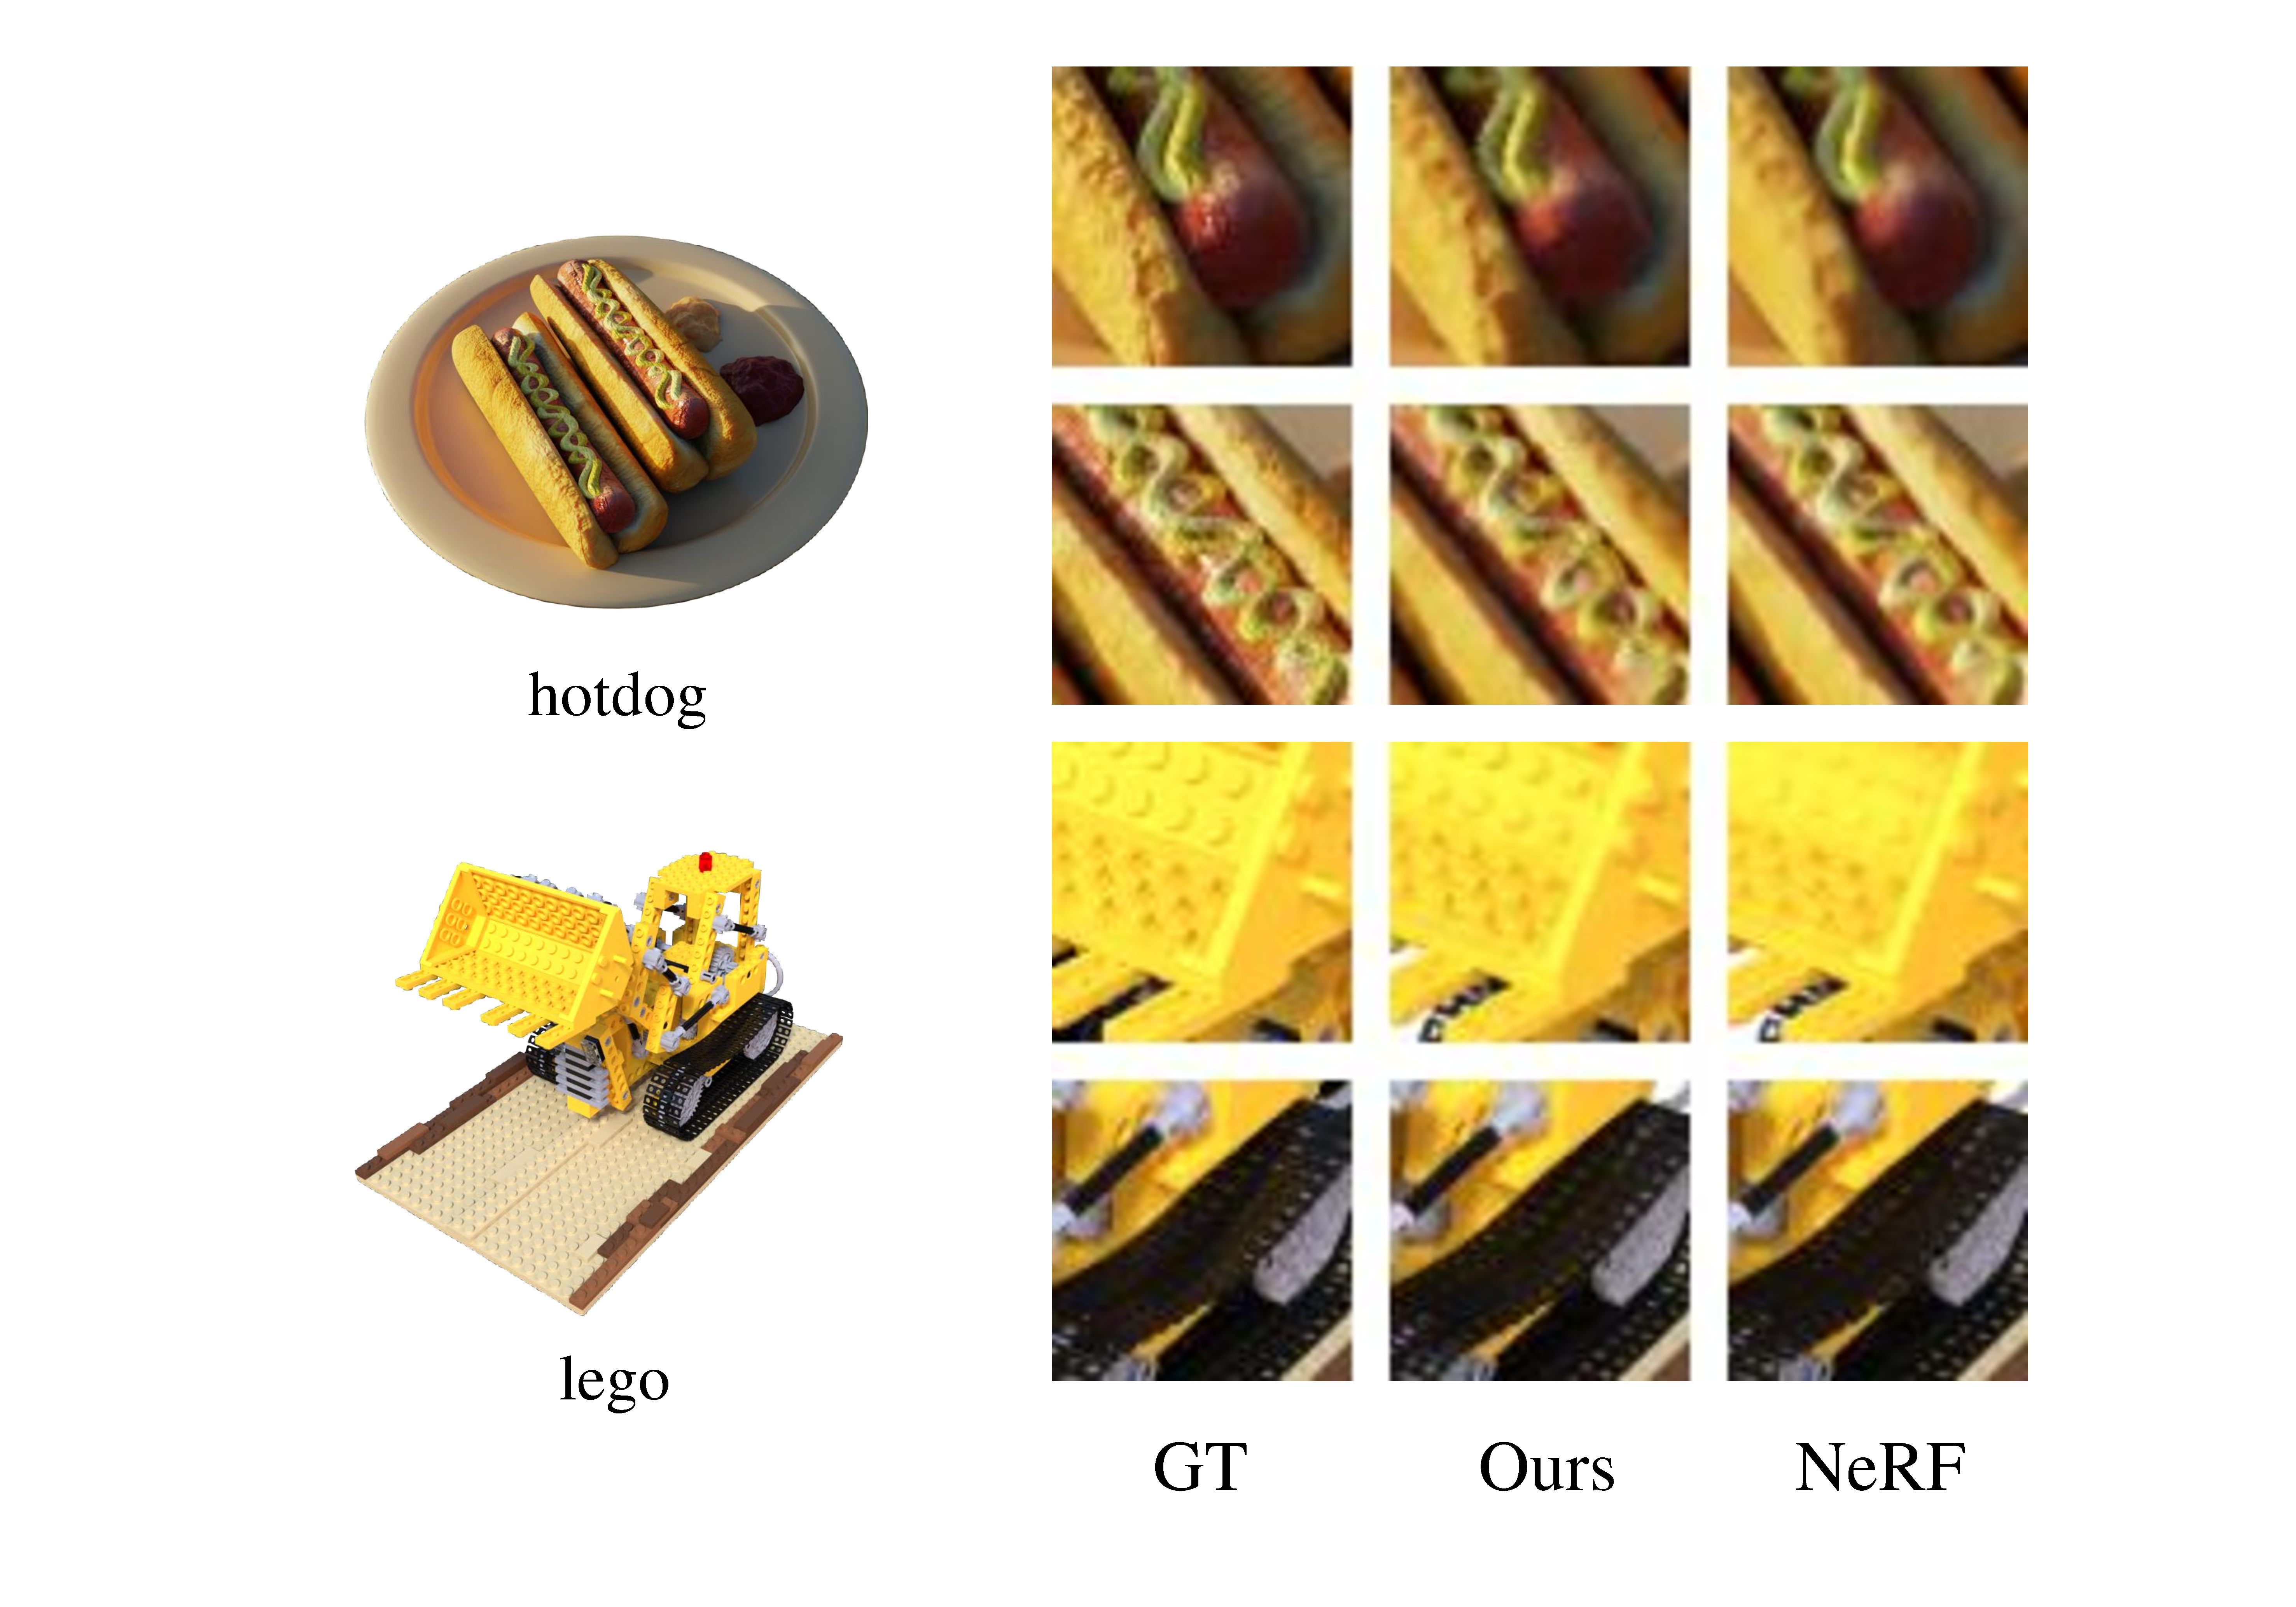
\includegraphics[width=0.95\textwidth]{figures/synthetic.pdf}
    \caption{F-NeRF 与 NeRF 在合成数据集Synthetic-NeRF上的定性比较,使用的是分辨率为$400^2$的图像。}
    \label{fig:synthetic}
\end{figure}

\begin{table}[t]
	\caption{本文提出的 F-NeRF 与 NeRF 在 PSNR,SSIM,LPIPS以及渲染一帧图像的时间上的定量对比,其中 PSNR 的单位是分贝(\si{dB}),时间的单位是秒/帧 (s/frame)}
	\label{tab:synthetic}
	\centering
	{\small\def\arraystretch{1.4}\setlength\tabcolsep{6pt}
		\begin{tabular}{cccccccccc}
			\toprule
					
			& Chair & Drums  & Ficus  & Hotdog &  Lego  & Materials & Mic & Ship & Mean\\
			\hline
			\multicolumn{10}{c}{PSNR $ \uparrow$} \\
			\hline
			NeRF   & 31.21	&\textbf{24.72}	&\textbf{28.19}	&33.03	&31.01	&28.65	&30.08	&\textbf{26.43}	&29.16\\
			\textbf{Ours} & \textbf{32.11}	&24.42	&27.84	&\textbf{35.10}	&\textbf{31.15}	&\textbf{28.79}	&\textbf{31.53}	&26.14	&\textbf{29.64}\\
			\hline
			\multicolumn{10}{c}{SSIM $ \uparrow$} \\
			\hline
			NeRF   &0.966	&\textbf{0.921}	&\textbf{0.962}	&0.958	&0.950	&0.941	&0.972	&\textbf{0.835}	&0.938\\
			\textbf{Ours} & \textbf{0.968}	&0.908	&0.955	&\textbf{0.972}	&\textbf{0.958}	&\textbf{0.951}	&\textbf{0.985}	&0.817	&\textbf{0.939}\\
			\hline
			\multicolumn{10}{c}{LPIPS $ \downarrow$}\\
			\hline
			NeRF   & 0.046	&\textbf{0.091}	&\textbf{0.044}	&0.121	&0.056	&0.063	&0.028	&\textbf{0.173}	&0.077\\
			\textbf{Ours} & \textbf{0.045}	&0.100	&0.058	&\textbf{0.044}	&\textbf{0.051}	&\textbf{0.053}	&\textbf{0.019}	&0.196	&\textbf{0.071}\\
			\hline
			\multicolumn{10}{c}{Time $ \downarrow$}\\
			\hline
			NeRF   & 15.23	&15.25	&14.89	&16.15	&15.68	&15.87	&15.01	&15.29	&15.42\\
			\textbf{Ours} & \textbf{4.71}	&\textbf{4.54}	&\textbf{4.80}	&\textbf{4.94}	&\textbf{4.84}	&\textbf{4.88}	&\textbf{4.67}	&\textbf{4.57}	&\textbf{4.74}\\
			\bottomrule
		\end{tabular}
	}
\end{table}

\newpage

\section{实验结果与分析}\label{results}
下面介绍本文的实验结果与分析部分。本文分别在公开的合成数据集 Synthetic-NeRF 和真实数据集 LLFF-NeRF 上进行了新视图合成任务的实验,上述数据集的具体细节在~\ref{Dataset} 小节。分别在这两个数据集下对实验结果进行分析。
\subsection{基于 Synthetic-NeRF 数据集的实验}
为了验证本文提出的加速方法的有效性,首先本文在公开的合成数据集 Synthetic-NeRF 的八个物体上进行了实验验证。合成数据集的场景相对简单,位姿是绝对准确的,这对于评估质量来说很有帮助。图~\ref{fig:synthetic} 给出了本文提出的 F-NeRF 与 NeRF 的定性对比结果。从结果可以看出,F-NeRF 几乎达到了和 NeRF 一样的质量,甚至在一些细节上,本文提出的 F-NeRF 还做的比较好,比如 hotdog 的沙拉酱部分,还有 lego 的铲斗部分,这一定程度上反映了本文提出的方法能够获取比较靠近表面的采样点,因为这些采样点对渲染过程的贡献更大。

表~\ref{tab:synthetic} 提供了 F-NeRF 与 NeRF 在合成数据集下的具体定量指标对比。从表格中可以看出,本文提出的方法 F-NeRF 在几乎不损失精度的情况下能够在渲染速度上为 NeRF 加速3.2倍。质量方面,F-NeRF 在 PSNR 和 SSIM 这两项指标的均值略高于 NeRF,在 LPIPS 这一指标上比 NeRF 低0.006。F-NeRF 仅在 Drums、Ficus、Ship这三个物体上的质量略低于 NeRF,这可能是因为这些物体的空洞较多,而原 NeRF 网络预测的体密度不是绝对准确的,可能会把物体内部或表面预测为物体外部而没有存在查询表中,那么该查询表就会丢失许多信息,难以把采样点的位置都约束在物体表面附近。不过,从整体上看,本文提出的 F-NeRF 几乎是达到了 NeRF 的质量水平。

以上结果表明,本文提出的新视图合成加速方法在合成数据集上能够为 NeRF 实现几乎无质量损失的显著加速。

\pagebreak
\begin{table}[htbp]
	\caption{真实世界数据集下的质量与渲染速度对比(八个场景的均值)}%
	\centering
	{\small\def\arraystretch{1.4}\setlength\tabcolsep{12pt}
			
		\begin{tabular}{lcccc}
			%\hline
			\toprule
			&PSNR (dB) \uparrow & SSIM\uparrow & LPIPS\downarrow & Speed (s/frame) \downarrow\\
			\midrule
			SRN\cite{sitzmann2019scene}         & 22.84  & 0.668  & 0.378 & -\\
			LLFF\cite{mildenhall2019local}   		 & 24.13  & 0.798  & \textbf{0.212} & -\\
			NeRF\cite{mildenhall2020nerf}   		 & 26.50  & 0.811  & 0.250 & 14.33\\
			\textbf{Ours} & \textbf{26.87}  & \textbf{0.836}  & 0.226 &\textbf{4.23}\\
			\bottomrule
		\end{tabular}
	}
		%
	\label{tab:real}
\end{table}

\subsection{基于 LLFF-NeRF 数据集的实验}
真实场景相对于合成场景更为复杂,受光照条件、相机标定等因素的影响,因此合成高质量的新视角下的图像是相对困难的。本小节将本文提出的 F-NeRF 方法应用在 LLFF-NeRF 数据集上,与目前最先进的方法 SRN\cite{sitzmann2019scene} ,LLFF\cite{mildenhall2019local},以及 NeRF\cite{mildenhall2020nerf}进行对比。真实场景的相机位姿都是通过 COLMAP \cite{schonberger2016structure} 方法计算的。

图~\ref{fig:llff} 给出了本文与 NeRF 在真实场景下的定性对比图,本文将图像中相对细节较多较复杂的部分使用红蓝框给框起来,读者可以自行放大进行对比。从图中可以看出,本文的方法在渲染的新视图的质量方面达到了几乎和 NeRF 相同的水平。具体地,对于图中的 T-Rex 场景,对应于红色框的部分,可以看出,本文的 F-NeRF 和 NeRF 都出现了细节的严重丢失,这是因为该物体过于细小,比较难采样到稳定的采样点,但事实上,F-NeRF 丢失的细节较 NeRF 还是要少一些,这是因为 F-NeRF 在采样上进行了优化,利用查询表缓存相关的几何信息,使得采样到的点是位于物体表面的对渲染贡献较高的部分。

最后表~\ref{tab:real} 给出了本文与其他方法的定量指标的对比(取八个场景的均值),可以看出本文提出的 F-NeRF 在 PSNR 上平均比 NeRF 提高\SI{0.37}{dB},在 SSIM 上能提升0.033,在 LPIPS 上能降低0.024,此外更能够给 NeRF 在渲染速度上加速3.4倍,这将使得基于神经辐射场的新视图合成系统的构建提供了可能,在下一章会具体详述本文基于 F-NeRF 所设计并实现的新视图快速合成的系统。

% 综上,以上的结果表明,本文提出的 F-NeRF 方法在真实场景中,能有效提高 NeRF 的渲染效率,同时不损失精度。 

\begin{figure}[tbhp]
    \centering
    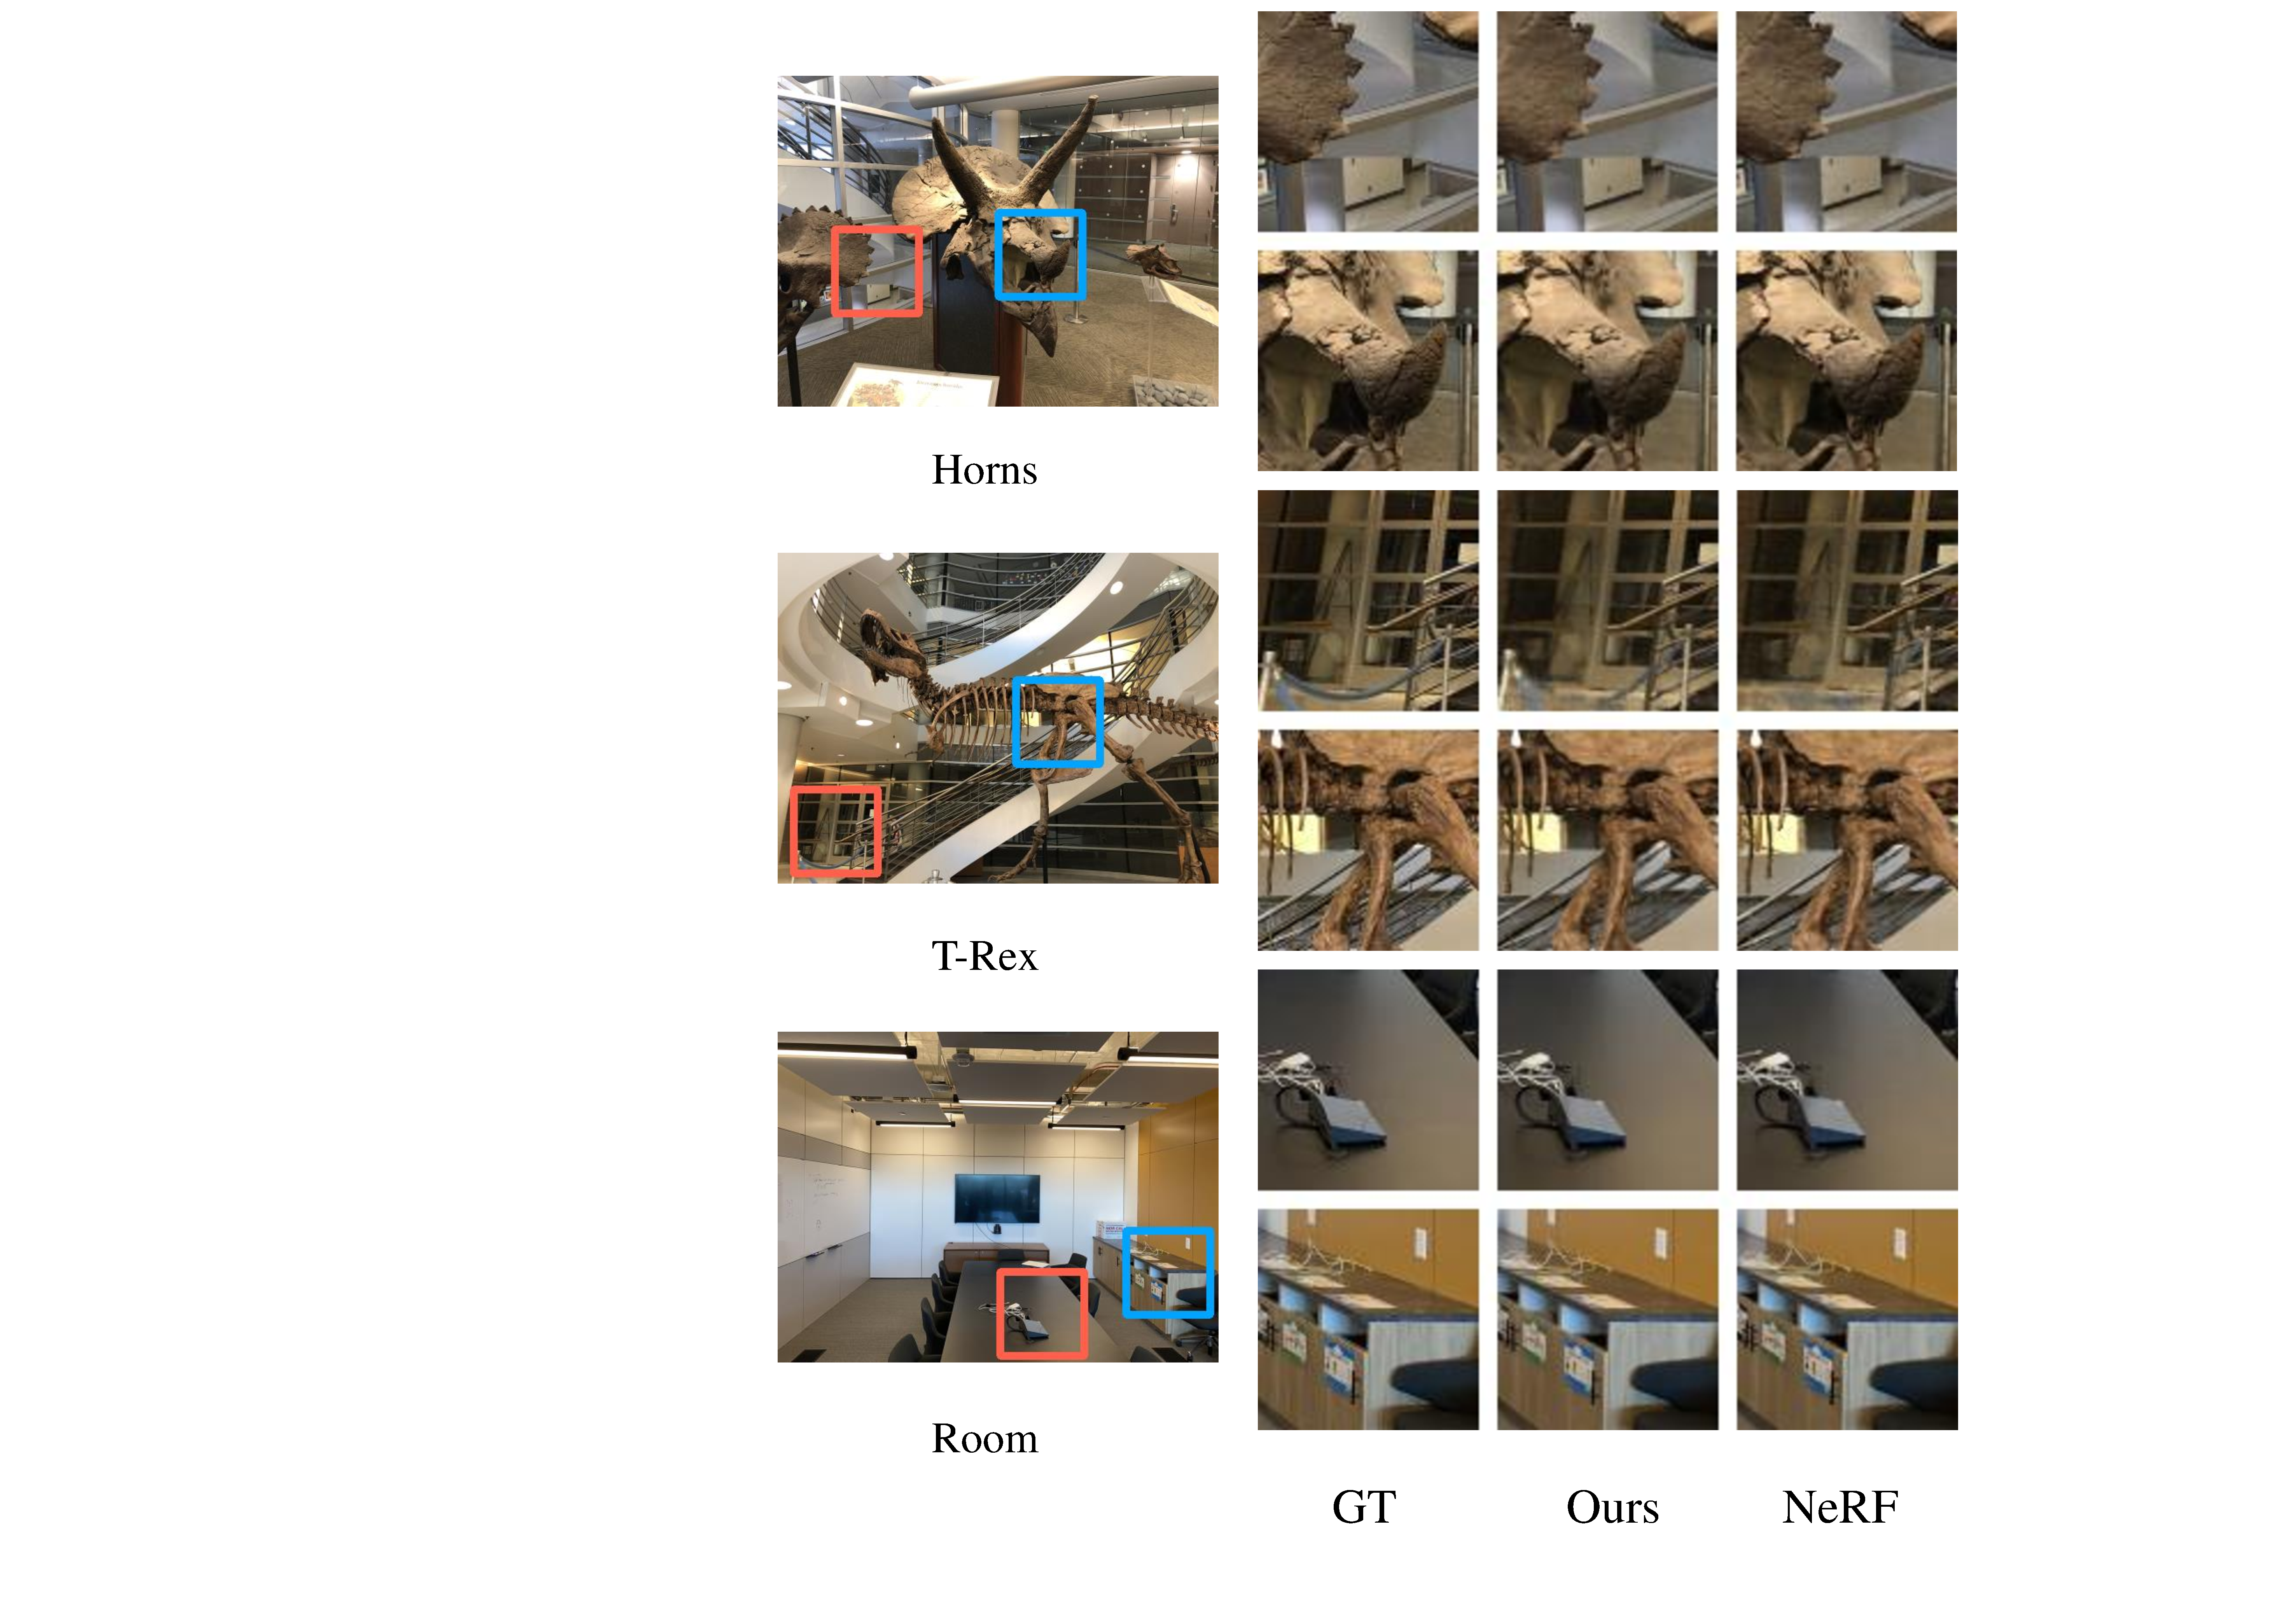
\includegraphics[width=0.95\textwidth]{figures/llff.pdf}
    \caption{F-NeRF 与 NeRF 在真实场景数据集 LLFF-NeRF 上的定性比较,使用的是分辨率为$504 \times 378$的图像。}
    \label{fig:llff}
\end{figure}
\newpage

\section{本章小结}
本章主要介绍了本文的实验部分。本章第~\ref{experiment-set} 节首先介绍了本文实验的开发环境、数据集。第~\ref{details} 节详细叙述了本文实验的一些细节,包括参数的设置,完整的训练过程,以及完整的测试过程。第~\ref{metrics} 节主要介绍了实验的具体评测指标,包含新视图合成任务中较为权威的质量评测指标,比如 PSNR、SSIM 和 LPIPS,这些指标涵盖了客观、结构相似性,以及人眼感知等多个维度去评估图像的质量,此外本节还提供了速度评估指标,主要是测试时间或渲染的帧率。最后分别基于公开的合成数据集 Synthetic-NeRF 和真实场景数据集 LLFF-NeRF, 将本文提出的方法与 NeRF 进行了性能对比,从结果上面看,本文提出的方法几乎在不损失质量的情况下对 NeRF 进行明显加速。

% \section{数学符号}

% 论文中使用的符号应符合国家标准《国际单位制及其应用》(GB 3100—1993)、《有关量、单位和符号的一般原则》(GB/T 3101—1993) 的规定。

% 要特别注意以下几点问题:

% \begin{enumerate}
% \item 数学公式结尾也不可缺少标点符号, 参见式\eqref{eq:example}, 式\eqref{eq:align}, 式\eqref{eq:equ_aligned}.
%     \item 向量、矩阵和张量要求粗斜体,应该使用 \pkg{unicode-math} 的 \cs{symbf} 命令,
%           如 \verb|\symbf{A}|、\verb|\symbf{\alpha}|。
%     \item 数学常数和特殊函数要求用正体,应使用 \cs{symup} 命令,
%     如 $\symup{\pi} = 3.14\dots$; $\symup{e} = 2.718\dots$。
%     \item 微分号和积分号使用使用正体,比如:$\int f(x) \dif x$。
%     \item 公式中的括号应写作 $\displaystyle \left(\frac{a}{b + c}\right)$, $\displaystyle \left[\frac{a}{b + c}\right]$, $\displaystyle \left\{\frac{a}{b + c}\right\}$, $\displaystyle \left<\frac{a}{b + c}\right>$, 而非 $\displaystyle (\frac{a}{b + c})$, $\displaystyle [\frac{a}{b + c}]$, $\displaystyle \{\frac{a}{b + c}\}$, $\displaystyle <\frac{a}{b + c}>$.\\
%     注意比较两种形式括号大小的区别. 在\LaTeX{}可用 \verb|\left(| $\cdot$ \verb|\right)|, \verb|\left[| $\cdot$ \verb|\right]|, \verb|\left\{| $\cdot$ \verb|\right\}|, \verb|\left<| $\cdot$ \verb|\right>| 来实现.
%     \item 关于量和单位推荐使用\href{http://mirrors.ctan.org/macros/latex/contrib/siunitx/siunitx.pdf}{\pkg{siunitx}}
% 宏包,
%         可以方便地处理希腊字母以及数字与单位之间的空白,
%         比如:
%         \SI{6.4e6}{m},
%         \SI{9}{\micro\meter},
%         \si{kg.m.s^{-1}},
%         \SIrange{10}{20}{\degreeCelsius}。
% \end{enumerate}

% \section{数学公式}

% 数学公式可以使用 \env{equation} 和 \env{equation*} 环境。
% 注意数学公式的引用应前后带括号,建议使用 \cs{eqref} 命令,比如式 \eqref{eq:example},
% \begin{equation}
%   \frac{1}{2 \symup{\pi} \symup{i}} \int_\gamma f = \sum_{k=1}^m n\left(\gamma; a_k\right) \mathscr{R}\left(f; a_k\right).
%   \label{eq:example}
% \end{equation}

% 多行公式尽可能在 ``='' 处对齐,可根据编号形式的需要使用 \env{align} 或 \env{equation}+\env{aligned} 环境, 请参考如下示例:

% \env{align}模式: 

% \begin{minipage}{.48\textwidth}
%     \begin{verbatim}
% \begin{align}
%   a & = b + c + d + e, \\
%     & = f + g.
% \end{align}
%     \end{verbatim}
% \end{minipage}
% \begin{minipage}{.48\textwidth}
%   \begin{align}\label{eq:align}
%     a & = b + c + d + e, \\
%       & = f + g.
%   \end{align}
% \end{minipage}

% \env{equation} + \env{aligned} 模式:

% \begin{minipage}{.48\textwidth}
%     \begin{verbatim}
% \begin{equation}
%     \begin{aligned}
%       a & = b + c + d + e, \\
%         & = f + g.
%     \end{aligned}
% \end{equation}
%     \end{verbatim}
% \end{minipage}
% \begin{minipage}{.48\textwidth}
%     \begin{equation}\label{eq:equ_aligned}
%         \begin{aligned}
%           a & = b + c + d + e, \\
%             & = f + g.
%         \end{aligned}
%     \end{equation}
% \end{minipage}

% \section{数学定理}

% 定理环境的格式可以使用 \pkg{amsthm} 或者 \pkg{ntheorem} 宏包配置。
% 用户在导言区载入这两者之一后,模板会自动配置 \env{thoerem}、\env{proof} 等环境。

% \begin{theorem}[Lindeberg--Lévy 中心极限定理]
%   设随机变量 $X_1, X_2, \dots, X_n$ 独立同分布, 且具有期望 $\mu$ 和有限的方差 $\sigma^2 \ne 0$,
%   记 $\bar{X}_n = \frac{1}{n} \sum_{i+1}^n X_i$,则
%   \begin{equation}
%     \lim_{n \to \infty} P \left(\frac{\sqrt{n} \left( \bar{X}_n - \mu \right)}{\sigma} \le z \right) = \Phi(z),
%   \end{equation}
%   其中 $\Phi(z)$ 是标准正态分布的分布函数。
% \end{theorem}
% \begin{proof}
%   Trivial.
% \end{proof}

% 同时模板还提供了 \env{assumption}、\env{definition}、\env{proposition}、
% \env{lemma}、\env{theorem}、\env{axiom}、\env{corollary}、\env{exercise}、
% \env{example}、\env{remar}、\env{problem}、\env{conjecture} 这些相关的环境。

\cleardoublepage

\cleardoublepage
% !TeX root = ../main.tex

\chapter{系统设计与实现}\label{figures_tables}
第三、四章分别对本文提出的“基于神经辐射场的快速新视图合成方法”的方法论的详述和在公开数据集上大量的实验对比验证。为了将上述研究方法转成实际的系统,本文设计并实现了基于神经辐射场的快速新视图合成系统。此系统可以接入移动端相机传感器采集的多视角的图像,再通过本文提出的方法训练出高保真的神经辐射场,最终可以快速渲染出任意新视角的视图,可以和已知位姿的 ground truth 进行对比。

\section{系统需求分析}

\subsection{功能性需求分析}\label{functional}
基于上一节提出的系统设计的思路,本文基于神经辐射场的新视图快速合成系统可分为两大模块,分别是数据处理模块和算法模块,具体见图~\ref{fig:system_struct}。
\begin{figure}[htbp]
    \centering
    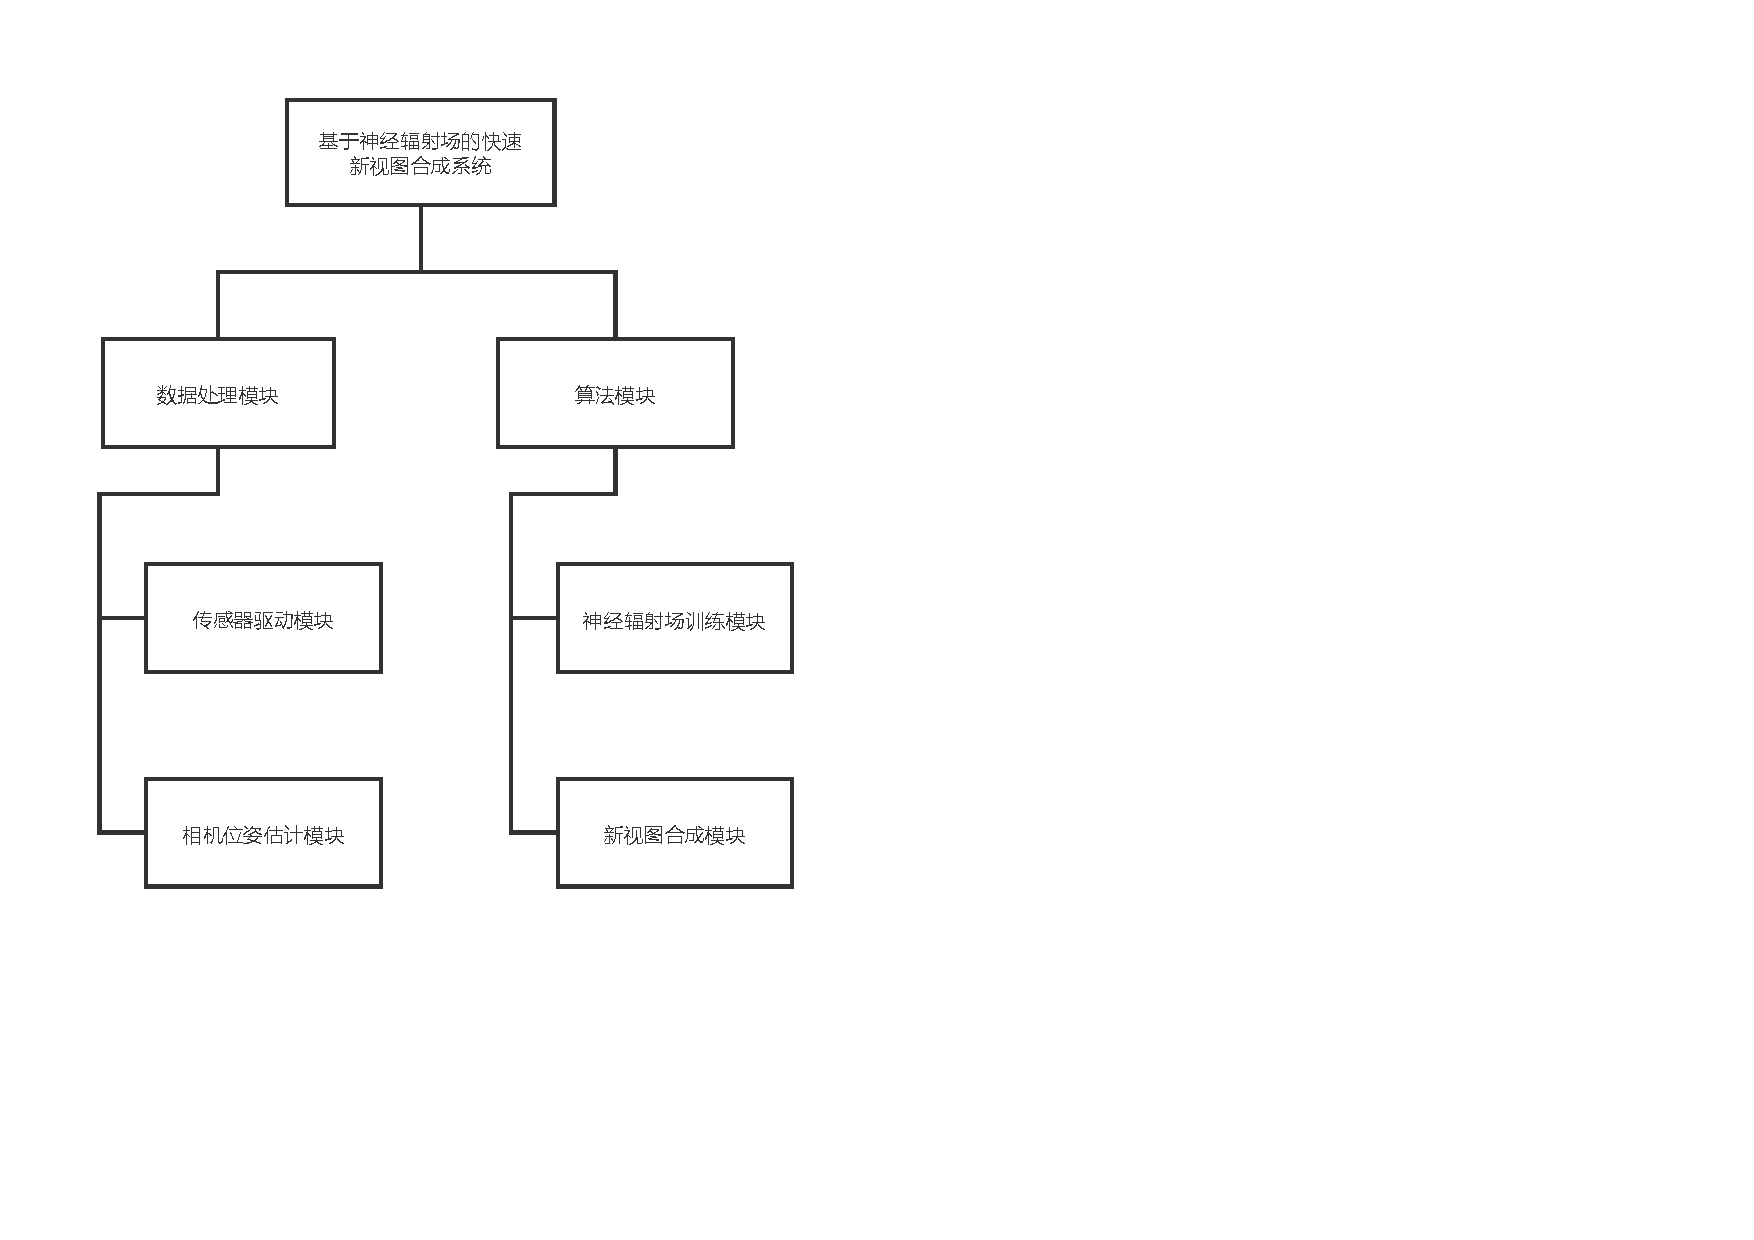
\includegraphics[width=0.65\linewidth]{figures/system_struct.pdf}
    \caption{系统功能结构图}
    \label{fig:system_struct}
\end{figure}

\begin{enumerate}
    \item [a)] 数据处理模块:包括以下两个模块内容:
               \begin{enumerate}
                   \item [1)] 传感器驱动模块:用于获取传感器的数据,例如 RGB 图像。
                   \item [2)] 相机位姿估计模块:使用 COLMAP \cite{schonberger2016structure} 实现对真实图像位姿的计算。
               \end{enumerate}
    \item [b)] 算法模块:包括以下两个模块内容:
               \begin{enumerate}
                   \item [1)] 神经辐射场训练模块:用于将已知位姿的图像训练成一个 5D 神经辐射场。
                   \item [2)] 新视图合成模块:通过训练好的模型,给定位姿,合成该位姿下的新视图。
               \end{enumerate}        
\end{enumerate}

\subsection{其他需求分析}
在经典的软件质量模型 “FURPS+” 中,除了上一小节的功能性需求,还剩下四个非功能性需求,分别是易用性 (Usability)、可靠性 (Reliability)、性能 (Performance) 还有可支持性 (Supportability)。使用 “FURPS+” 模型来实现需求分析可保障用户体验,比较好地能保证系统的运行质量。

以下是对本系统的非功能性需求进行分析:
\begin{enumerate}
    \item [a)] 易用性:在设计该系统的时候,系统的界面应该整洁美观,按钮名称应该通俗易懂,符合用户的操作习惯,降低用户的学习成本。
    \item [b)] 可靠性:系统应该足够鲁棒,能够处理各个模块中可能产生的异常,尽可能避免系统崩溃,如出现不可避免的错误应及时反馈给用户。     
    \item [c)] 性能:系统应在相关的平台上能流畅运行,系统的时延要能满足一般用户体验,本身应增加与用户交流的对话框,提高用户体验。此外,性能还体现在合成新视图的速度以及质量上,这是本文方法论所主要考量的指标。
    \item [d)] 可支持性:系统各功能模块清晰明确,模块之间应该是解耦的,方便日后维护、扩展、更新。接口命名以及教程足够清晰,方便其他开发者使用。
\end{enumerate}

\subsection{主要用例分析}
本小节主要介绍 PC 端的各个应用模块用例。

用户可以进行的操作包括与相机的交互,数据集的处理,以及新视图合成。用例图见图~\ref{fig:PCusercase}。

\pagebreak
\begin{figure}[htb]
	\centering
	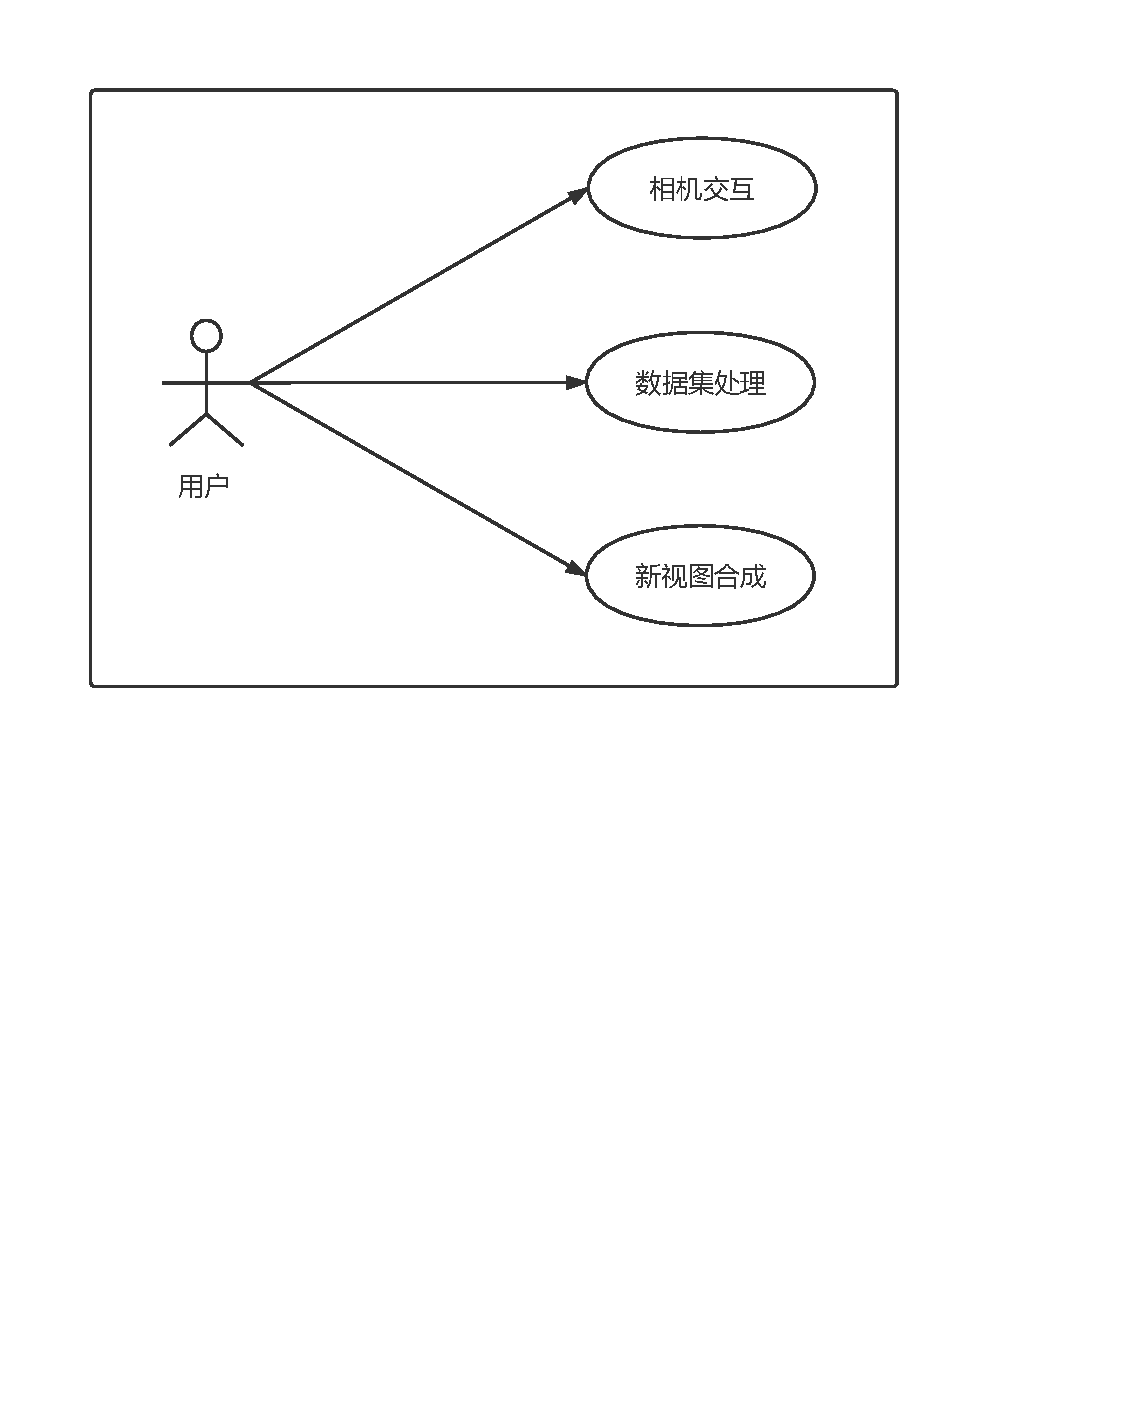
\includegraphics[width=0.55\linewidth]{figures/usercase.pdf}
	\caption{PC 客户端用例图}
	\label{fig:PCusercase}
\end{figure}

\begin{table*}
	\centering
	\small\def\arraystretch{0.91}\setlength\tabcolsep{0.05\textwidth}
	\caption{相机交互用例图User case\#1}
	\begin{tabular}{p{3.5cm}|p{8cm}}
		\hline
		用例编号 & User case\#1 \\
		\hline
		用例名 & 相机交互  \\
		\hline
		涉众及其关注点 & 用户:希望进行相机交互功能  \\
		\hline
		前置条件 & 用户启动应用 \\
		\hline
		主成功场景 & 1. 用户打开应用,点击“打开相机”按钮  \\
		& 2. 应用跳转至相机界面 \\
		& 3. 用户点击添加按钮 \\
		& 4.  当前相机画面被捕获到数据集栏并显示\\
		& 5.  用户点击“关闭相机”按钮\\
		&\quad 5a. 系统提示 “您确定要关闭相机吗?”  \\
		&\quad 5b. 系统保存用户处理结果,相机画面终止  \\
		& 6.  用户点击“退出系统”按钮\\
		&\quad 6a. 系统提示 “您确定要退出系统吗?”  \\
		&\quad 6b. 系统保存用户处理结果,整个应用退出  \\
		\hline
		拓展 & 5a. 相机关闭取消  \\	
		 & \quad 1. 交互界面保持不变  \\	
		     & 6a. 系统关闭取消  \\	
		& \quad 1. 交互界面保持不变  \\		
		\hline
		后置条件 & 应用显示相应处理结果 \\
		\hline
		发生频率 & 高 \\
		\hline
	\end{tabular}
	\label{tab:usercase1}
\end{table*}

\begin{table*}[thbp]
	\centering
	\small\def\arraystretch{1.5}\setlength\tabcolsep{0.05\textwidth}
	\caption{数据集处理用例图User case\#2}
	\begin{tabular}{p{3.5cm}|p{8cm}}
		\hline
		用例编号 & User case\#2 \\
		\hline
		用例名 & 数据集处理  \\
		\hline
		涉众及其关注点 & 用户:希望数据集处理功能  \\
		\hline
		前置条件 & 用户启动应用 \\
		\hline
		主成功场景 & 1. 用户打开应用,点击“打开相机”按钮  \\
		& 2. 应用跳转至相机界面 \\
		& 3. 用户点击添加按钮 \\
		& 4.  当前相机画面被捕获到数据集栏并显示\\
		& 5.  用户在数据集栏点击“上(下)一张”按钮\\
		& 6.  用户在数据集栏点击“删除”按钮\\
		&\quad 6a. 系统提示 “您确定删除吗?”  \\
		&\quad 6b. 系统保存用户处理结果,当前图像被删除  \\
		\hline
		拓展 & 3a. 添加数据集前未打开相机  \\	
		& \quad 1. 弹出提示框“请打开相机”  \\
		& 5a. 数据集为空  \\	
		& \quad 1. 弹出提示框“请添加图像至数据集”  \\
		& 6a. 点击取消删除或提示栏右上角$\times$  \\	
		& \quad 1. 数据集栏当前画面被保留  \\
		& 6b. 删除时,数据集为空$\times$  \\	
		& \quad 1. 弹出提示框“不可删除空数据”  \\	
		\hline
		后置条件 & 应用显示相应处理结果 \\
		\hline
		发生频率 & 高 \\
		\hline
	\end{tabular}
	\label{tab:usercase2}
\end{table*}

\begin{table*}[thbp]
	\centering
	\small\def\arraystretch{1.7}\setlength\tabcolsep{0.05\textwidth}
	\caption{新视图合成用例图User case\#3}
	\begin{tabular}{p{3.5cm}|p{8cm}}
		\hline
		用例编号 & User case\#3 \\
		\hline
		用例名 & 新视图合成  \\
		\hline
		涉众及其关注点 & 用户:希望执行新视图合成功能  \\
		\hline
		前置条件 & 用户启动应用 \\
		\hline
		主成功场景 & 1. 用户点击“计算位姿”按钮  \\
		& 2. 进度条提示计算位姿的过程 \\
		& 3. 用户点击“训练模型”按钮 \\
		& 4.  进度条提示模型训练的过程\\
		& 5.  用户点击“合成新视图”按钮\\
	    & 6. 状态提示从“待合成”到“合成中”再到“已合成” \\
	    & 7. 用户在数据集栏点击“上(下)一张”按钮 \\
		\hline
		拓展 & 1a. 计算位姿时,数据集为空:  \\	
		& \quad 1.   弹出提示框:“数据集不能为空”\\
		& 3a. 训练模型时,位姿为空:  \\	
		& \quad 1.   弹出提示框:“请先计算位姿”\\
		& 5a. 训练模型时,未训练模型:  \\	
		& \quad 1.   弹出提示框:“请先训练模型”\\		
		\hline
		后置条件 & 应用显示相应处理结果 \\
		\hline
		发生频率 & 高 \\
		\hline
	\end{tabular}
	\label{tab:usercase3}
\end{table*}

\pagebreak	
\section{系统设计}

\subsection{系统架构设计}
本文提出的神经辐射场的新视图快速合成系统主要分为三个部分,包含界面层、业务层、数据层。其中,界面层主要是为用户提供可视化的应用界面以方便用户进行相应的操作。业务层提供了本系统的所有业务基本操作,包括传感器驱动、位姿估计、神经辐射场训练、新视图合成。数据层负责数据库的管理和数据的控制,通过相机获取一系列 RGB 图像,并传给业务层去处理下游任务。本文系统是基于 Windows 平台的应用,对应的 PC 客户端使用 matlab 的 App Design 工具箱实现,具体的系统架构如图~\ref{fig:symtem_design} 所示。

\begin{figure}[htbp]
	\centering
	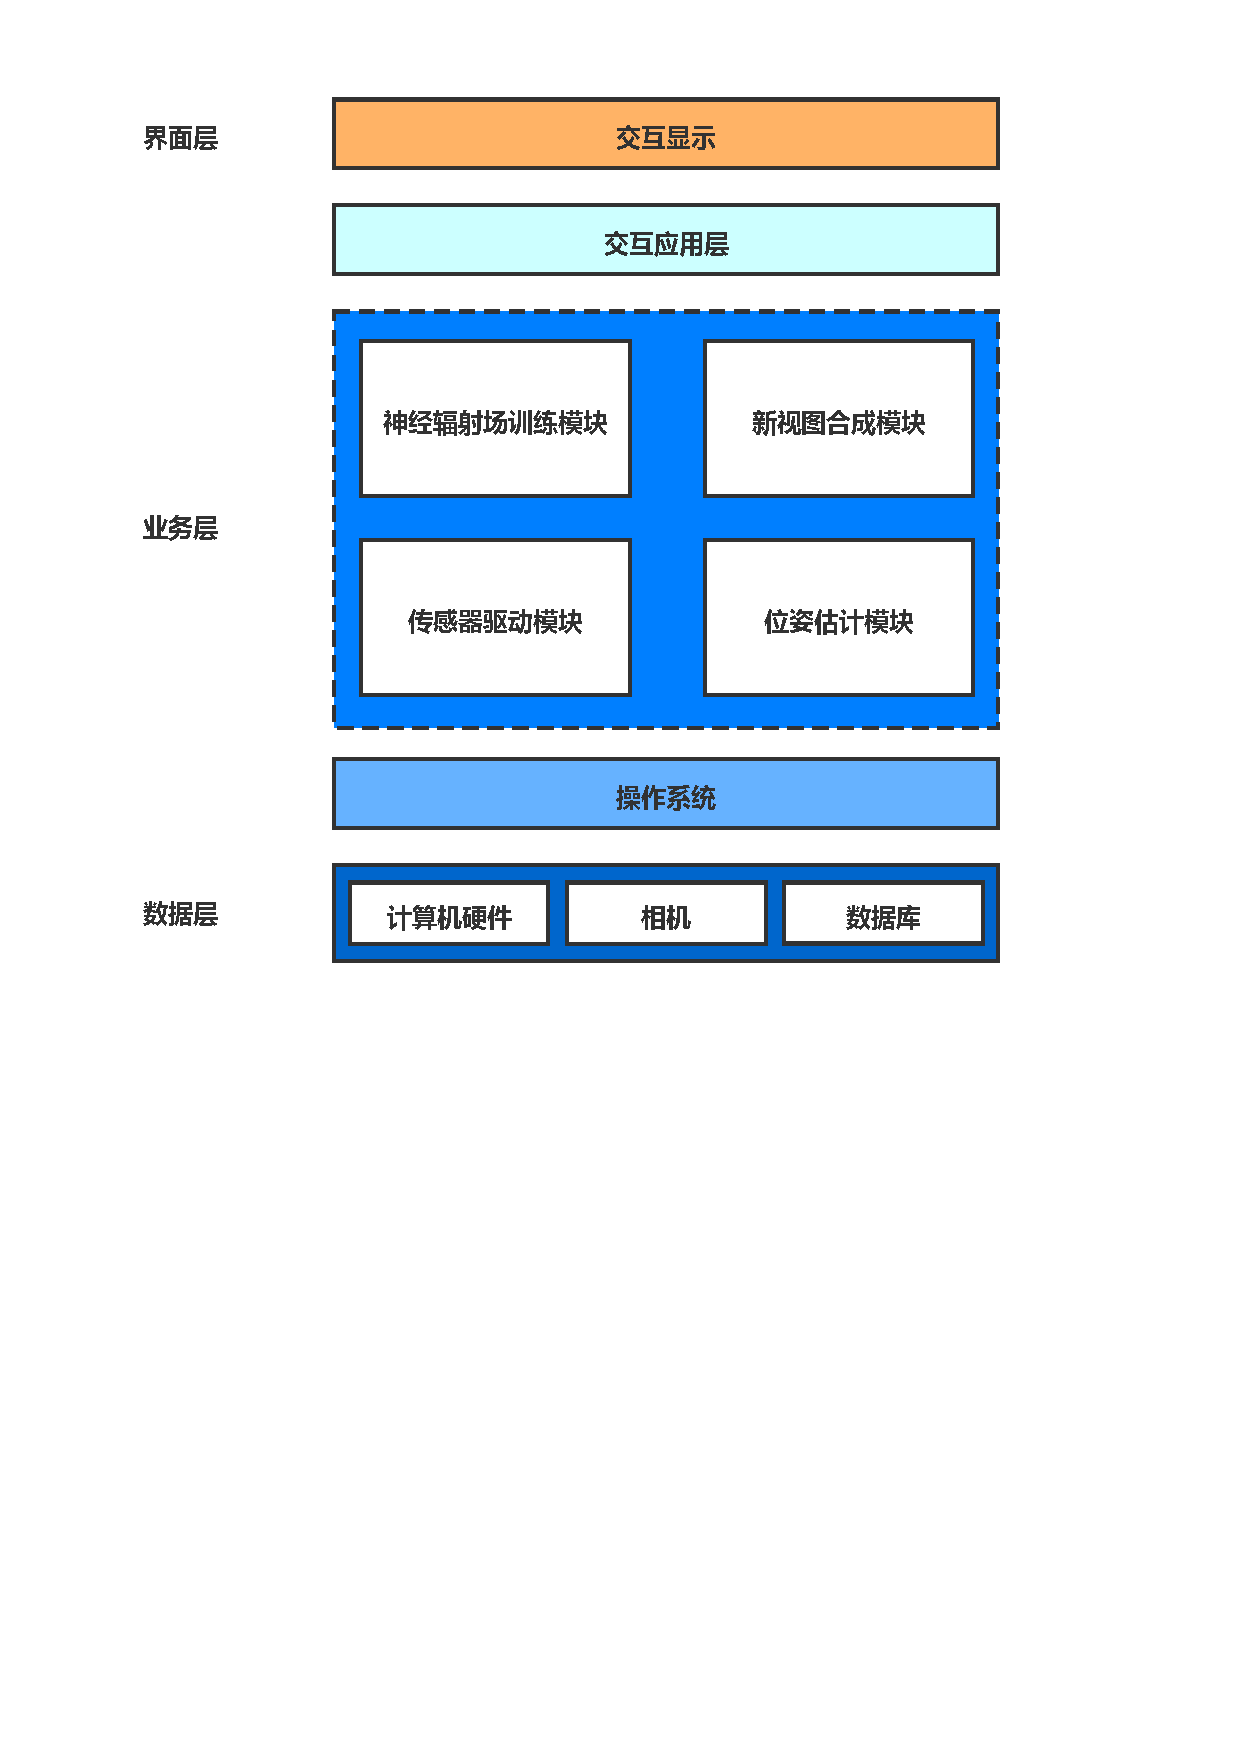
\includegraphics[width=0.75\linewidth]{figures/system_design_revised.pdf}
	\caption{系统架构示意图}
	\label{fig:symtem_design}
\end{figure}

\subsection{关键用例实现}
\subsubsection{相机交互}
相机交互功能的具体交互流程如下:
\begin{enumerate}
	\item 用户点击“打开相机”按钮,系统通过 MainWindow 激活 SensorDrive ,打开相机。
	
	\item 用户点击“添加”按钮,系统通过 SensorDrive 捕获实时的相机画面,一方面将调用 SensorDrive 的方法 addViewClicked,另一方面将该画面返回 MainWindow 并显示。
	\item 用户点击“关闭相机”按钮,系统通过 SensorDrive 关闭相机,并显示在 MainWindow 上。 
\end{enumerate}

图~\ref{fig:cameraSD} 是相机交互的顺序图,描述了上述交互流程。

\begin{figure}[htbp]
	\centering
	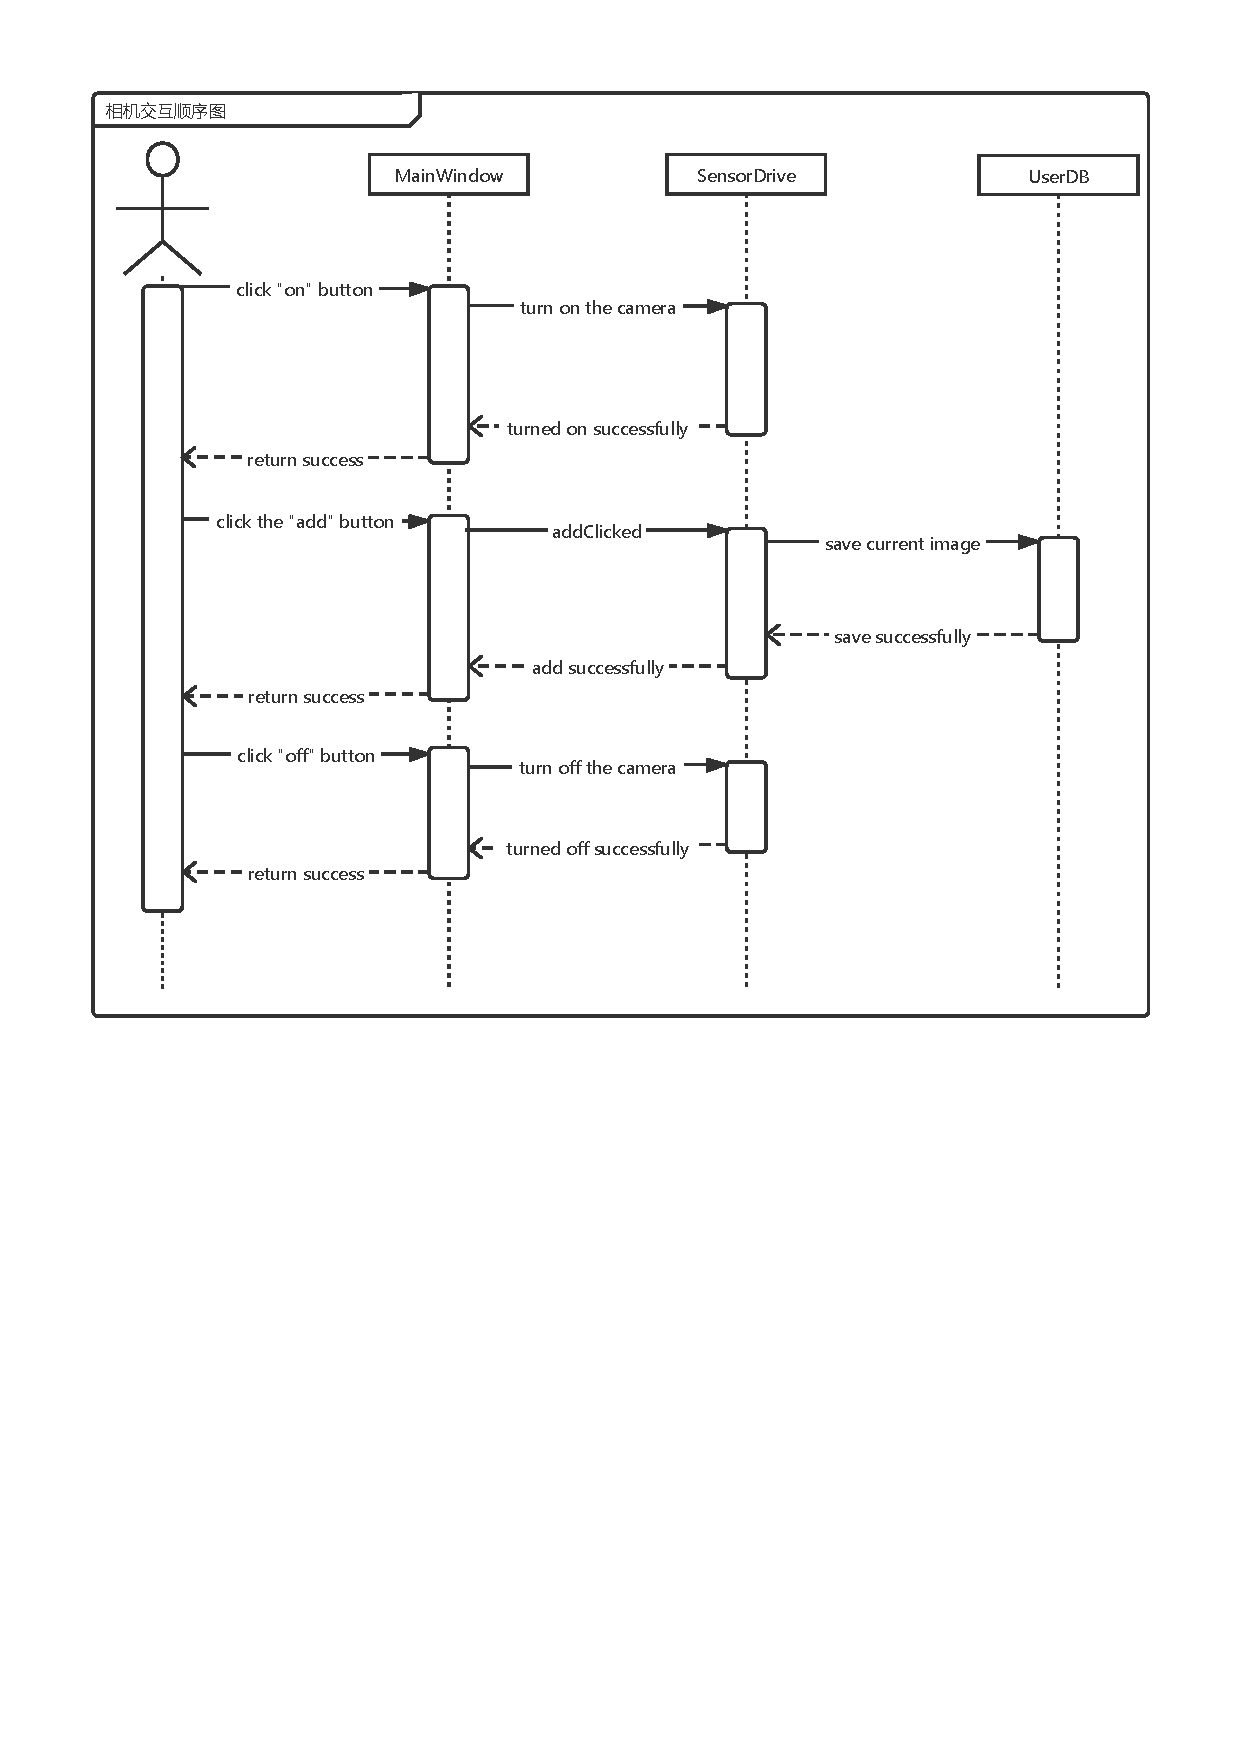
\includegraphics[width=0.85\linewidth]{figures/cameraSD.pdf}
	\caption{相机交互顺序图}
	\label{fig:cameraSD}
\end{figure}

\subsubsection{数据集处理}

\begin{enumerate}
	\item 用户点击“打开相机”按钮,系统通过 MainWindow 激活 SensorDrive ,打开相机。
	
	\item 用户点击“添加”按钮,系统通过 SensorDrive 捕获实时的相机画面,一方面将调用 SensorDrive 的方法 addViewClicked,另一方面将该画面返回 MainWindow 并显示。
	
	\item 用户点击“上/下一张”按钮,系统调用 UserDB 中的接口 lastClicked/nextClicked,系统将结果返回 MainWindow。
	
	\item 用户点击“删除”按钮,系统调用 UserDB 中的接口 deleteClicked,系统将结果返回 MainWindow。
\end{enumerate}

\begin{figure}[htbp]
	\centering
	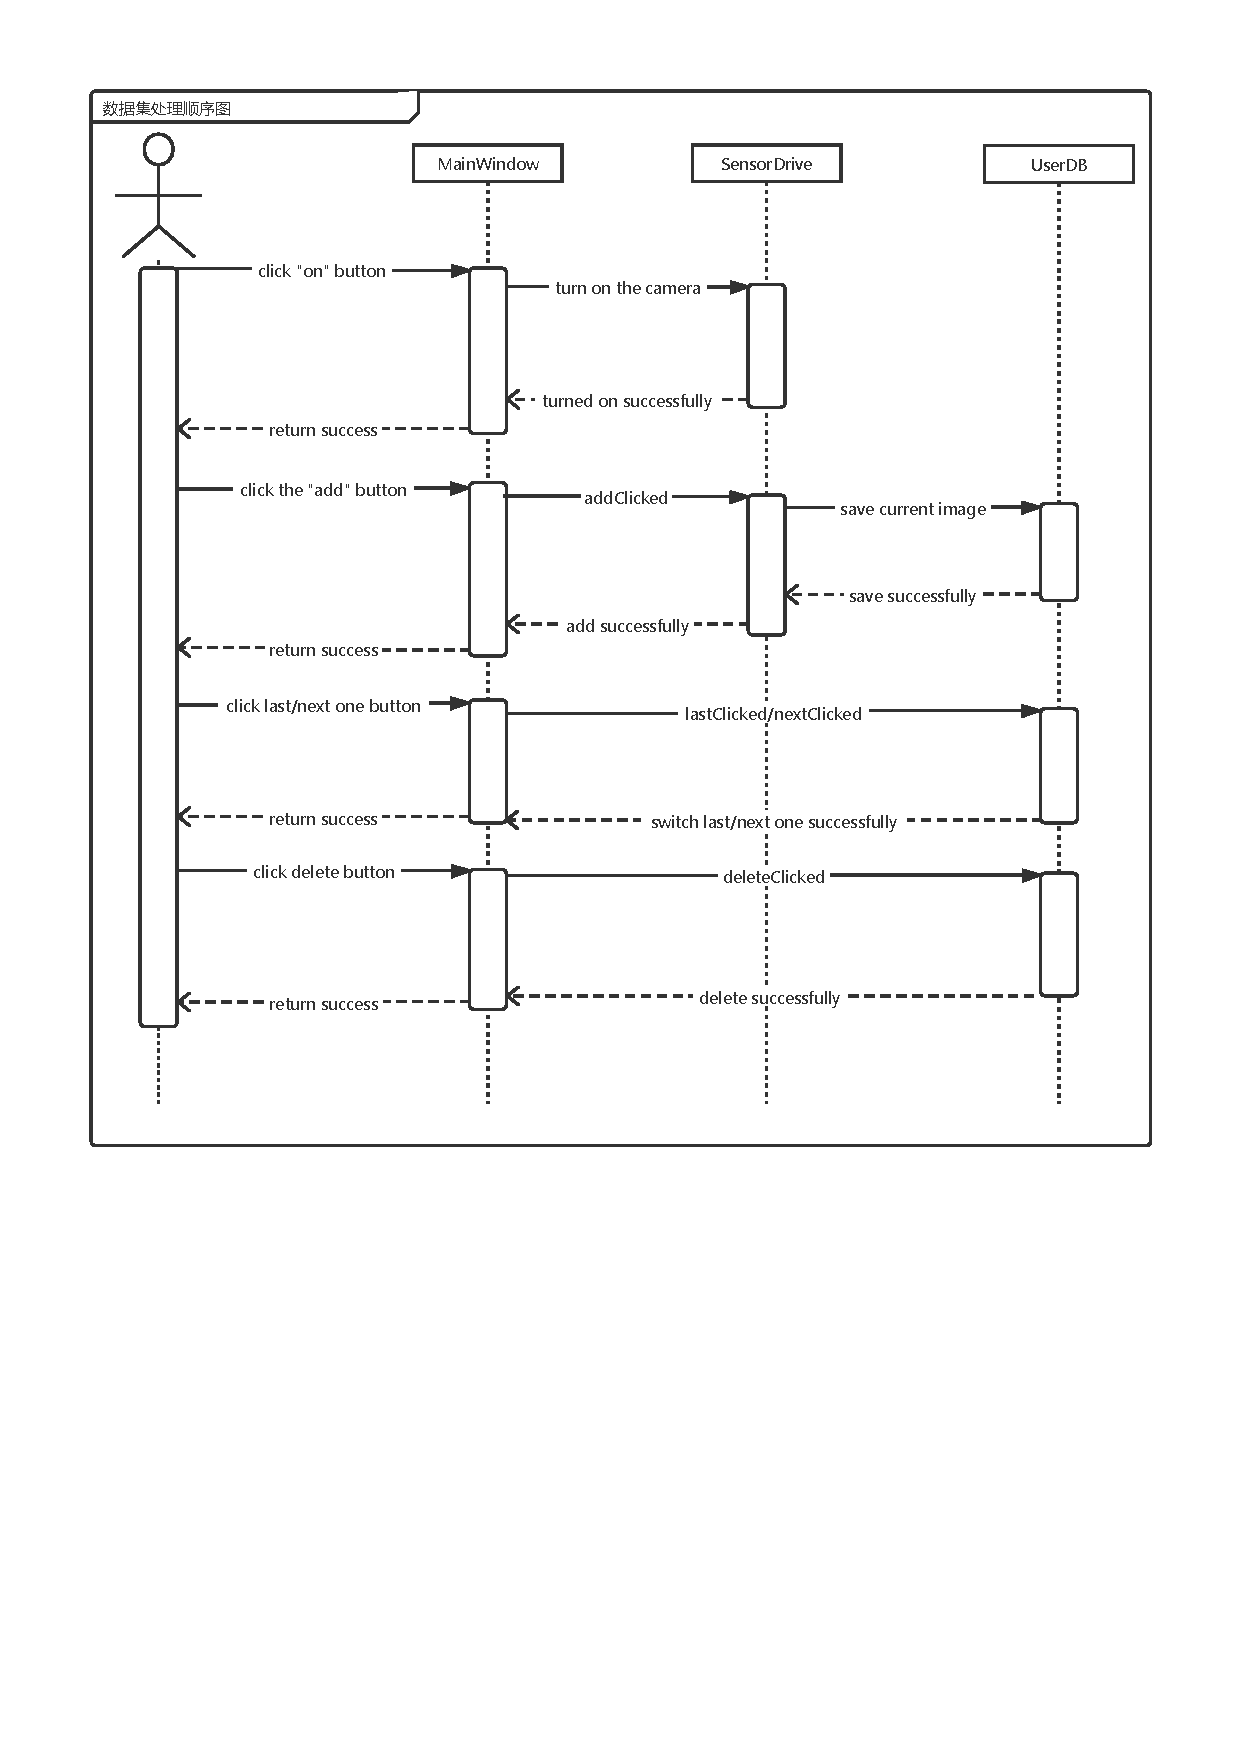
\includegraphics[width=0.85\linewidth]{figures/datasetProcessSD.pdf}
	\caption{数据集处理顺序图}
	\label{fig:datasetProcessSD}
\end{figure}

图~\ref{fig:datasetProcessSD} 是数据集处理的顺序图,描述了上述交互流程。

\subsubsection{新视图合成}
\begin{enumerate}
	\item 用户点击“计算位姿”按钮,系统通过 calPosesClicked 激活 FNeRF,打开相机。
	
	\item 用户点击“训练模型”按钮,系统通过 trainNeRFClicked 激活 FNeRF 使之向 UserDB 请求相应的数据并开始训练,训练过程进度条将显示在 MainWindow 上。
	
	\item 用户点击“合成新视图”按钮,系统通过 synViewsClicked 激活 FNeRF 使之向 UserDB 请求相应网络参数并开始渲染新视图,合成完毕信息将显示在 MainWindow 上。
\end{enumerate}

\begin{figure}[htbp]
	\centering
	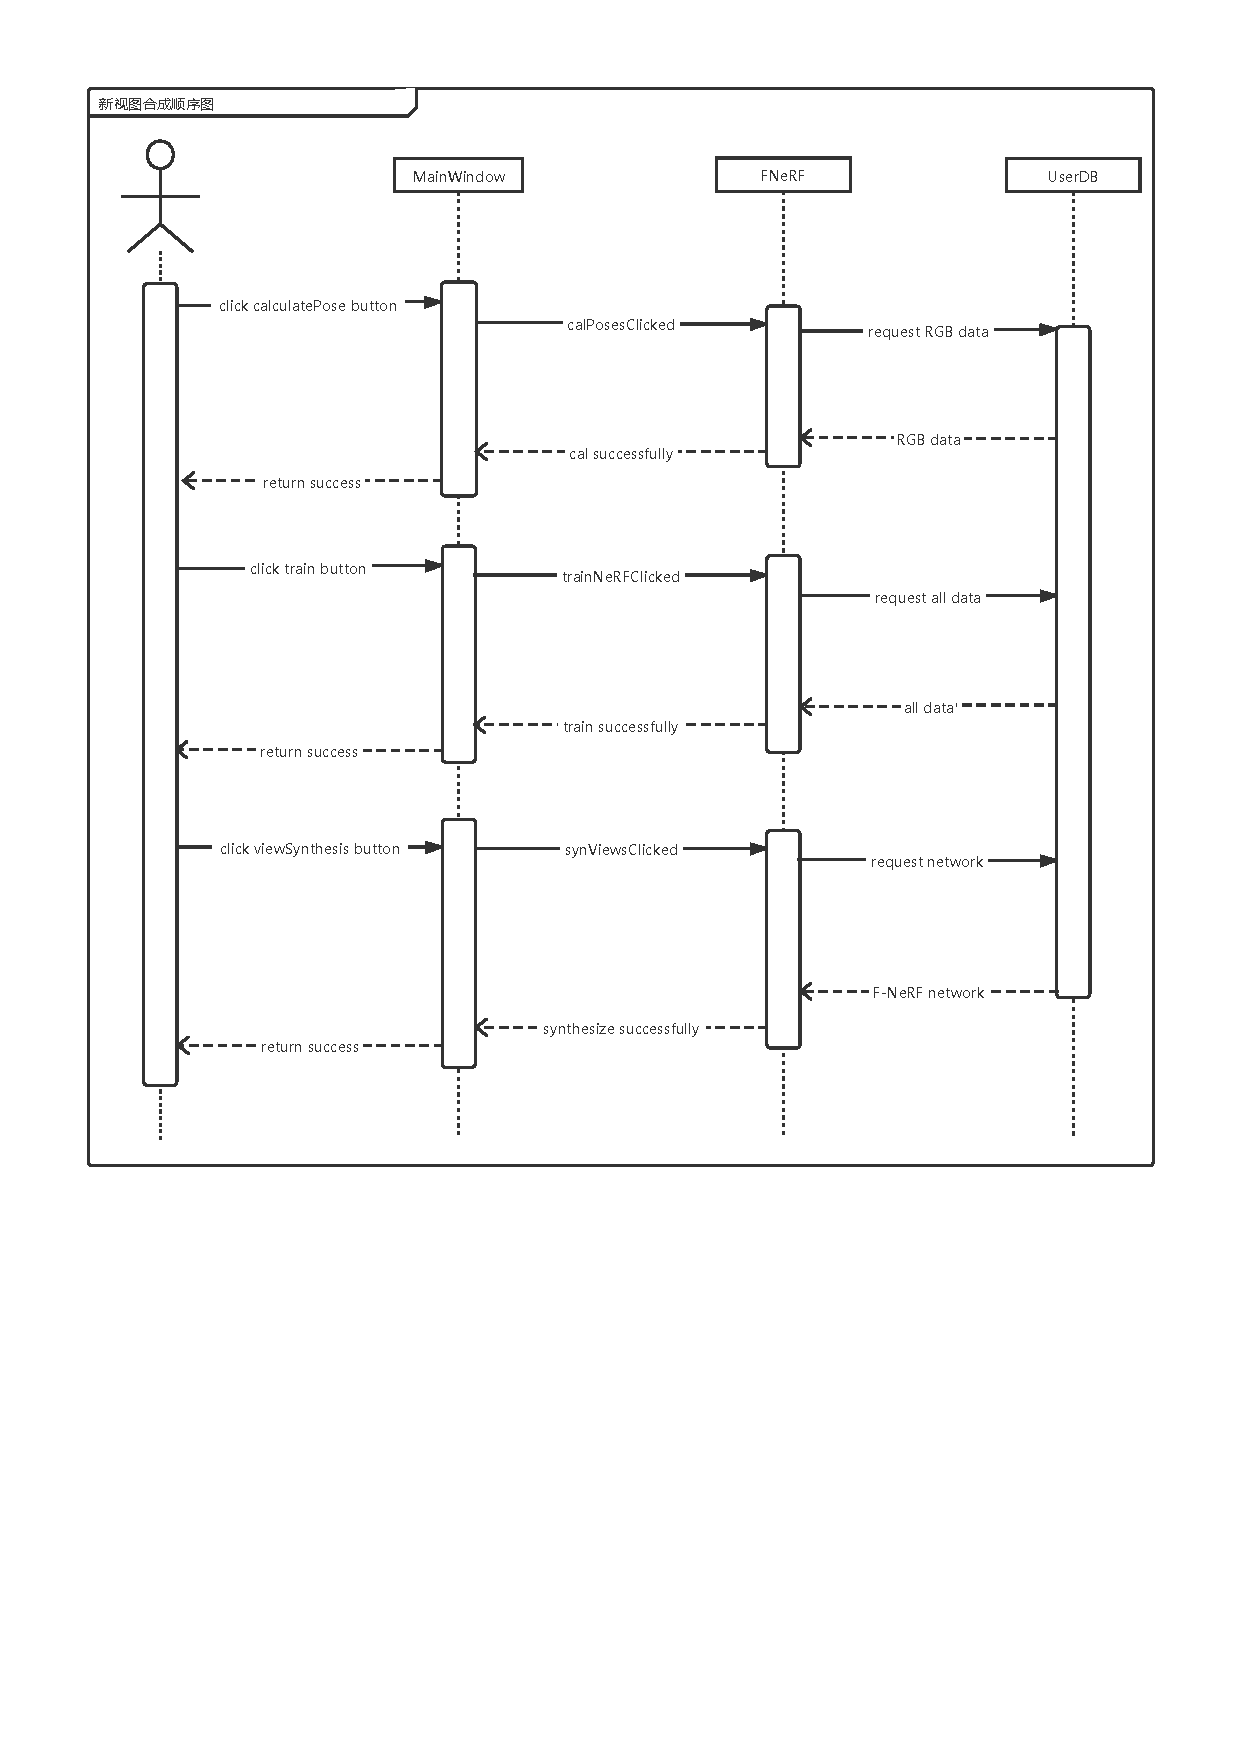
\includegraphics[width=0.85\linewidth]{figures/viewSynthesisSD.pdf}
	\caption{新视图合成顺序图}
	\label{fig:viewSynthesisSD}
\end{figure}

图~\ref{fig:viewSynthesisSD} 是新视图合成的顺序图,描述了上述交互流程。

\pagebreak
\subsection{模块详细设计}
\subsubsection{整体模块结构}
本系统主要由传感器驱动模块、位姿估计模块、神经辐射场训练模块以及新视图合成模块组成。这些模块的基本功能在第~\ref{functional} 小节已经简要叙述。
\subsubsection{传感器驱动模块}
传感器驱动模块实际上在本文中指的是相机模块,用以获取传感器的数据例如 RGB 图像,具体的类图如图~\ref{fig:sensorDriveCD} 所示。其中,MainActivity 为用户操作的主页面类,SensorActivity 为传感器操作类,ViewObject 封装了包含图像、位姿等信息的类。在 MainActivity 中打开相机后,系统调用 SensorActivity 的方法 addViewClicked 以捕获当前相机的画面,并通过 sendImage 在主界面显示当前捕获的图像,并将该图像存储在 UserDB 中。
\begin{figure}[htbp]
	\centering
	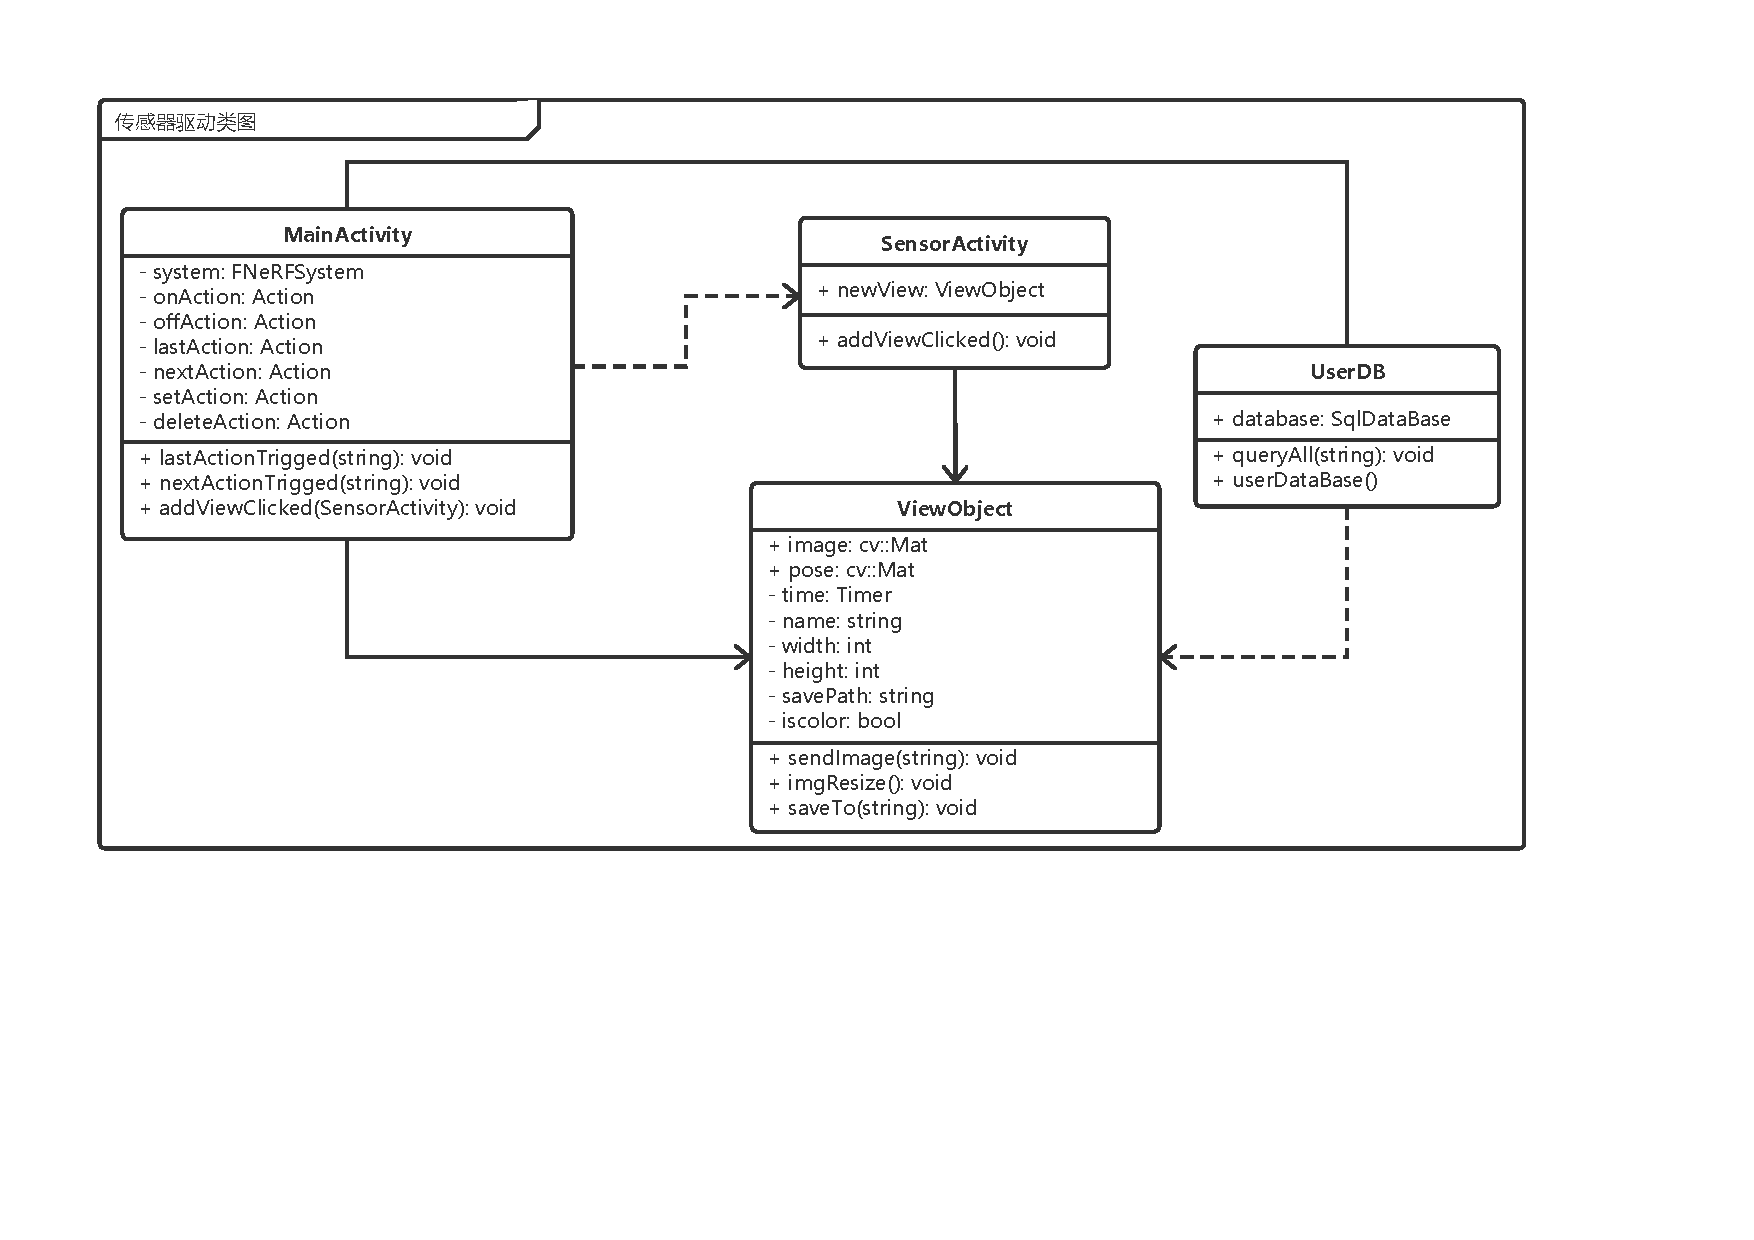
\includegraphics[width=0.95\linewidth]{figures/sensorDriveCD.pdf}
	\caption{传感器驱动类图}
	\label{fig:sensorDriveCD}
\end{figure}
\pagebreak
\subsubsection{位姿估计模块}
位姿估计模块在本系统中起着预处理数据的作用,调用 COLMAP\cite{schonberger2016structure} 算法的接口根据原始采集的 RGB 数据估计出相机位姿。

按照位姿估计模块的需求,构建了如图~\ref{fig:poseEstimationCD} 所示的类图以及方法。其中,PoseEstimator 为位姿估计模块对应的类,FNeRFSystem 为本系统各模块合并的类。通过 PoseEstimator 加载原始采集的 RGB 数据,并调用 COLMAP 的接口对位姿进行估计,之后将计算结果保存至数据库 UserDB。
\begin{figure}[htbp]
	\centering
	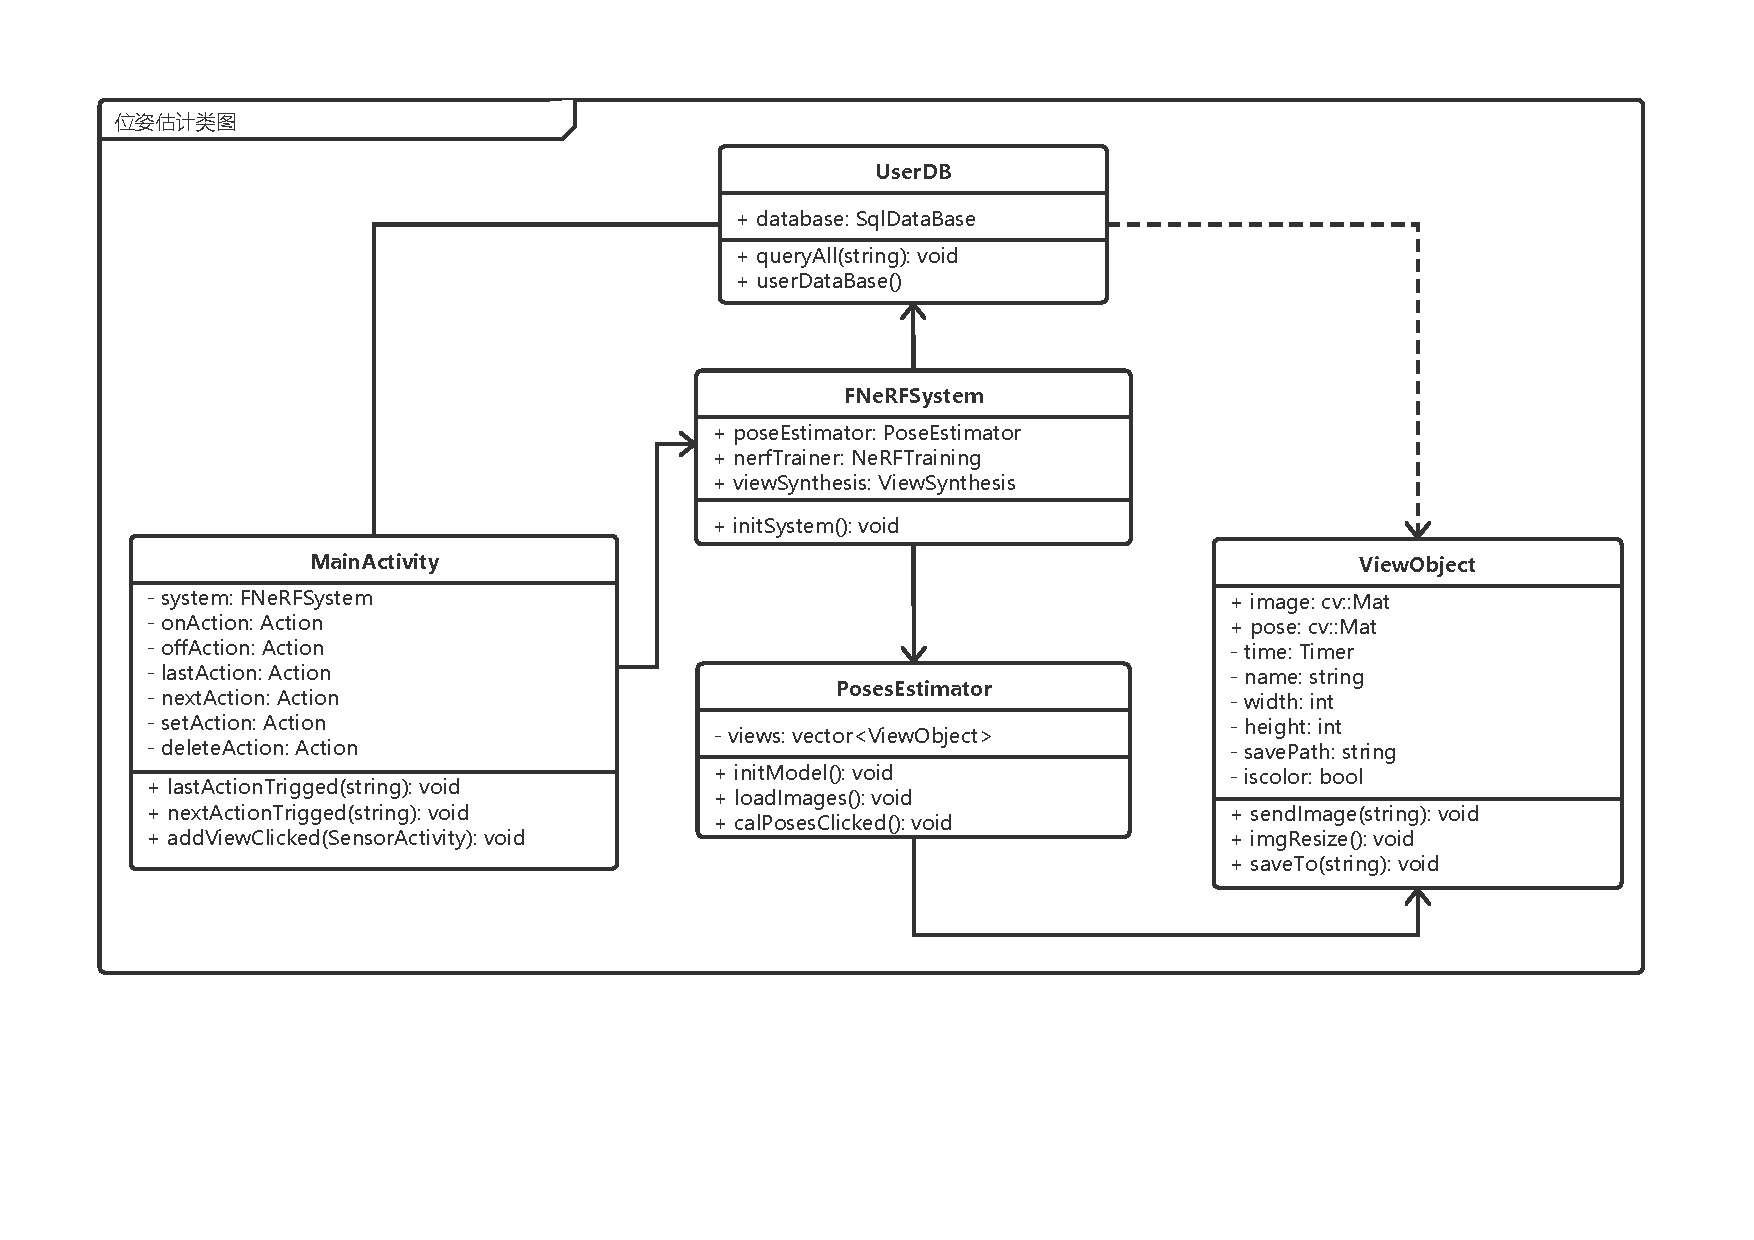
\includegraphics[width=0.95\linewidth]{figures/poseEstimationCD.pdf}
	\caption{位姿估计类图}
	\label{fig:poseEstimationCD}
\end{figure}

\subsubsection{神经辐射场训练模块}
神经辐射场训练模块实际上是使用本文第三章提出的基于神经辐射场的快速新视图合成算法对估计了位姿后的数据集进行训练,训练完毕后会保存神经网络的相关参数,便于后续快速新视图合成的测试。

根据神经辐射场训练模块的需求,构建了如图~\ref{fig:NeRFTrainCD} 所示的类图,NeRFTraining 为训练过程对应的类。通过 NeRFTraining 可以加载数据集并进行神经辐射场的训练,在训练过程中和训练完毕后都会保存相应的网络参数,便于测试时使用。
\begin{figure}[htbp]
	\centering
	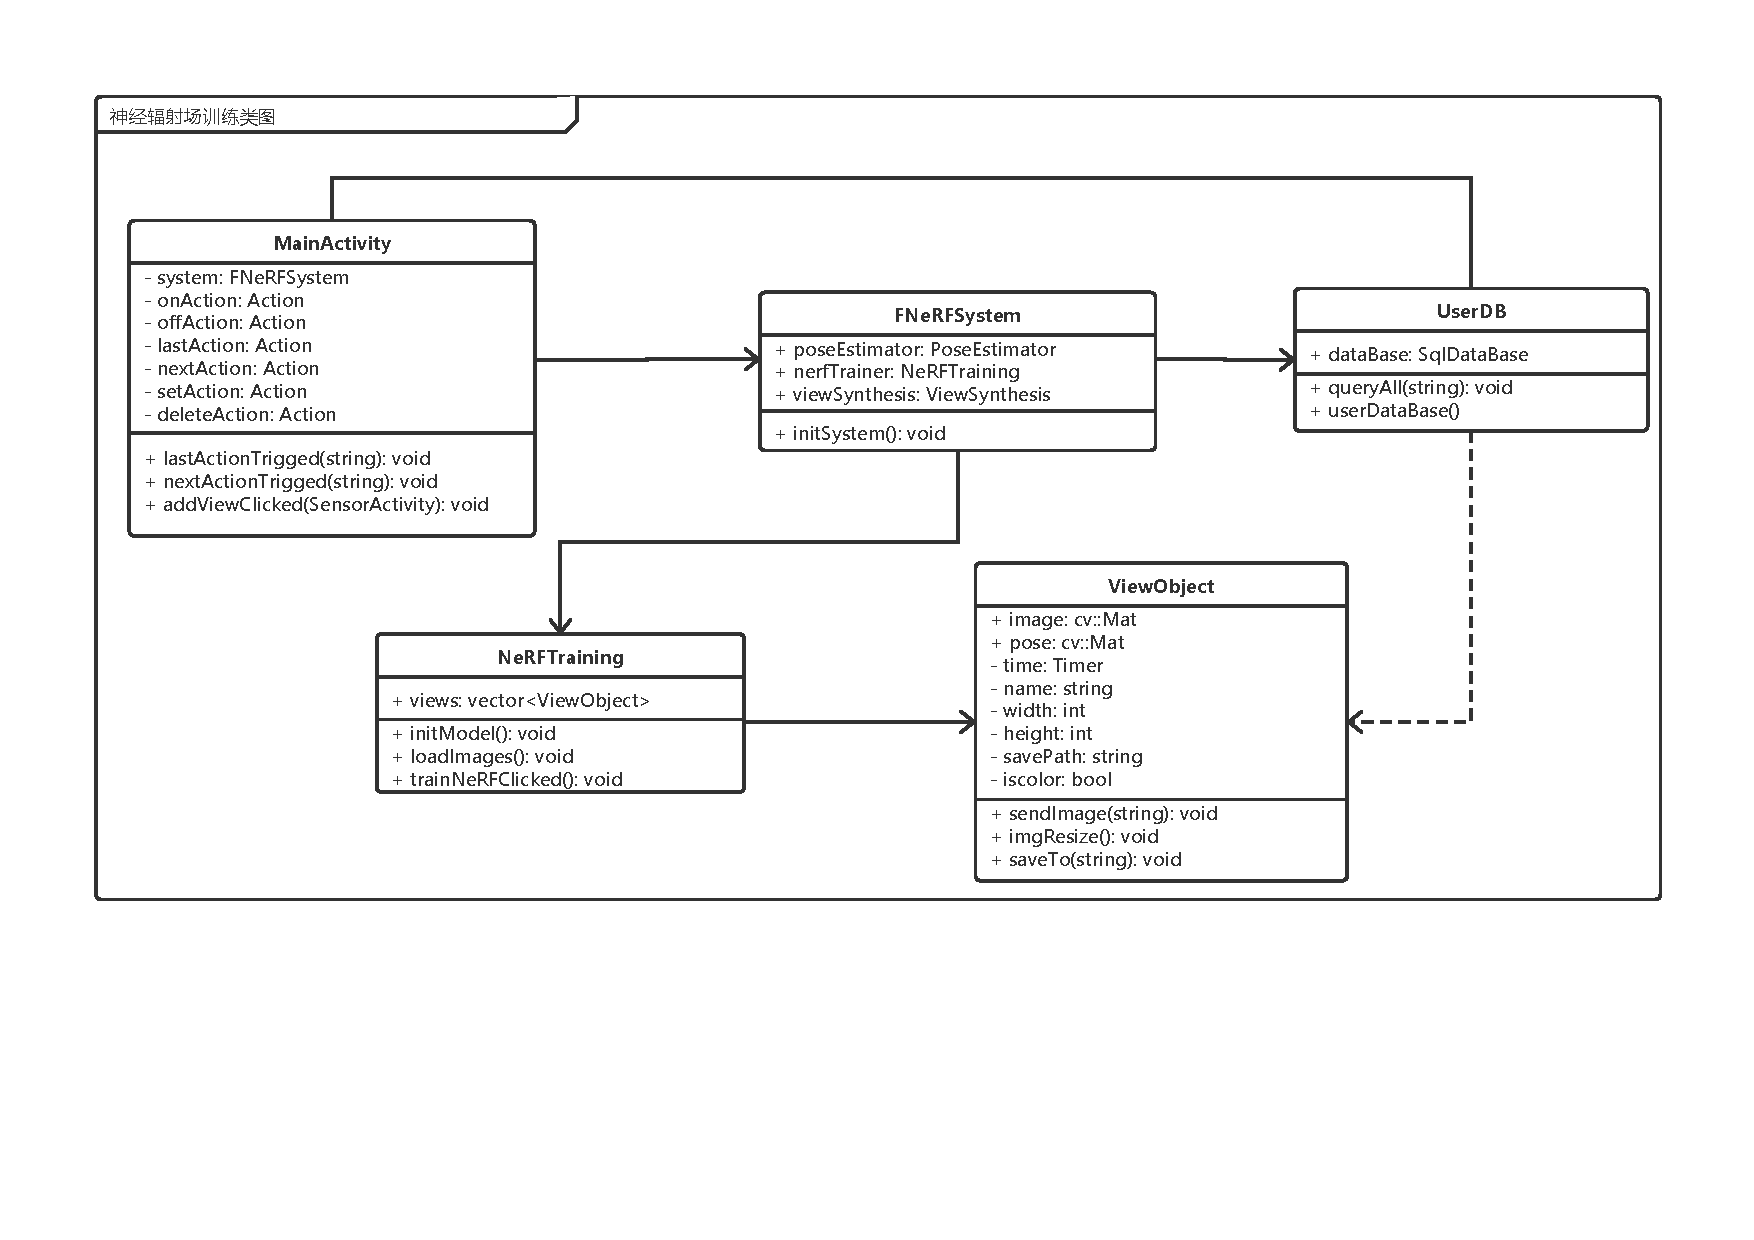
\includegraphics[width=0.95\linewidth]{figures/NeRFTrainCD.pdf}
	\caption{神经辐射场训练类图}
	\label{fig:NeRFTrainCD}
\end{figure}
\subsubsection{新视图合成模块}
新视图合成模块也是本系统的最后一个模块,负责使用训练好的神经辐射场(即 F-NeRF)快速合成新视角下的图像。

如图~\ref{fig:viewSynthesisCD} 所示的是新视图合成的类图,ViewSynthesis 对应着合成新视图的类。实际中,在测试之前需要提前加载好新视角下的位姿,然后使用 ViewSynthesis 中的 synViewClicked 方法通过训练好的 F-NeRF 网络合成新视图,并将新视图的质量和速度评价指标打印到主窗口上。
\begin{figure}[htbp]
	\centering
	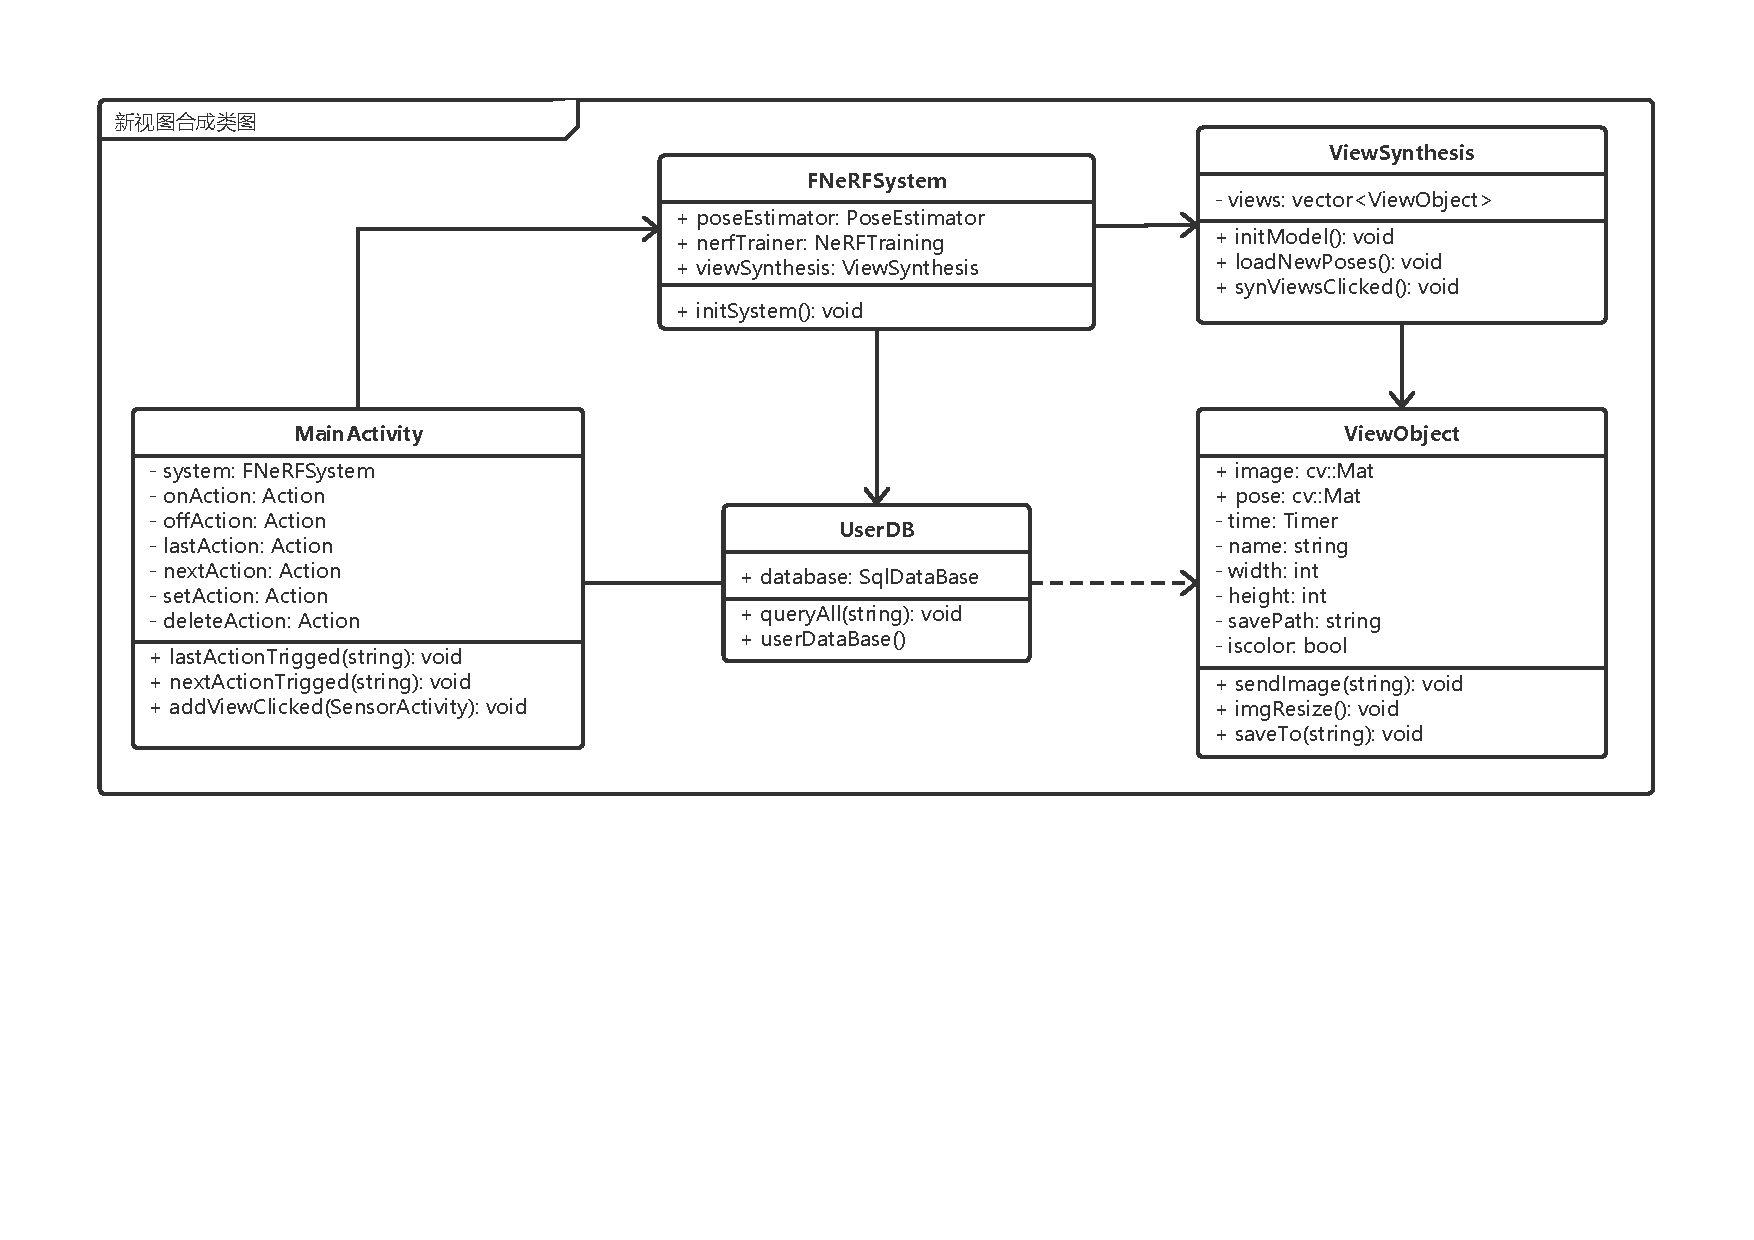
\includegraphics[width=0.95\linewidth]{figures/viewSynthesisCD.pdf}
	\caption{新视图合成类图}
	\label{fig:viewSynthesisCD}
\end{figure}

\subsection{主要技术细节实现}
本文设计并实现的基于神经辐射场的快速新视图合成系统是基于 Windows 平台开发,算法模块和数据处理模块均是基于 C++ 语言编写,用户交互界面是基于 matlab 语言编写。C++ 和 matlab 语言之间靠动态链接库进行数据通信。由于本文使用的基于神经辐射场的新视图快速合成模型是基于 Pytorch 框架训练的,而移动传感器调用代码使用的则是 C++ 语言,为了联合开发,需要引入 Pytorch 中的 torch.jit API 用来转换成 C++ 语言支持的模型文件上。

数据处理模块的位姿估计模块是基于开源的 COLMAP 框架去估计真实世界图像的位姿的,当然这不会像合成数据集那样有绝对准确的位姿,质量这一部分势必会下降,但位姿的优化不是本文所研究的问题,在此不作过多阐述。接下来将详细介绍本文快速新视图合成算法模块的 Pytorch 模型是如何移植到 C++ 代码上的,需要使用到 LibTorch 库。

Pytorch 是 Facebook 于2007年开发的当今最流行的深度学习框架之一。它有许多优点,比如底层使用 C++ 语言编写,有类似于 numpy 的张量计算,可以用于 GPU 加速,并且支持动态图,编写调试灵活,深受深度学习开发人员的青睐。为了将 pytorch 训练好的模型能够方便地迁移到 C++ 代码中,需要使用 Pytorch 的 C++ API 模型文件 LibTorch。模型转换加载的过程如下: 

\begin{enumerate}
    \item 首先是模型转换,创建与模型相同的随机张量,使用 torch.jit.trace 模块对运算过程和权值进行跟踪和捕获,进而序列化为 LibTorch 可以加载的模型文件。
    \item 下载对应平台预编译好的 LibTorch 库,添加 include 和 lib 目录
到编译环境中。
    \item 在 C++ 代码中加载转换后的 Pytorch 模型即可调用。 
\end{enumerate}

%\begin{figure}[htb]
%    \centering
%    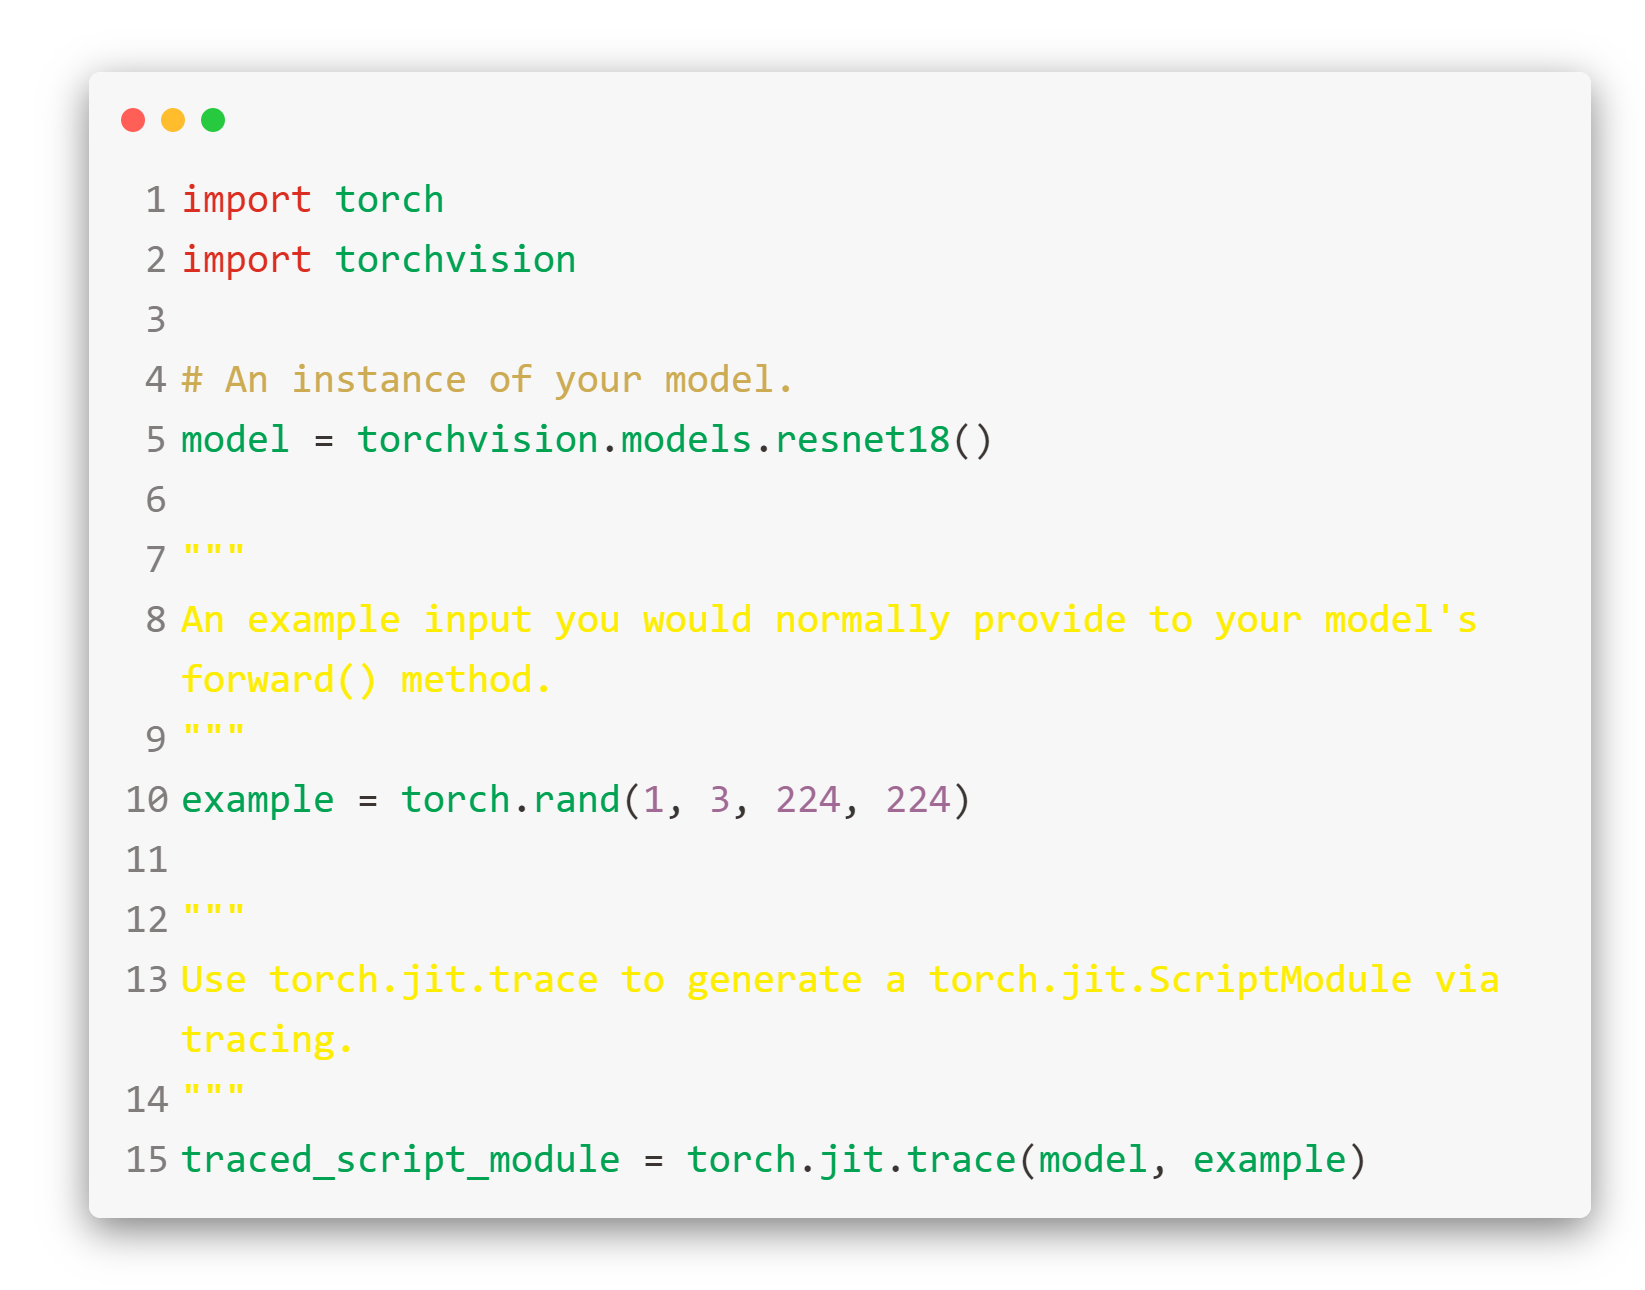
\includegraphics[width=0.98\linewidth]{figures/code-pytorch-big.png}
%    \caption{Pytorch 模型的转换}
%    \label{fig:code_pytorch}
%\end{figure}
%
%\begin{figure}[H]
%    \centering
%    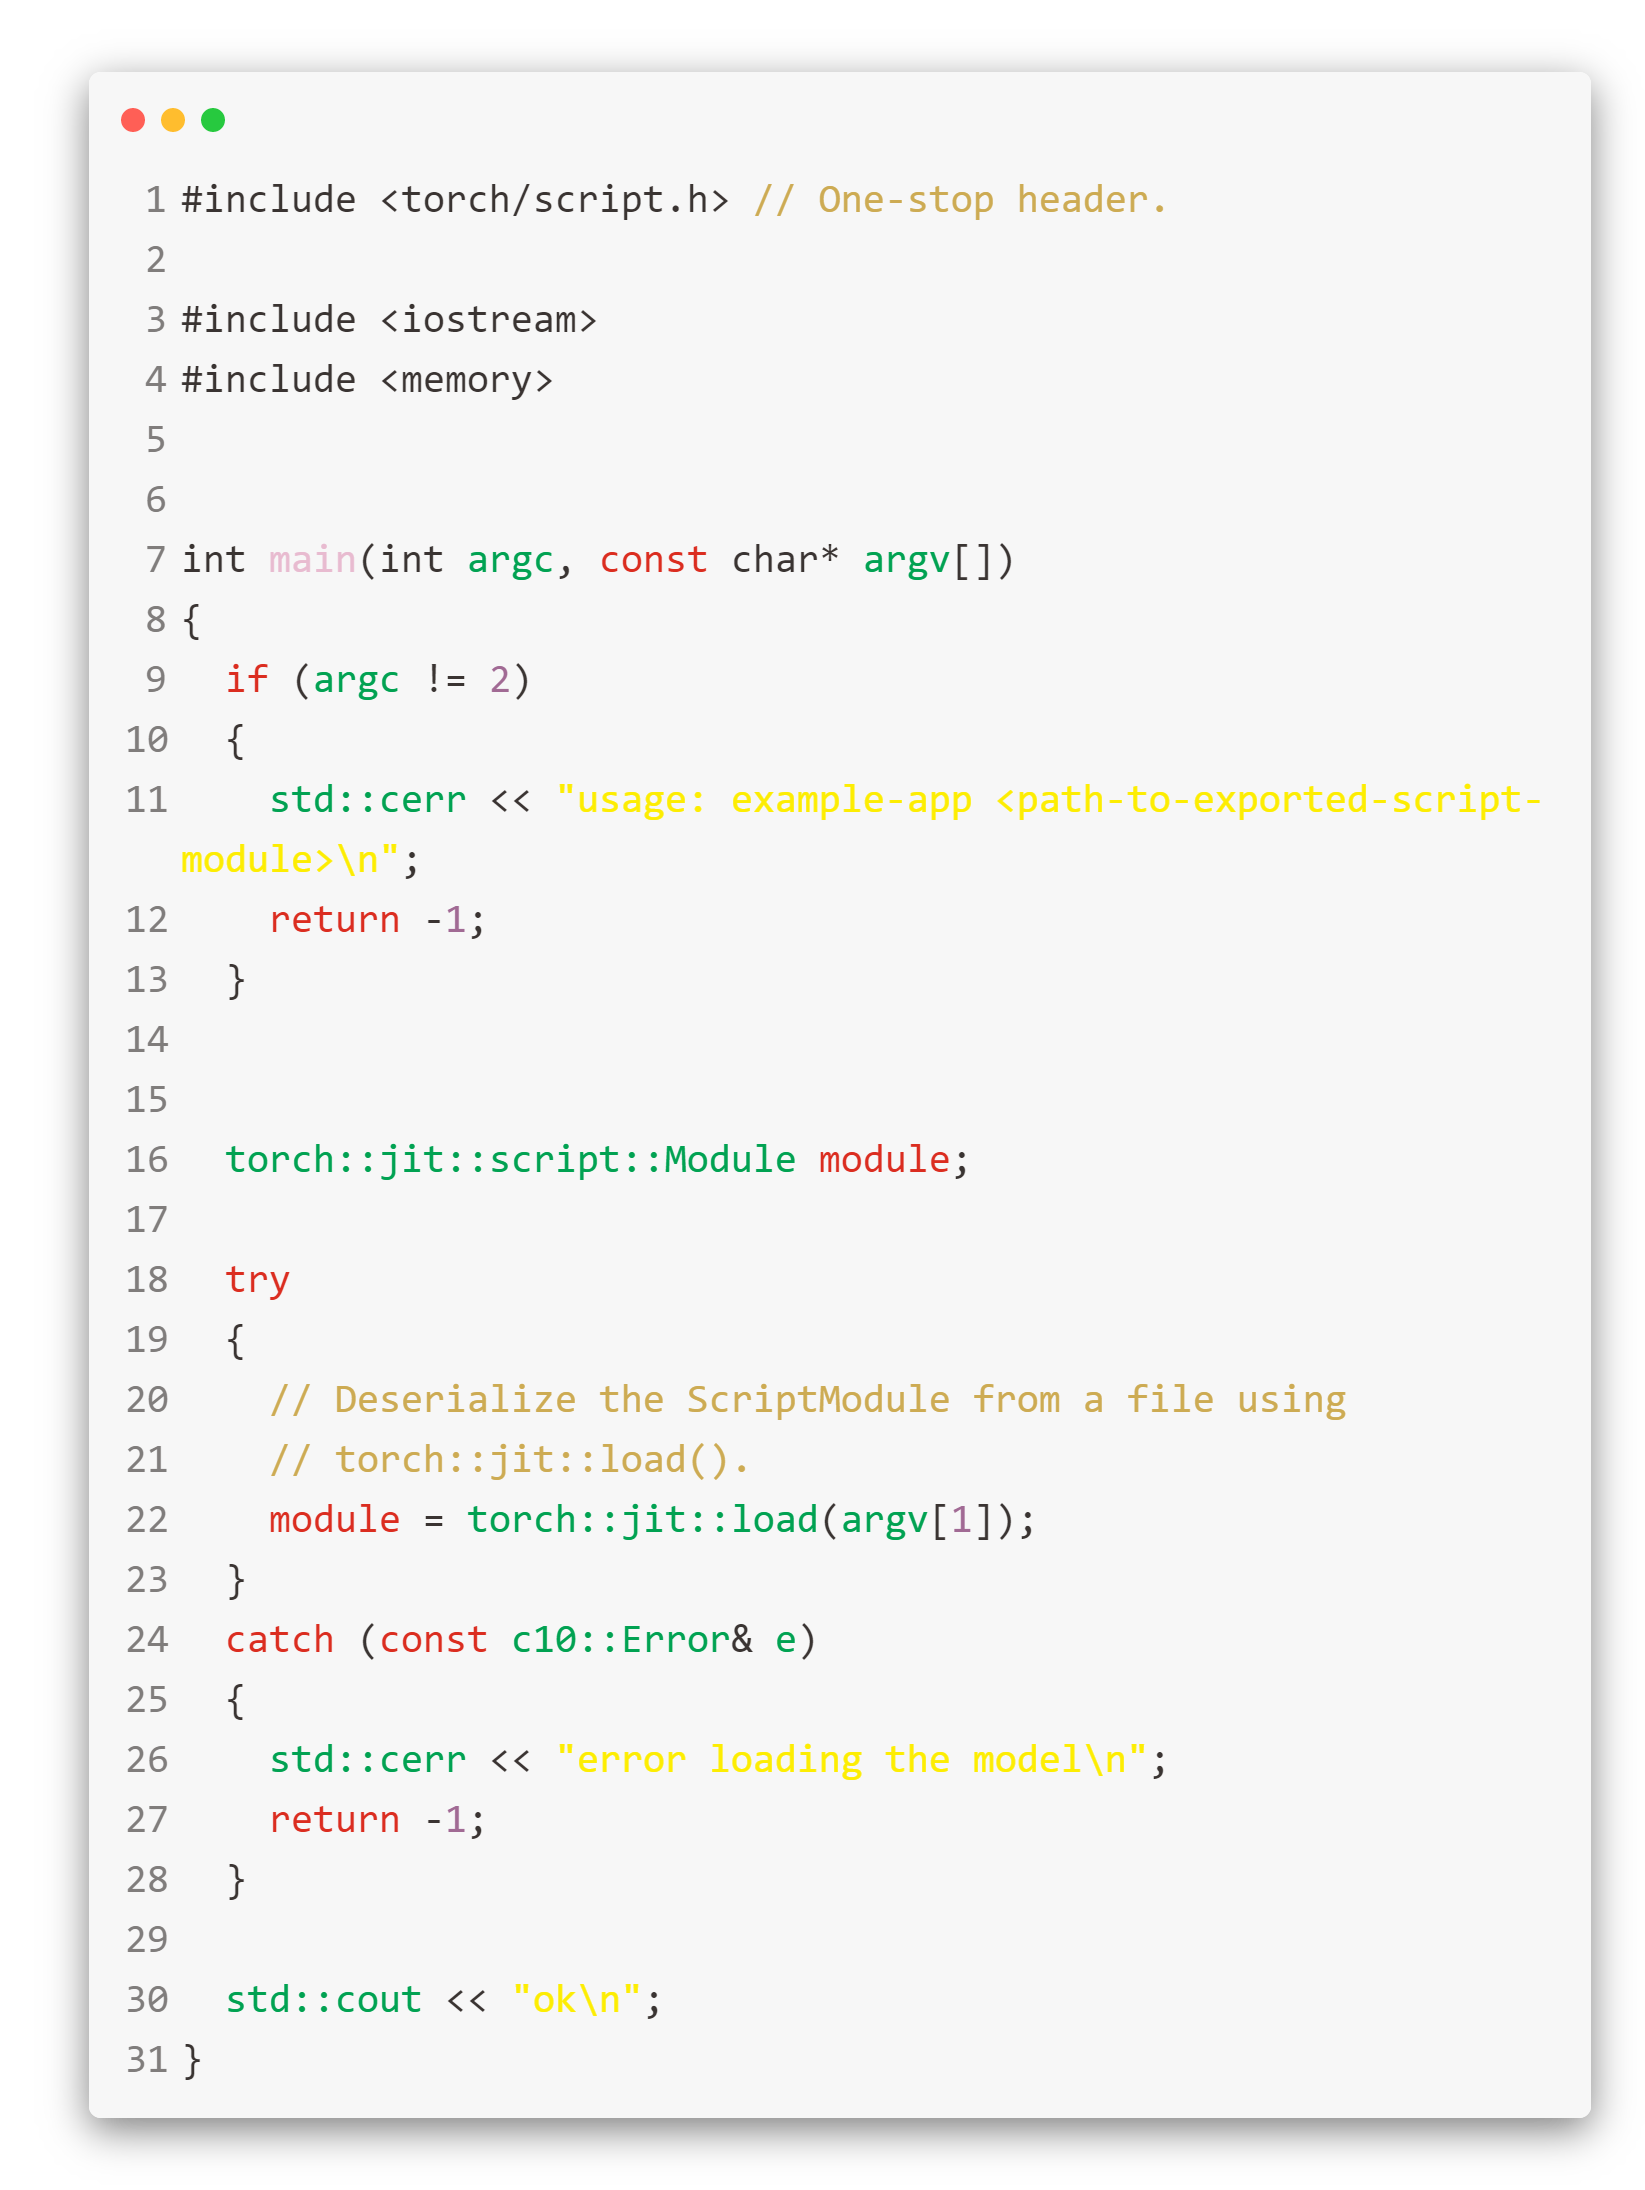
\includegraphics[width=0.98\linewidth]{figures/code-cpp-big.png}
%    \caption{Pytorch 模型在 C++ 项目中的应用}
%    \label{fig:code_cpp}
%\end{figure}

\pagebreak
\section{系统的部署与展示}\label{figures_tables}

介绍本文系统的部署与测试。本文的系统是运行于 Windows 平台,具体的运行环境见表~\ref{tab:env2}。在运行系统之前需要编译和配置好相关运行库,比如 LibTorch、OpenCV、MYNTAI S1040-IR-120/Mono的 SDK。

\subsection{系统运行环境}
本系统的开发和运行环境如表~\ref{tab:env1} 和表~\ref{tab:env2} 所示,包含软件环境和硬件环境。图~\ref{fig:photo} 展示的是本系统的真实硬件环境以及相应的系统交互界面。
\begin{table}[thbp]
	\centering
	\small\def\arraystretch{2.5}\setlength\tabcolsep{0.08\textwidth}
	\caption{系统开发环境}
	\begin{tabular}{|c|c|}
		\hline
		\multicolumn{2}{|c|}{软件环境}                \\
		\hline
		操作系统   & Ubuntu 18.04 \\
		\hline
		开发语言   & python、C++、matlab \\
		\hline
		运行环境  & python 3.6    \\
		\hline
		\multicolumn{2}{|c|}{硬件环境} \\
		\hline
		处理器    &      Intel(R) Core(TM) i5-4210U CPU @ 2.50 GHz  \\
		\hline
		内存      &       8GB         \\
		\hline
		显卡    &     TITAN X       \\
		\hline
	\end{tabular}
	\label{tab:env1}
\end{table}

\begin{table}[thbp]
	\centering
	\small\def\arraystretch{2.}\setlength\tabcolsep{0.05\textwidth}
	\caption{系统运行环境}
	\begin{tabular}{|c|c|}
		\hline
		\multicolumn{2}{|c|}{软件环境}                \\
		\hline
		操作系统   & Windows 10 					  \\
		\hline
		开发工具  & Matlab 2018b  					   \\
		\hline
		运行库   & LibTorch、OpenCV、MYNTAI S1040-IR-120/Mono SDK \\
		\hline
		\multicolumn{2}{|c|}{硬件环境} \\
		\hline
		处理器    &      Intel(R) Core(TM) i5-4210U CPU @ 2.50 GHz  \\
		\hline
		内存      &       8GB         \\
		\hline
		传感器    &     MYNTAI S1040-IR-120/Mono          \\
		\hline
	\end{tabular}
	\label{tab:env2}
\end{table}

\begin{figure}[htbp]
	\centering
	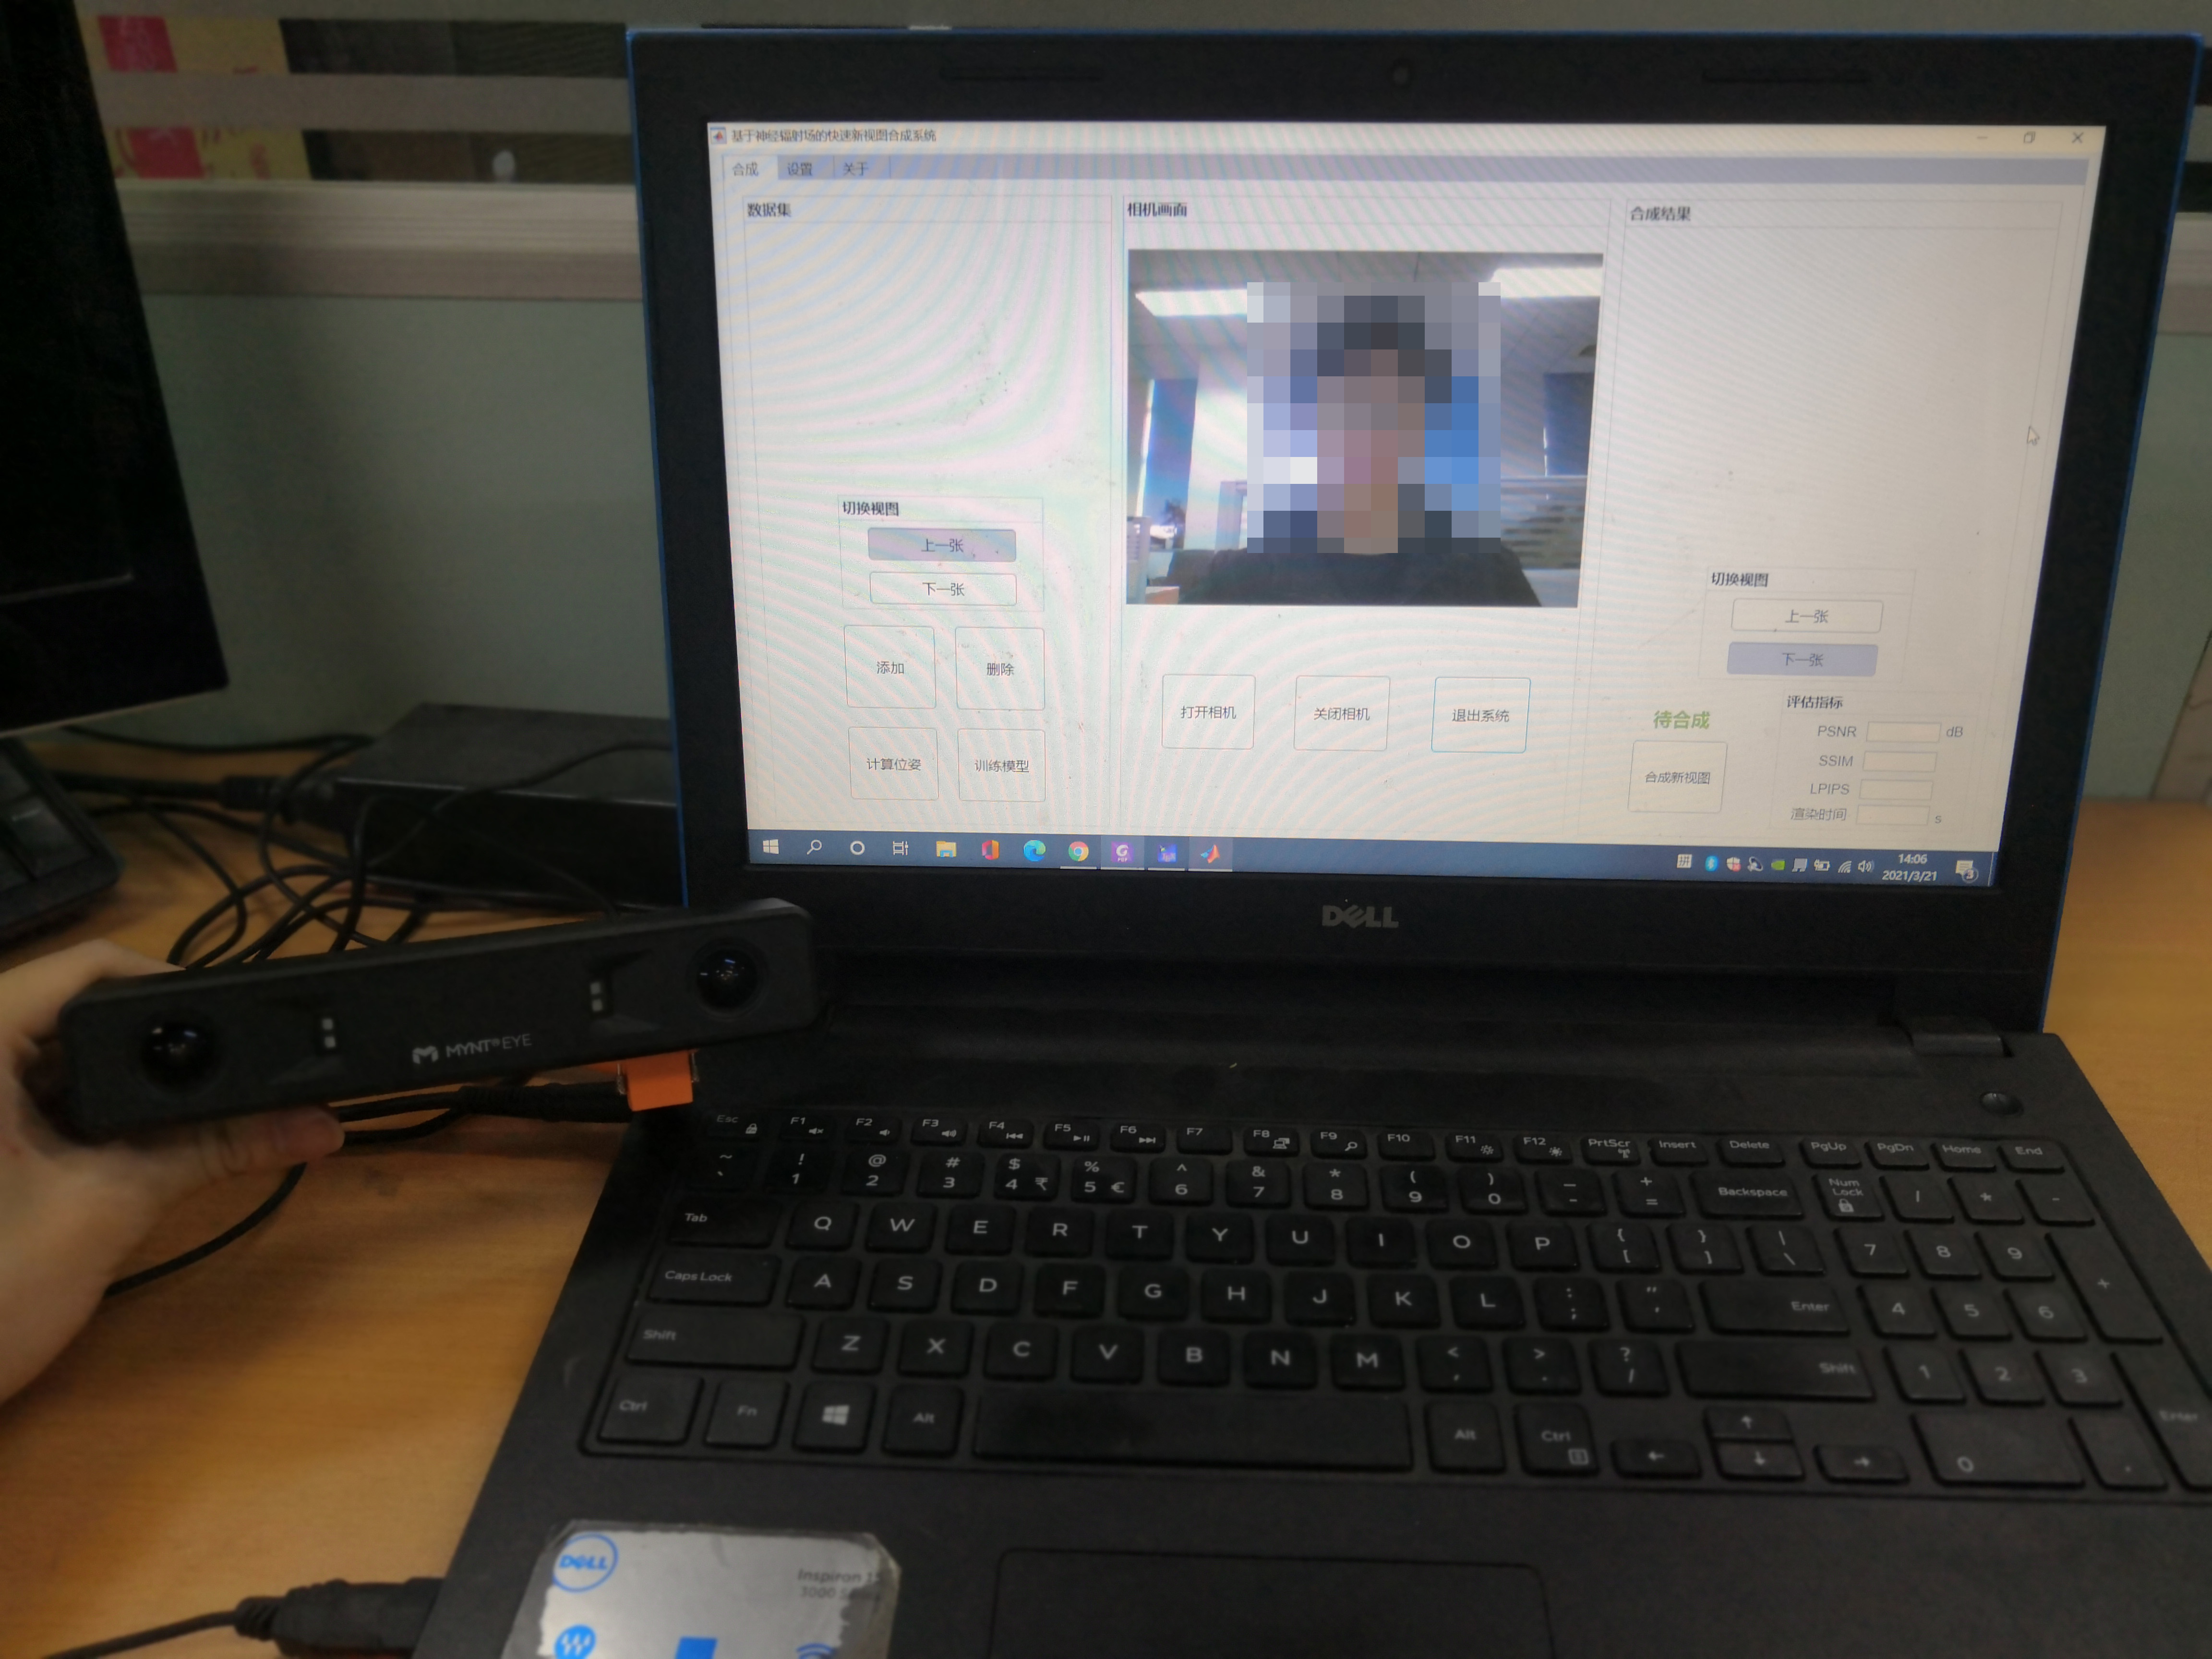
\includegraphics[width=0.85\linewidth]{figures/system-hardware.jpg}
	\caption{系统的硬件环境}
	\label{fig:photo}
\end{figure}
\pagebreak
\subsection{系统功能测试}
本小节针对本系统的各个模块进行测试,下面将详述测试的过程,并展示与用户交互的界面以及最终测试的结果。
\subsubsection{相机交互功能测试}
首先我们先测试电脑与相机方面的交互功能。与相机能够友好交互,获得稳定高质量的图像,这对整个训练或者测试都是意义重大地。相机传感器是数据的本源,是一切计算机视觉的基础和灵魂。拥有着一个鲁棒而友好的相机交互环境能为新视图合成任务提供非常好的输入,容易让网络学习到更准确的神经辐射场,预测出更准的颜色和体密度,这些都会在 PSNR、SSIM、LPIPS等指标上面体现出来。

\begin{table}[thbp]
	\centering
	\small\def\arraystretch{1.5}\setlength\tabcolsep{0.05\textwidth}
	\caption{相机交互功能测试用例}
	\begin{tabular}{|p{2cm}<{\centering}|p{4cm}<{\centering}|p{4cm}<{\centering}|}
		\hline
		用例编号 & \multicolumn{2}{|l|}{001}       \\
		\hline
		测试功能 & \multicolumn{2}{|l|}{相机交互}       \\
		\hline
		编号 & 输入/动作 & 期望结果 \\
		\hline
		1 & 打开应用,进入合成界面,在相机画面栏点击打开相机按钮 & 跳转到传感器 RGBD 相机界面 \\
		\hline
		2 & 在数据集栏点击添加按钮 & 当前相机的图像被捕获到数据集栏 \\
		\hline
		3 & 在相机画面栏点击关闭相机 & 提示:“您确定要关闭相机吗?” \\
		\hline
		4 & 点击确认关闭 & 相机画面终止 \\
		\hline
		5 & 点击取消关闭 & 整个交互界面不变 \\
		\hline
		6 & 点击退出系统 & 提示:“您确定退出吗?” \\
		\hline
		7 & 点击确认退出 & 整个交互界面退出 \\
		\hline
		8 & 点击取消退出 & 整个交互界面不变 \\
		\hline
	\end{tabular}
	\label{tab:camera}
\end{table}
根据表~\ref{tab:camera},整个数据集处理的测试步骤如下:
\begin{enumerate}
	\item[1)] 打开应用进入合成菜单栏,点击打开相机按钮,测试结果如图~\ref{fig:camara-a} 和图~\ref{fig:camara-b}。用例001编号为1的测试符合预期结果。
	\item[2)] 在数据集面板上点击添加,当前相机画面会被捕获到数据集,具体测试如图~\ref{fig:camara-c}。用例001编号为2的测试符合预期结果。
	\item[3)] 若点击了相机界面的关闭相机按钮,会有相应提示信息,如图~\ref{fig:camara-d} 所示。若点击是,则相机画面终止,如图~\ref{fig:camara-e} 所示。若点击否,则保持不变,如图~\ref{fig:camara-c}。用例001编号为3、4、5的测试符合预期结果。
	\item[4)] 若点击了相机界面的退出系统按钮,会有相应提示信息,如图~\ref{fig:camara-f} 所示。若点击是,则程序画面终止。若点击否,则保持不变,如图~\ref{fig:camara-e}。用例001编号为6、7、8的测试符合预期结果。
\end{enumerate}

\begin{figure}[bhtp]
	\centering
	\subcaptionbox{打开应用画面\label{fig:camara-a}}
	{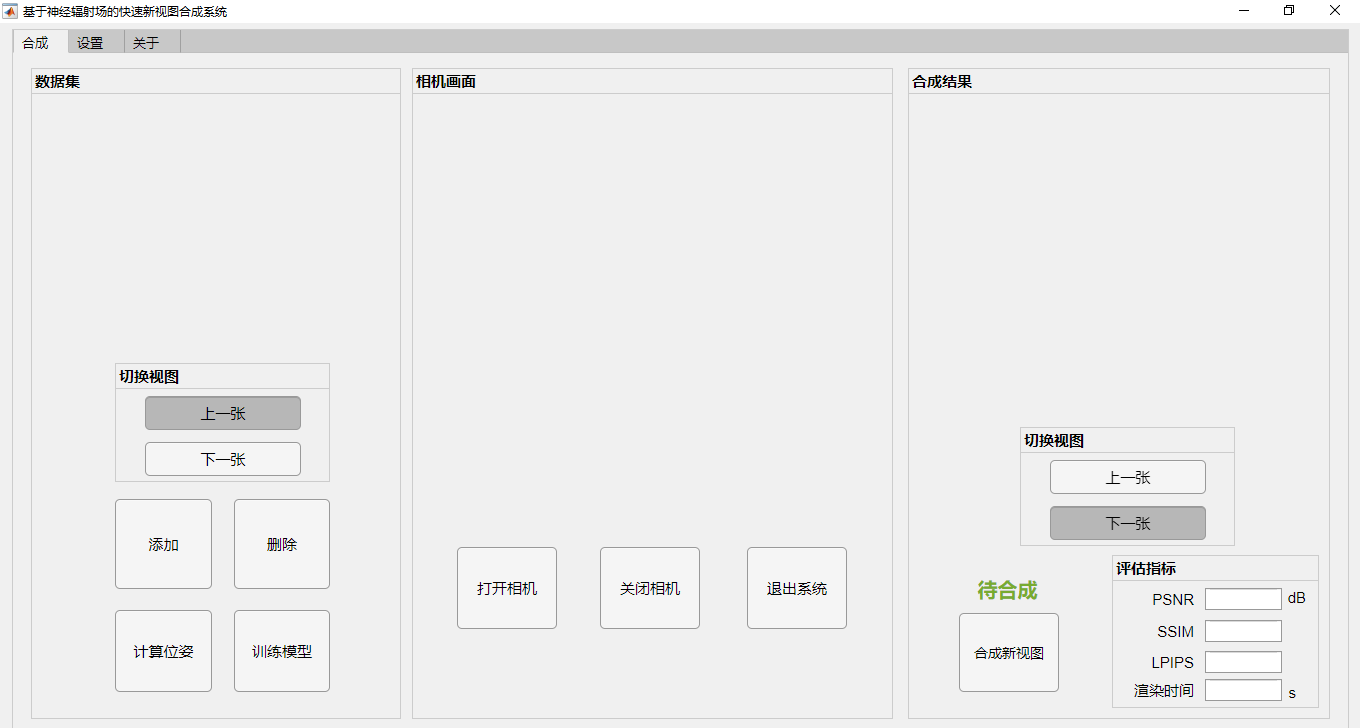
\includegraphics[width=0.45\linewidth]{figures/system/1-a.png}}
	\subcaptionbox{打开相机画面\label{fig:camara-b}}
	{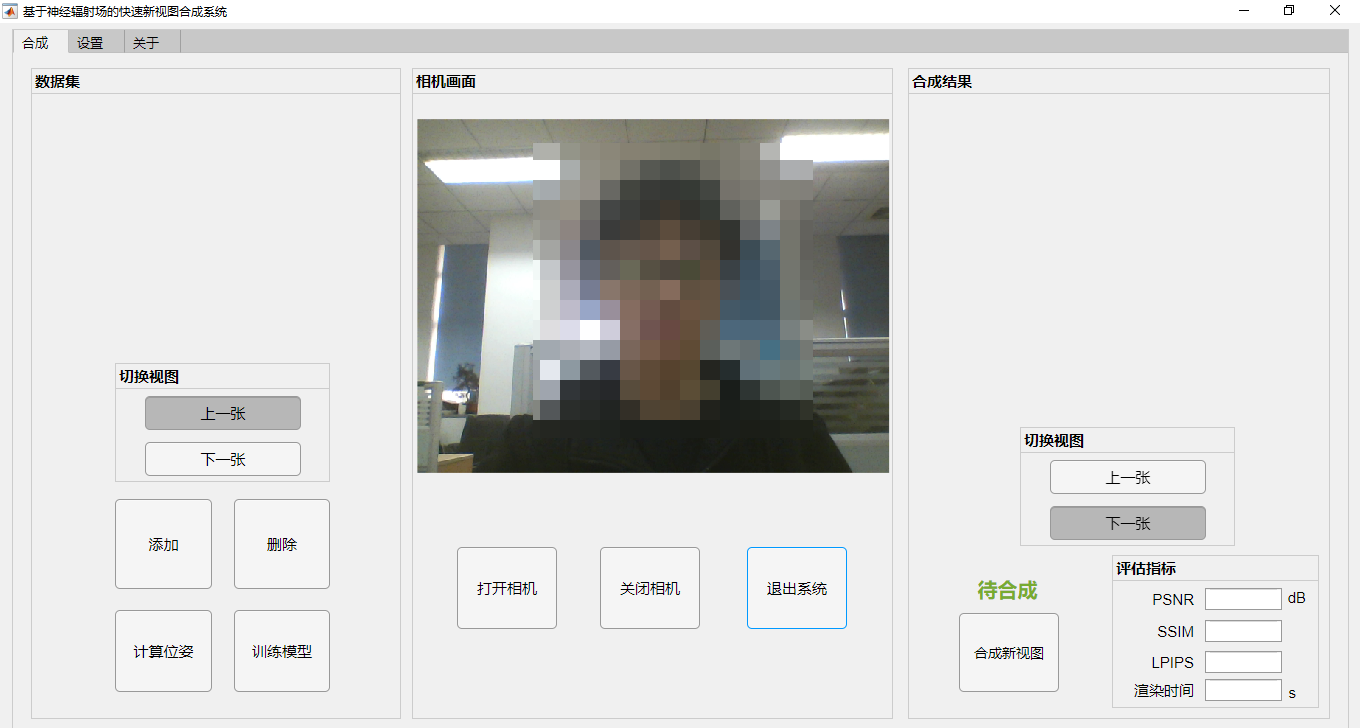
\includegraphics[width=0.45\linewidth]{figures/system/1-b.png}} \\
	\subcaptionbox{捕获相机画面\label{fig:camara-c}}
	{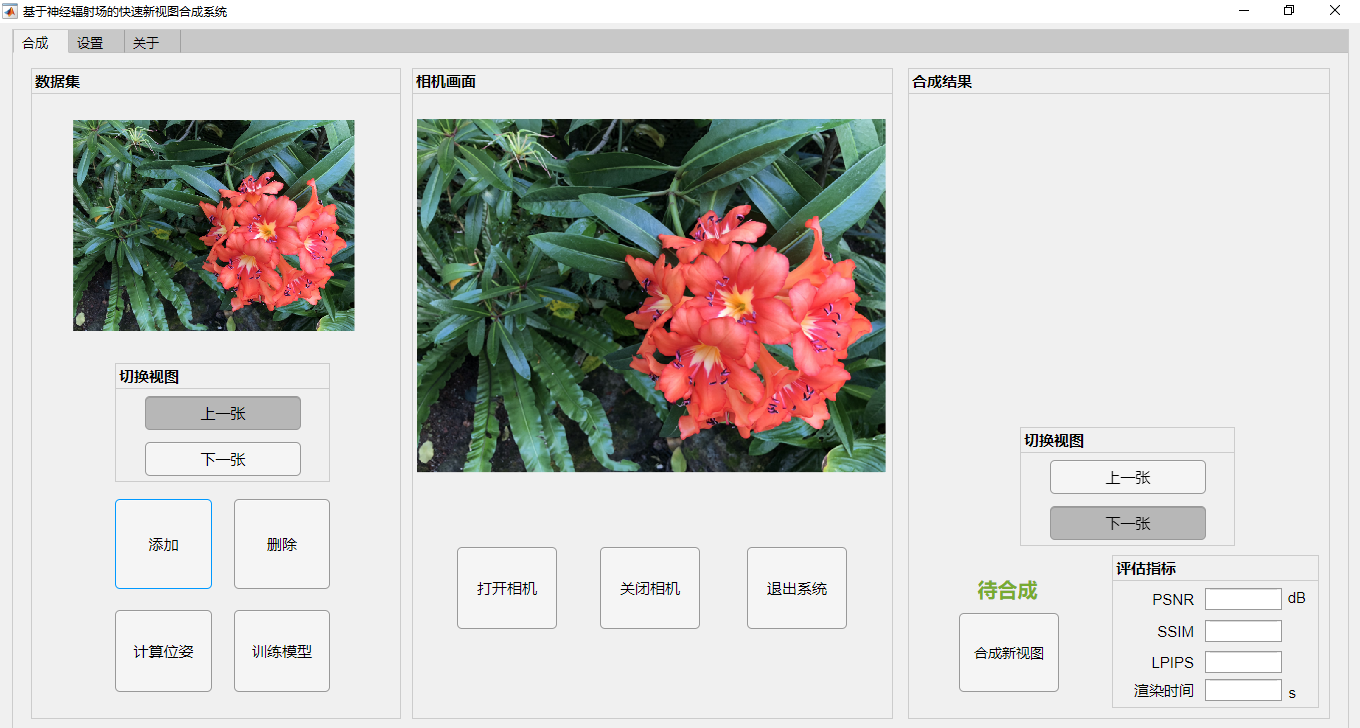
\includegraphics[width=0.45\linewidth]{figures/system/1-c.png}}
	\subcaptionbox{关闭相机提示信息\label{fig:camara-d}}
	{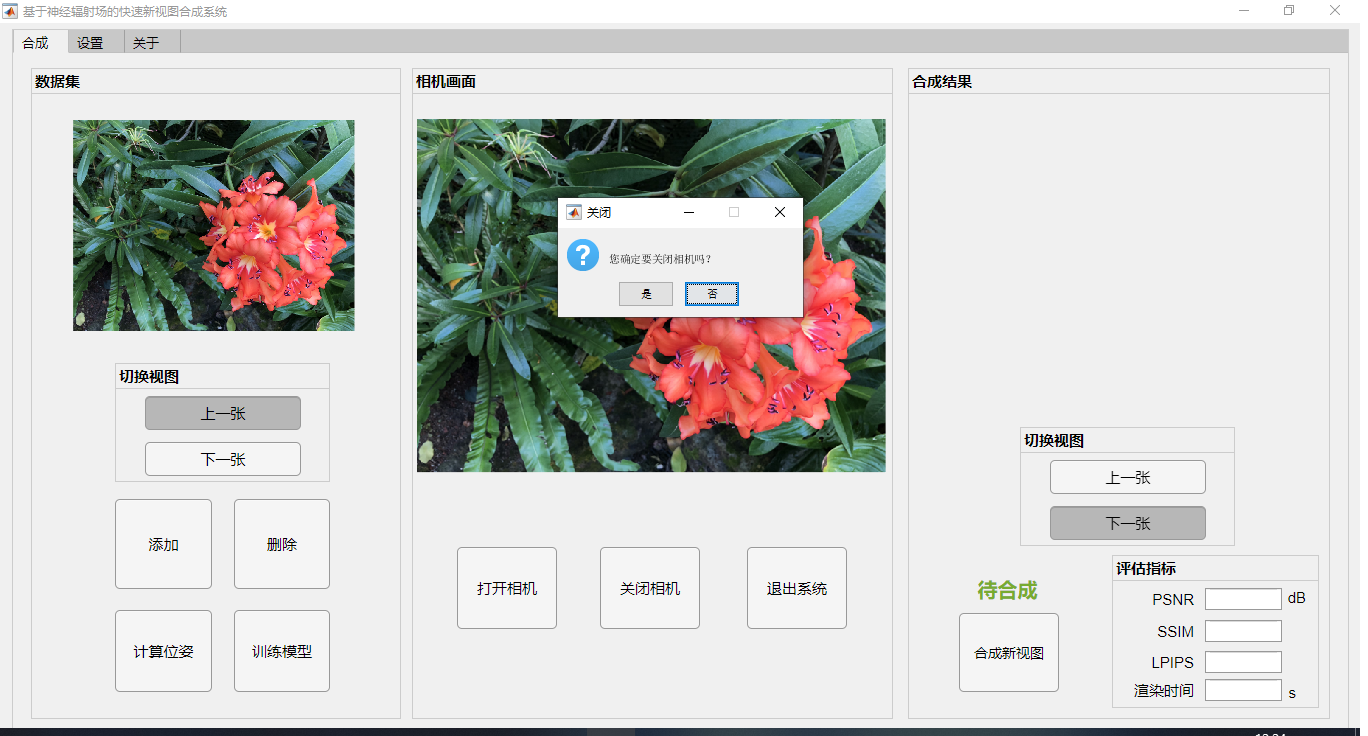
\includegraphics[width=0.45\linewidth]{figures/system/1-d.png}} \\
	\subcaptionbox{关闭相机画面\label{fig:camara-e}}
	{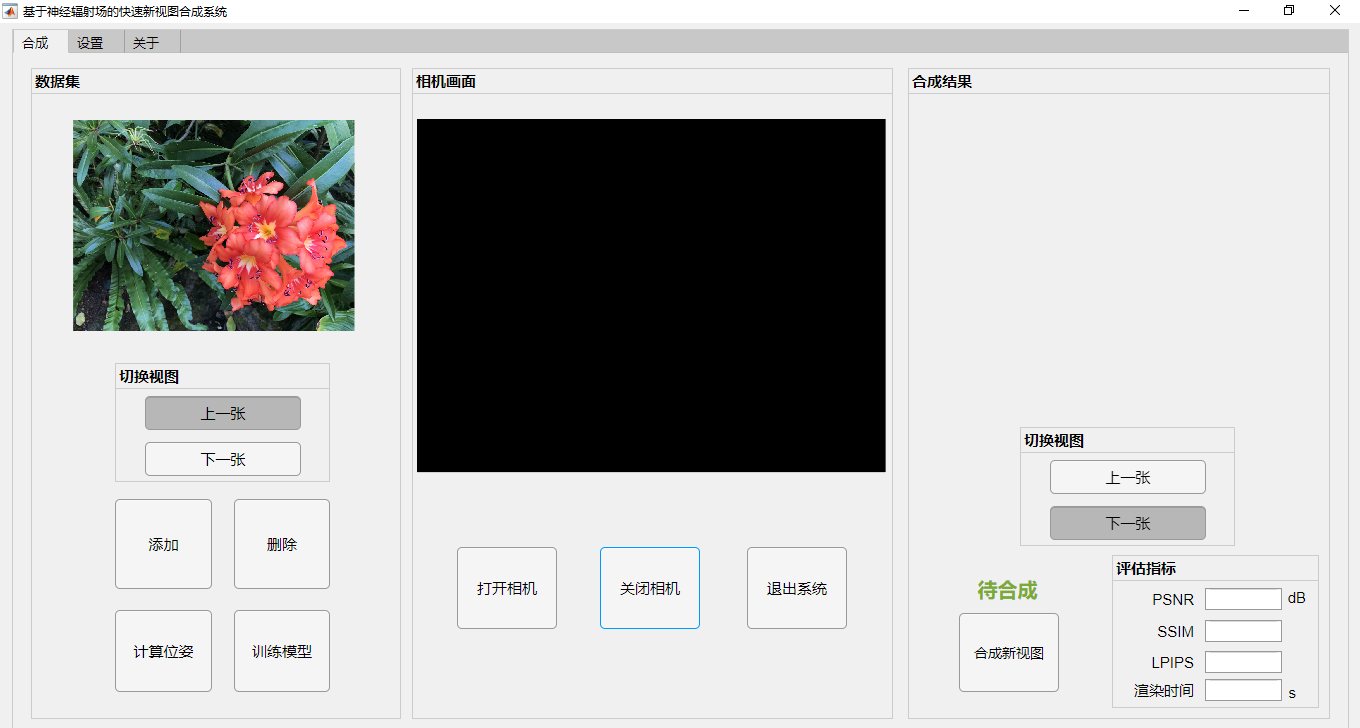
\includegraphics[width=0.45\linewidth]{figures/system/1-e.png}}
	\subcaptionbox{退出应用提示信息\label{fig:camara-f}}
	{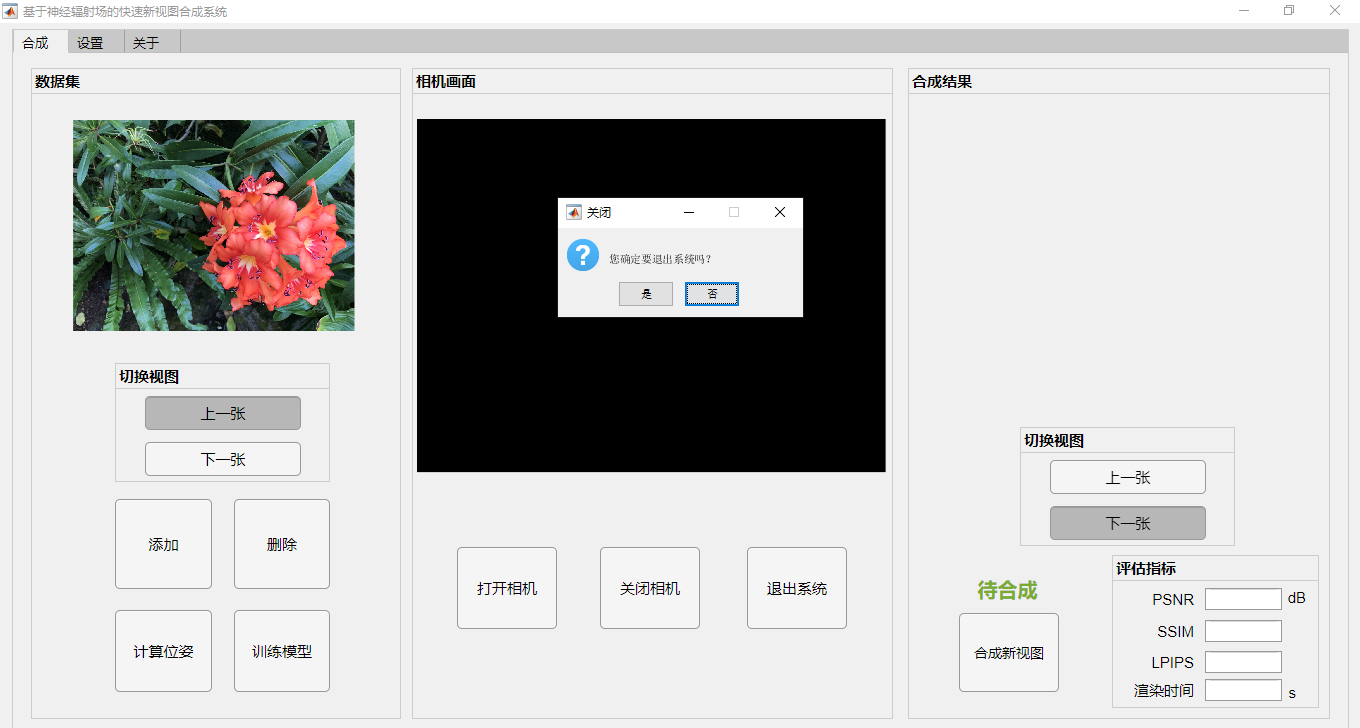
\includegraphics[width=0.45\linewidth]{figures/system/1-f.png}}
	\caption{相机交互功能测试}
	\label{fig:camara}
\end{figure}
\newpage

\subsubsection{数据集处理功能测试}
数据集处理是整个系统的最先使用的功能,非常至关重要,数据的选取决定了最终测试结果的好坏。数据集处理对应于本系统数据处理模块的功能。首先介绍下数据处理模块对应的典型测试用例,主要包含数据集的获取,删除。

\begin{table}[t]
	\centering
	\small\def\arraystretch{1.3}\setlength\tabcolsep{0.05\textwidth}
	\caption{数据集处理功能测试用例}
	\begin{tabular}{|p{2cm}<{\centering}|p{4cm}<{\centering}|p{4cm}<{\centering}|}
		\hline
		用例编号 & \multicolumn{2}{|l|}{002}       \\
		\hline
		测试功能 & \multicolumn{2}{|l|}{数据集处理}       \\
		\hline
		编号 & 输入/动作 & 期望结果 \\
		\hline
		1 & 打开应用,进入合成界面,在相机画面栏点击打开相机按钮 & 跳转到传感器 RGBD 相机界面 \\
		\hline
		2 & 在数据集栏点击添加按钮 & 当前相机的 RGB 数据被选作数据集并显示在数据集栏上 \\
		\hline
		3 & 在数据集栏点击上(下)一张按钮 & 数据集栏画面切换为上(下)一张图像 \\
		\hline
		4 & 在数据集栏点击删除按钮 & 提示:“您确定删除吗?” \\
		\hline
		5 & 点击确认删除 & 数据集栏当前显示的图像被删除 \\
		\hline
		6 & 点击取消删除或者提示栏右上角$\times$ & 数据集栏当前显示的图像被保留在数据集中 \\
		\hline
	\end{tabular}
	\label{tab:getdataset}
\end{table}

根据表~\ref{tab:getdataset},整个数据集处理的测试步骤如下:
\begin{enumerate}
	\item[1)] 打开应用进入合成菜单栏,点击打开相机按钮,测试结果如图~\ref{fig:camara-b}。用例002编号为1的测试与预期结果相符。
	\item[2)] 在数据集面板上点击添加,当前相机画面会被捕获到数据集,如图~\ref{fig:camara-c}。用例002编号为2的测试符合预期结果。
	\item[3)] 若点击数据集栏上(下)一张按钮,视图会切换到上(下)一张图像,如图~\ref{fig:datasetProcess-a} 和图~\ref{fig:datasetProcess-b}。用例002编号为3的测试符合预期结果。
	\item[4)] 若在数据集栏点击了删除按钮,会有相应提示信息,如图~\ref{fig:datasetProcess-c}。若点击是,则数据集当前画面终止,如图~\ref{fig:datasetProcess-d} 所示。若点击否,则保持不变,如图~\ref{fig:camara-e}。用例002编号为4、5、6的测试符合预期结果。
\end{enumerate}
\pagebreak
\begin{figure}[thbp]
	\centering 
	% 0.55
	\subcaptionbox{上一张捕获图像\label{fig:datasetProcess-a}}
	{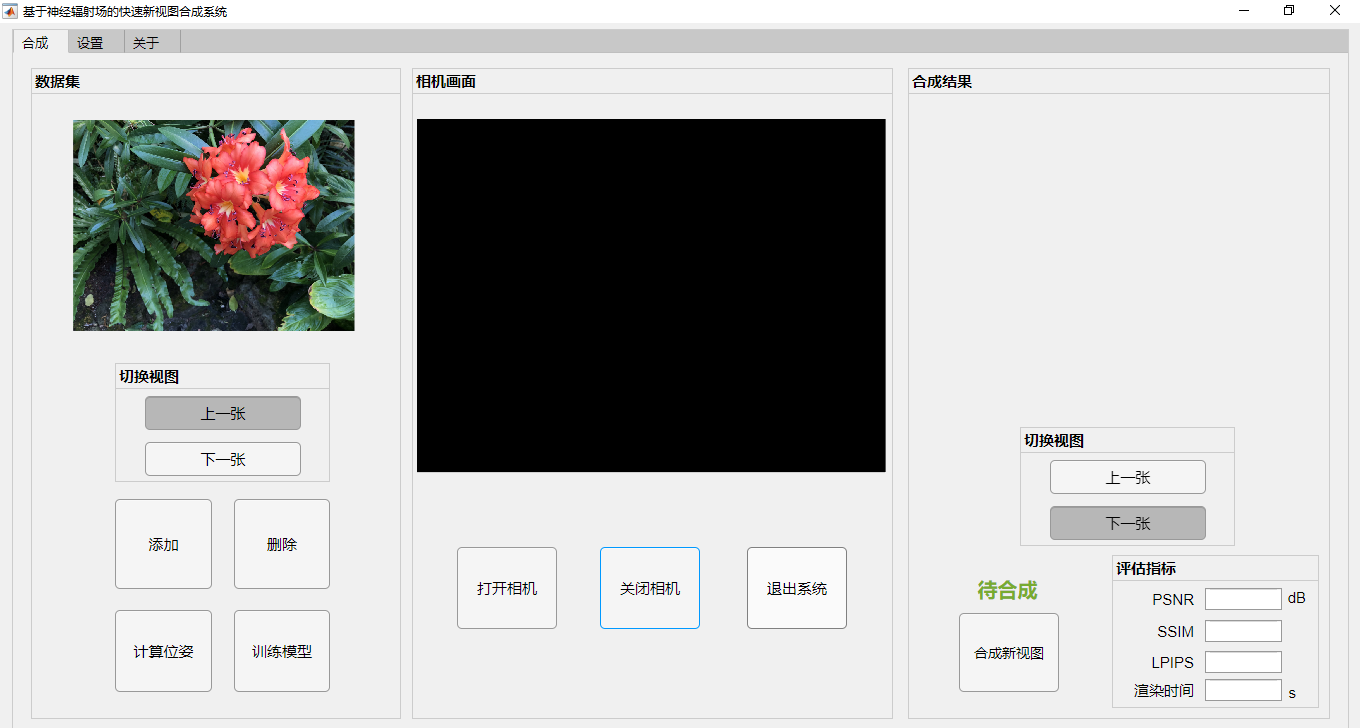
\includegraphics[width=0.45\linewidth]{figures/system/2-a.png}}
	\subcaptionbox{下一张捕获图像\label{fig:datasetProcess-b}}
	{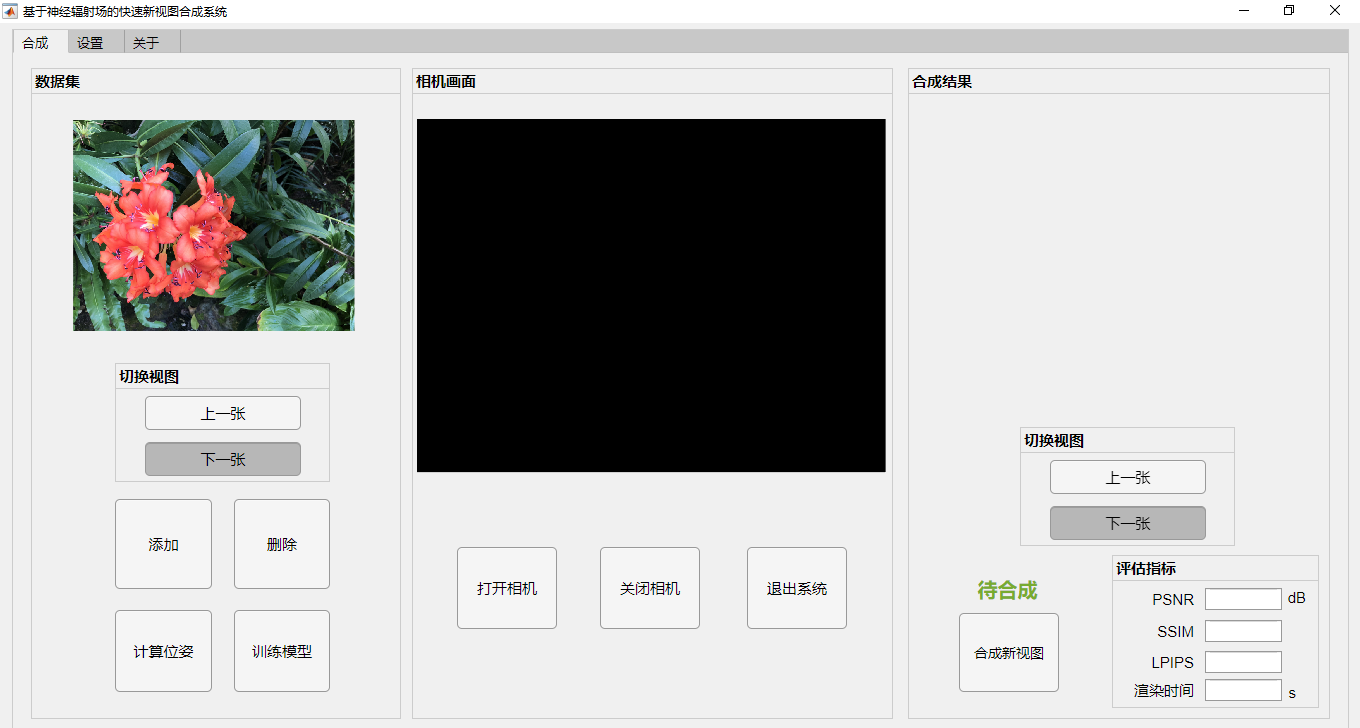
\includegraphics[width=0.45\linewidth]{figures/system/2-b.png}}
	\subcaptionbox{删除数据的提示信息\label{fig:datasetProcess-c}}
	{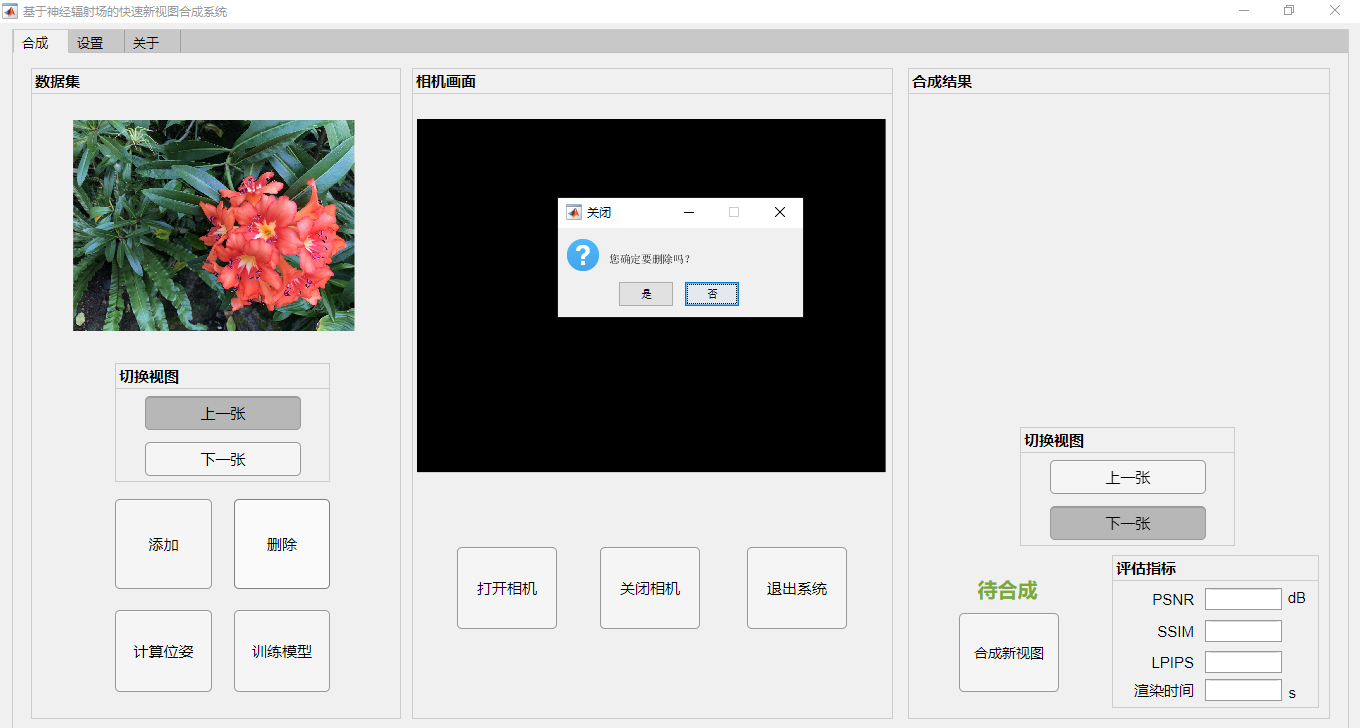
\includegraphics[width=0.45\linewidth]{figures/system/2-c.png}}
	\subcaptionbox{删除后的画面\label{fig:datasetProcess-d}}
	{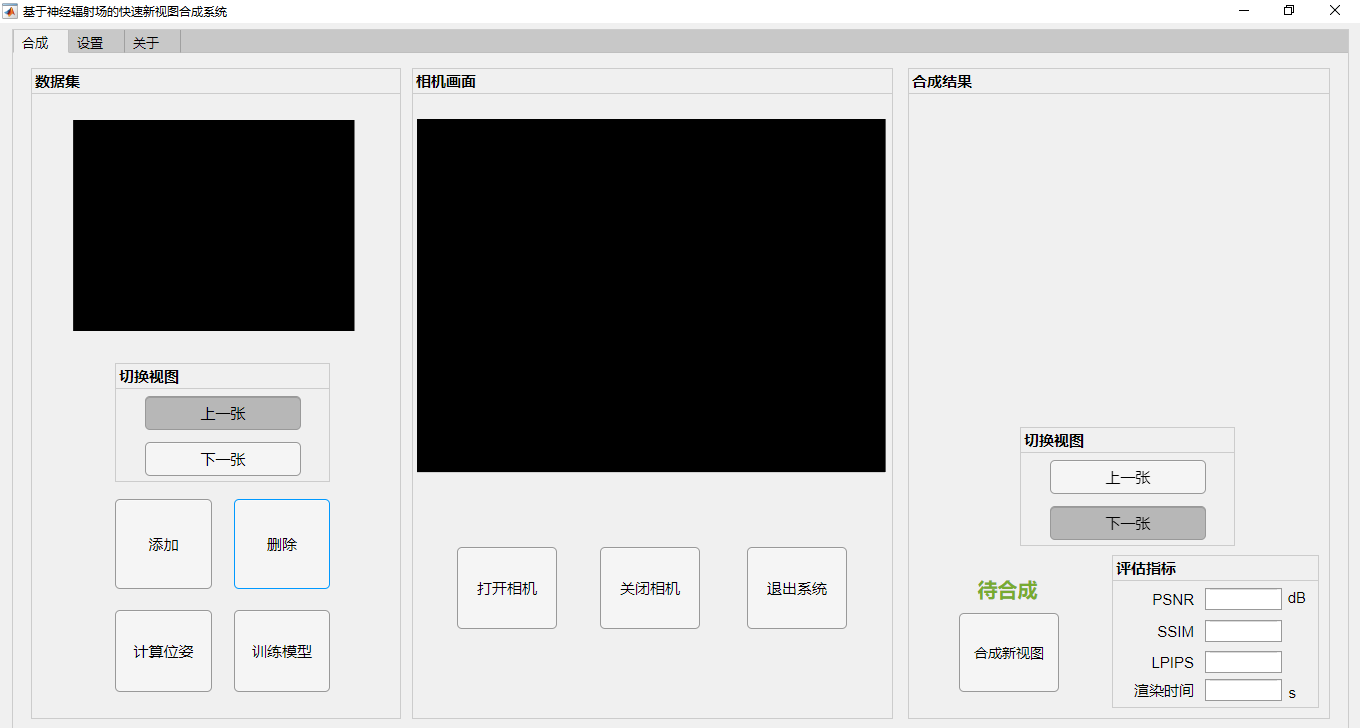
\includegraphics[width=0.45\linewidth]{figures/system/2-d.png}}
	\caption{数据集处理功能测试}
	\label{fig:datasetProcess}
\end{figure}

\begin{table}[htbp]
	\centering
	\small\def\arraystretch{0.9}\setlength\tabcolsep{0.05\textwidth}
	\caption{新视图合成功能测试用例}
	\begin{tabular}{|p{2cm}<{\centering}|p{4cm}<{\centering}|p{4cm}<{\centering}|}
		\hline
		用例编号 & \multicolumn{2}{|l|}{003}       \\
		\hline
		测试功能 & \multicolumn{2}{|l|}{新视图合成}       \\
		\hline
		编号 & 输入/动作 & 期望结果 \\
		\hline
		1 & 点击计算位姿按钮 &  进度条提示计算位姿的过程 \\
		\hline
		2 & 点击训练模型按钮 &  进度条提示模型训练的过程 \\
		\hline
		3 & 点击合成新视图按钮 & 状态提示从待合成到合成中再到已合成 \\
		\hline
		4 & 在合成栏点击上(下)一张按钮 & 数据集栏画面切换为上(下)一张图像,并显示相应的指标信息 \\
		\hline
	\end{tabular}
	\label{tab:viewsynthesis}
\end{table}
\subsubsection{新视图合成功能测试}
基于之前的功能测试,对于本系统的任务来说并不够,因为还没有检验本文方法的可行性与效率。基于神经辐射场的快速新视图合成,最终必须落脚于新视图合成,并对其进行加速。为了和之前保持一致,本系统在训练和测试环节都使用 $504 \times 378$ 的图像。下面是整个系统的最后一部分测试,是为了检测本文整个方法的性能,包含渲染速度以及渲染质量(包含PSNR、SSIM、LPIPS)等指标。通过多方面去表征本系统能有效地对 NeRF 进行加速,加速后的合成视图界面大图如图~\ref{fig:viewsynthesisBig} 所示。
%\begin{table}[htbp]
%	\centering
%	\small\def\arraystretch{1.}\setlength\tabcolsep{0.05\textwidth}
%	\caption{新视图合成功能测试用例}
%	\begin{tabular}{|p{2cm}<{\centering}|p{4cm}<{\centering}|p{4cm}<{\centering}|}
%		\hline
%		用例编号 & \multicolumn{2}{|l|}{003}       \\
%		\hline
%		测试功能 & \multicolumn{2}{|l|}{新视图合成}       \\
%		\hline
%		编号 & 输入/动作 & 期望结果 \\
%		\hline
%		1 & 点击计算位姿按钮 &  进度条提示计算位姿的过程 \\
%		\hline
%		2 & 点击训练模型按钮 &  进度条提示模型训练的过程 \\
%		\hline
%		3 & 点击合成新视图按钮 & 状态提示从待合成到合成中再到已合成 \\
%		\hline
%		4 & 在合成栏点击上(下)一张按钮 & 数据集栏画面切换为上(下)一张图像,并显示相应的指标信息 \\
%		\hline
%	\end{tabular}
%	\label{tab:viewsynthesis}
%\end{table}
根据表~\ref{tab:viewsynthesis},整个新视图功能测试的详细步骤如下:
\begin{enumerate}
	\item[1)] 若点击计算位姿按钮,会有相应提示信息,如图~\ref{fig:viewsynthesis-a} 和图~\ref{fig:viewsynthesis-b} 所示。用例003编号为1的测试与预期结果相符。
	\item[2)] 若点击训练模型按钮,会有相应提示信息,如图~\ref{fig:viewsynthesis-c} 和图~\ref{fig:viewsynthesis-d} 所示。用例003编号为2的测试与预期结果相符。
	\item[3)] 若点击合成新视图按钮,会有标签提示进度,如图~\ref{fig:viewsynthesis-e} 和图~\ref{fig:viewsynthesis-f} 以及图\ref{fig:viewsynthesis-g}。用例003编号为3的测试与预期结果相符。
	\item[4)] 若点击数据集栏上(下)一张按钮,视图会切换到上(下)一张图像,并且会显示本文 F-NeRF 合成新视角下图像的渲染质量信息和渲染时间信息,其中质量包含 PSNR、SSIM、LPIPS。如图~\ref{fig:viewsynthesis-h}(上)和图~\ref{fig:viewsynthesis-g}(下)所示,渲染时间分别为\SI{4.23}{s}和\SI{4.33}{s}。用例002编号为4的测试与预期结果相符。
\end{enumerate}



\begin{figure}[bhtp]
	\centering
	\subcaptionbox{提示信息,计算位姿中\label{fig:viewsynthesis-a}}
	{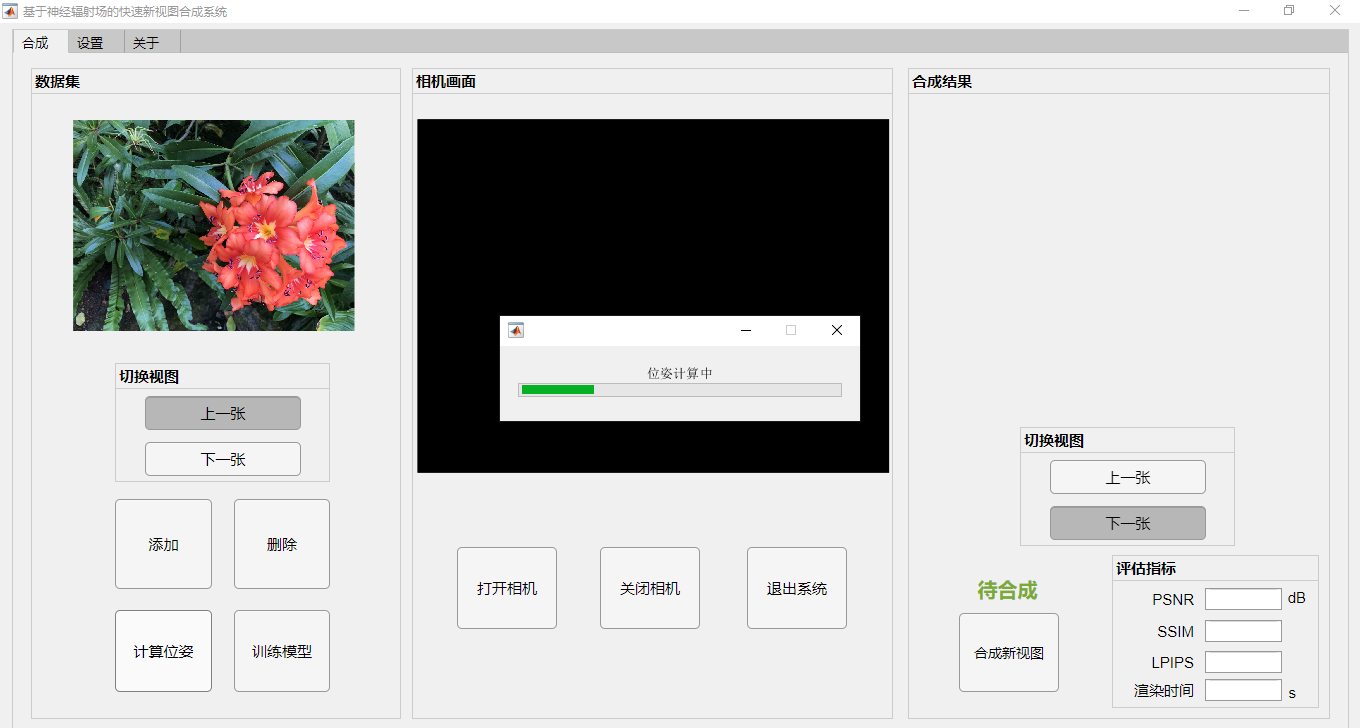
\includegraphics[width=0.45\linewidth]{figures/system/3-a.png}}
	\subcaptionbox{提示信息,计算位姿结束\label{fig:viewsynthesis-b}}
	{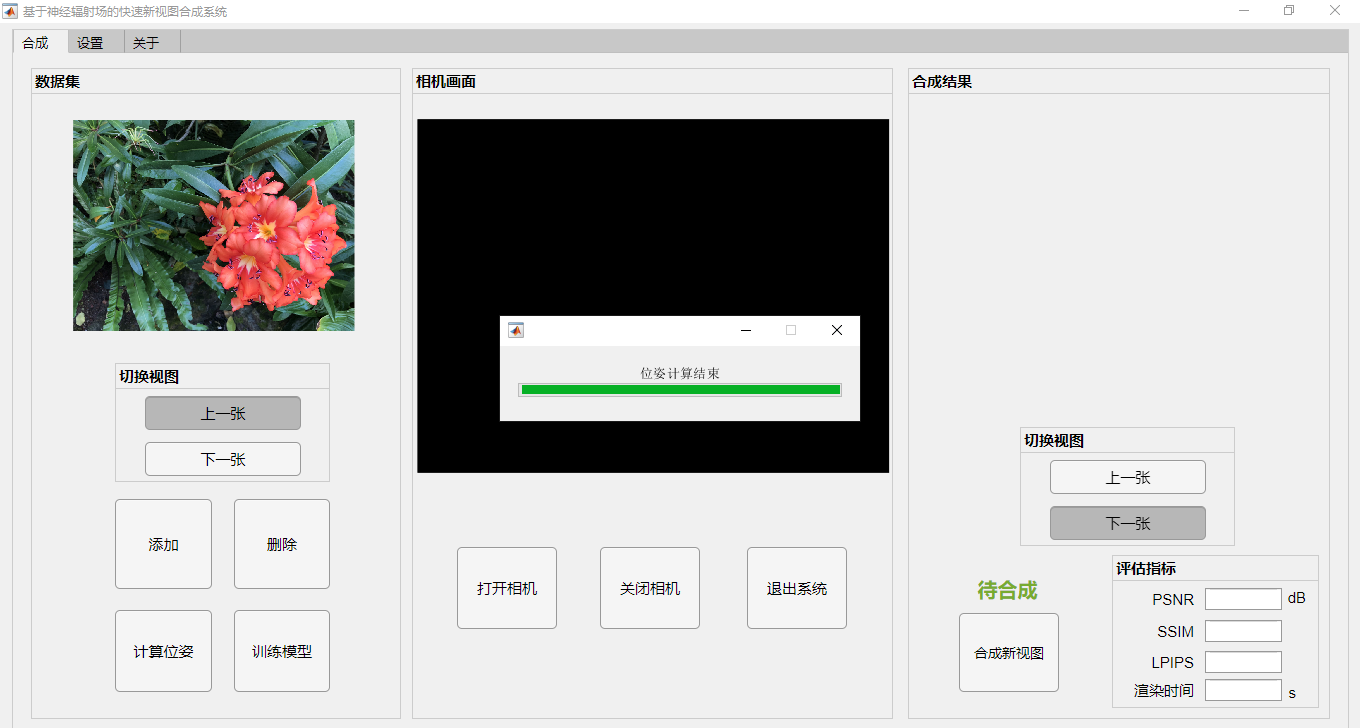
\includegraphics[width=0.45\linewidth]{figures/system/3-b.png}}
	\subcaptionbox{提示信息,训练中\label{fig:viewsynthesis-c}}
	{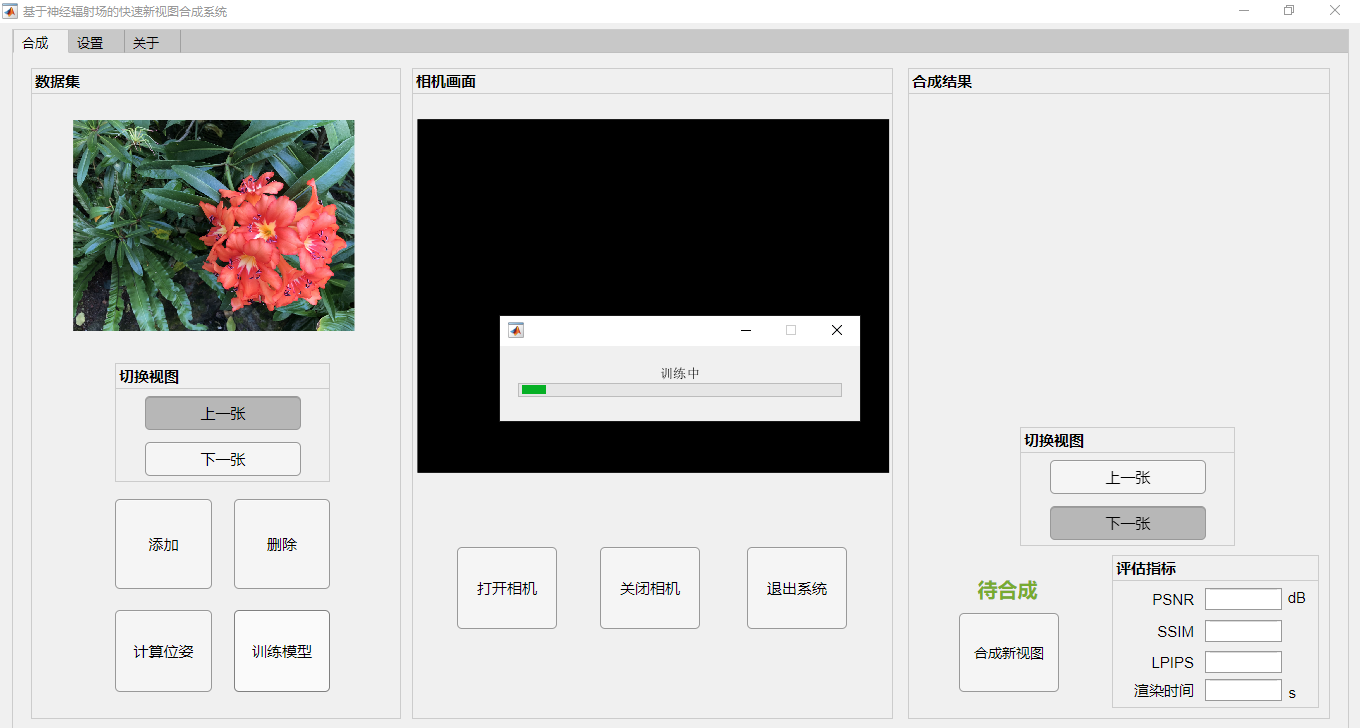
\includegraphics[width=0.45\linewidth]{figures/system/3-c.png}}
	\subcaptionbox{提示信息,训练结束\label{fig:viewsynthesis-d}}
	{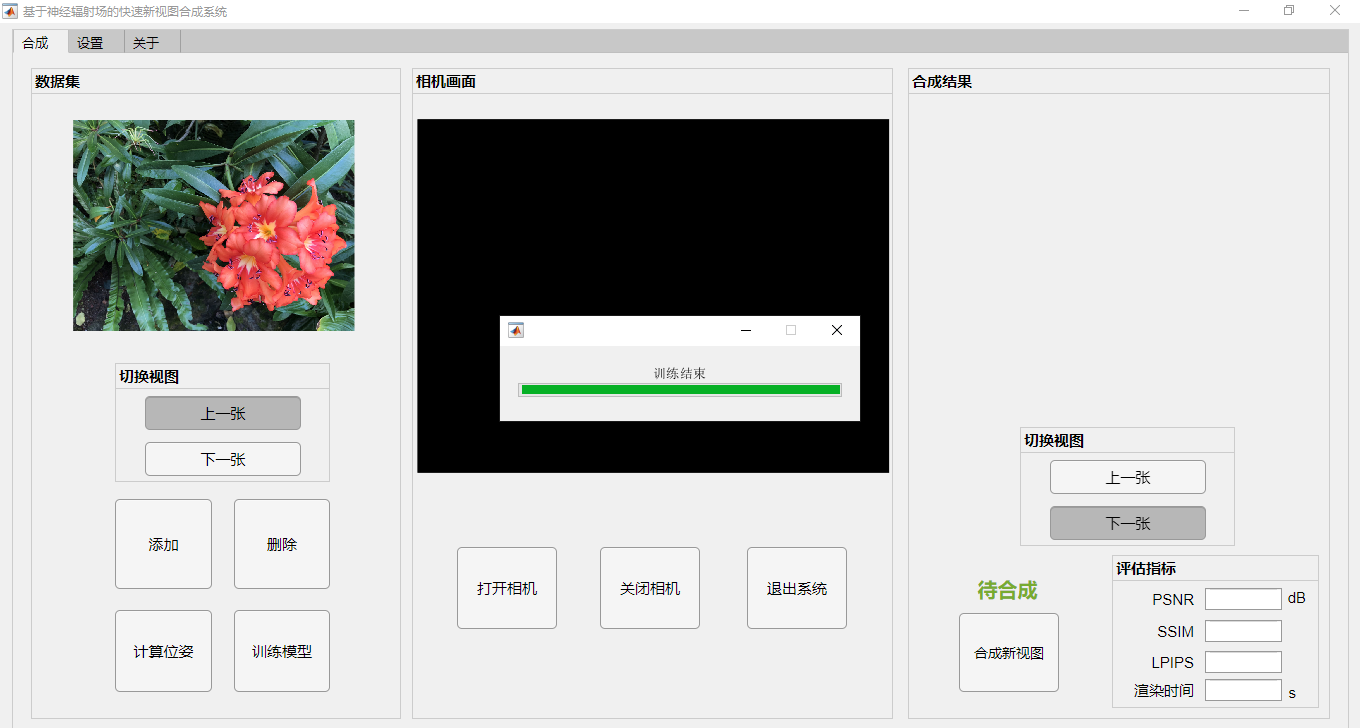
\includegraphics[width=0.45\linewidth]{figures/system/3-d.png}}
	\subcaptionbox{状态信息,待合成\label{fig:viewsynthesis-e}}
	{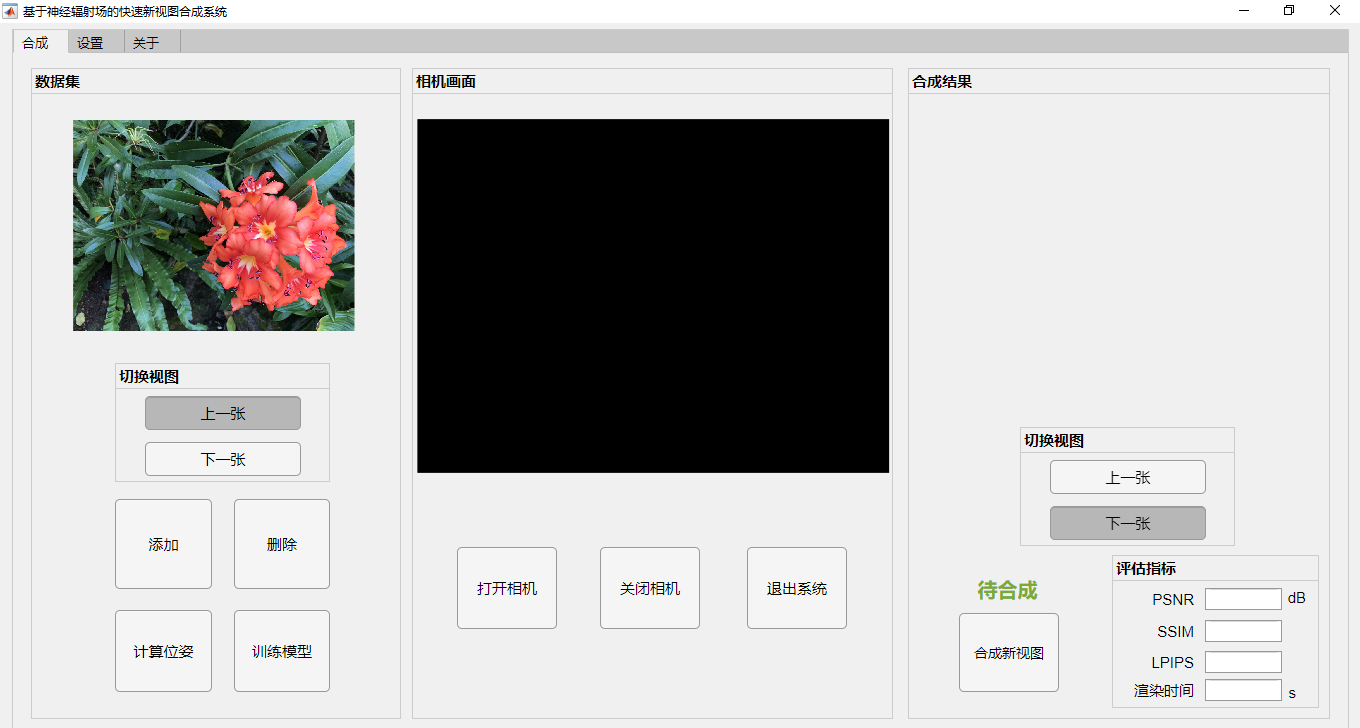
\includegraphics[width=0.45\linewidth]{figures/system/3-e.png}}
	\subcaptionbox{状态信息,合成中\label{fig:viewsynthesis-f}}
	{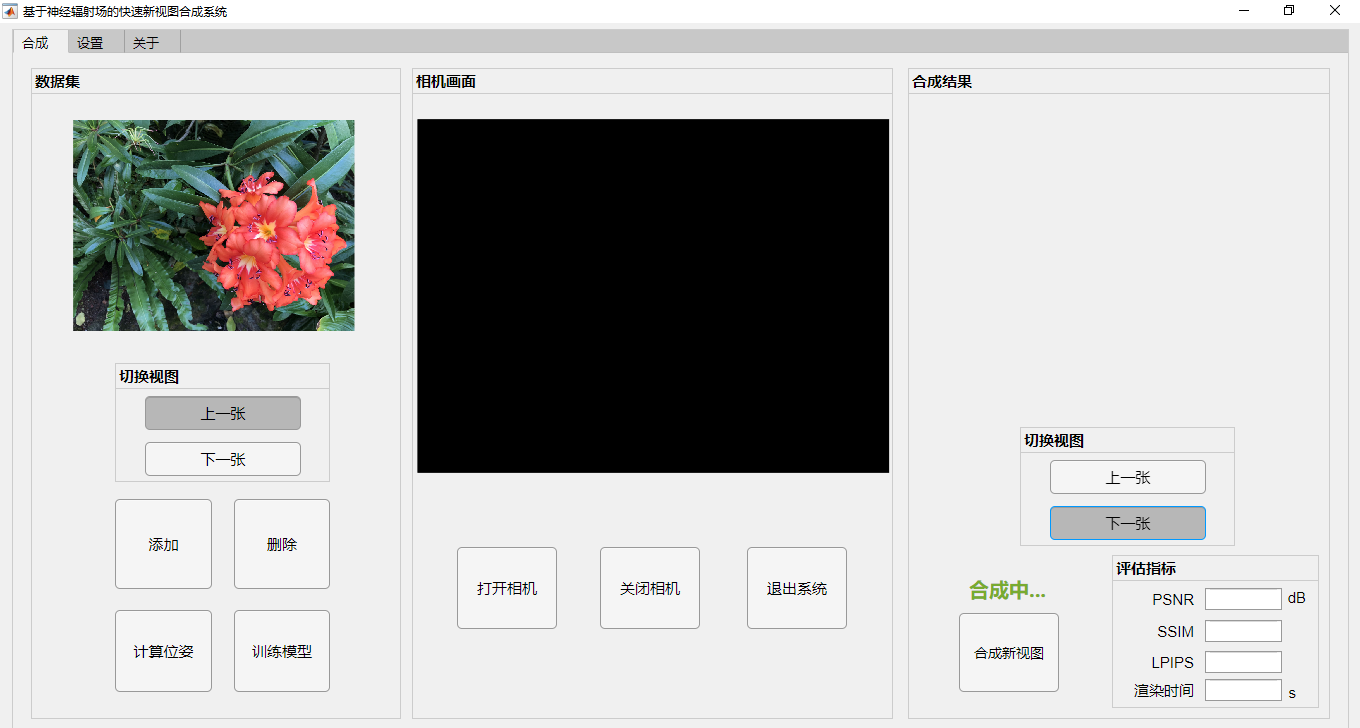
\includegraphics[width=0.45\linewidth]{figures/system/3-f.png}}
	\caption{新视图合成功能测试}
\end{figure}
\pagebreak
\begin{figure}[bhtp]
	\ContinuedFloat
	\centering
	\subcaptionbox{切换上一张已合成视图\label{fig:viewsynthesis-g}}
	{\includegraphics[width=0.45\linewidth]{figures/system/3-g.png}}
	\subcaptionbox{切换下一张已合成视图\label{fig:viewsynthesis-h}}
	{\includegraphics[width=0.45\linewidth]{figures/system/3-h.png}}
	\caption{(续) 新视图合成功能测试}
	\label{fig:viewsynthesis}
\end{figure}

\begin{figure}[htbp]
	\centering
	\includegraphics[width=0.95\linewidth]{figures/system/3-g.png}
	\caption{已合成的新视图,其中渲染时间为 \SI{4.23}{s}。}
	\label{fig:viewsynthesisBig}
\end{figure}
\section{本章小结}
本章主要介绍了基于神经辐射场的新视图快速合成系统的设计与实现。首先介绍了系统需求分析,包含功能性需求分析和非功能性需求分析,并展示了主要用例分析。然后阐述了此系统的基本设计架构以及将基于神经辐射场的新视图快速合成模型移植到 C++ 代码上的方法。之后介绍了系统的开发与运行环境。详尽地说明了经典测试用例的步骤,根据用例步骤完成了功能测试。从测试结果看,系统各项功能均能正常运行,合成新视图速度快且质量高。下一章将会对全文进行总结。
%本章主要介绍了基于神经辐射场的新视图快速合成系统的设计与实现。首先介绍了系统需求分析,并展示了主要用例分析。然后阐述了此系统的基本设计架构以及将本文的模型移植到 C++ 代码上的方法。之后介绍了系统的开发与运行环境。详尽地说明了经典测试用例的步骤,根据用例步骤完成了功能测试。从测试结果看,系统各项功能均能正常运行,合成新视图速度快且质量高。

\cleardoublepage

\cleardoublepage
%% !TeX root = ../main.tex

\chapter{系统的部署与展示}\label{figures_tables}
本节主要介绍本文系统的部署与测试。本文的系统是运行于 Windows 平台,具体的运行环境见表~\ref{tab:env2}。在运行系统之前需要编译和配置好相关运行库,比如 LibTorch、OpenCV、MYNTAI S1040-IR-120/Mono的 SDK。

\section{系统运行环境}
本系统的开发和运行环境如表~\ref{tab:env1} 和表~\ref{tab:env2} 所示,包含软件环境和硬件环境。图~\ref{fig:photo} 展示的是本系统的真实硬件环境以及相应的系统交互界面。
\begin{table}[thbp]
	\centering
	\small\def\arraystretch{2.5}\setlength\tabcolsep{0.10\textwidth}
	\caption{系统开发环境}
	\begin{tabular}{|c|c|}
		\hline
		\multicolumn{2}{|c|}{软件环境}                \\
		\hline
		操作系统   & Ubuntu 18.04 \\
		\hline
		开发语言   & python、C++、matlab \\
		\hline
		运行环境  & python 3.6    \\
		\hline
		\multicolumn{2}{|c|}{硬件环境} \\
		\hline
		处理器    &      Intel(R) Core(TM) i5-4210U CPU @ 2.50 GHz  \\
		\hline
		内存      &       8GB         \\
		\hline
		显卡    &     TITAN X       \\
		\hline
	\end{tabular}
	\label{tab:env1}
\end{table}

\begin{table}[thbp]
  \centering
  \small\def\arraystretch{2.}\setlength\tabcolsep{0.06\textwidth}
  \caption{系统运行环境}
  \begin{tabular}{|c|c|}
    \hline
    \multicolumn{2}{|c|}{软件环境}                \\
    \hline
    操作系统   & Windows 10 					  \\
    \hline
    开发工具  & Matlab 2018b  					   \\
    \hline
    运行库   & LibTorch、OpenCV、MYNTAI S1040-IR-120/Mono SDK \\
    \hline
    \multicolumn{2}{|c|}{硬件环境} \\
    \hline
    处理器    &      Intel(R) Core(TM) i5-4210U CPU @ 2.50 GHz  \\
    \hline
    内存      &       8GB         \\
    \hline
    传感器    &     MYNTAI S1040-IR-120/Mono          \\
    \hline
  \end{tabular}
  \label{tab:env2}
\end{table}

\begin{figure}[htbp]
	\centering
	\includegraphics[width=0.95\linewidth]{figures/system-hardware.jpg}
	\caption{系统的硬件环境}
	\label{fig:photo}
\end{figure}
\pagebreak
\section{系统功能测试}
本小节针对本系统的各个模块进行测试,下面将详述测试的过程,并展示与用户交互的界面以及最终测试的结果。
\subsection{相机交互功能}
首先我们先测试电脑与相机方面的交互功能。与相机能够友好交互,获得稳定高质量的图像,这对整个训练或者测试都是意义重大地。相机传感器是数据的本源,是一切计算机视觉的基础和灵魂。拥有着一个鲁棒而友好的相机交互环境能为新视图合成任务提供非常好的输入,容易让网络学习到更准确的神经辐射场,预测出更准的颜色和体密度,这些都会在 PSNR、SSIM、LPIPS等指标上面体现出来。

\begin{table}[thbp]
  \centering
  \small\def\arraystretch{1.5}\setlength\tabcolsep{0.05\textwidth}
  \caption{相机交互功能测试用例}
  \begin{tabular}{|p{2cm}<{\centering}|p{4cm}<{\centering}|p{4cm}<{\centering}|}
    \hline
    用例编号 & \multicolumn{2}{|l|}{001}       \\
    \hline
    测试功能 & \multicolumn{2}{|l|}{相机交互}       \\
    \hline
    编号 & 输入/动作 & 期望结果 \\
    \hline
    1 & 打开应用,进入合成界面,在相机画面栏点击打开相机按钮 & 跳转到传感器 RGBD 相机界面 \\
    \hline
    2 & 在数据集栏点击添加按钮 & 当前相机的图像被捕获到数据集栏 \\
    \hline
    3 & 在相机画面栏点击关闭相机 & 提示:“您确定要关闭相机吗?” \\
    \hline
    4 & 点击确认关闭 & 相机画面终止 \\
    \hline
    5 & 点击取消关闭 & 整个交互界面不变 \\
    \hline
    6 & 点击退出系统 & 提示:“您确定退出吗?” \\
    \hline
    7 & 点击确认退出 & 整个交互界面退出 \\
    \hline
    8 & 点击取消退出 & 整个交互界面不变 \\
    \hline
  \end{tabular}
  \label{tab:camera}
\end{table}
根据表~\ref{tab:camera},整个数据集处理的测试步骤如下:
\begin{enumerate}
    \item[1)] 打开应用进入合成菜单栏,点击打开相机按钮,测试结果如图~\ref{fig:camara-a} 和图~\ref{fig:camara-b}。用例001编号为1的测试符合预期结果。
    \item[2)] 在数据集面板上点击添加,当前相机画面会被捕获到数据集,具体测试如图~\ref{fig:camara-c}。用例001编号为2的测试符合预期结果。
    \item[3)] 若点击了相机界面的关闭相机按钮,会有相应提示信息,如图~\ref{fig:camara-d} 所示。若点击是,则相机画面终止,如图~\ref{fig:camara-e} 所示。若点击否,则保持不变,如图~\ref{fig:camara-c}。用例001编号为3、4、5的测试符合预期结果。
    \item[4)] 若点击了相机界面的退出系统按钮,会有相应提示信息,如图~\ref{fig:camara-f} 所示。若点击是,则程序画面终止。若点击否,则保持不变,如图~\ref{fig:camara-e}。用例001编号为6、7、8的测试符合预期结果。
\end{enumerate}

\begin{figure}[bhtp]
  \centering
  \subcaptionbox{\label{fig:camara-a}}
    {\includegraphics[width=0.45\linewidth]{figures/system/1-a.png}}
  \subcaptionbox{\label{fig:camara-b}}
    {\includegraphics[width=0.45\linewidth]{figures/system/1-b.png}} \\
  \subcaptionbox{\label{fig:camara-c}}
    {\includegraphics[width=0.45\linewidth]{figures/system/1-c.png}}
  \subcaptionbox{\label{fig:camara-d}}
    {\includegraphics[width=0.45\linewidth]{figures/system/1-d.png}} \\
  \subcaptionbox{\label{fig:camara-e}}
    {\includegraphics[width=0.45\linewidth]{figures/system/1-e.png}}
  \subcaptionbox{\label{fig:camara-f}}
    {\includegraphics[width=0.45\linewidth]{figures/system/1-f.png}}
  \caption{相机交互功能测试}
  \label{fig:camara}
\end{figure}
\newpage

\subsection{数据集处理功能}
数据集处理是整个系统的最先使用的功能,非常至关重要,数据的选取决定了最终测试结果的好坏。数据集处理对应于本系统数据处理模块的功能。首先介绍下数据处理模块对应的典型测试用例,主要包含数据集的获取,删除。

\begin{table}[t]
  \centering
  \small\def\arraystretch{1.3}\setlength\tabcolsep{0.05\textwidth}
  \caption{数据集处理功能测试用例}
  \begin{tabular}{|p{2cm}<{\centering}|p{4cm}<{\centering}|p{4cm}<{\centering}|}
    \hline
    用例编号 & \multicolumn{2}{|l|}{002}       \\
    \hline
    测试功能 & \multicolumn{2}{|l|}{数据集处理}       \\
    \hline
    编号 & 输入/动作 & 期望结果 \\
    \hline
    1 & 打开应用,进入合成界面,在相机画面栏点击打开相机按钮 & 跳转到传感器 RGBD 相机界面 \\
    \hline
    2 & 在数据集栏点击添加按钮 & 当前相机的 RGB 数据被选作数据集并显示在数据集栏上 \\
    \hline
    3 & 在数据集栏点击上(下)一张按钮 & 数据集栏画面切换为上(下)一张图像 \\
    \hline
    4 & 在数据集栏点击删除按钮 & 提示:“您确定删除吗?” \\
    \hline
    5 & 点击确认删除 & 数据集栏当前显示的图像被删除 \\
    \hline
    6 & 点击取消删除或者提示栏右上角$\times$ & 数据集栏当前显示的图像被保留在数据集中 \\
    \hline
  \end{tabular}
  \label{tab:getdataset}
\end{table}

根据表~\ref{tab:getdataset},整个数据集处理的测试步骤如下:
\begin{enumerate}
    \item[1)] 打开应用进入合成菜单栏,点击打开相机按钮,测试结果如图~\ref{fig:camara-b}。用例002编号为1的测试与预期结果相符。
    \item[2)] 在数据集面板上点击添加,当前相机画面会被捕获到数据集,如图~\ref{fig:camara-c}。用例002编号为2的测试符合预期结果。
    \item[3)] 若点击数据集栏上(下)一张按钮,视图会切换到上(下)一张图像,如图~\ref{fig:datasetProcess-a} 和图~\ref{fig:datasetProcess-b}。用例002编号为3的测试符合预期结果。
    \item[4)] 若在数据集栏点击了删除按钮,会有相应提示信息,如图~\ref{fig:datasetProcess-c}。若点击是,则数据集当前画面终止,如图~\ref{fig:datasetProcess-d} 所示。若点击否,则保持不变,如图~\ref{fig:camara-e}。用例002编号为4、5、6的测试符合预期结果。
\end{enumerate}

\begin{figure}[thbp]
  \centering
  \subcaptionbox{\label{fig:datasetProcess-a}}
    {\includegraphics[width=0.55\linewidth]{figures/system/2-a.png}}
  \subcaptionbox{\label{fig:datasetProcess-b}}
    {\includegraphics[width=0.55\linewidth]{figures/system/2-b.png}}
  \subcaptionbox{\label{fig:datasetProcess-c}}
    {\includegraphics[width=0.55\linewidth]{figures/system/2-c.png}}
  \subcaptionbox{\label{fig:datasetProcess-d}}
    {\includegraphics[width=0.55\linewidth]{figures/system/2-d.png}}
  \caption{数据集处理功能测试}
  \label{fig:datasetProcess}
\end{figure}

\subsection{新视图合成功能测试}
基于之前的功能测试,对于本系统的任务来说并不够,因为还没有检验本文方法的可行性与效率。基于神经辐射场的快速新视图合成,最终必须落脚于新视图合成,并对其进行加速。下面是整个系统的最后一部分测试了,是为检测本文整个方法的性能,包含渲染速度以及渲染质量(包含PSNR、SSIM、LPIPS)等指标。通过多方面去表征本系统能有效地对 NeRF 进行加速。
\begin{table}[htbp]
  \centering
  \small\def\arraystretch{1.5}\setlength\tabcolsep{0.05\textwidth}
  \caption{新视图合成功能测试用例}
  \begin{tabular}{|p{2cm}<{\centering}|p{4cm}<{\centering}|p{4cm}<{\centering}|}
    \hline
    用例编号 & \multicolumn{2}{|l|}{003}       \\
    \hline
    测试功能 & \multicolumn{2}{|l|}{新视图合成}       \\
    \hline
    编号 & 输入/动作 & 期望结果 \\
    \hline
    1 & 点击计算位姿按钮 &  进度条提示计算位姿的过程 \\
    \hline
    2 & 点击训练模型按钮 &  进度条提示模型训练的过程 \\
    \hline
    3 & 点击合成新视图按钮 & 状态提示从待合成到合成中再到已合成 \\
    \hline
    4 & 在合成栏点击上(下)一张按钮 & 数据集栏画面切换为上(下)一张图像,并显示相应的指标信息 \\
    \hline
  \end{tabular}
  \label{tab:viewsynthesis}
\end{table}
根据表~\ref{tab:viewsynthesis},整个新视图功能测试的详细步骤如下:
\begin{enumerate}
    \item[1)] 若点击计算位姿按钮,会有相应提示信息,如图~\ref{fig:viewsynthesis-a} 和图~\ref{fig:viewsynthesis-b} 所示。用例003编号为1的测试与预期结果相符。
    \item[2)] 若点击训练模型按钮,会有相应提示信息,如图~\ref{fig:viewsynthesis-c} 和图~\ref{fig:viewsynthesis-d} 所示。用例003编号为2的测试与预期结果相符。
    \item[3)] 若点击合成新视图按钮,会有标签提示进度,如图~\ref{fig:viewsynthesis-e} 和图~\ref{fig:viewsynthesis-f} 以及图\ref{fig:viewsynthesis-g}。用例003编号为3的测试与预期结果相符。
    \item[4)] 若点击数据集栏上(下)一张按钮,视图会切换到上(下)一张图像,如图~\ref{fig:viewsynthesis-h}(上)和图~\ref{fig:viewsynthesis-g}(下)所示。用例002编号为4的测试与预期结果相符。
\end{enumerate}
\newpage

\begin{figure}[bhtp]
  \centering
  \subcaptionbox{\label{fig:viewsynthesis-a}}
    {\includegraphics[width=0.45\linewidth]{figures/system/3-a.png}}
  \subcaptionbox{\label{fig:viewsynthesis-b}}
    {\includegraphics[width=0.45\linewidth]{figures/system/3-b.png}}
  \subcaptionbox{\label{fig:viewsynthesis-c}}
    {\includegraphics[width=0.45\linewidth]{figures/system/3-c.png}}
  \subcaptionbox{\label{fig:viewsynthesis-d}}
    {\includegraphics[width=0.45\linewidth]{figures/system/3-d.png}}
  \subcaptionbox{\label{fig:viewsynthesis-e}}
    {\includegraphics[width=0.45\linewidth]{figures/system/3-e.png}}
  \subcaptionbox{\label{fig:viewsynthesis-f}}
    {\includegraphics[width=0.45\linewidth]{figures/system/3-f.png}}
  \subcaptionbox{\label{fig:viewsynthesis-g}}
    {\includegraphics[width=0.45\linewidth]{figures/system/3-g.png}}
    \subcaptionbox{\label{fig:viewsynthesis-h}}
    {\includegraphics[width=0.45\linewidth]{figures/system/3-h.png}}
  \caption{新视图合成功能测试}
  \label{fig:viewsynthesis}
\end{figure}
\newpage
\section{本章小结}
本章主要介绍了基于神经辐射场的新视图快速合成系统的部署与展示。首先介绍了系统的开发与运行环境。详尽地说明了经典测试用例的步骤,根据用例步骤完成了功能测试。从测试结果看,系统各项功能均能正常运行,合成新视图速度快且质量高。下一章将会对全文进行总结。

% \section{插图}

% 图片通常在 \env{figure} 环境中使用 \cs{includegraphics} 插入,如图~\ref{fig:example} 的源代码。
% 建议矢量图片使用 PDF 格式,比如数据可视化的绘图;
% 照片应使用 JPG 格式;
% 其他的栅格图应使用无损的 PNG 格式。
% 注意,LaTeX 不支持 TIFF 格式;EPS 格式已经过时。

% 图片的标题应置于图片下方。

% \begin{figure}
%   \centering
%   \includegraphics[width=0.6\linewidth]{example-image-a.pdf}
%   \caption{示例图片}
%   \label{fig:example}
% \end{figure}

% 若图或表中有附注,采用英文小写字母顺序编号,附注写在图或表的下方。
% % LaTeX 传统上一般将附注的内容同图表的标题写在一起,形成很长的一段文字。

% 如果一个图由两个或两个以上分图组成时,各分图分别以(a)、(b)、(c)...... 作为图序,并须有分图题。
% 推荐使用 \pkg{subcaption} 宏包来处理, 比如图~\ref{fig:subfig-a} 和图~\ref{fig:subfig-b}。

% \begin{figure}
%   \centering
%   \subcaptionbox{分图 A\label{fig:subfig-a}}
%     {\includegraphics[width=0.45\linewidth]{example-image-a.pdf}}
%   \subcaptionbox{分图 B\label{fig:subfig-b}}
%     {\includegraphics[width=0.45\linewidth]{example-image-b.pdf}}
%   \caption{多个分图的示例}
%   \label{fig:multi-image}
% \end{figure}


% \section{表格}

% 表应具有自明性。为使表格简洁易读,尽可能采用三线表,如表~\ref{tab:three-line}。
% 三条线可以使用 \pkg{booktabs} 宏包提供的命令生成。

% 表格的标题应置于表格上方。

% \begin{table}
%   \centering
%   \caption{三线表示例}
%   \begin{tabular}{ll}
%     \toprule
%     文件名          & 描述                         \\
%     \midrule
%     thuthesis.dtx   & 模板的源文件,包括文档和注释 \\
%     thuthesis.cls   & 模板文件                     \\
%     thuthesis-*.bst & BibTeX 参考文献表样式文件    \\
%     thuthesis-*.bbx & BibLaTeX 参考文献表样式文件  \\
%     thuthesis-*.cbx & BibLaTeX 引用样式文件        \\
%     \bottomrule
%   \end{tabular}
%   \label{tab:three-line}
% \end{table}

% 表格如果有附注,尤其是需要在表格中进行标注时,可以使用 \pkg{threeparttable} 宏包,
% 用英文小写字母 a、b、c……顺序编号。

% \begin{table}
%   \centering
%   \begin{threeparttable}[c]
%     \caption{带附注的表格示例}
%     \label{tab:three-part-table}
%     \begin{tabular}{ll}
%       \toprule
%       文件名                 & 描述                         \\
%       \midrule
%       thuthesis.dtx\tnote{a} & 模板的源文件,包括文档和注释 \\
%       thuthesis.cls\tnote{b} & 模板文件                     \\
%       thuthesis-*.bst        & BibTeX 参考文献表样式文件    \\
%       thuthesis-*.bbx        & BibLaTeX 参考文献表样式文件  \\
%       thuthesis-*.cbx        & BibLaTeX 引用样式文件        \\
%       \bottomrule
%     \end{tabular}
%     \begin{tablenotes}
%       \item [a] 可以通过 xelatex 编译生成模板的使用说明文档;
%         使用 xetex 编译 \file{thuthesis.ins} 时则会从 \file{.dtx} 中去除掉文档和注释,得到精简的 \file{.cls} 文件。
%       \item [b] 更新模板时,一定要记得编译生成 \file{.cls} 文件,否则编译论文时载入的依然是旧版的模板。
%     \end{tablenotes}
%   \end{threeparttable}
% \end{table}

\cleardoublepage

%\cleardoublepage
% TEX-root = ../main.tex
\chapter{总结与展望}
本章将总结本文现有的工作,并对未来的可能的研究方向进行展望。
\section{总结}
当前虚拟现实、自由视点视频、街景地图等领域对新视图合成存在大量需求,通过对现有的相关系统进行调研发现存在以下问题:1) 当前市场上的三维渲染的软件难以根据稀疏视图,在任意视角下渲染出高质量的新视图;
2) 目前的三维渲染系统大都需要根据深度信息进行三维建模,这需要使用 RGBD 相机,对硬件设备要求较高;
3) 目前市场上还没有直接可应用的面向快速新视图合成的交互系统;4) 现有的新视图合成模型需要在空间内进行大量采样,计算时间成本较高,难以完成 PC 端的交互需求。在这样的背景下,本文结合 NeRF 的技术以及查询表缓存加速的相关技术实现了快速合成新视图的神经辐射场渲染具体方法,并设计和实现了一个快速新视图合成的系统,完成了 PC 客户端的相关应用。

本文的主要工作与贡献如下:

\begin{enumerate}
	\item [1)] 本文基于 NeRF 预训练的网络预测的体密度信息构建出一个可以表征在物体内外的查询表结构,这一方面直接减少了查询表的尺寸,另一方面该查询表可以直接为空间内任意一点提供 NeRF 网络中间层的特征,这加快了神经网络的正向传播速度。
	\item [2)] 在缓存了上述查询表的基础上,本文改进了 NeRF 的采样过程,通过查询表找到光线上离物体表面最近的内点,使得 NeRF 可以仅在此点附近进行采样,从而不必再使用两个网络,这显著加速了 NeRF。
	\item [3)] 为了补偿查询表分辨率不够带来的精度损失,本文对 F-NeRF 进行再训练,将渲染质量提升到原 NeRF 的水平。
	\item [4)] 本文在公开的数据集上做了大量对比验证实验。在公开合成数据集 Synthetic-NeRF 和真实场景数据集 LLFF-NeRF 上,与 NeRF 相比,我们提出的 F-NeRF 方法分别加速 3.2 倍和 3.4倍。 
	\item [5)] 本文设计并实现了基于 NeRF 的快速新视图合成的系统,完成了相应的 PC 端的应用,并对该系统进行了详细的需求分析以及架构设计,最后将本文的方法实现并部署到了 PC 端,经过详细地测试,该系统满足实际应用需求。
\end{enumerate}


\section{展望}
本文实现的基于神经辐射场的快速新视图合成系统保留了人机交互的自然、简洁等优点,并保证了交互的一致性与实时性,具有一定的应用前景。但系统仍存在一些值得思考与完善的地方:
\begin{enumerate}
	\item 本文基于 NeRF 改进的快速新视图合成方法本质还是假设输入图像为静态图像,然而在真实场景里,这是很难做到的。因此在未来希望通过改进算法使得系统输入动态图像也可以合成较高质量的视图。
	\item 目前本系统的方法使用的查询表提取到的物体几何信息不够准确,这是因为缓存的点过于稀疏,对于空洞较多的场景渲染出的新视图质量不够好。因此在未来可以借助 mesh 缓存场景的几何信息,使用 ray tracing 的方法去找到物体表面,从而可以更好地优化采样点的位置。
	\item 由于测试的时候还是使用了神经网络,因此本系统还不足以做到实时的合成新视图。因此未来可以转换思路,从缓存网络参数到直接缓存输出的颜色和体密度,这样可以让测试的过程与神经网络解耦,从而地合成新视图。
\end{enumerate}

















% \begin{enumerate}
%     \item \texttt{sysusetup.tex}: 填写标题、作者、导师、学位名称等信息。
%     \item \texttt{data/abstract.tex}: 填写中英文摘要。
%     \item \texttt{data/denotation.tex}: 填写符号与缩略语,注意按音序排序。
%     \item \texttt{data/chapxx.tex}: 各章内容,如有章节增删请在\texttt{main.tex}中修改相关记录。
%     \item \texttt{data/appendix.tex}: 附录。
%     \item \texttt{data/works.tex}: 学术成果。
%     \item \texttt{data/acknowledgements.tex}: 致谢。
%     \item \texttt{ref/refs.bib}: 引文数据库。
%     \item \texttt{main.tex}: 主文件,用于控制文档选项(字体,学位类别):
%     \begin{enumerate}
%         \item 学术硕士: \verb|\documentclass[degree=master]{sysuthesis}|;
%         \item 专业硕士: \verb|\documentclass[degree=master,degree-type=professional]{sysuthesis}|;
%         \item 博士: \verb|\documentclass[degree=doctor]{sysuthesis}|。
%     \end{enumerate}
%     指定论文要包括的部分,如摘要、目录、正文各章节、附录、引文数据库等等。
%     (注意插入每章内容之后要加 \verb|\cleardoublepage| 以保证在打印版中各章都从右边开始):
%     \begin{verbatim}
%     % !TeX root = ../main.tex

\chapter{绪论}

本章作为绪论主要介绍了神经辐射场中新视图合成加速问题的背景与意义,分析了目前相关技术与算法的发展现状以及相关系统存在的问题,阐述了解决该问题的必要性,然后总结了本文的主要工作与贡献,最后概述了本文的章节结构。

\section{研究背景与意义}
近年来,随着深度学习与计算机视觉的飞速发展,人类的生活愈来愈趋向智能化。在以前,人们必须通过行万里路来了解这个世界,但是现在,可以通过全景地图几乎全方位地去观察一个未知的地方,甚至是通过虚拟现实,增强现实等形式沉浸式地以任意的角度呈现出场景或者物体。新视图合成技术可以支持以上应用场景,可以通过已有的图像去合成新视角下的图像。

新视图合成任务\cite{chen1993view}作为计算机视觉和计算机图形学的交叉领域任务,有着极其广阔的应用前景,一直是学术界和工业界的热门研究问题。新视图合成任务具体是,通过给定的已知视角下观测到的图像,去合成新视角下的图像。图~\ref{fig:FreeViewSynthesis} 给出了新视图合成任务的示意图。

\begin{figure}[tbhp]
    \centering
    \includegraphics[width=0.95\textwidth]{figures/FreeViewSynthesis.pdf}
    \caption{新视图合成的示意图\cite{riegler2020free}。前三张图是合成的新视图,最后一张图阐明了绿色相机位姿下的图像作为输入,推理红色相机位姿的新视图。}
    \label{fig:FreeViewSynthesis}
\end{figure}
\newpage

根据前期调研,新视图合成技术有着广泛的应用前景,市场需求庞大,急需可快速合成高质量新视图的系统。而在实际应用中,限于应用需求和经济成本等因素的考量,市场上的大多产品仍存在着许多问题,比如无法在任意角度合成高质量图像,另外渲染新视图的时间过长,这些都严重影响了用户体验。而本身,三维场景具有一定复杂性,市面上的很多软件在渲染之前需要进行复杂的三维建模,这很考验硬件的算力和内存。这些都增加了系统的实现难度。

具体地,现有的系统中存在以下一些问题:1) 当前市场上的三维渲染的软件难以根据稀疏视图,在任意视角下渲染出高质量的新视图;
2) 目前的三维渲染系统大都需要根据深度信息进行三维建模,这需要使用 RGBD 相机,对硬件设备要求较高;
3) 目前市场上还没有直接可应用的面向快速新视图合成的交互系统;4) 现有的新视图合成模型需要在空间内进行大量采样,计算时间成本较高,难以完成 PC 端的快速交互需求。

如果想要把新视图合成技术很好地应用在虚拟现实等技术上,那么必须能够在任意视角下合成几乎与真实场景相同的图像。这在合成场景下是可能实现的,但是在真实场景中,无法获得准确的相机位姿、光照条件难以建模等问题都限制了更好的体验,新视图合成仍面临着许多挑战。

% 主要挑战是通过给定稀疏的观测图像来推断场景的三维几何结构,以及对场景中遮挡和看不见的地方进行修补。在经典计算机视觉中,基于图像的渲染 (Image-based Rendering, IBR\cite{debevec1998efficient,kee2013exposing}) 方法通常依赖于基于优化的多视图立体 (Multi-View Stereo, MVS) 方法,以将重构场景的几何形状并将观测转到新视图的坐标系中。然而,如果只有少量观测图像可用,场景包含依赖视图的影响或者新视角下大部分没有被观测的图像覆盖到,那么 IBR 可能失效会导致出现鬼影或者空洞等效果。最近,随着深度学习的发展,基于深度学习的神经渲染方法\cite{tewari2020state}被提出,旨在合成更高质量的新视图。2020年,Mildenhall等人\cite{mildenhall2020nerf}提出了基于神经辐射场 (Neural Radiance Fields, NeRF) 的方法去合成新视图,这使得神经渲染一度成为最优秀的新视图合成方法。NeRF 基于给定的稀疏图像,仅使用较为简单的全连接网络去隐式表达场景信息,最后使用体绘制的方法合成新视图。NeRF 是目前新视图合成任务中的渲染效果最佳的方法,但是由于使用体绘制进行渲染,要求必须在空间内进行大规模采样,这一方面会带来巨大的时间开销,另一方面采样点的位置的准确性将决定了神经辐射场拟合的准确性。



经典的基于图像的渲染 (Image-based Rendering, IBR\cite{kee2013exposing}) 方法可以完成以上任务,IBR 通常依赖于基于优化的多视图立体 (Multi-View Stereo, MVS) 方法,以此重构场景的几何结构。然而,如果只有少量观测图像可用,场景包含依赖视图的影响或者新视角下大部分没有被观测的图像覆盖到,那么 IBR 可能失效会导致出现鬼影或者空洞等效果。此外该方法需要对三维场景进行精细的三维重建,这会带来极大的计算开销,因此传统的基于图像的渲染方法难以应用到实际场景中。随着深度学习的发展,基于深度学习的神经渲染方法开始在新视图合成任务上展现出其惊人的渲染效果。
2020年,Mildenhall等人\cite{mildenhall2020nerf}提出了基于神经辐射场 (Neural Radiance Fields, NeRF) 的方法去合成新视图,这使得神经渲染一度成为最优秀的新视图合成方法。NeRF 基于给定的稀疏图像,仅使用较为简单的全连接网络去隐式表达场景信息,最后使用体绘制的方法合成新视图。如果有一个系统能够使用基于 NeRF 的方法快速渲染出高质量的新视图,那么将极大地提升用户体验。因此,在这样的需求下,本文致力于将具有最佳渲染效果的 NeRF 技术设计并实现成完整的新视图合成系统,并在不损失精度的情况下对其渲染过程进行加速。

NeRF 是目前新视图合成任务中的渲染效果最佳的方法,但是由于使用体绘制进行渲染,要求必须在空间内进行大规模采样,这一方面会带来巨大的时间开销,另一方面采样点的位置的准确性将决定了神经辐射场拟合的准确性。

本文主要关注的是渲染时间长这一问题。NeRF 为了获取对渲染图象贡献较高的采样点,同时优化两个神经网络,使用 coarse 网络的输出去估计采样点的分布情况,然后基于此分布进行二次采样并通过 fine 网络预测的颜色和体密度进行数值积分计算出 2D 图像对应像素的 RGB 值,这带来了极大的时间开销。同时为了拟合更准确的神经辐射场,NeRF 使用了较深的神经网络,这也增加了推理新视图过程的时间成本。以上正是本文需要加速的地方。

在这样的背景下,本文研究了基于神经辐射场的新视图合成的相关技术,认为基于深度学习的神经渲染方法存在着提升空间,并对现有方法 NeRF 进行了优化,设计并训练了可以快速合成高质量新视图的神经渲染模型。渲染效果受数据集的影响,一般来说合成场景下质量会相对好些,因为真实场景下问题比较多,比如相机标定不严格、相机位姿估计不准,照片畸变严重,光照条件难以建模等等。

最终,本文结合 NeRF 的技术以及查询表缓存加速的相关技术实现了快速合成新视图的神经辐射场渲染具体方法,并设计和实现了一个快速新视图合成的系统,完成了 PC 客户端的相关应用。与现有产品相比,该系统可以基于给定的稀疏图像,快速渲染出任意新视角下的图像,提供几乎和 NeRF 质量相同的新视图。

本课题来自于PixTalks公司的实际应用需求。

\section{国内外研究现状}
% \subsection{新视图合成相关系统应用现状}
% 为了了解新视图合成相关系统的现状,本文对相关产品进行了调研。目前市面上暂无直接具有新视图合成功能的系统或软件,都是将新视图合成技术嵌入到系统或软件的内部。    

\subsection{基于图像的神经渲染方法研究现状}
在计算机图形和计算机视觉中,基于图像的渲染方法通常是依靠场景的一组二维图像来生成三维模型,然后渲染该场景的一些新视图。一般基于图像的渲染 (Image-based Rendering, IBR) 方法根据是否使用几何信息分成两类。几何信息用于将图像内容从捕获的图像重新投影到新的目标图像域。在目标图像域中,源图像的投影被混合以合成最终图像。这种简化的过程仅能为具有精确几何结构且具有捕获足够多视图的物体提供较为准确的结果。但是,由于依赖于视图的影响,以及不完善的几何信息或太少的源图像,可能会出现诸如重影,模糊,孔洞或接缝之类的伪影。

\begin{figure}[tbhp]
    \centering
    \includegraphics[width=0.95\textwidth]{figures/deepblending.pdf}
    \caption{DeepBlending\cite{hedman2018deep} 的框架结构,渲染效果较其他方法减少了伪影。}
    \label{fig:deepblending}
\end{figure}

为了解决上述问题,将经典的基于图像渲染的方法与现如今最火的深度学习网络的结合成基于 IBR 的神经渲染方法,这极大地提升了 IBR 的渲染效果。DeepBlending\cite{hedman2018deep}提出了一种广义网络来预测投影源图像的混合权重,以便在目标图像空间进行合成。DeepBlending 在室内场景中显示了惊人的效果,比经典的 IBR 方法具有更少的混合伪影,具体见图~\ref{fig:deepblending}。事实上,DeepBlending 是将 COLMAP\cite{schonberger2016structure} 和商用软件 Reality Capture 进行了结合,以此获取更为精细的几何结构信息。COLMAP 基于块匹配的多视图几何算法进行稠密重建,这能够非常好地重建场景中的细节,但是与此同时在纹理信息缺失的地方也会出现空洞。Reality Capture 的结果相对完整,但是对于场景级别的区域重建的较差。因此,上述两种方法是互补的,将它们进行结合可以获得非较为准确的几何模型信息,DeepBlending 就是使用上述几何信息,借助神经网络来学习如何将不一致的观测图像信息进行混合,最终确实获得了非常惊艳的效果。但是,该方法过于依赖 COLMAP 三维重建出的几何信息,当几何信息较少时渲染质量会严重下降并伴随伪影。此外,精细的三维重建会带来非常大的计算开销,这在实际中难以使用。因此这种经典的基于 IBR 的方法无法满足本系统的速度和质量需求。

%其他方法如 NPBG\cite{aliev2019neural} 和 NPCR\cite{dai2020neural} 使用比 mesh 更容易获得的点云作为三维代理几何体。由于点云自身的稀疏性特征,很可能会出现不应该观测到的点出现在新视角下,这是著名的 bleeding 现象。为了解决 bleeding 现象问题,NPBG 使用多分辨率的方式,将不同分辨率的特征图输入到后端网络中。不过,多分辨率的策略虽然解决了 bleeding 的问题,但是得到了相对模糊的渲染结果。	

\subsection{基于 NeRF 的新视图合成研究现状}
类似 DeepSDF\cite{park2019deepsdf},NeRF\cite{mildenhall2020nerf}借助深度学习的隐式表达方法,将三维几何场景中的光照和几何信息隐式表达在神经网络参数中,最后利用立体渲染的方法进行渲染。NeRF 算是基于图像的神经渲染方法中最具代表的工作了。NeRF 本身不需要任何的显式的几何信息,仅使用真实场景的 RGB 图像作为监督信号,使用深度神经网络自动推理相关几何以及光照信息。NeRF 凭借着其网络简单,渲染效果惊艳的特性,备受学术界和工业界的关注。自从 NeRF 的出现,基于神经辐射场的新视图合成相关工作开始大量涌现。

NeRF++\cite{zhang2020nerf++} 首次指出 NeRF 具有形状光线的歧义性问题,即 NeRF 在一个场景下训练好的网络,其对应的空间表示可能是错的,但是仍能在训练集上渲染出正确的结果。

%\begin{figure}[tbhp]
%    \centering
%    \includegraphics[width=0.95\textwidth]{figures/NeRF-W.pdf}
%    \caption{NeRF-W\cite{martin2020nerf}的网络框架示意图}
%    \label{fig:nerf-w}
%\end{figure}
%
%之后 NeRF-W\cite{martin2020nerf} (NeRF in the Wild) 对 NeRF 进行了另一种补充改进。由于 NeRF 假设输入的图像是由静态场景生成的图像,每张图所表示的场景具有相同的光照条件和几何结构,这在实际中是很难保证的。对于这个问题,如图~\ref{fig:nerf-w}所示,NeRF-W 给每张图片都预先编码了两个固定向量,分别是 $l_i^{\left(a\right)}, l_i^{\left(\tau\right)}$。其中,$l_i^{\left(a\right)}$ 是用来学习当前的光照条件,而 $l_i^{\left(\tau\right)}$ 是用来学习当前图像是否有动态物体遮挡,将这两个embedding 输入网络会输出一个不确定度。以上的做法让 NeRF-W 在真实场景下能够表现地更加鲁棒,在光照条件变化以及动态的场景下都取得了非常好的效果。

Yen-Chen等人\cite{yen2020inerf}基于位姿估计方法给 NeRF 提供了新的改进思路,推出了新工作 iNeRF。NeRF 在处理真是数据集的时候,位姿是通过COLMAP\cite{schonberger2016structure}进行计算的,然而这并不能获得绝对精准的位姿,也即送入网络的采样点是不准确的,那么也无法准确拟合真是场景的神经辐射场。如图~\ref{fig:inerf} 所示的是 iNeRF 的网络框架,注意到,颜色的均方误差对坐标是可微的,而坐标对相机位姿也是可微的,因此,可以在训练神经辐射场的同时对位姿进行优化,具体是采用神经网络的反向传播算法进行优化的。此外,为了更有效地优化位姿,iNeRF 使用了 ROI 采样方式,即对感兴趣的区域进行采样优化,这样能显著缓解直接采样一张图片带来的内存开销大的问题。iNeRF 通过位姿矫正,最终在真实场景下显著提升了 NeRF 的渲染质量。不过,由于训练时每一张图都要单独优化位姿,而渲染时相机位姿仍然是不准确的,因此本系统暂不考虑位姿的问题。

\begin{figure}[tbhp]
    \centering
    \includegraphics[width=0.95\textwidth]{figures/iNeRF.pdf}
    \caption{iNeRF\cite{yen2020inerf}的网络框架示意图}
    \label{fig:inerf}
\end{figure}

上述方法都还是基于多层感知机 (MLP, Multilayer Perceptron) 训练的。下面介绍一些对 NeRF 网络上进行的一些改进的工作。PixelNeRF\cite{yu2020pixelnerf} 使用卷积神经网络 (Convolutional Neural Networks, CNN) 提取的特征,仅需要少量图片作为输入就可以合成新视角下的图像,并有一定的泛化能力。GRF\cite{trevithick2020grf}使用 CNN 提取包含光线属性的特征,并使用 attention 机制将采样点在不同视角下的特征进行聚合,极大地提升了渲染质量。GRAF\cite{schwarz2020graf} 使用对抗生成网络 (Generative Adversarial Networks, GAN) 对 NeRF 进行改进,使之具有较强的泛化能力。但是,以上这些基于网络的改进方法都使得网络变得过于复杂,有些违背 NeRF 网络简洁的初衷,会使得训练和渲染的时间过长,这不能满足用户对于快速合成新视图的需求,几乎无法应用到实际的系统中。

\begin{figure}[htb]
	\centering
	\includegraphics[width=0.95\textwidth]{figures/NSVF.pdf}
	\caption{NSVF\cite{liu2020neural}的网络框架示意图}
	\label{fig:nsvf}
\end{figure}

下面介绍一些基于 NeRF 的加速方法。由于 NeRF 需要在相机光线上进行大量的采样,这些采样点都要经过网络,而 NeRF 自身又使用了两个网络进行训练,因此 NeRF 的渲染是很慢的。如图~\ref{fig:nsvf},为了给 NeRF 加速,NSVF\cite{liu2020neural} 首先提出将空间划分为若干体素,使用自我裁剪的方法去掉体密度较小的体素,渲染的时候只需找到相机光线第一个穿过的体素,根据该体素八个顶点对应的特征进行插值编码并送入下游 MLP 预测出颜色和体密度,这避免了大量的采样计算,显著加速了新视图合成的过程。但是,NSVF 仅适用于简单的三维物体,在复杂的真实场景下渲染新视图的质量较差,甚至会出现鬼影,因此并不适合在本系统上使用。Lindell等人\cite{lindell2020autoint}提出了一种利用自动积分来进行渲染加速的方法 AutoInt。AutoInt 是通过隐式网络学习到闭式解求积分,从而取代了 NeRF 的数值积分,最终能为 NeRF 渲染过程加速10倍。不过,就 PSNR 来看,AutoInt 在合成数据集 Synthetic-NeRF 上平均比 NeRF 低\SI{5.4}{dB},这是一种重视加速但牺牲了很多质量的方法,并没有真正做到在不失精度的情况下对渲染进行加速。上述介绍的加速方法未能保证不损失精度情况下对 NeRF 进行加速,不符合本系统的需求,因此本文最终依旧使用最经典应用场景最丰富的 NeRF 技术并对其进行无精度损失的加速,最终完成整个快速新视图合成系统的构建。

\section{本文的主要工作与贡献}
% 基于神经辐射场的快速新视图合成系统的设计与实现中存在以下一些问题:1) 当前市场上的三维渲染的软件难以根据稀疏视图,在任意视角下渲染出高质量的新视图;
% 2) 目前的三维渲染系统大都需要根据深度信息进行三维建模,这需要使用 RGBD 相机,对硬件设备要求较高;
% 3) 目前市场上还没有直接可应用的面向快速新视图合成的交互系统;4) 现有的新视图合成模型需要在空间内进行大量采样,计算时间成本较高,难以完成 PC 端的交互需求。

本文将 NeRF 技术和查询表技术进行有机融合,设计并实现了基于神经辐射场的快速新视图合成系统。本文根据 NeRF 的特性提出了基于神经辐射场进行加速合成新视图的框架, 将其命名为 F-NeRF,通过 NeRF 预测的体密度有效地提取到物体的几何结构并缓存到查询表中,这一方面辅助了获取物体表面附近的对计算颜色有高贡献的采样点,另一方面减少了一个网络的开销,同时也简化了网络,这显著加速了渲染的过程。最后,本文将这 F-NeRF 这一方法有效地部署到 PC 端,将其实现成可交互的系统。

具体地,本文的主要工作与贡献如下:
\begin{enumerate}
    \item [1)] 本文基于 NeRF 预训练的网络预测的体密度信息构建出一个可以表征在物体内外的查询表结构,这一方面直接减少了查询表的尺寸,另一方面该查询表可以直接为空间内任意一点提供 NeRF 网络中间层的特征,这加快了神经网络的正向传播速度。
    \item [2)] 在缓存了上述查询表的基础上,本文改进了 NeRF 的采样过程,通过查询表找到光线上离物体表面最近的内点,使得 NeRF 可以仅在此点附近进行采样,从而不必再使用两个网络,这显著加速了 NeRF,同时这正是本文的核心贡献。
    \item [3)] 为了补偿查询表分辨率不够带来的精度损失,本文对 F-NeRF 进行再训练,将渲染质量提升到原 NeRF 的水平。
    \item [4)] 本文在公开的数据集上做了大量对比验证实验。在公开合成数据集 Synthetic-NeRF 和真实场景数据集 LLFF-NeRF 上,与 NeRF 相比,我们提出的 F-NeRF 方法分别加速 3.2 倍和 3.4倍。 
    \item [5)] 本文设计并实现了基于 NeRF 的快速新视图合成的系统,完成了相应的 PC 端的应用,并对该系统进行了详细的需求分析以及架构设计,最后将本文的方法实现并部署到了 PC 端,经过详细地测试,该系统满足实际应用需求。
\end{enumerate}

%1) 使用预训练的 NeRF 网络,构建出一个可以表征在物体内外的查询表,该查询表可以直接为空间内任意一点提供 NeRF 网络中间层的特征,这加快了神经网络的正向传播速度。
%2) 在缓存了上述查询表的基础上,本文改进了 NeRF 的采样过程,通过查询表找到光线上离物体表面最近的内点,使得 NeRF 可以仅在此点附近进行采样,从而不必再使用两个网络,这显著加速了 NeRF,同时这正是本文的核心贡献。3) 本文设计并实现了基于 NeRF 的快速新视图合成的系统,完成了相应的 PC 端的应用,并对该系统进行了详细的需求分析以及架构设计,最后将本文的方法实现并部署到了 PC 端,经过详细地测试,本文方法在合成场景和真实场景下的渲染速度对 NeRF 分别加速3.2倍和3.4倍,该系统满足实际应用需求。


\section{本文的章节安排}

第一章是绪论,主要阐述了本文研究工作的背景与意义,指出了本文研究问题的难点,并介绍了本文的主要研究工作和贡献,对国内外相关工作的研究现状的充分调研与分析,最后对本文的组织架构进行安排。

第二章是相关理论和技术,主要介绍了基于神经辐射场的快速新视图合成系统应用的核心技术和算法。

第三章是本文的主要工作,主要介绍了本文方法的问题定义,本文方法的预备工作,然后详述了我们改进的基于神经辐射场的新视图合成加速方法。

第四章是本文的实验部分。主要阐述了实验的基本设置,包含开发环境、数据集等等,其次介绍了实验实现的具体细节以及相关评测指标。最后通过大量对比实验来验证本文提出的方法的有效性,同时对一些实验结果进行分析和讨论。

第五章是系统设计与实现,主要介绍了将本文提出的 F-NeRF 方法应用到系统上的具体实现与架构设计。详细阐述了本系统的需求分析,包含主要用例分析,以及具体的系统架构设计,最后介绍了将本系统的模型移植到 C++ 代码上的方法。

第六章是系统的部署与展示,主要介绍了本文系统的开发与运行环境,对经典的测试用例进行了详尽的步骤说明,根据用例步骤完成了功能测试。从测试结果看,系统各项功能均能正常运行,合成新视图速度快且质量高。

第七章为总结和展望部分。总结了本文的主要工作和贡献,并指出工作中的不足之处。提出在未来研究过程中的可能的研究方向,并对可继续完善的方面进行展望。
% \begin{enumerate}
%     \item 主体部分包括引言 (前言),国内外文献综述,正文, 结语,参考文献。要求图表清晰,叙述流畅,章节有序,层次 分明。\\
%     引言 (前言)部分内容主要为本研究课题的学术背景及理论与实际意义;本研究课题的来源及主要研究内容;建立研究的线索与思路。

%     \item 文中的图、表、公式等,一律用阿拉伯数字按章顺序编号。如图 1-1、图2-2, 表 1-1、表 2-1,公式 (1-1) 等。图序及图名置于图的下方,居中排列;表序及表名置于表的上方,居中排列。详见第\ref{figures_tables}章的说明。

%     \item 参考文献
%     \begin{enumerate}
%         \item 参考文献为论文中所有引文、引用观点以及对论文有重要影响和启发的文献;
%         \item 参考文献按在论文中出现的先后依次排序;个别学科若通用该学科惯用的排序规范,可以例外;
%         \item 参考文献内容一般排列在论文末尾 (论文篇幅较大且引用文献较多的,可在每章末尾注出),序码与论文加注处对应;
%         \item 参考文献标注格式: 使用国标GB/T 7714-2015标准, 建议使用工具自动控制引文格式, 
%         以保证格式规范。
%         该\LaTeX{}模板已经对引文格式做了配置,
%         用户需要将所需参考文献的信息存在 \texttt{bib} 格式的文件\texttt{ref/refs.bib}中, 
%         通过 \verb|\cite{}|命令在恰当位置引用 (详见第\ref{citations}章的说明)。
%         \texttt{bib}文件可从文献管理工具导出或自己用 \texttt{JabRef} 等软件编辑。
%     \end{enumerate}

%     \item 注释:可以用 “脚注”或 “文后注”来标注引用著作中的一些观点和案例,但全文标注方式应统一。
% \end{enumerate}


%     \cleardoublepage
%     % !TeX root = ../main.tex

\chapter{相关技术和理论概述}\label{equations}
本文主要研究的内容是神经辐射场在新视图合成上的加速,因此本章首先主要介绍神经三维形状表示法,新视图合成和基于图像的渲染方法。随着深度学习的发展,当今效果最佳的新视图合成算法都是基于深度学习的,因此接下来会概述深度学习的原理和发展状况,并重要介绍基于深度学习的神经辐射场的立体渲染方法。最后介绍一下查询表的概念,以及查询表在逐点网络上的加速应用,为本文方法的展开做好铺垫。

\section{神经三维形状表示法}
三维物体的形状表示有多种方法,传统的基于数据驱动的三维学习表示方法可以总体上分为三类:基于点,基于网格,基于体素的方法。此外,还有最新的基于深度学习的三维形状表示方法,下面对以上四种表示方法分别进行阐述。

\subsection{基于点的表示方法} 
基于点的方法一般指的是点云(如~\ref{fig:stanfordRabbit}所示的第一个)这种表示,点云是指空间中一组点的集合,每一个点都包含 X,Y,Z 三个坐标。它是一种轻量级的三维表示方式,与匹配许多传感器(例如雷达,深度相机)提供的原始数据非常匹配,因此非常适合应用在三维学习技术上。例如 PointNet\cite{qi2017pointnet,qi2017pointnet++} 这篇非常经典的点云工作,使用最大池化操作来提取全局特征,之后这项技术被广泛用作点生成网络\cite{yang2017foldingnet,achlioptas2018learning}的编码器。此后点云学习方面又涌入了大量的 PointNet 风格的相关工作。然而,点云这种表示方法有着很明确的限制,它们不适用于描述拓扑结构,同时也不适合用以生成紧致的表面。

\subsection{基于网格的表示方法}
许多方法使用预定义模板的网格,它们表征了一系列相似形状的物体,例如可变形的人体部位,其中一些模型\cite{2017Deformable}展示了高保真的形状生成结果。其他的最近工作\cite{baque2018geodesic}使用多边形立方体映射\cite{tarini2004polycube}对形状进行优化。虽然模板网格的使用很方便,并且自然地提供了三维对应,但它只能对具有固定网格拓扑的形状进行建模。其他基于网格的方法使用已有的\cite{sinha2016deep,maron2017convolutional}或者学习的\cite{groueix2018papier,ben2018multi}参数化技术通过二维平面来描述三维曲面。这种表示的质量取决于参数化算法,这些算法通常对输入网格质量和切割策略非常敏感。为了解决这个问题,最近的数据驱动方法\cite{yang2017foldingnet}学习深度网络的参数化任务。然而,他们报告说需要多个平面来描述复杂的拓扑,但是生成的曲面片没有缝合,即生成的形状没有闭合。为了生成闭合网格,可以使用球体参数化\cite{groueix2018papier,ben2018multi},但生成的形状仅限于拓扑球体。其他与网格学习相关的工作建议对网格\cite{defferrard2016convolutional,verma2018feastnet}或一般图\cite{bruna2013spectral}使用新的卷积和池化运算。网格表示三维物体的直观感受如~\ref{fig:stanfordRabbit}所示。

\subsection{基于体素的表示方法}
在三维计算机图形学上,体素代表了三维空间中规则格点所对应的值。与二维位图中的像素一样,体素本身通常不使用其值显式编码其位置(即坐标)。取而代之的是,渲染系统根据其相对于其他体素的位置(即其在构成单个体积图像的数据结构中的位置)来推断体素的位置。体素算是像素由二维空间直接推广到三维空间,有着不少共性。基于体素的学习方法中最直接的变体就是占据栅格。但是由于计算和内存开销呈三次方的增长趋势,因此当前的方法只能处理较低分辨率的情况。因此,基于体素的方法\cite{20153D,Choy20163D}无法保留精细的形状细节,由如~\ref{fig:stanfordRabbit}所示的第三个图就能明确这一点,此外,体素在视觉上显示与高保真度形状有显著差异,因为渲染时法线不平滑。基于八叉树\cite{Tatarchenko2017Octree,riegler2017octnet,hane2017hierarchical}的方法一定程度上减轻了稠密体素方法的计算和内存限制,但是提升后的分辨率依然没有产生很好的视觉响应。

\begin{figure}[t]
  \centering
  \includegraphics[width=0.9\linewidth]{stanfordRabbit.jpg}
  \caption{三种传统的三维表示方式(点云,网格,体素)}
  \label{fig:stanfordRabbit}
\end{figure}

\subsection{基于深度学习的表示方法}
计算机视觉中最近一个有前景的方向是用多层感知机 MLP 的权值编码对象和场景,MLP 直接从三维空间位置映射到形状的隐式表示,例如该位置的有符号距离\cite{curless1996volumetric},如图~\ref{fig:sdf}所示是有符号距离函数 (Signed Distance Fuction, SDF)在三维表示上的应用。然而,这些方法到目前为止还无法再现具有复杂几何体的真实场景,其保真度与使用离散表示(如三角形网格或体素网格)表示场景的技术相同。

最近的工作通过优化将 xyz 坐标映射到 SDF 函数\cite{jiang2020local,park2019deepsdf,chabra2020deep}或占据域\cite{genova2020local,mescheder2019occupancy}的深度网络,研究了连续三维形状作为水平集的这种隐式表示。然而,这些模型受到三维几何体 ground truth 的需求的限制,这些几何体通常是从合成的三维形状数据集(例如如 ShapeNet\cite{chang2015shapenet} )获得的。随后的工作通过构造可微的渲染函数,使得神经隐式形状表示仅使用 2D 图像进行优化,从而放宽了对三维形状 ground truth 的要求。Niemeyer 等人\cite{niemeyer2020differentiable}将曲面表示为 3D 占据场,并使用数值方法找到每条光线的曲面交点,然后使用隐式微分计算精确导数。每个光线相交位置都作为神经 3D 纹理场的输入,该纹理场预测该点的颜色。Sitzmann 等人\cite{sitzmann2019scene}使用了一种不太直接的神经 3D 表示法,只需在每个连续的 3D 坐标上输出一个特征向量和 RGB 颜色,并提出了一种可微绘制函数,该函数由一个沿每条射线行进的递归神经网络组成,以确定曲面的位置。

\begin{figure}[t]
  \centering
  \includegraphics[width=0.8\linewidth]{sdf.png}
  \caption{SDF 函数表示法应用于斯坦福兔子,图片来自于 DeepSDF\cite{park2019deepsdf}}
  \label{fig:sdf}
\end{figure}

\section{新视图合成和基于图像的渲染}
新视图合成在计算机视觉与计算机图形学这样的交叉领域上是一个长期的问题。所谓新视图合成指的是给定一系列(或者单张)已知相机位姿的视图,由这些视图合成出未知位姿的视图。新视图合成的过程如图~\ref{fig:novelviewsynthesis}所示。对于给定稀疏视角采样的新视角合成问题,计算机视觉和图形学社区在从观测到的图像中预测传统几何表示的问题上取得了很多进展。一类流行的方法是使用具有要么漫反射\cite{Waechter2014Let}的,要么依赖视角\cite{debevec1996modeling, wood2000surface}的外观的那些 mesh-based(基于网格) 的场景表示。可微分的光栅化器\cite{loper2014opendr,chen2019learning,genova2018unsupervised,liu2019soft}或路径跟踪器\cite{li2018differentiable,nimier2019mitsuba}可以直接通过使用梯度下降法来优化再现一组输入图像的网格表示。然而,基于图像重投影的网格梯度下降的优化是十分困难的,可能是由于局部极小值或 loss 的调整不佳所致。此外,这种策略\cite{li2018differentiable}要求在优化之前提供具有固定拓扑的模板网格作为初始化,这通常对于不受约束的真实场景是不可用的。

另一类方法使用体积表示法来解决从一组输入 RGB 图像中进行高质量逼真的视图合成的任务。体积表示法是能够真实地表达复杂的形状和物体,非常适合基于梯度的优化,比基于网格的方法产生的视觉干扰更少。早期的体积方法\cite{kutulakos2000theory,szeliski1998stereo}使用观察到的图像直接为体素网格着色。最近,几种方法\cite{flynn2019deepview,mildenhall2019local,srinivasan2019pushing,zhou2018stereo}使用了多个场景的大型数据集来训练深层网络,这些深层网络从一组输入图像中预测采样的体积表示,然后使用其中一种 alpha 合成\cite{porter1984compositing}或沿光线学习的合成,以在测试时渲染新视图。其他工作需要针对每个特定场景优化了卷积神经网络和采样体素网格的组合网络,这样 CNN 可以补偿来自低分辨率体素网格\cite{sitzmann2019deepvoxels}的离散化伪像或允许预测的体素网格根据输入时间或动画控制而变化。尽管这些体积化的技术在新视图合成中取得了令人印象深刻的效果,但是由于它们是离散采样的,它们在时间和空间上的复杂性从根本上限制了它们缩放到高分辨率图像的能力,渲染高分辨率的图像需要 3D 空间的更精细的采样。NeRF 通过在全连接的深度神经网络的参数范围内编码连续的体积来规避此问题,这不仅比以前的体积方法产生了更高质量的渲染,而且只需要这些采样体积表示的存储成本的一小部分。

\begin{figure}[t]
  \centering
  \includegraphics[width=0.95\linewidth]{figures/drums.pdf}
  \caption{新视角合成的过程\cite{mildenhall2020nerf}}
  \label{fig:novelviewsynthesis}
\end{figure}

\section{深度学习发展概述}
深度学习 (Deep Learning, DL) 是机器学习的一个分支,是一种以人工神经网络(如图~\ref{fig:neuralNetwork})为架构进行表征学习的方式。深度学习有着非常悠久的历史,最早可以追溯到20世纪40年代\cite{goodfellow2016deep}。学习可以是有监督的、无监督的,也可以是半监督的。

深度学习发展到现在,得益于 GPU 性能的巨大提升,已有诸如深度神经网络 (Deep Neural Network, DNN) ,深度置信网络\cite{hinton2009deep} (Deep Brief Network, DBN) ,循环神经网络\cite{rumelhart1986learning} (Recurrent Neural Network,RNN) ,卷积神经网络\cite{lecun1995convolutional} (Convolutional Neural Networks, CNN) 等深度学习框架被应用于计算机视觉、语音识别、自然语言处理、音频识别和生物信息学上。

由于本文主要涉及计算机视觉和计算机图形学的知识,因此接下来两小节会介绍这些领域最常用的两个网络架构,卷积神经网络和残差网络 Resnet 。

\begin{figure}[t]
  \centering
  \includegraphics[width=0.9\linewidth]{figures/fc.png}
  \caption{神经网络示意图}
  \label{fig:neuralNetwork}
\end{figure}

\subsection{卷积神经网络}
要具体阐述卷积神经网络,就不得不先提到 MLP ,如图~\ref{fig:neuralNetwork},主要由输入层,隐藏层和输出层三个模块。除了输入层和输出层,隐藏层经常采用 sigmoid 和 tanh 作为激活函数,这里激活函数的作用是为了增加网络非线性拟合能力,若是没有激活函数,即使是使用多层网络进行训练,实际上只相当于一层,只能进行线性拟合,没有很大的作用。不过上述两种激活函数在输入太小或者太大的时候会造成梯度接近于0,这使得梯度更新十分缓慢甚至可能消失,网络从而无法训练下去。与 tanh 相比,sigmoid 还有个非常不利于学习的问题,那就是 sigmoid 函数的值域是$[0,1]$,也因此输出的均值不会为0,这非常不利于下一层的学习。为了解决上述问题,Glorot 等人\cite{glorot2011deep}提出了 ReLU 函数,解决了在输入为正数时梯度消失的问题,此外由于计算比 sigmoid 和 tanh 简单,前向传播和反向传播也都相应更快。

对于正向传播,$l$层的输出和$l-1$层的关系始终可以由下列公式来表达,而与网络深度无关。
\begin{equation}
    a^{l} = \sigma(z^{l}) = \sigma(f(a^{l-1})),
\end{equation}
其中$z^l = f(a^{l-1})$,$f$表示第$l$层网络对应的映射函数,$a^{l-1}$表示前一层的输出(也是第$l$层的输入,$\sigma$表示激活函数)。而反向传播则可用链式法则来进行每一层的求导,计算出梯度。

但是对于图像这种数据来说,全连接网络有着很大的问题,一方面,比如即便是$256 \times 256 \times 3$这样的小图像也需要数十万的参数,这么多参数会使得网络的训练难以进行下去;另一方面,图像数据不像其他任务中的数据,图像本身具有一定的高级语义,为了更好处理地处理像图像这样的二维数据,卷积神经网络应运而生。CNN是一种前馈神经网络,由一个或多个卷积层和顶端的全连接层(对应经典的神经网络)组成,同时也包括共享参数和池化层。这一结构使得卷积神经网络能够利用输入数据的二维结构。这一模型也可以使用反向传播算法\cite{rumelhart1986learning}进行训练。相比较其他深度、前馈神经网络,卷积神经网络需要考量的参数更少,使之成为一种颇具吸引力的深度学习结构。

\begin{enumerate}
    \item 卷积层 \\
    卷积层的功能实际上是对输入进行特征提取。卷积层一般会包含多个神经元,或者叫做卷积核,组成卷积核的每一个元素都会包含一个权重和一个偏移量 (Bias Vector)。卷积核在工作的时候会有规则的扫过输入的特征,对卷积核大小范围内的特征做矩阵乘法并求和,最后再叠加上偏移量。
    
    对一张二维图像$X$,卷积层的输出可表示为
    \begin{equation}
        y_{ij} = \sum_{u=1}^{m}\sum_{v=1}^{n}w_{uv} * x_{i-u+1,j-v+1},
    \end{equation}
    其中$x$表示输入图像$X\in{R^{M\times N}}$的一个像素大小,$w$是卷积核$W \in R^{m\times n}$的参数,一般地$m << M$,$n << N$。
    二维卷积的示意图如图~\ref{fig:2dconv}
    \begin{figure}[htbp]
        \centering
        \includegraphics[width=0.7\linewidth]{figures/2dconv.pdf}
        \caption{二维卷积过程}
        \label{fig:2dconv}
    \end{figure}
    \item 池化层 \\
    池化层可以理解为下采样,减少输出特征的尺寸,能扩大感受野还能减少参数。最大池化和平均池化是最常见的两种方法。一般卷积层后会配合一个池化层,能进一步提取到有效的特征,保留主要特征并减少参数。
    \item 全连接层 \\
    无论说是一般的深度学习网络还是 CNN 这样稍微复杂的网络,全连接层都是关键所在。对于 MLP 这样的网络,那么就只有全连接层,可见全连接层的重要性。而对于卷积神经网络而言,全连接层就是将卷积层和池化层提取到的特征整合并输出预测结果。
\end{enumerate}

卷积层的提出极大地促进了计算机视觉领域的发展,AlexNet\cite{2012ImageNet} (5层卷积层、3层全连接层)在2012年的ImageNet视觉识别挑战赛中斩获冠军,可见CNN对于图像这样高级语义任务的巨大能力。此后,VGG\cite{simonyan2014very} 网络改进了 AlexNet 的网络,使得整个网络更深(19层),这使他成为了2014年 ImageNet 挑战赛的第一名。随着 VGG 的提出,人们开始倾向把网络加深,期望获得更好的识别效果。但实际上随着网络的逐渐加深,更深的网络难以训练,出现了因网络太深导致模型退化的问题,这是由于层数越深,训练误差越大,这与深度神经网络的初衷是背道而驰的,也不符合神经网络拟合任意复杂函数的理论。

但是众所周知的是,深度神经网络并没有消失在人们的视野里,这是由于残差网络 Resnet 的出现,这会在下一节进行具体介绍。
\subsection{残差网络 Resnet}
Kaiming He 等人借鉴了 Highway Network\cite{srivastava2015highway} 的跨层连接思想,并提出了赫赫有名的残差网络 Resnet\cite{he2016deep} ,较好地解决了当神经网络极深时模型失效无法训练的问题,并且在当时的 ImageNet 大赛上获得了第一名的好成绩。本文使用的神经辐射场的网络是基于残差模块设计的,因此接下来详细介绍残差网络的设计想法。

如图~\ref{fig:resnet}所示,经典的残差网络由多个残差模块组成,因此可以根据需求自行设计网络的深度。残差网络核心思想是使用了 shortcut 这一操作,即将输入传到输出作为输出的一部分,用公式表达就是$H(x) = F(x) + x$,当$H(x) = x$时为恒等映射,这里的$F(x)$就是需要学习的残差。这样的设计原理是,当深度学习网络极深的时候,由于训练误差较大,无法提取出更抽象的特征,那么此时有了这样的残差结构,就可以学习到一个恒等映射,至少还能保留前面提取出的特征。虽然学习一个恒等映射不是非常容易,不过由于 shortcut 这一操作使得只需让残差往0的方向去学习即可,这样也同时有效避免了梯度消失的问题。resnet 的出现是具有划时代的意义的,它解决了极深的神经网络难以训练的问题,通过有效地学习到恒等映射来保证当网络越来越深的时候所导致的模型退化性能衰退的情况。

本文的基础网络架构就是引入了 skip connection(或者是上述的 shortcut )的操作来将输入的特征往网络深处传送,以此来训练出一个高质量的深度学习网络,这样才能学习到细粒度的连续的神经辐射场。
,
\begin{figure}[t]
    \centering
    \includegraphics[width=0.7\linewidth]{figures/resnet.jpg}
    \caption{典型的残差结构}
    \label{fig:resnet}
\end{figure}

\section{查询表的加速方法}
在计算机科学中,查询表 (Lookup Table) 一般是一种简单的数组结构,通过简单的数组索引操作替代一些复杂的计算。一般来说,查询表的加速是很可观的,因为直接从内存中提取到相关数据往往要比复杂的计算快很多。

%一个经典的例子就是三角函数表。每次计算所需的正弦值在一些应用中可能会慢得无法忍受,为了避免这种情况,应用程序可以在刚开始的一段时间计算一定数量的角度的正弦值,譬如计算每个整数角度的正弦值,在后面的程序需要正弦值的时候,使用查找表从内存中提取临近角度的正弦值而不是使用数学公式进行计算。
一个典型的应用场景是自然对数表,在一些应用中,直接计算自然对数值是难以接受的,为了解决这一问题,可以提前将一些常用值的自然对数缓存在查询表中,在计算未知的对数值的时候,可以通过直接查询临近值的对数值而避免了复杂的数学计算,这大大加快了计算效率。

%一些折衷的方法是同时使用查找表和插值这样需要少许计算量的方法,这种方法对于两个预计算的值之间的部分能够提供更高的精度,这样稍微地增加了计算量但是大幅度地提高了应用程序所需的精度。根据预先计算的数值,这种方法在保持同样精度的前提下也减小了查找表的尺寸。

在一些细粒度的任务中,往往需要获得较高精度的查询结果,这时候就需要进行一些折衷,比如在使用查询表的同时结合插值的方法,通过略微增加计算量的方式增加了精度,同时也一定程度减少了查询表的尺寸。

%在图像处理中,查找表将索引号与输出值创建联系。颜色表作为一种普通的 LUT 是用来确定特定图像中每一像素所要显示的颜色和强度。

%另外需要注意的一个问题是,尽管查找表经常效率很高,但是如果所替换的计算相当简单的话就会得不偿失,这不仅仅因为从内存中提取结果需要更多的时间,而且因为它增大了所需的内存并且破坏了高速缓存。如果查找表太大,那么几乎每次访问查找表都会导致高速缓存缺失,这在处理器速度超过内存速度的时候愈发成为一个问题。
值得注意的是,虽然查询表的加速效率一般很高,但是通过查询表替换的计算方式过于简单,那么可能会出现从内存中提取数值的速度低于直接计算的速度,这样就得不偿失。

查询表实质是一种通过空间换时间的方式,但是实际应用中内存是有限的,因此必须要考虑查询表尺寸的问题。

%如何构建查找表有两个基本的约束条件,一个是可用内存的数量;不能构建一个超过能用内存空间的表格,尽管可以构建一个以查找速度为代价的基于磁盘的查找表。另外一个约束条件是初始计算查找表的时间——尽管这项工作不需要经常做,但是如果耗费的时间不可接受,那么也不适合使用查找表。

如图\ref{fig:justlookup}所示,以 justlookup\cite{lin2019justlookup} 为代表的工作拓宽了查询表的使用,justlookup 已经证明了对逐点网络可以去构建查询表来加速网络的前向传播并通过对近似特征再学习的策略来维持模型精度不损失,这一思想也可以应用到本文的模型加速上,通过查询表缓存网络参数,以此替换掉一些全连接层,这样可以少经过一些网络而直接通过查询表查询到中间层网络特征,从而加速前向传播。查询表技术在本文的具体应用详见下一章。

\begin{figure}[t]
    \centering
    \includegraphics[width=0.9\linewidth]{figures/justlookup.pdf}
    \caption{查询表在逐点网络上的应用\cite{lin2019justlookup}}
    \label{fig:justlookup}
\end{figure}


\section{本章小结}
本章介绍了与本文研究技术相关的一些技术以及理论,包含用于描述 3D 形状的一些表示方法,以及与本文任务最相关的新视图合成和基于图像的渲染,还有关于深度学习的一些基础概念,这些都构成了本文方法的基础。最后介绍了关于查询表的加速方法,以及将其应用到含有逐点网络的前向传播上的经典方法,这一思路也成为了本文方法的根基,将在下一章节详细阐述本文的方法。

%     \cleardoublepage
%     % !TeX root = ../main.tex

\chapter{本文提出的方法}\label{citations}
上一章对本文研究相关的神经辐射场应用于新视图合成的相关原理和技术进行了概述。本文的研究始终围绕着“基于神经辐射场的新视图合成加速”这一框架展开。本章主要详细介绍本文的方法论部分,包含问题的定义,NeRF 的相关预备理论,以及本文提出的对 NeRF 加速的具体方法,最后是对本章的总结。

\section{问题定义}
本节将简要阐述本文所研究的问题定义。
首先本文的研究目标是基于移动端三维传感器采集的物体的不同视角的图像,快速渲染推理出新视角下的图像。要达到上述目标需要解决NeRF网络中如下的几个问题:
\begin{enumerate}
    \item 由于新视图合成是细粒度的渲染问题,NeRF 为了获取对渲染图象贡献较高的采样点,在训练和推理的过程中使用 coarse 网络和 fine 网络,通过 coarse 网络的输出来估计体密度随深度的变化分布,然后基于此分布进行二次采样并通过 fine 网络预测的颜色和体密度进行数值积分计算出 2D 图像对应像素的 RGB 值,这样两个网络的前向传播带来的开销是比较大的。
    \item NeRF 使用了深度学习网络,网络中较多的全连接层,尤其是该网络本质上是逐点网络,这对加速渲染过程来说也是能够优化的部分。
\end{enumerate}

\section{新视图合成的神经辐射场表示}
新视图合成的目的是基于已有的视角的图像,推理未知视角下的图像,现有的基于神经辐射场的体绘制方法已经可以合成较高质量的新视角图像。本节详细介绍神经辐射场 NeRF 的主要方法,包含神经辐射场的场景表示,基于神经辐射场的立体渲染,神经辐射场的优化三部分,由 NeRF 的方法论给本文提供一定的问题来源和理论支撑。

\begin{figure}[htbp]
    \centering
    \includegraphics[width=0.95\linewidth]{figures/nerf_io.pdf}
    \caption{神经辐射场的场景表示和可微的渲染过程概况\cite{mildenhall2020nerf}。(a) 沿着相机光线采样 5D 坐标(位置和观测方向);(b) 将 (a) 中位置馈入 MLP 以生成颜色和体密度;(c) 将 (b) 中的这些输出使用立体渲染的方法合成相应的图像;(d) 此渲染过程是可微的,因此可以通过最小化合成的和 ground truth 观测图像之间的残差来优化场景表示}
    \label{fig:nerf_io}
\end{figure}

\subsection{神经辐射场的场景表示}
NeRF 的整体框架是使用 5D 的向量值函数来表示连续的场景,其中,输入是一个 3D 坐标$\displaystyle \symbf{x} = \left(x, y, z \right)$ 和 2D 的视角方向 $\displaystyle \left(\theta, \phi \right)$,输出是NeRF 的整体框架是使用 5D 的向量值函数来表示连续的场景,其中,输入是一个 3D 坐标$\displaystyle \symbf{x} = \left(x, y, z \right)$ 和 2D 的视角方向 $\displaystyle \left(\theta, \phi \right)$,输出是发出的颜色$\displaystyle \symbf{c} = \left(r, g, b \right)$和体密度$\displaystyle \sigma$。实际上,方向被表示为三维直角坐标系中的单位向量$\displaystyle \symbf{d}$。NeRF 通过 MLP 网络$\displaystyle F_{\Theta} : \left(\symbf{x}, \symbf{d} \right) \Rightarrow \left(\symbf{c}, \sigma \right)$ 来估计这个连续的 5D 场景表示,并优化网络权重 $\displaystyle \Theta$ ,建立起 5D 坐标到相应的体密度以及方向发出颜色的映射。

\subsection{基于神经辐射场的立体渲染}
NeRF 的 5D 神经辐射场将场景表示为空间内任意一点的体密度和定向发出的辐射,并且使用经典体积渲染的原理来渲染穿过场景的任何光线的颜色。体积密度$\displaystyle \sigma \left(\symbf{x} \right)$可以解释为一条光线在$\displaystyle \symbf{x}$的位置处终止于无穷小粒子的概率。相机光线$\displaystyle \symbf{r}\left(t \right) = \symbf{o} + t \symbf{d}$在近远界限分别为$\displaystyle t_n$和$\displaystyle t_f$时所对应的颜色的期望为:
\begin{equation}
    C \left(\symbf{r} \right) = \int_{t_n}^{t_f}T\left(t\right)\sigma\left(\symbf{r}\left(t\right)\right)\symbf{c}\left(\symbf{r}\left(t\right), \symbf{d}\right)dt, 
    \mbox{其中}T\left(t\right) = \exp \left(-\int_{t_n}^{t}\sigma\left(\symbf{r}\left(s\right)\right)ds\right).
\end{equation}
$\displaystyle T\left(t\right)$表示沿光线从$t_n$到$t$的累积透射率,即$t_n$到$t$光线没有碰到任何粒子的概率。从连续的神经辐射场中渲染一个视角需要估计通过所需虚拟相机的每个像素跟踪的相机射线的积分$\displaystyle C\left(\symbf{r}\right)$。

计算机是无法计算连续积分的,因此需要用到数值估计,利用求面积法来估计连续积分。 确定性求面积通常用于渲染离散体素网格,将有效地限制所表示的分辨率,因为 MLP 仅在固定的离散位置上查询。 相反,NeRF 使用分层抽样方法对$\displaystyle \left[t_n, t_f\right]$放入$N$个均匀分布的容器中,然后从每个容器中随机抽取一个样本:
\begin{equation}
    t_i \sim \mathcal{U} \left[t_n + \frac{i - 1}{N}\left(t_f - t_n\right), t_n + \frac{i}{N}\left(t_f - t_n\right) \right].
    \label{eq:uniform}
\end{equation}
虽然使用的是离散的样本集去估计积分,但是分层采样使的能表示连续的场景,这是因为它使的 MLP 在优化过程中在连续的位置进行评估。 最终是通过这些样本来估计$C(r)$。
\begin{equation}
    \hat{C}\left(\symbf{r}\right)=\sum_{i=1}^{N}T_i\left(1-\exp\left(-\sigma_i\delta_i\right)\right)\symbf{c}_i, \mbox{其中}T_i=\exp\left(-\sum_{j=1}^{i-1}\sigma_j\delta_j \right),
    \label{eq:getcolor}
\end{equation}
$\displaystyle \delta_i = t_{i + 1} - t_i$是相邻两个采样点的距离。这个函数对于计算$\displaystyle \hat{C}\left(\symbf{r}\right)$的一组$\displaystyle \left(\symbf{c}_i, \sigma_i\right)$值是可微的,使用 alpha 值 $\displaystyle \alpha_i = 1 - \exp \left(-\sigma_i\delta_i\right)$ 来简化成传统的 alpha 合成。 

\subsection{神经辐射场的优化}
上一节描述了将场景建模为神经辐射场并从该表示渲染新视图所必需的核心组件。 但是,NeRF注意到这些组件不足以实现更高质量。NeRF介绍了两项改进,以此表示高分辨率的复杂场景。 第一种是输入坐标的位置编码,可帮助MLP表示高频函数,第二种是分层采样过程,可让有效地采样此高频表示。

\subsubsection{位置编码}
尽管理论上神经网络可以拟合任何函数,但是 NeRF 发现直接向网络$\displaystyle F_{\Theta}$中输入$\displaystyle xyz\theta\phi$会使的渲染效果不是非常好,在颜色和几何的高频变化上表现的非常差。这与 Rahaman 等人\cite{rahaman2019spectral}最近的工作是一致的,该工作表明深度网络倾向于学习低频函数。他们还表明,在将输入传递到网络之前,使用高频函数将输入映射到更高维度的空间可以更好地拟合包含高频变化的数据。

在神经场景表示的背景下利用上述发现,把$\displaystyle F_{\Theta}$重构成一个由两个函数组成的复合函数$\displaystyle F_{\Theta} = F_{\Theta}^{\prime} \circ \gamma$,一个是学习的,另一个则是已知的,这能够明显地提升质量表现。$\displaystyle \gamma$建立了$\displaystyle \mathbb{R}$到更高维空间$\displaystyle \mathbb{R}^{2L}$的映射,$\displaystyle F_{\Theta}^{\prime}$仍是一个常规的 MLP。正式使用的编码函数如下:
\begin{equation}
    \gamma\left(p\right) = \left(\sin\left(2^{0}\pi p\right), \cos\left(2^{0}\pi p\right), \cdots, \sin\left(2^{L - 1}\pi p\right), \cos\left(2^{L - 1}\pi p\right)\right).
\end{equation}
$\displaystyle \gamma\left(\cdot\right)$函数被应用在$\displaystyle \symbf{x}$视角方向的单位向量$\displaystyle \symbf{d}$的每一个坐标值。

\subsubsection{分层体积采样}
接下来介绍一下 NeRF 中最核心的部分,分层体积采样。密集地评估沿着每条相机光线的$N$个查询点的神经辐射场网络的渲染策略效率低下:自由空间和对渲染图像无贡献的遮挡区域仍会被重复采样。 NeRF 从体绘制中的早期工作\cite{levoy1990efficient}中汲取灵感,并提出一种分层表示,通过按比例分配样本到最终渲染的预期效果来提高渲染效率。

NeRF 同时优化两个神经网络:一个是 coarse 网络,另一个是 fine 网络。首先使用分层采样采集一组有$N_c$个位置的样本,在这些位置使用公式~\ref{eq:uniform}和公式~\ref{eq:getcolor}来评估 coarse 网络。基于这个 coarse 网络的输出,就可以沿着每条光线对点进行更准确的采样,其中样本偏向体积的相关部分。为此,首先将~\ref{eq:getcolor}中的 coarse 网络$\displaystyle \hat{C}_{c} \left(\symbf{r}\right)$的alpha合成颜色重写为沿射线的所有采样颜色$\displaystyle c_i$的加权和:
\begin{equation}
    \hat{C}_{c}\left(\symbf{r}\right) = \sum_{i=1}^{N_c}w_{i}c_{i}, w_{i} = T_{i}\left(1 - \exp \left(-\sigma_{i}\delta_{i}\right)\right).
    \label{eq:weight}
\end{equation}
将上述权重进行归一化$\displaystyle \hat{w}_{i} = \frac{w_i}{\sum_{j=1}^{N_c}w_j}$可以生成一个沿着相机光线分段常数的概率密度函数。我们使用逆变换采样从该分布中采样第二组$\displaystyle N_f$个位置,最终使用公式~\ref{eq:getcolor}来计算最终沿着光线渲染的颜色,但是是使用所有$\displaystyle N_c + N_f$个采样点。

由于优化的是两个网络,因此整个 NeRF 的 loss 可以表示为:
\begin{equation}
    \mathcal{L} = \sum_{\symbf{r}\in \mathcal{R}}\left[\left\|\hat{C}_{c}\left(\symbf{r}\right) - C\left(\symbf{r}\right)\right\|_{2}^{2} + \left\|\hat{C}_{f}\left(\symbf{r}\right) - C\left(\symbf{r}\right)\right\|_{2}^{2} \right].
    \label{eq:nerf_loss}
\end{equation}
这个也是本文的动机 (motivation),通过构思,优化采样结构,使之可以减少训练一个网络,这是本文最核心的地方。

\section{基于神经辐射场的新视图合成加速方法}\label{method}
针对 NeRF 采用分层抽样这一做法,即同时优化 coarse 网络和 fine 网络,通过 coarse 网络的输出去估计公式~\ref{eq:weight}中的权重$\displaystyle w_i$的分布情况,生成一个分段常数的概率密度函数,这在 NeRF 中证明是能显著提升渲染质量的。但也正是由于增加了一个网络,那么在网络前向传播这一部分的开销增加了一倍,这在实际应用中是难以接受的。为此,我们将此问题看作是一个领域知识的优化的问题。我们的目标是无论是训练还是在测试过程中,只使用一个网络,这样理论上渲染一张新视图的时间会缩短一半。但是,在 NeRF 中证明了单纯地去减少一个网络势必会降低新视图渲染的质量,因此我们必须采取一定的方式去补偿减少一个网络带来的质量下降。接下来我们首先会介绍本文提出的一个最基本的加速优化模型;然后详细介绍该模型中的核心部分查询表的构建,其中包含网络架构和如何建立起索引的;

\subsection{模型综述}
本小节将详细介绍本文提出模型的设计方法和细节。
\begin{figure}[t]
    \centering
    \includegraphics[width=0.95\textwidth, height=0.25\textheight]{figures/fnerf.pdf}
    \caption{神经辐射场的新视图合成的加速框架。(a) 沿着相机光线采样 5D 坐标(位置和观测方向);(b) 通过缓存的特征查询表找到采样点中距离表面最近的点,并在此点附近进行二次采样将 (c) 将 (b) 中位置和方向馈入 MLP 以生成颜色和体密度}
    \label{fig:fnerf}
\end{figure}
如图~\ref{fig:fnerf}所示,本文提出了基于神经辐射场的快速合成新视图的框架,为 NeRF 的推理过程进行提速。本文的框架一共包含三个步骤,第一步是网络裁剪,第二步是提取查询表,第三步是优化采样过程。

对于网络裁剪来说,由于 NeRF 是使用了 coarse 网络和 fine 网络来进行分层采样,为了操作方便,本文是去掉了 fine 网络,仅保留 coarse 网络,这显然会降低渲染的质量水平,因此还需要后面两个步骤的操作。对于提取查询表的过程,这里先简单理解为建立了一个立方体网格,将格点坐标输入到 NeRF 预训练好的网络中,根据体密度为正值这一条件筛选出合格的点的坐标,真正存的是网络中间层的特征,查询表表征物体的近似表面,具体的查询表的构建详见下一小节。对于第三步,我们实现采样值的优化是通过查询表完成的,过程的概况为首先将粗采样的采样点(均匀采样完成的)馈入查询表中,若发现光线上所有点均不在查询表内则忽略该条光线,下面是有交集的情况,沿着光线的方向找到相机光线上第一个在查询表内的点,以此点为中心,适当的区间长度进行二次均匀采样,这些采样点即最终的采样点,位于物体表面附近,对渲染贡献较大。之后将采样点馈入 NeRF 原有的网络框架中输出颜色和体密度,通过积分计算出像素的 RGB 值可以和 ground truth 计算出 loss 并反向传播优化整个网络,最后我们就获得了一个能快速合成新视图的网络框架。

\subsection{查询表的构建}
\begin{figure}[t]
    \centering
    \includegraphics[width=0.95\textwidth]{figures/lookuptable.pdf}
    \caption{查询表的构建以及类似justlookup\cite{lin2019justlookup}的架构,通过缓存网络特征来进行加速,并通过重新训练的方法对近似的特征进行学习。}
    \label{fig:lookuptable}
\end{figure}

本节将详细介绍前一节中查询表的构建,主要介绍查询表的数据类型,获得方式,索引方法,以及如何压缩 NeRF 的网络。

如图~\ref{fig:lookuptable}所示,本文主要的构建方法是首先给采样点训练一个逐点网络,即使用 NeRF 的原网络进行预训练,将网络的前四层全连接层提取出来,我们可以得到一个逐点函数$\mathcal{G}$,类似justlookup\cite{lin2019justlookup},我们使用查询表技术并利用数组索引的方法能够快速地获得近似的函数$\hat{\mathcal{G}}$。

详细地,由前面的理论可知,我们可以用相机光线$\symbf{r}\left(t\right) = \symbf{o} + t \symbf{d}, t \in \left[t_n, t_f\right]$表示一组采样点的集合,为了使用方便,事先对光线的坐标范围进行尺度缩放,使的
$\forall t \in  \left[t_n, t_f\right], \symbf{r}\left(t\right) \in \left[-1, 1\right]^3$。

先忽略位置编码函数$\gamma\left(\cdot\right)$的影响,假设逐点网络输入的是三维坐标点,那么我们可以将上述的映射$\mathcal{G}$表示为$\mathcal{G}: \mathbb{R}^3 \Rightarrow \mathbb{R}^l$, 其中$l$在是第四层全连接网络输出变量的个数,在本文中$l = 256$。更具体地,$\mathcal{G}$是由四层 MLP 实现的,每一层的输出的数目分别是256,256,256,256。

为了学习$\mathcal{G}$,我们利用原网络剩下的部分记为 Model 。使用公式~\ref{eq:nerf_loss}中的均方误差联合优化这个端到端的网络,最终得到三元函数$\mathcal{G}$。一旦我们获得了$\mathcal{G}$,我们就可以通过构建一个查询表来获得近似的函数$\hat{\mathcal{G}}$。

显然,我们现在的最重要的一步是为$\mathcal{G}$构建查询表。为了方便,我们还是假设输入被缩放到一个固定大小的立方体$\mathcal{V}$里,其中$\mathcal{V} = \left[-1, 1\right]^3$。接着将$\mathcal{V}$分成规则的$M^3$个相等的体素块。那么每一个体素的边长则为$\Delta = \frac{2}{M}$。
% 那么因此立方体$\mathcal{V}$则被分成了:
% \begin{equation}
%     \mathcal{V} = \bigcup_{i,j,k}\left[i\Delta, \left(i + 1\right)\Delta\right] \times \left[j\Delta, \left(j + 1\right)\Delta\right] \times \left[k\Delta, \left(k + 1\right)\Delta\right], \mbox{其中} \left(i, j, k\right) \in \left[0, M\right]^3.
% \end{equation}

区别于justlookup\cite{lin2019justlookup},我们并没有采取$T\left[i\right]\left[j\right]\left[k\right] = \mathcal{G}\left(i\Delta, j\Delta, k\Delta\right), \left(i, j, k\right) \in \left[0, M\right]^3$,即存下所有格点所对应的特征,这样在 NeRF 这样细粒度的渲染工作中几乎是不可取的。实际中,我们需要使用 float32 的数据类型去存储,那么总内存开销就会达到$32M^{3}l bits$,以$l = 256, M = 256$为例,则需要$\SI{16}{GB}$的内存,随着查询表的边长$M$增加,内存是以三次方的速度在增长,这在实际操作中是不可行的。

\begin{figure}[b]
    \centering
    \includegraphics[width=0.95\textwidth]{figures/legomesh_gray_complete.png}
    \caption{使用 NeRF 网络(体密度 $> 0$)提取出的乐高的网格结构}
    \label{fig:lego_mesh}
\end{figure}

为此,我们必须采取相应的措施去压缩查询表。受 DeepSDF \cite{park2019deepsdf}的启发,在 DeepSDF 这篇工作中,可以通过输出的 SDF 值,利用 marching cubes 算法\cite{lorensen1987marching}重建物体的几何结构,类似地,我们知道 SDF 的物理含义是某一三维坐标点到物体表面的最短距离,负值表示在物体内部,正值表示在物体外部,零值则是物体表面;那么,NeRF 输出的体密度信息也有着相似的性质,体密度的物理含义是相机光线终止于某一点的概率,那么同样地,体密度为零值也可以表征物体的表面, 图~\ref{fig:lego_mesh}就是用 NeRF 模型提出乐高玩具的 mesh 结构。根据公式~\ref{eq:weight}可以看出当体密度为负值时权重$w_i$是负值是没有意义的,这也与 NeRF 的处理方式相同,NeRF 在体密度输出的时候使用了 ReLU 函数,因此我们可以认为负值的体密度对渲染的贡献可以忽略。那么结合上一节,如果我们可以将采样点约束在物体表面附近,那么将能获得更好的渲染效果,这可以补偿减少一个网络带来的质量下降的问题。

基于以上的分析,我们假设正值的体密度表征物体的内部,接下来就可以对原查询表进行压缩。我们的目标是只存$\mathcal{V}$中输出的体密度大于零的格点,这样可以大大减少内存的开销。

具体地,我们记从三维坐标点到输出体密度这一部分网络对应的函数为$\mathcal{Q}$,此时压缩后的查询表为:
\begin{equation}
    T_{shrinked} = \left\{
    \mathcal{G}\left(i\Delta, j\Delta, k\Delta\right) | \mathcal{Q}\left(i\Delta, j\Delta, k\Delta \right)  > 0, \left(i, j, k\right) \in \left[0, M\right]^3 
    \right\}.
\end{equation}
至此,我们获得了最终的查询表,由于此查询表是不规则的,或者可以认为是稀疏矩阵,因此索引此查询表也跟常规的方法不同,接下来将详细介绍经过压缩后的查询表的索引。

对于$ T_{shrinked}$ 的存的每一个格点$\left(i\Delta, j\Delta, j\Delta\right)$, 我们必须将每一个常规索引$\left(i, j, k\right)$ encode 到一个唯一值 code ,换句话说,我们的目标是使的$\mathcal{V}$中的任何一个格点对应的code都是不重样的。为此,我们可以使用以下的函数:
\begin{equation}
    \mathcal{E}\left(i, j, k\right) = i + j\cdot M + k\cdot M * M, \left(i, j, k\right) \in \left[0, M\right]^3,
\end{equation}

这个对索引的编码操作可以使得将$\mathcal{V}$中的所有格点都区分开。

接下来,我们将建立一个 code 到 $T_{shrinked}$的查询表$\mathcal{H}$,。具体的建立方式为,
\begin{enumerate}
    \item[a)] 首先建一个大小$size = M + M^2 + M^3$的查询表$\mathcal{H}$,使之能装下$\mathcal{V}$中所有格点;
    \item[b)] 按照$T_{shrinked}$对应的所有点的顺序,假设其中一个点对应的常规索引为$\left(i, j, k\right)$,该点在$T_{shrinked}$的位置为$index$对其使用 encode 操作得到$code = \mathcal{E}\left(i, j, k\right)$;
    \item[c)] 之后填充查询表$\mathcal{H}$,具体做法是$\mathcal{H}[code] = index$。
\end{enumerate}
严谨来说,非$T_{shrinked}$的点在索引时,其$code$ 可能会超过$T_{shrinked}$的索引范围,因此,我们必须处理此问题。具体做法是,在$T_{shrinked}$的最后面加一个哨兵,即增加一个$l$维的全零的向量,假设目前$T_{shrinked}$存了$S$个点对应的特征。而$\mathcal{H}$在初始化的时候,初始值都设置为$S-1$,即当$\left(i, j, k\right)$不在查询范围内时,其$code$可以通过$\mathcal{H}$映射到$S-1$,那么将获取$T_{shrinked}\left[S-1\right]$的值,从而得到一个鲁棒的索引过程。

至此,我们可以总结整个索引的过程。给定一个空间直角坐标系的三维坐标点$\left(x, y, z\right)$,首先通过下面式子计算其常规索引:
\begin{equation}
    \left(i, j, k\right) = \left(\left \lfloor \frac{x + 1}{\Delta} \right \rfloor, \left \lfloor \frac{y + 1}{\Delta} \right \rfloor, \left \lfloor \frac{z + 1}{\Delta} \right \rfloor\right),
\end{equation}

有了常规索引后,需要对其进行 encode ,得到 $code = \mathcal{E}\left(i, j, k\right)$,之后通过 $\mathcal{H}$ 查询到 $code$ 对应的在$T_{shrinked}$中的索引,则整个查询过程为:
\begin{equation}
    T\left[i \right]\left[j \right]\left[k \right] = T_{shrinked} \left[\mathcal{H}\left[\mathcal{E}\left(i, j, k\right) \right] \right].
\end{equation}

最终,如果我们提前缓存了$T$,则可以使用$T\left[i \right]\left[j \right]\left[k \right]$的值去估计$\hat{\mathcal{G}}\left(x, y, z\right)$,因此$\hat{\mathcal{G}}$的将是非常快的,它的开销只取决于访问内存的时间。

显然,我们直接将$\hat{\mathcal{G}}$馈入到经过训练的模型 $Model$中会使渲染效果下降的,因为$\hat{\mathcal{G}}$并不完全正确
等于$\mathcal{G}$,$\hat{\mathcal{G}}$仅仅是$\mathcal{G}$的一个近似。因此为了保持渲染质量不下降,我们在构建了查询表$T$后,需要基于$\hat{\mathcal{G}}$对$Model$进行再学习(或着叫微调),这一操作能显著提升渲染质量,在$M = 200$的时候甚至可以达到和原始 NeRF 质量相当的性能。图~\ref{fig:lookuptable}表征了$\mathcal{G}$是如何由我们的方法实现的。

\subsection{查询表与本文方法的结合}
我们在上一小节详尽地叙述了查询表的创建过程,包含是如何用查询表的构建,索引,压缩,还有通过近似$\mathcal{G}$来进行加速,通过再学习将损失的质量调回原 NeRF 水平。接下来,本节将详细介绍查询表的第二重加速功能:将查询表应用于 NeRF 的采样过程。

如果只是使用查询表去近似$\mathcal{G}$,那么这并没有完全展现出本文最核心的方法。实际上,在上一小节中,我们不止做了这么多工作。我们都知道,在查询表的构建过程中,本文是对查询表进行了压缩的操作,这表面上只是为了减少查询表内存开销,事实上我们还应用了 NeRF 体密度的特性。

由于我们是使用的体密度$\sigma > 0$这一阈值条件对$\mathcal{V}$中格点进行筛选,仅在$T_{shrinked}$中保留其体密度为正值的点所对应的特征(即$l$维向量),并且我们还在$T_{shrinked}$的最后放置了哨兵来表征没有查询到相应点的特征。

因此,我们可以合理地使用$\mathcal{H}$和$T_{shrinked}$这两个查询表对输入的点进行判断,显然如果可查询到,则该点在物体内部,否则不在物体内部。具体地,由于设置了哨兵,我们实际可以只使用索引转换查询表$\mathcal{H}$。对于任意的常规索引$\left(i, j, k\right) \in \left[-1, 1\right]^3$,计算$\mathcal{H}\left[\mathcal{E}\left(i, j, k\right)\right]$的查询结果,若结果为$S - 1$,则原世界坐标$\left(x, y, z\right)$则不在物体(场景)的内部,若结果不为$S - 1$,则在物体内部。

\begin{figure}[t]
    \centering
    \includegraphics[width=0.95\textwidth]{figures/cloud.jpg}
    \caption{体绘制的采样示意图}
    \label{fig:cloud}
\end{figure}

有了以上的理论基础,接下来将详尽阐述是如何利用查询表进行采样优化以及加速的。

针对前面两节的概述,我们知道,NeRF 是采用分层抽样的方法,即同时优化 coarse 网络和 fine 网络,通过 coarse 网络的输出去估计公式~\ref{eq:weight}中的权重$\displaystyle w_i$的分布(概率密度函数),这是通过增加网络来提高渲染质量的方法。但同时也很显然,使用两个网络,那么时间开销会增加一倍。

为了加速 NeRF ,我们的目标是去掉一个网络,仅使用一个网络来进行优化和渲染,但是这势必会使的渲染质量下降。考虑到 NeRF 使用两个网络是为了优化采样点的选择,这一点启发了我们,如果使用上述的查询表将采样点约束到物体表面附近,那么渲染质量会比仅使用一个网络显著提升,通过实验证明本文的方法可以在几乎不损失渲染质量的情况下对 NeRF 的推理过程进行加速。下面是查询表是如何和本文方法进行融合的。

如图~\ref{fig:cloud}所示的是体绘制的采样示意图。假设相机光线为$\symbf{r}\left(t\right) = \symbf{o} + t \symbf{d}$,并在$\left[t_n, t_f\right]$的范围内均匀采样$N$个点,深度记为$t_{1}, t_{2}, \cdots, t_{N}$,这些深度是递增的,对应的点的世界坐标为$\symbf{r}\left(t_{1}\right), \symbf{r}\left(t_{2}\right), \cdots, \symbf{r}\left(t_{N}\right)$。分别计算这些点的常规索引,以及编码之后的 code,通过这些 code 去查询$\mathcal{H}$,得到一个长度为$N$的向量$vector$。之后按顺序对$vector$的每一个坐标值进行判断,若值均为$S - 1$,则说明该光线与物体没有交点,则采样点不需要优化,若存在值不为$S - 1$的,则说明光线和物体有交点,记第一个交点对应的深度值为$t_{mid}, mid \in \left\{1, 2, \cdots, N\right\}$。在有交点的情况下,我们需要重新设定采样区间长度为$L$,则新的采样区间为$\left[t_{mid} - L / 2, t_{mid} + L / 2\right]$,此区间能表征物体的表面附近,我们需要在此区间内重新均匀采样$N$个点,${t\prime}_{1}, {t\prime}_{2}, \cdots, {t\prime}_{N}$,然后就可以将$\symbf{r}\left(t\prime_{1}\right), \symbf{r}\left(t\prime_{2}\right), \cdots, \symbf{r}\left(t\prime_{N}\right)$这些采样点送入网络进行训练,最终实验证明使用了改进的采样方式,在我们减少一个网络的时候,可以保证渲染质量几乎不下降。

最终,我们通过缓存一个查询表,成功地在不损失精度的情况下减少了一个网络的开销,对渲染过程进行了加速,那么因此,本文方法对应的 loss 函数变为:
\begin{equation}
    \mathcal{L} = \sum_{\symbf{r}\in \mathcal{R}}\left[\left\|\hat{C}\left(\symbf{r}\right) - C\left(\symbf{r}\right)\right\|_{2}^{2} \right].
    \label{eq:nerf_loss}
\end{equation}

\section{本章小结}
本章首先介绍了本文所研究的问题定义。接着介绍了新视图合成任务中的神经辐射场表示方法,然后在此基础上详细地介绍了本文基于问题而提出的方法论,包含模型网络结构,查询表技术的引入与查询表的构建,以及如何把查询表应用到本文的方法中。

综上,本文借助查询表技术替换了一部分网络(逐点网络)参数,使得查询可以直接从内存(或缓存)中获取中间层的特征,这可以显著加速渲染过程;为了减少查询表的内存开销,同时也是为了与本文方法进行融合,我们对查询表进行了压缩的操作,具体是使用体密度$\sigma > 0$这一阈值条件去筛选位于物体内部的格点;本文的核心方法是减少 NeRF 的原始的两个网络的结构,我们仅采用一个网络进行训练和渲染,为了保证质量不下降,使用查询表判断原始采样点并第一个在物体内的点,并在此附近进行重新的均匀采样,可以补偿只用一个网络带来的质量下降;当然,最关键的一点是,将上述方法结合在一起时,由于查询表替换网络这一部分是用的近似特征,因此为了保证质量不下降,必须进行近似特征再学习。最终,通过本文的方法可以实现在几乎不损失精度的情形下对 NeRF 合成新视图进行加速。

\cleardoublepage

%     \cleardoublepage
%     \end{verbatim}
% \end{enumerate}

% 除上述文件外,
% 如无必要请勿修改其他重要文件,
% 如 \verb|sysuthesis-numeric.bst|(用于控制引文格式),
% \verb|sysuthesis.cls| (文档类,用于控制文档显示的样式)等。

% \section{编译文档}

% 可直接在命令行中使用 \texttt{latexmk} 命令,也可自己在编辑器中设置快捷键等。

% 为保证字体严格符合学校规定,建议终版文档在 Windows 平台上编译或在其他平台上安装 Windows 字体并修改\texttt{main.tex}中的文档选项,指定使用 Windows 字体。
% \begin{verbatim}
%     \documentclass[degree=doctor, fontset=windows]{sysuthesis}
% \end{verbatim}
\cleardoublepage


% 其他部分
\backmatter

% 参考文献
\bibliography{ref/refs}  % 参考文献使用 BibTeX 编译
% \printbibliography       % 参考文献使用 BibLaTeX 编译

% 附录
% \appendix
% \chapter{补充内容}

附录是与论文内容密切相关、但编入正文又影响整篇论文编排的条理和逻辑性的资料,例如某些重要的数据表格、计算程序、统计表等,是论文主体的补充内容,可根据需要设置。


\section{图表示例}

\subsection{图}

附录中的图片示例(图~\ref{fig:appendix-figure})。

\begin{figure}
  \centering
  \includegraphics[width=0.6\linewidth]{example-image-a.pdf}
  \caption{附录中的图片示例}
  \label{fig:appendix-figure}
\end{figure}


\subsection{表格}

附录中的表格示例(表~\ref{tab:appendix-table})。

\begin{table}
  \centering
  \caption{附录中的表格示例}
  \begin{tabular}{ll}
    \toprule
    文件名          & 描述                         \\
    \midrule
    thuthesis.dtx   & 模板的源文件,包括文档和注释 \\
    thuthesis.cls   & 模板文件                     \\
    thuthesis-*.bst & BibTeX 参考文献表样式文件    \\
    thuthesis-*.bbx & BibLaTeX 参考文献表样式文件  \\
    thuthesis-*.cbx & BibLaTeX 引用样式文件        \\
    \bottomrule
  \end{tabular}
  \label{tab:appendix-table}
\end{table}


\section{数学公式}

附录中的数学公式示例(公式~\eqref{eq:appendix-equation}):
\begin{equation}
  \frac{1}{2 \symup{\pi} \symup{i}} \int_\gamma f = \sum_{k=1}^m n(\gamma; a_k) \mathscr{R}(f; a_k).
  \label{eq:appendix-equation}
\end{equation}


% 在学期间完成的相关学术成果
% !TeX root = ../main.tex

\begin{resume}

   \subsection*{学术论文}

   \begin{achievements}
   	\item Gu Y, Zhou X H, Li R J, et al. Enhancing Neural Radiance Fields With Joint Pose Optimization[C]. IEEE International Conference on Multimedia and Expo (ICME), 2021. (录用边缘,第二作者,与本文第四章相关)
%   	\item International Conference on Multimedia and Expo (ICME), 2021. (录用边缘,第二作者)
   	
%     \item Yang Y, Ren T L, Zhang L T, et al. Miniature microphone with silicon-based ferroelectric thin films[J]. Integrated Ferroelectrics, 2003, 52:229-235.
%     \item 杨轶, 张宁欣, 任天令, 等. 硅基铁电微声学器件中薄膜残余应力的研究[J]. 中国机械工程, 2005, 16(14):1289-1291.
%     \item 杨轶, 张宁欣, 任天令, 等. 集成铁电器件中的关键工艺研究[J]. 仪器仪表学报, 2003, 24(S4):192-193.
%     \item Yang Y, Ren T L, Zhu Y P, et al. PMUTs for handwriting recognition. In press[J]. (已被Integrated Ferroelectrics录用)
   \end{achievements}


  \subsection*{专利}

  \begin{achievements}
%  	\item 中国公开发明专利.2021.(第一发明人,与本文第三章相关)
    \item 周晓豪, 朝红阳. 一种基于符号距离函数的三维重建方法[P]: 中国公开发明专利, 202011227999.5 (第一发明人,与本文第三章相关)
    
    
    % \item 任天令, 杨轶, 朱一平, 等. 硅基铁电微声学传感器畴极化区域控制和电极连接的方法: 中国, CN1602118A[P]. 2005-03-30.
    % \item Ren T L, Yang Y, Zhu Y P, et al. Piezoelectric micro acoustic sensor based on ferroelectric materials: USA, No.11/215, 102[P]. (美国发明专利申请号)
  \end{achievements}

\end{resume}


% 致谢
% !TeX root = ../main.tex

\begin{acknowledgements}
  两年的硕士生涯转瞬即逝。回想大四那年,经过慎重考虑,我选择了来外校读研,虽然知道前进道路充满着未知和困难,依旧满怀热情踏上了读研的道路。读研期间有过彷徨,经历过太多迷茫与困难,但是最终也得到了历练。如今毕业在即,回首过去的两年,发现许多人都给予了我很大的帮助。特在此进行由衷的感谢。
  
  首先要感谢我的导师朝红阳教授,本论文的是在她的耐心指导下完成的。她治学严谨,对待科研从来都是一丝不苟。她经常强调做科研要讲究逻辑的严谨性,要把问题定义清楚,认准了方向就要坚持做下去,不要轻言放弃。疫情期间,她坚持线上每周给大家开组会,为大家的科研指明方向。老师始终强调,硕士无论专业硕士还是学术硕士,都要有完整的投稿过程,这极大地促进了实验室同学们科研的积极性。老师的目的是想让他的学生经历科研写作这样一套科学地训练体系,这样以后无论是继续科研还是工作都会有清晰的思路去研究新领域的问题。经过两年的硕士生涯,越发对老师的观点表示强烈认同。
  
  感谢丁圣勇师兄对我的帮助,师兄带我入门 SLAM 领域,通过对 SLAM 的学习,极大地提升了我的工程能力。丁师兄为我的投稿过程操了很多心,每天与我同步工作,指导我修改论文,帮助我完善新视图合成领域的知识体系。同样要感谢图语公司的柯同学和姚同学,在我大四和研一上学期,帮助我入门计算机视觉领域。
  
  感谢实验室的谷溢、仁杰、鸿鑫、泽林同学,大家一起科研的时光很快乐,研究生生涯得到他们的很多帮助,从他们身上学习到很多知识。与谷溢同学合作的 E-NeRF 论文虽然没中,但确实是我们俩以及丁圣勇师兄的心血,很怀念那段时光。谷溢同学对我的科研生涯帮助颇大,耐心帮助我分析实验,调试代码。鸿鑫师兄在我毕业论文写作过程给予了很多帮助,包含如何定义问题,如何写好工程论文,如何保证论文的逻辑严谨性。感谢汇国师兄,牺牲自己的假期时间帮我修改论文的摘要和绪论,让我对文章逻辑的完整性有了深刻的体会。
  
  最后感谢我的女朋友,始终支持我鼓励我,这才让我有了坚持读研的动力。还要感谢我的父母一直以来对我的默默付出。
\end{acknowledgements}


% % 指导教师/指导小组学术评语
% \input{data/comments}

% % 答辩委员会决议书
% \input{data/resolution}

\end{document}
